\chapter{GVB Model for Bonding, AH$_n$}

\section{Introduction}

In this chapter, we will start with the generalized valence bond (GVB)
description of an atom A.  We also examine the geometries and states 
of the various molecules, AH, AH$_2$, AH$_3$, and AH$_4$, in terms of 
the atomic GVB orbitals.  We find that this 
description provides a useful qualitative model for understanding the 
properties of these molecules.

For simplicity of presentation, we will use Si and its hydrides, SiH, 
SiH$_2$, SiH$_3$, and SiH$_4$, as prototypes for outlining the various 
concepts.  These ideas will then be extended to other molecules, by 
replacing Si with Na through Ar and Li, through Ne, and by replacing 
H with halogens such as F and Cl.

Unless otherwise noted, experimental results are taken from reference 
\cite{chap6-ref1} for atoms, from references \cite{chap6-ref2}, \cite{chap6-ref3}, and \cite{chap6-ref4} for diatomic molecules, and 
from references \cite{chap6-ref5}, \cite{chap6-ref6}, and
\cite{chap6-ref7} for polyatomic molecules.

\section{SiH$_n$ Molecules}

\subsection{Ground State of Silicon Atom}

The ground state $({^3P})$ of atomic silicon, has the configuration
\begin{equation}
\underbrace{(1s)^2(2s)^2(2p)^6}_{core ~ electrons} 
\underbrace{(3s)^2(3p)^2}_{valence ~ electrons}
\label{chap6-eqno1}
\end{equation}
The wavefunction corresponding to (\ref{chap6-eqno1}) is the
Hartree-Fock (HF) wavefunction
\begin{equation}
\psi_{HF} = {\cal A} \left[ \Phi_{core} \left( \phi_{3s} \alpha 
\right) \left( \phi_{3s} \beta \right) \left( \phi_{3p_z} \alpha 
\right) \left( \phi_{3p_y} \alpha \right) \right] ,
\label{chap6-eqno2}
\end{equation}
where
\begin{eqnarray}
\Phi_{core} &=&\left( \phi_{1s} \alpha \right) \left( \phi_{1s} \beta 
\right) \left( \phi_{2s} \alpha \right) \left( \phi_{2s} \beta 
\right) \left( \phi_{2p_x} \alpha \right)\cr
&& \times \left( \phi_{2p_x} \beta 
\right) \left( \phi_{2p_y} \alpha \right) \left( \phi_{2p_y} \beta 
\right) \left( \phi_{2p_z} \alpha \right) \left( \phi_{2p_z} 
\beta \right)\cr
\label{chap6-eqno3}
\end{eqnarray}
${\cal A}$ is the antisymmetrizer, or determinant operator, and each
one-particle function is numbered in the sequence of its appearance,
e.g., $\phi_{3s}(1) \phi_{3p}(2)$.  All orbitals in
(\ref{chap6-eqno2}) and (\ref{chap6-eqno3}) are understood to be
optimized self-consistently.  The core orbitals are very compact,
relative to the valence orbitals and changes in the shape of core
orbitals upon formation of the molecule, and are insignificant.  For
this reason, in the following discussion, we will consider only the
valence orbitals, although the core orbitals are present in the
calculations.  Thus, (\ref{chap6-eqno2}) becomes
\begin{eqnarray}
\psi_{HF} &=& {\cal A} \left[ \left( \phi_s \alpha \right) 
\left( \phi_s \beta \right) \left( \phi_{p_z} \alpha \right) \left( 
\phi_{p_y} \alpha \right) \right]\cr
&=& {\cal A} \left[ \phi_s \phi_s \phi_{p_z} \phi_{p_y} \alpha \beta 
\alpha \alpha \right],
\end{eqnarray}
where, for convenience, the $n = 3$ quantum number has been 
suppressed, and the spatial and spin functions have been separated.

HF wavefunctions, such as (\ref{chap6-eqno2}), form the
theoretical foundation for the Aufbau model of atoms, as shown in
Chapter 5.  However, HF wavefunctions are not adequate for
describing the formation and dissociation of covalent bond, as shown
in Chapter 3.  The problem is that the two electrons associated with a
particular bond should be allowed to associate with different
fragments, radicals, as the bond is broken.  Whereas in HF
wavefunctions, a bond pair consists of one doubly-occupied orbital,
and hence, cannot, in general, lead to the correct dissociated radical
species.  The simplest wavefunction that removed this deficiency,
while retaining the proper spin symmetry and satisfying the Pauli
principle, is the GVB wavefunction.  In the
GVB wavefunction, each valence electron is
allowed to have a different orbital and every orbital is optimized
self-consistently.

For the ground state of Si, the GVB wavefunction 
has the form
\begin{eqnarray}
\psi_{GVB} &=& {\cal A} \left\{ \left[ \phi_{\bar{\ell}} (1) 
\phi_{\bar{\ell}} (2) + 
\phi_{\bar{\ell}} (1) \phi_{\bar{\ell}} (2) \right] \phi_{p_z} (3) \phi_{p_y} 
(4)_ \alpha (1) \beta (2) \alpha (3) \alpha (4) \right\}\cr
&=& {\cal A} \left[ \left( \phi_{\ell} \phi_{\bar{\ell}} + 
\phi_{\bar{\ell}} \phi_{\ell} \right) 
\phi_{p_z} \phi_{p_y} \alpha \beta \alpha \alpha \right],
\label{chap6-eqno4}
\end{eqnarray}
where the orbitals are as shown in Figure \ref{chap6-fig1}.  Here
$\phi_{p_z}$ and $\phi_{p_y}$ are almost identical to the
corresponding HF orbitals, but the HF $3s$ pair has been replaced by
two singly-occupied \emph{lobe orbitals}, $\phi_{\ell}$ and
$\phi_{\bar{\ell}}$.

\begin{figure}
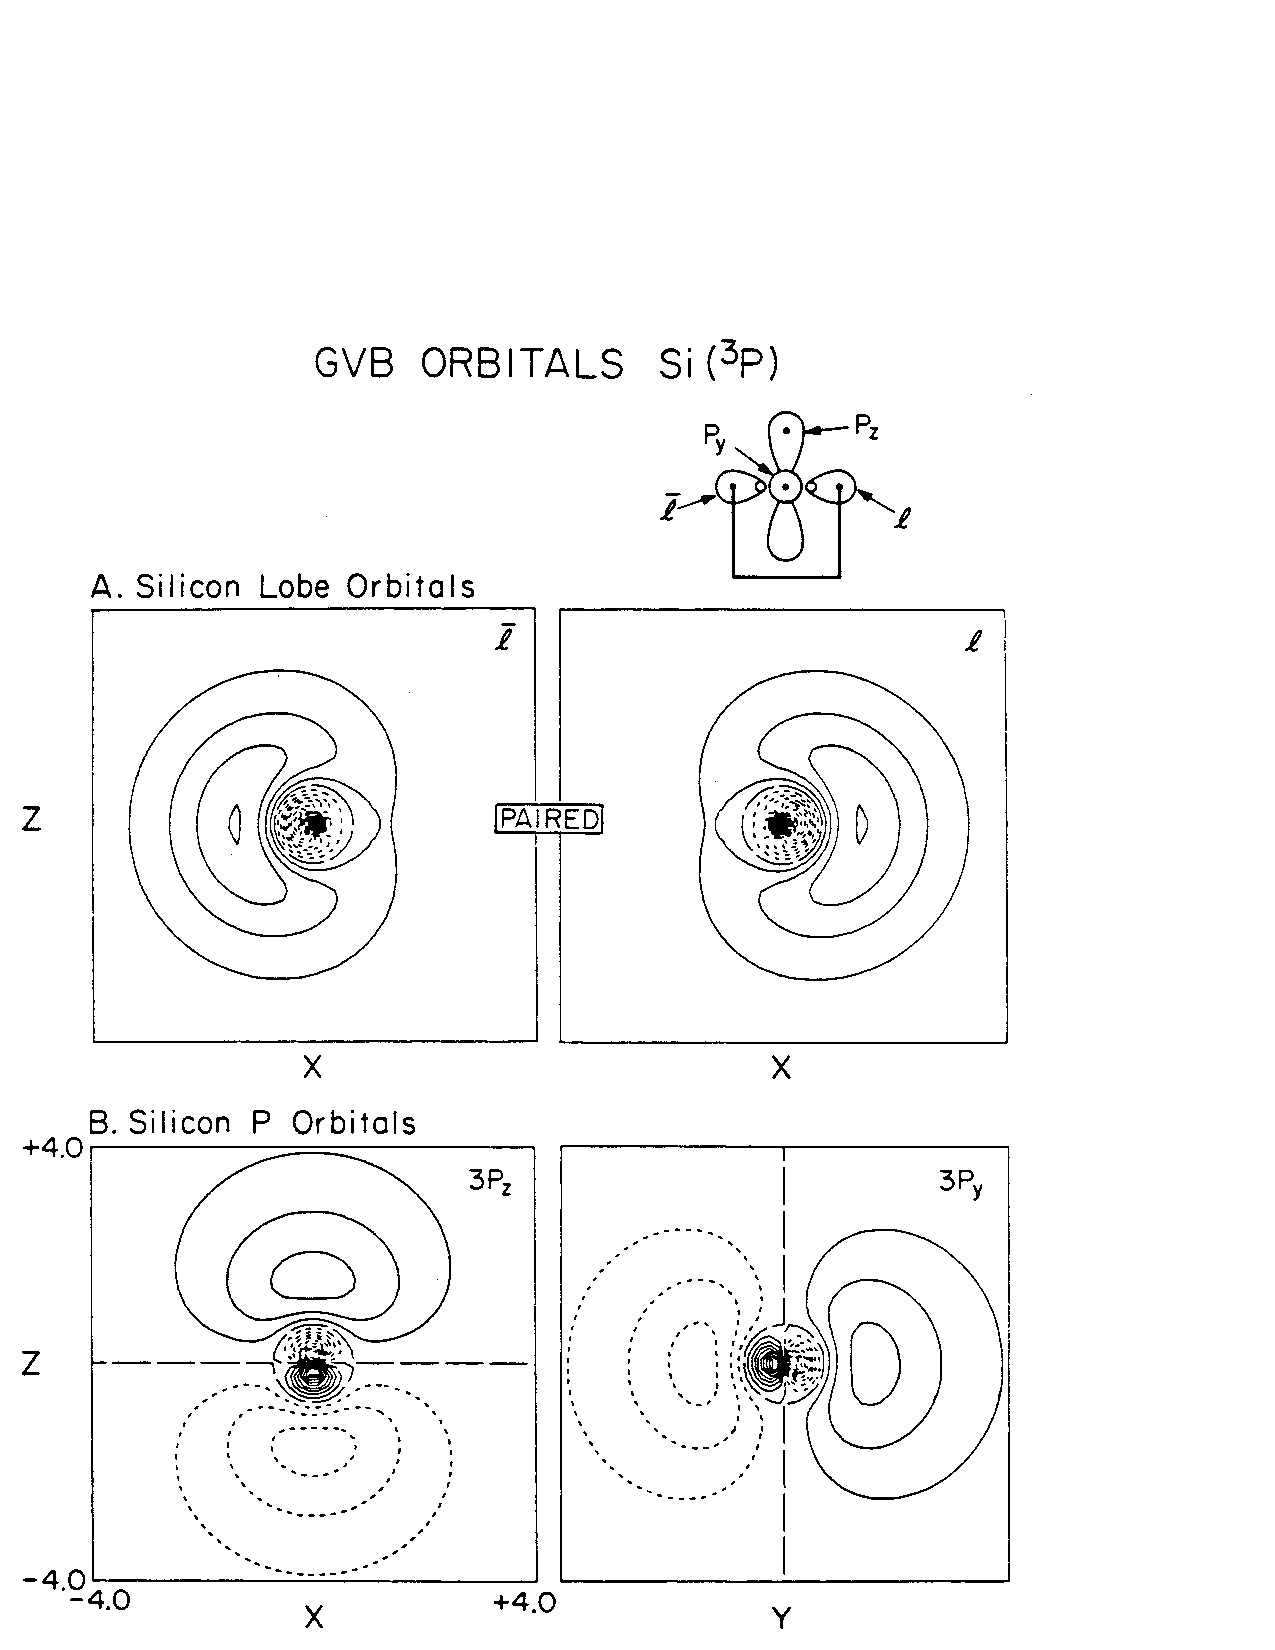
\includegraphics[scale=0.75]{fig6-01}
\caption{Si(${^3P}$)orbitals.  Long dashes indicate zero amplitude,
solid lines and short dashes indicate positive and negative amplitude,
with a space of 0.05 $a_0$ of amplitude between various contours.  The
same convention is used for all other figures.}
\label{chap6-fig1}
\end{figure}

The lobe orbitals differ radically from the HF $3s$ orbital 
in that one, $\phi_{\ell}$, is pooched, hybridized, in the positive $x$ 
direction, while the other, $\phi_{\bar{\ell}}$ is pooched in the negative $x$ 
direction.  The result is that the motion of the two $3s$ electrons is 
correlated such that they tend to stay apart while each remains close 
to the nucleus.

There are several important points to be made about the lobe orbitals 
of (\ref{chap6-eqno4}).  These orbitals can be written as
\begin{eqnarray}
\phi_{\ell} &=& {(\phi_s + \lambda \phi_{p_x} ) \over \sqrt{1 + 
\lambda^2}}\cr
\phi_{\bar{\ell}} &=& {( \phi_s - \lambda \phi_{p_x} ) \over \sqrt{1 + 
\lambda^2}}
\label{chap6-eqno5}
\end{eqnarray}
where $\phi_s$ is nearly identical to the HF $3s$ orbital,
and $\phi_{p_x}$ is nearly identical to the $\phi_{p_y}$ and
$\phi_{p_z}$ orbitals of (\ref{chap6-eqno4}).  From
(\ref{chap6-eqno5}) it can be seen that the hybridization, or
fractional $p$ character, of a lobe orbital is simply
${\lambda^2 \over (1 + \lambda^2)}$
and the overlap between the $\phi_{\ell}$ and $\phi_{\bar{\ell}}$ orbitals is
\begin{equation}
S_{\ell,{\bar{\ell}}} = s = {(1 - \lambda^2) \over (1 + \lambda^2)}
\end{equation}
or
\begin{equation}
\lambda^2 = {(1 - S) \over (1+S)} .
\end{equation}
For Si, $\lambda = 3.076$, and hence, the $\ell$ and ${\bar{\ell}}$ orbitals 
have an overlap of 0.752, and each consists of about 14.2 percent 
$p_x$ character.

Using (\ref{chap6-eqno5}), we find that
\begin{equation}
\left[ \phi_{\ell} \phi_{\bar{\ell}} + \phi_{\bar{\ell}} \phi_{\ell} 
\right] = \left[ \phi_s \phi_s - \lambda^2 \phi_{p_x} \phi_{p_x} \right] 
\left[ {2 \over (1 + \lambda^2)} \right] .
\label{chap6-eqno6a}
\end{equation}
and normalizing the right-hand side leads to
\begin{equation}
{\left[ \phi_s \phi_s - \lambda^2 \phi_{p_x} \phi_{p_x} \right] \over 
\sqrt{1+ \lambda^4}}
\label{chap6-eqno6b}
\end{equation}
Thus, the wavefunction in which one electron is always in
$\phi_{\ell}$, while the other is always in $\phi_{\bar{\ell}}$ is
exactly equivalent to the wavefunction, in which both electrons are in
$\phi_s$ part of the time, fraction = $1/(1+ \lambda^4)$, and both are
in $\phi_{p_x}$ part of the time, fraction = $\lambda^4/(1+
\lambda^4)$.  The left side of (\ref{chap6-eqno6a}) is referred to as
the \emph{generalized valence bond} orbitals.  The right side of
(\ref{chap6-eqno6a}) is the \emph{natural orbital} (NO) 
\emph{representation} of the
GVB wavefunction, and the orbitals, $\phi_s$ and
$\phi_{p_x}$, are referred to as \emph{natural orbitals}.

In order to satisfy the Pauli principle, a wavefunction of the form
(\ref{chap6-eqno6a}) must be combined with a single spin function,
$(\alpha \beta - \beta \alpha )$.  Hence, (\ref{chap6-eqno6a}) is
referred to as singlet pairing of the two lobe orbitals.  The
alternative combination
\begin{equation}
\left( \phi_{\ell} \phi_{\bar{\ell}} - \phi_{\bar{\ell}} \phi_{\ell}
\right) = \left( 
\phi_s \phi_{p_x} - \phi_{p_x} \phi_s \right) \left[ {(-2 \lambda) \over (1+ 
\lambda^2)} \right]
\label{chap6-eqno7}
\end{equation}
is referred to as \emph{triplet pairing}, since the Pauli principle
requires a triplet spin function, e.g., $\alpha \alpha$, to be
associated with (\ref{chap6-eqno7}).

Comparing the right sizes of (\ref{chap6-eqno6a}) and
(\ref{chap6-eqno7}), we see that triplet pairing of $\ell$ and
$\bar{\ell}$ forces the wavefunction to have only one electron in the
$s$ orbital, while single pairing allows a much higher $s$ occupation,
${1 \over \sqrt{1+\lambda^4}}$.
The valence $s$ orbital penetrates the core region more effectively 
than does the $p$ orbital, and is consequently less shielded from the 
nuclear charge.  Thus, the $s$ orbital is energetically more 
favorable than the $p$ orbital, and as a result, atomic states in 
which $\ell$ and $\bar{\ell}$ are singlet-paired are much lower in energy, 
approximately 100 kcal, then those in which the lobes are 
triplet-paired.

Schematically, we will represent the wavefunction in
(\ref{chap6-eqno6a}) as
\begin{equation}
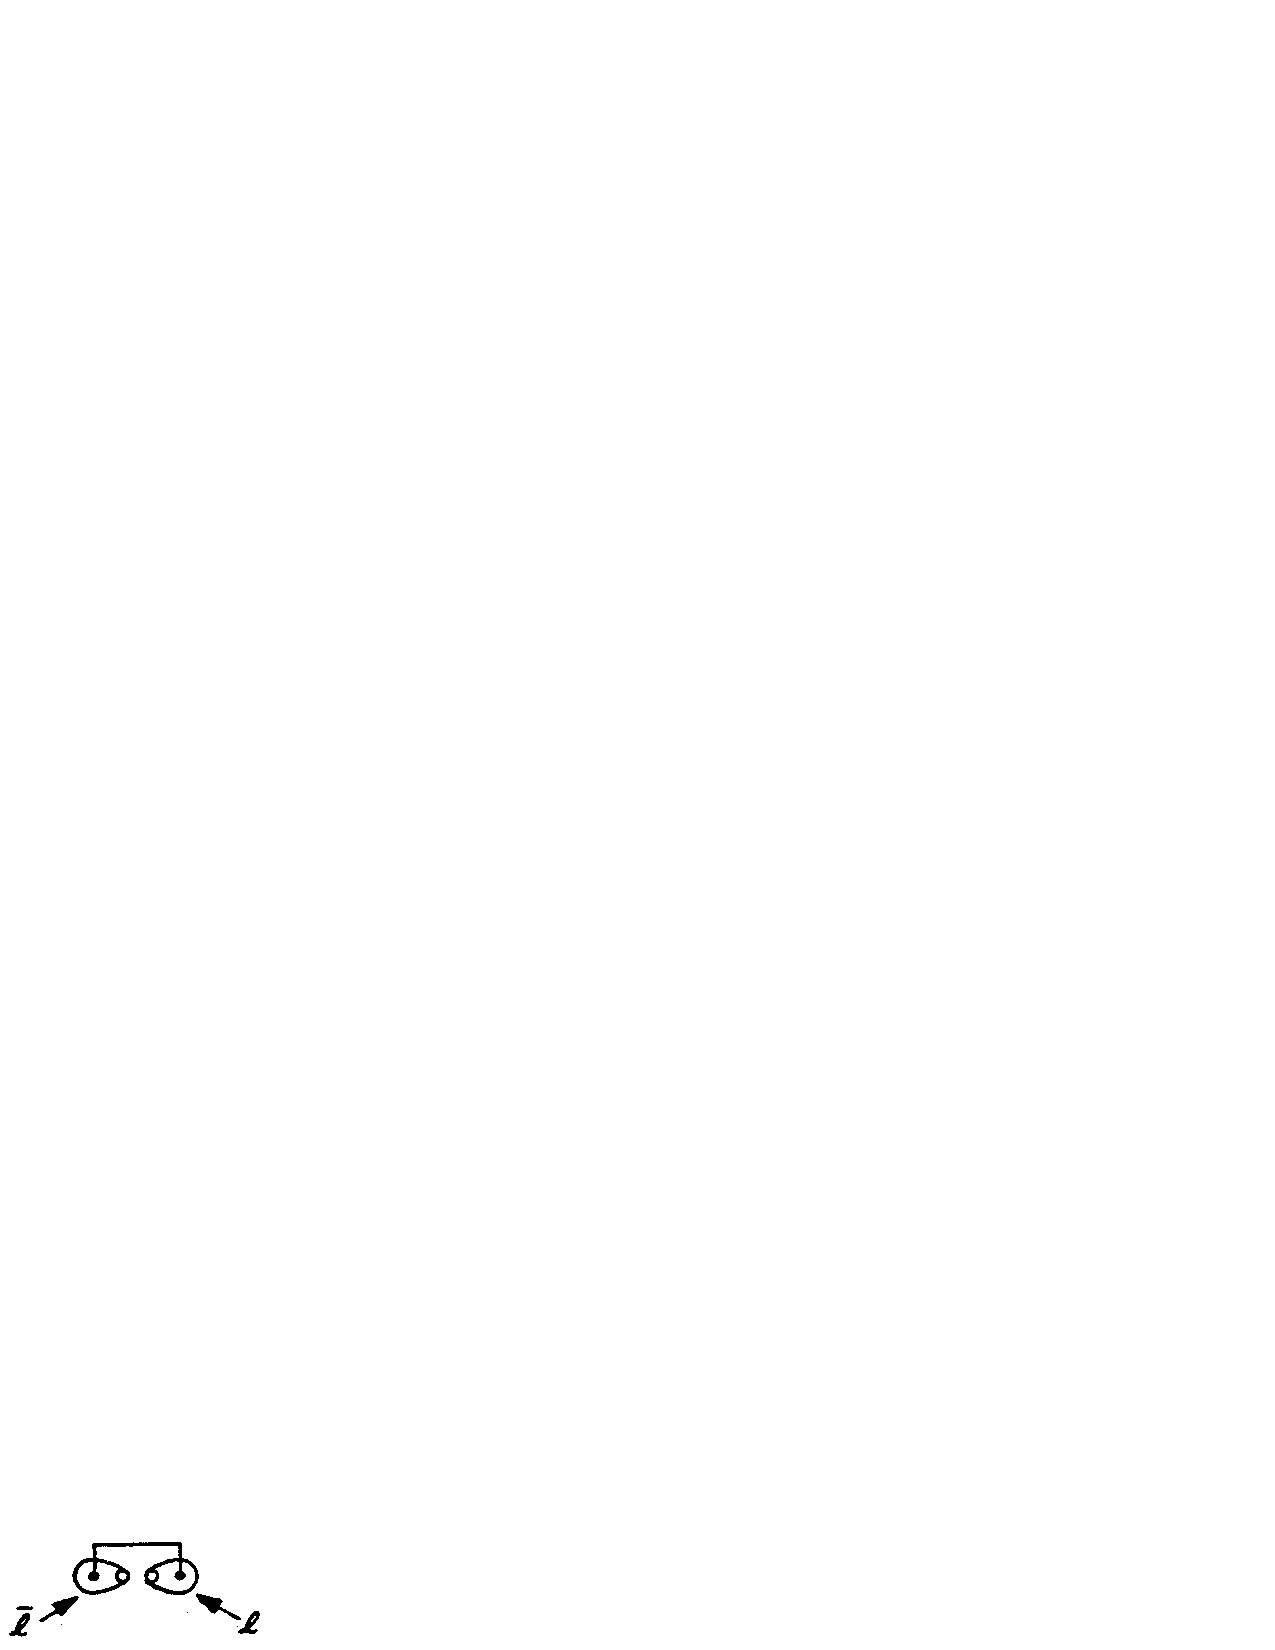
\includegraphics[scale=0.75]{fig6-01a}
\end{equation}
where 
\begin{equation}
% need an image of a lobe orbital here p 6.1-6
\end{equation}
indicates a lobe orbital, a dot indicates one electron, and the line 
connecting the dots indicates singlet pairing of the two orbitals.  
Similarly, we will represent the ground state wavefunction of 
silicon, (\ref{chap6-eqno4}) as
\begin{equation}
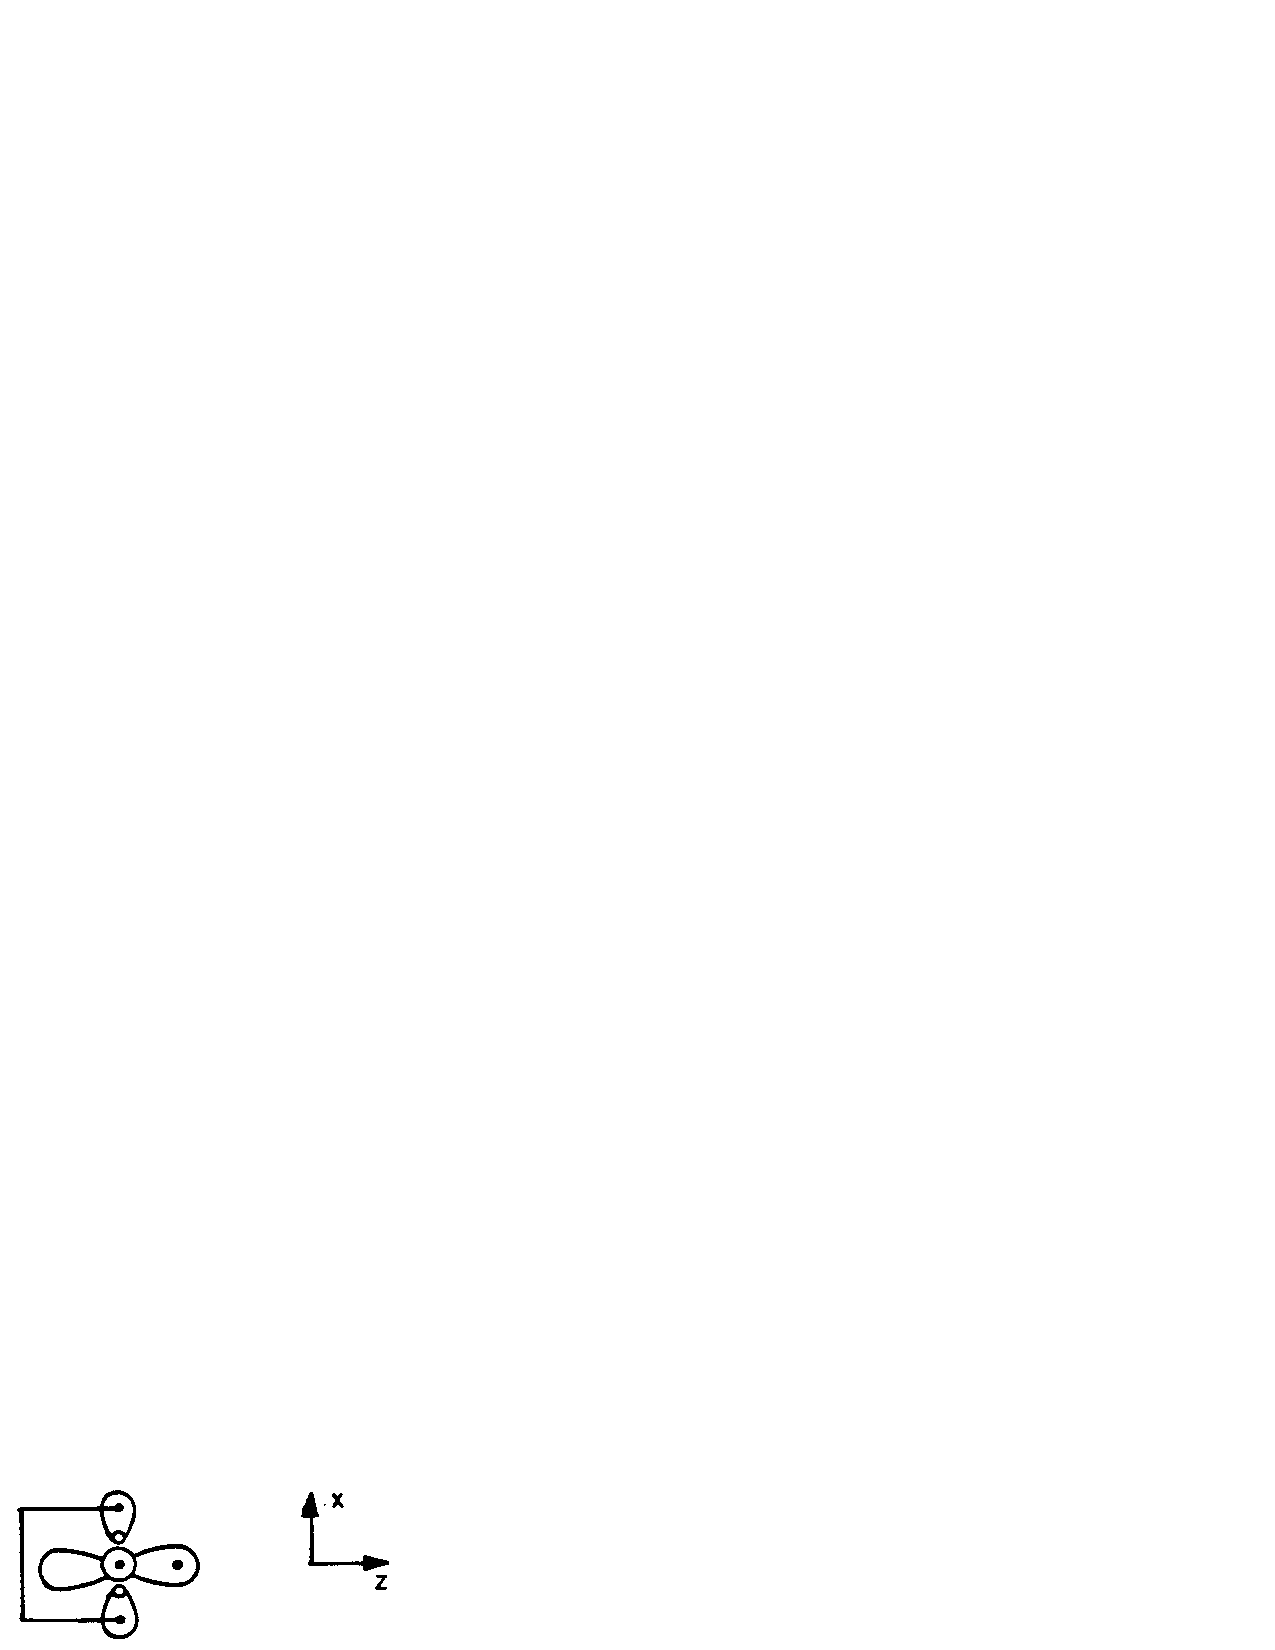
\includegraphics[scale=0.75]{fig6-01b}
\label{chap6-eqno8}
\end{equation}
where
\begin{equation}
% need an image here p_z figure 8 p 6.1-6
\end{equation}
indicates the $p_z$ orbital, and
\begin{equation}
% need an image here p_y circle p 6.1-6
\end{equation}
indicates the $p_y$ orbital, pointing out of the plane of the paper.

\subsection{Low-Lying States of SiH}

Starting with the ground state orbitals of Si, (\ref{chap6-eqno8}),
and bonding an H to one of the singly-occupied Si orbitals, we obtain
two possible configurations.  First, bonding the H to an Si $p$
orbital, leads to
\begin{equation}
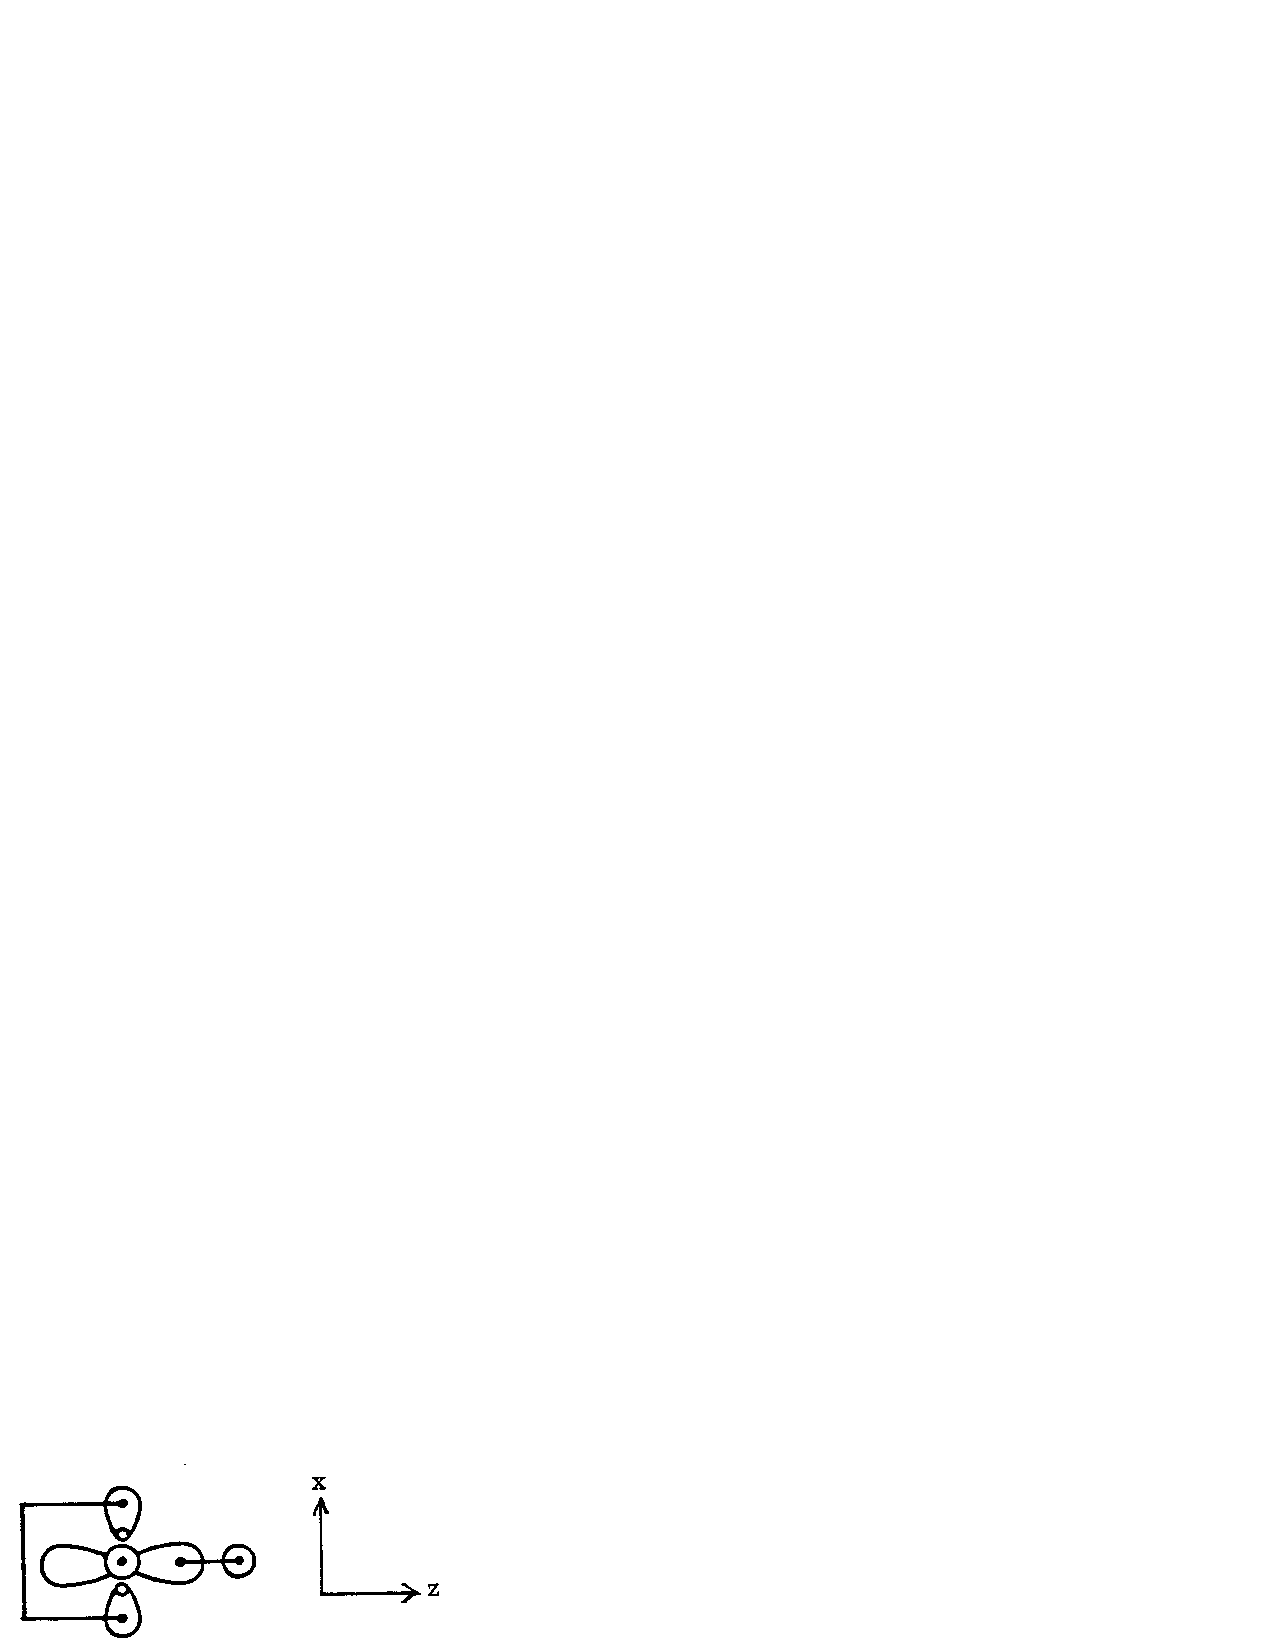
\includegraphics[scale=0.75]{fig6-01c}
\label{chap6-eqno9}
\end{equation}
which is symbolic of the wavefunction
\begin{equation}
{\cal A} \left[ \left( \phi_{\ell} \phi_{\bar{\ell}} + \phi_{\bar{\ell}} 
\phi_{\ell} 
\right) \left( \phi_{p_z} \phi_\mathrm{H} + \phi_\mathrm{H} \phi_{p_z} \right) 
\phi_{p_y} \alpha \beta \alpha \beta \alpha \right]
\end{equation}
and describes a ${^2\Pi}$ state.  Second, bonding the H to an Si 
lobe orbital, $\ell$ leads to
\begin{equation}
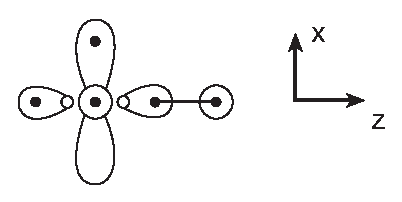
\includegraphics[scale=0.75]{fig6-01d}
\label{chap6-eqno10}
\end{equation}
which is symbolic for the wavefunction
\begin{equation}
{\cal A} \left[ \left( \phi_{\ell} \phi_\mathrm{H} + \phi_\mathrm{H}
  \phi_{\ell} \right)  \phi_{\bar{\ell}} \phi_{p_x} \phi_{p_y} \alpha
  \beta \alpha \alpha  \alpha \right]
\end{equation}
and describes a ${^4\Sigma}^-$ state.  Throughout this chapter, we
will use symmetry labels such as ${^2\Pi}$, ${^4\Sigma}^-$, ${^3B}_1$,
${^1A}_1$, etc.  The significance of the spatial symmetry, $\Pi,
\Sigma^-, B_1, A_1$, etc., will be of no importance other than
providing the label normally used to denote site.  Appendix A contains
a discussion of these symmetry names, see this appendix for linear
molecules.  The superscript is just $2S+1$, where $S$ is the spin.  In
(\ref{chap6-eqno10}), we have relabelled the axes so that the SiH bond
is along the $z$ axis.

The three unpaired orbitals of (\ref{chap6-eqno10}),
$[\phi_{\bar{\ell}} , \phi_{p_x} , \phi_{p_y} ]$ can also be coupled
to form two doublet states.  However, since these orbitals are
orthogonal, the state of highest spin, ${^4\Sigma}^-$, will be lowest
in energy.  When the orbitals are orthogonal, the argument used for
Hund's rules in atoms show that the highest spin state is lowest,
maximum negative exchange integrals.

The self-consistently calculated optimum orbitals, at $R_e$, for the
wavefunctions in (\ref{chap6-eqno9}) and (\ref{chap6-eqno10}), are
shown in Figures \ref{chap6-fig2} and \ref{chap6-fig3}, respectively.
The similarity between the molecular GVB orbitals (Figures
\ref{chap6-fig2} and \ref{chap6-fig3}) and the corresponding atomic
GVB orbitals (Figure \ref{chap6-fig1}) shows this qualitative
description of the molecular states in terms of atomic orbitals, and
shows that this is accurate.

The simple GVB model, discussed above, predicts
two-lying states for SiH, the ${^2\Pi}$ states, and the ${^4\Sigma}^-$
state.  In order to better understand the relative energies of these
two states, we must examine in more detail the bonding schemes
depicted in (\ref{chap6-eqno9}) and (\ref{chap6-eqno10}).  There is,
of course, an intrinsic difference, about 15 kcal/mole, in the bond
energy of an H to a $p$ orbital, relative to the bond energy to a lobe
orbital.  However, the major differential effects involve the
interaction of the H orbital with the orbitals not involved in the
bond.  Considering first, the ${^2\Pi}$ state, (\ref{chap6-eqno9}),
the $\phi_\mathrm{H}$ orbital positioned so as to be optimum for bonding to
$\phi_{p_z}$ will overlap the two lobe orbitals, $\phi_{\ell}$ and
$\phi_{\bar{\ell}}$.  The effect of the Pauli principle, i.e., the
determinant operator, is equivalent to forcing $\phi_\mathrm{H}$ to be
orthogonal to $\phi_{\ell}$ and $\phi_{\bar{\ell}}$.  This raises the
total energy, and hence, decreases the bond energy.  All orbitals
readjust to minimize this effect and, as seen in Figure
\ref{chap6-fig2}, the major result is that the lobe orbitals,
$\phi_{\ell}$ and $\phi_{\bar{\ell}}$, rotate away from the bond pair.
Thus, in the molecule, the angular of the lobe orbitals with respect
to the $z$ axis is$^8$ 128$^{\circ}$ compared with an angle of
90$^{\circ}$ for the free atom.

\begin{figure}
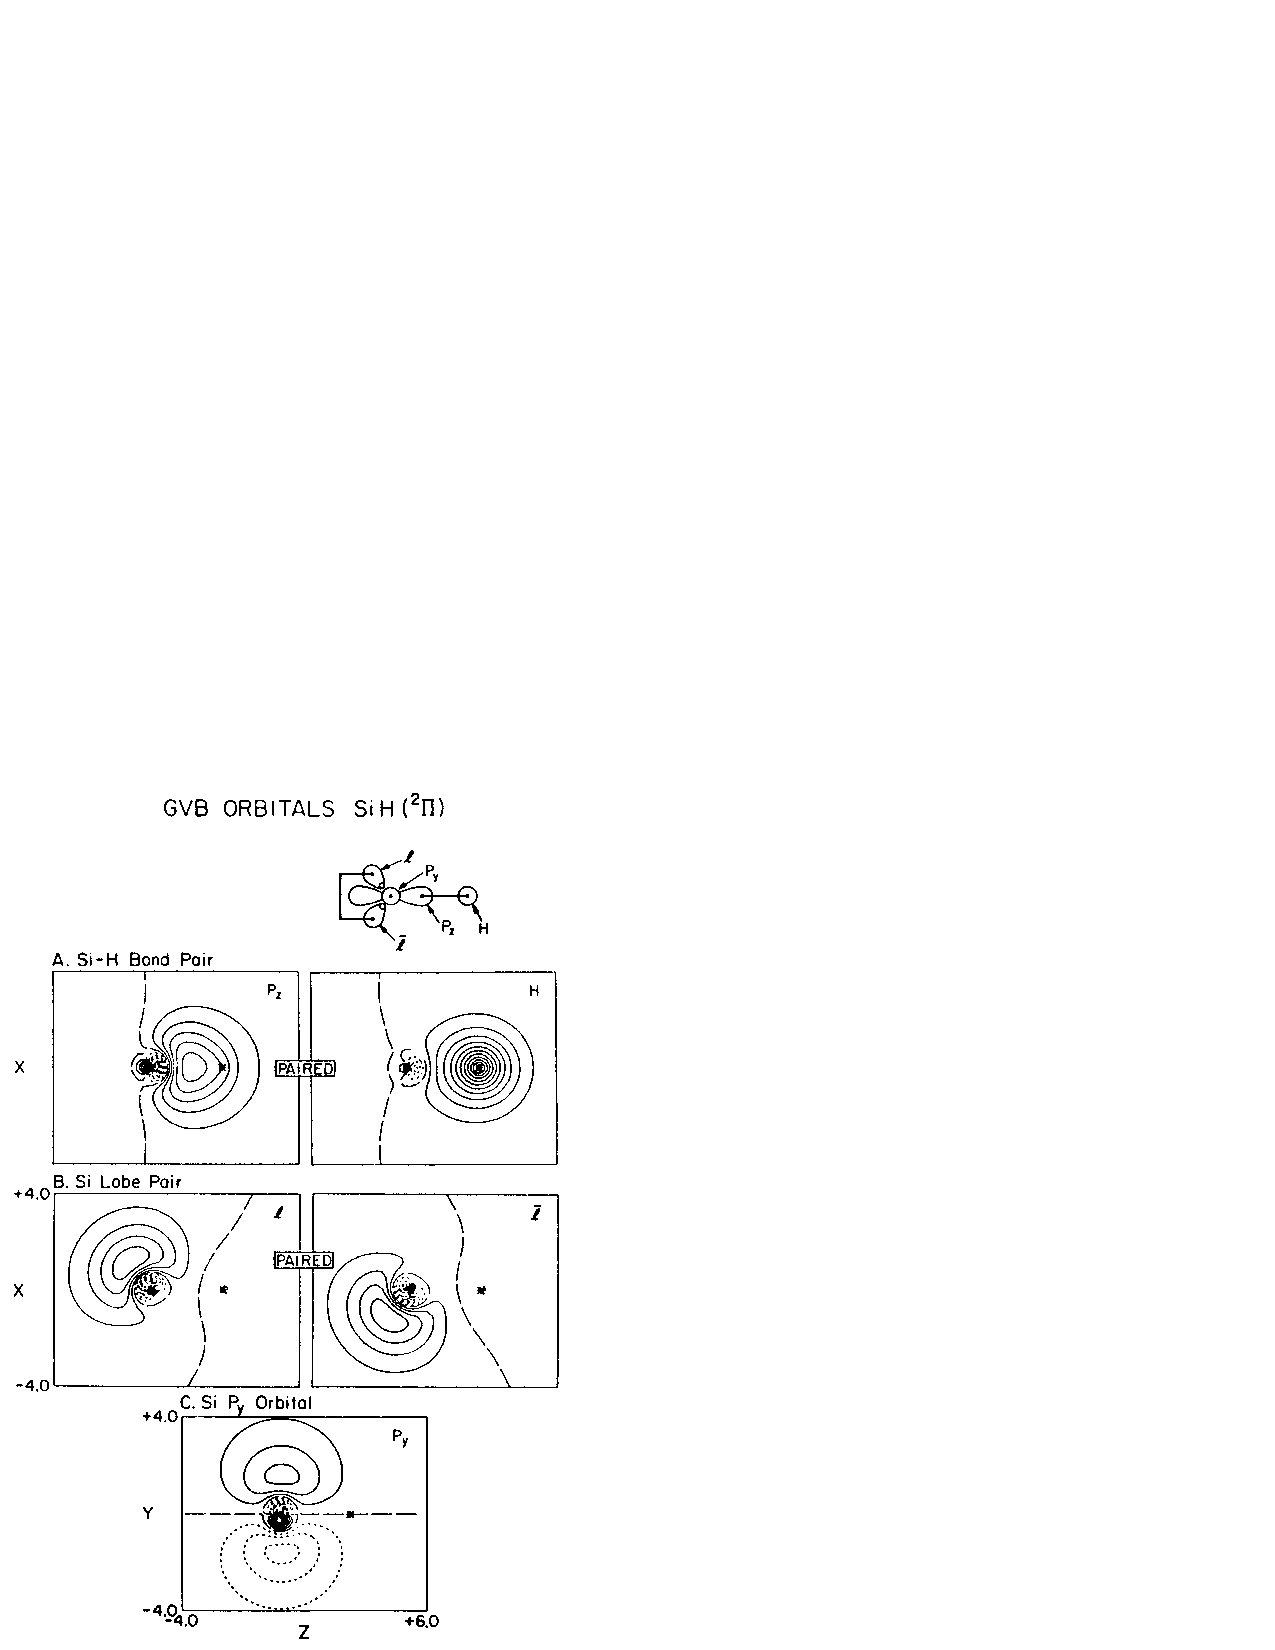
\includegraphics{fig6-02}
\caption{SiH $(^2\Pi)$ orbitals.}
\label{chap6-fig2}
\end{figure}

\begin{figure}
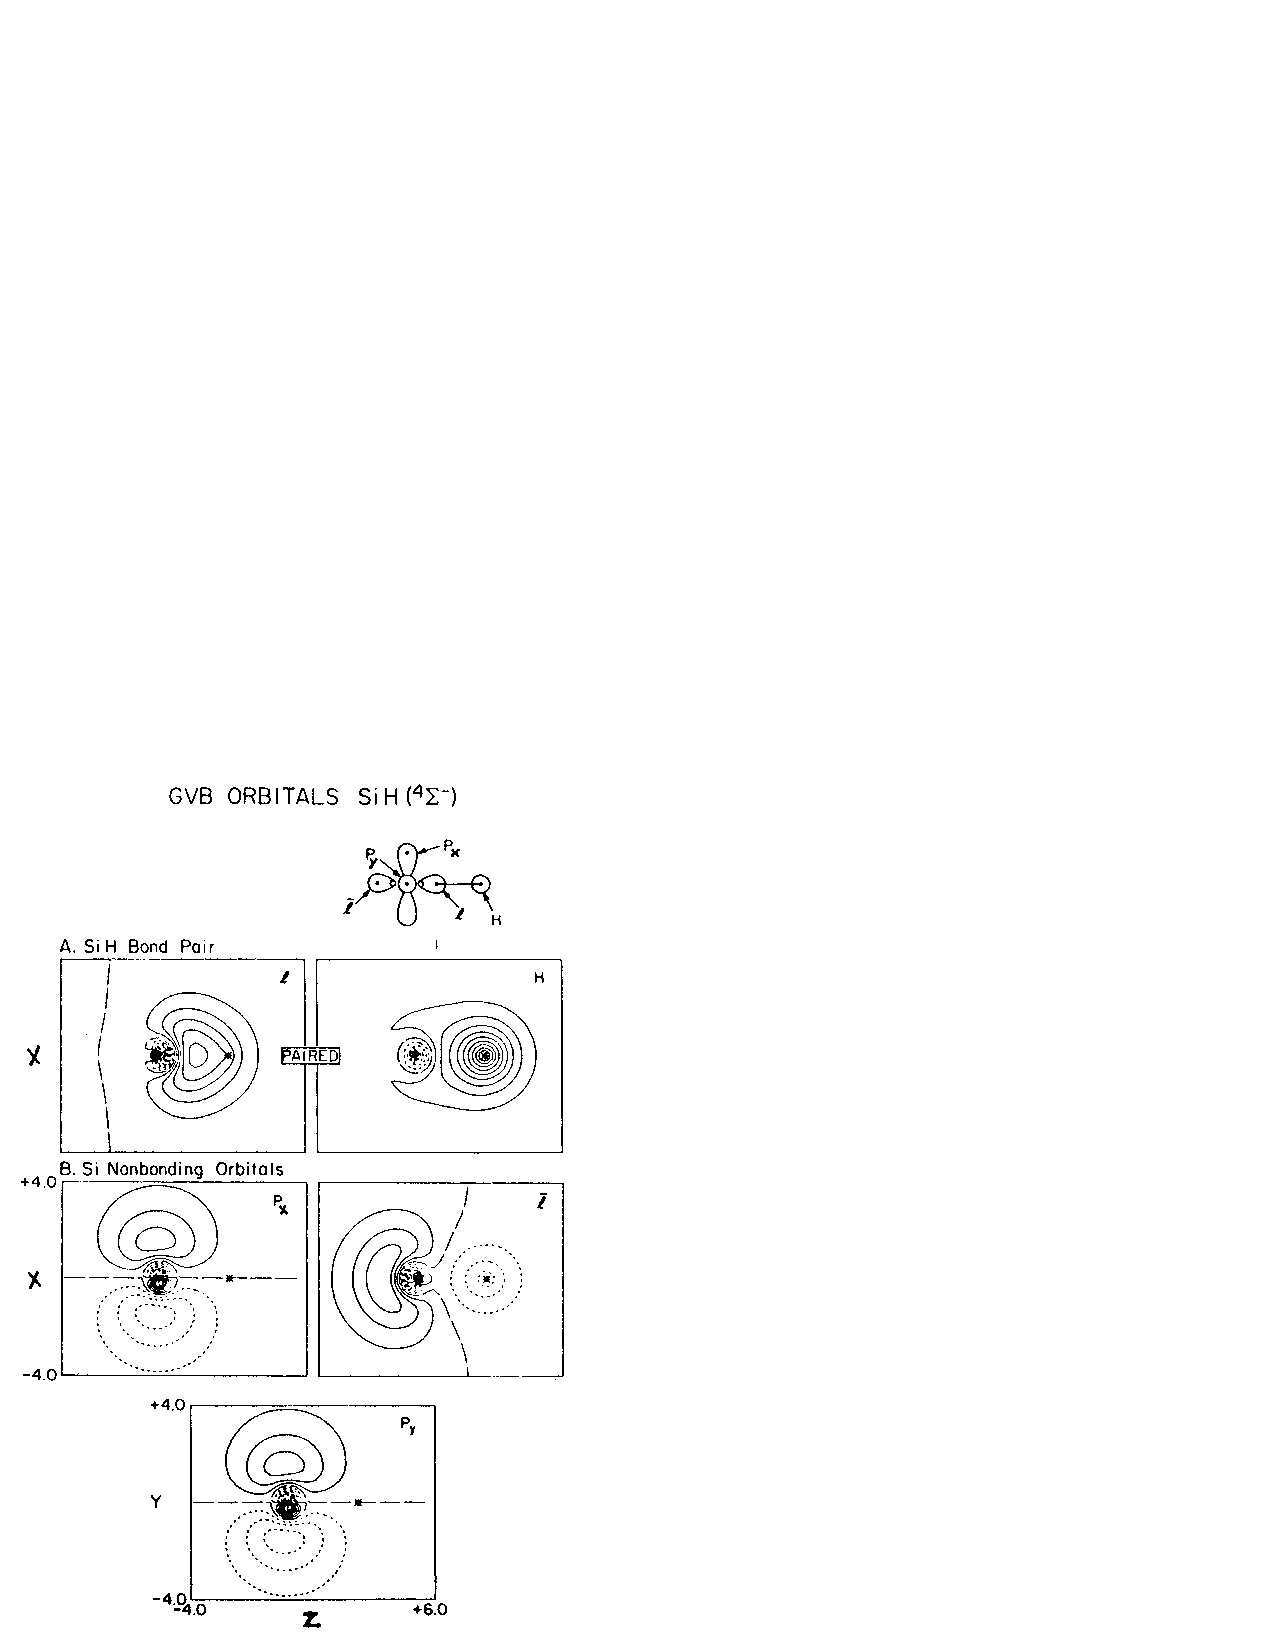
\includegraphics{fig6-03}
\caption{SiH $(^4\Sigma^-)$ orbitals.}
\label{chap6-fig3}
\end{figure}

Consider now the bonding scheme in the ${^4\Sigma}^-$ state of SiH,
(\ref{chap6-eqno10}).  In the atom $\phi_{\ell}$ and
$\phi_{\bar{\ell}}$ are singlet-paired, and the optimum orbitals have
an overlap of 0.752, whereas in the molecular, the $\phi_{\ell}$
orbital is singlet-paired with $\phi_\mathrm{H}$.  Again, because of the Pauli
principle, the $\phi_{\bar{\ell}}$ orbital of the molecule must become
orthogonal to the $(\phi_{\ell} , \phi_\mathrm{H})$ bond orbitals, leading to
an increase in the total energy of this state.  This repulsive effect,
resulting from the unpairing of the $(\phi_{\ell} ,
\phi_{\bar{\ell}})$ orbitals, leads to a new bond energy much smaller
than the intrinsic bond energy for the lobe orbital.  In the optimized
wavefunction, the bond and nonbonding orbitals have readjusted to
minimize the repulsive interaction, leading to the GVB
orbitals shown in Figure \ref{chap6-fig3}.

In conclusion, the atomic origins of the self-consistent GVB
orbitals of both the ${^2\Pi}$ and ${^4\Sigma}^-$ 
states, is clearly recognizable.  In particular, the bond pair of 
the ${^4\Sigma}^-$ state involves an Si-centered orbital that is more 
lobe-like than the Si-centered bond orbital of the ${^2\Pi}$ state.  
Including all effects, the bond of an H to a $p$ orbital of Si, 
forming the ${^2\Pi}$ state, is 70 kcal, while the bonding to a 
lobe orbital is 35 kcal.  However, it should be emphasized that the 
weakness of the lobe bond, relative to the $p$ bond, is due almost 
entirely to the energy required to uncouple the atomic $(\ell , 
{\bar{\ell}})$ pair, as described.

\subsection{Low-lying States of SiH$_2$}

Consider now, the state of SiH$_2$ that result from bonding a hydrogen 
to the ground state of SiH,
\begin{equation}
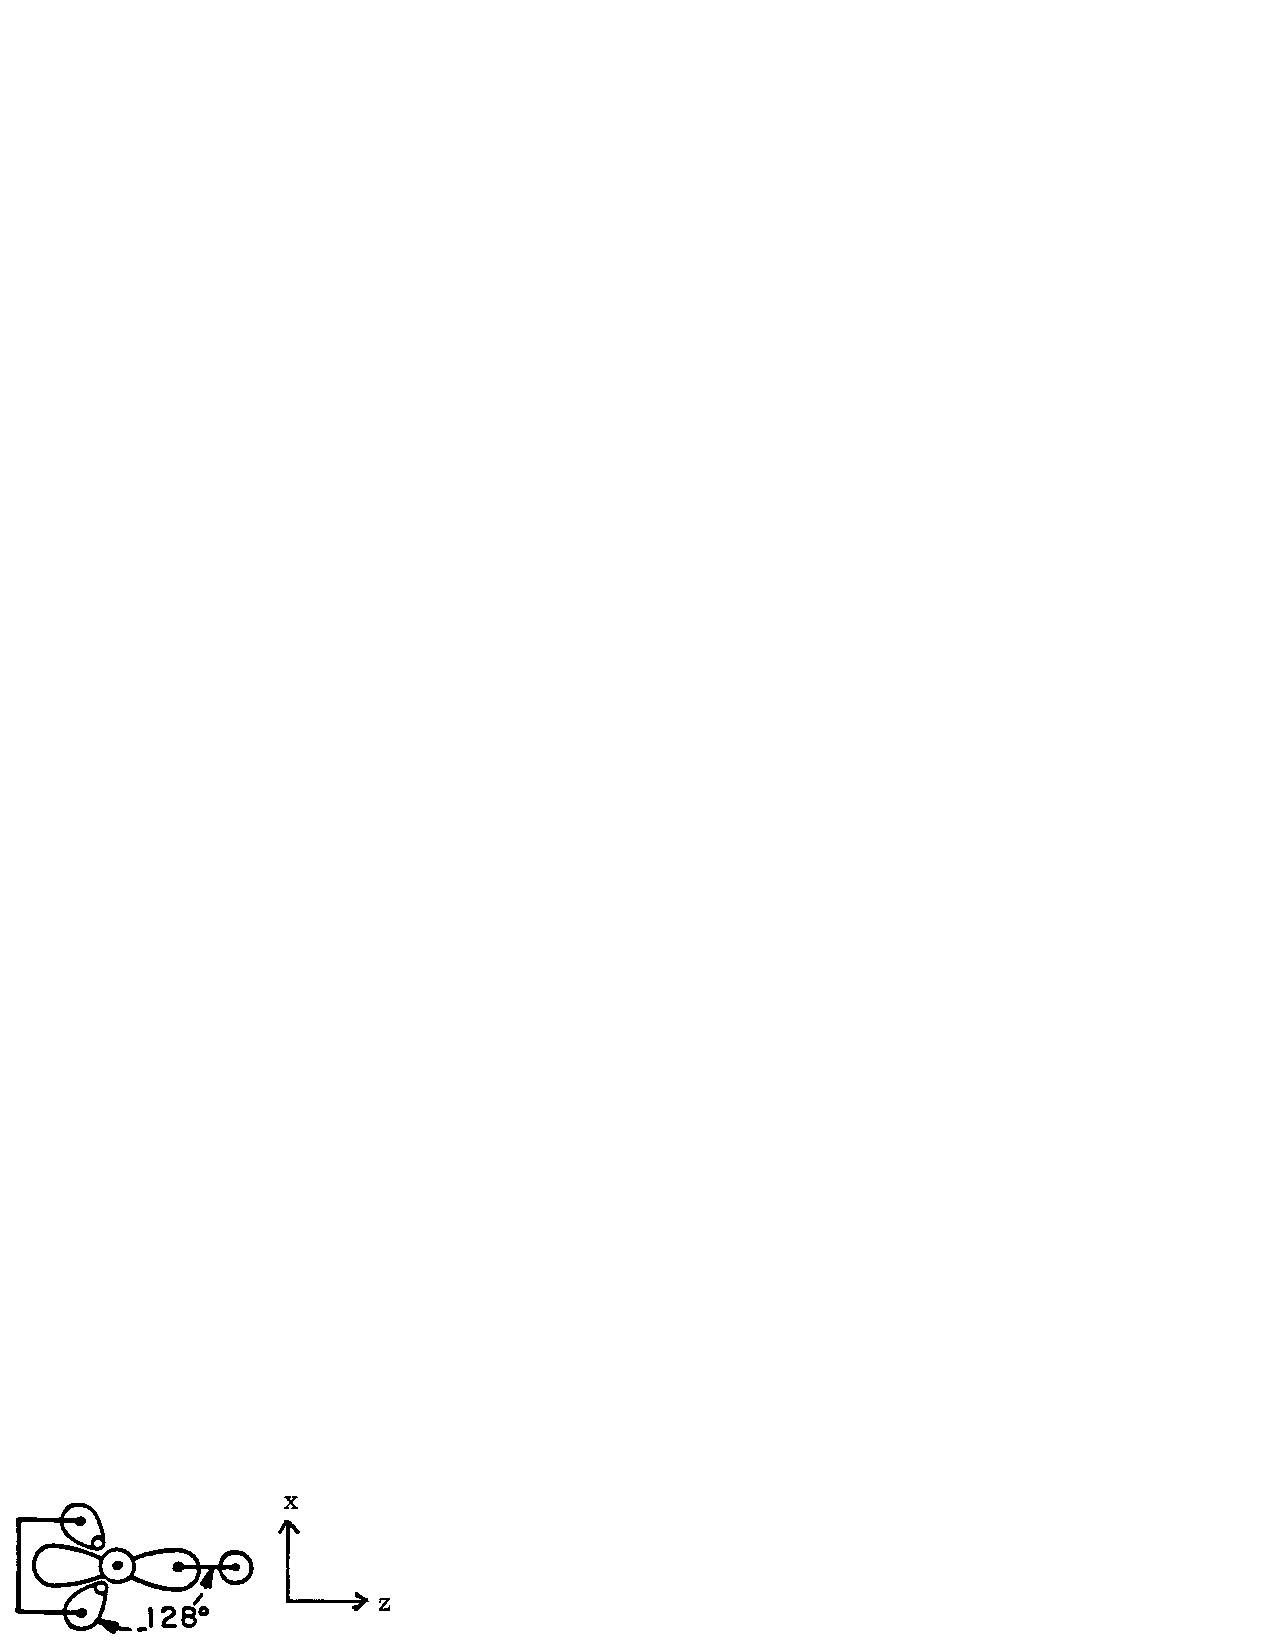
\includegraphics[scale=0.75]{fig6-03a}
\label{chap6-eqno11}
\end{equation}
Just as for SiH, we can form a strong bond to either the unpaired Si 
$p$ orbital, or to one of the paired lobe orbitals.  Bonding the H to 
the $p$ orbital, $(p_y)$, leads to the ${^1A}_1$ state of SiH$_2$,
\begin{equation}
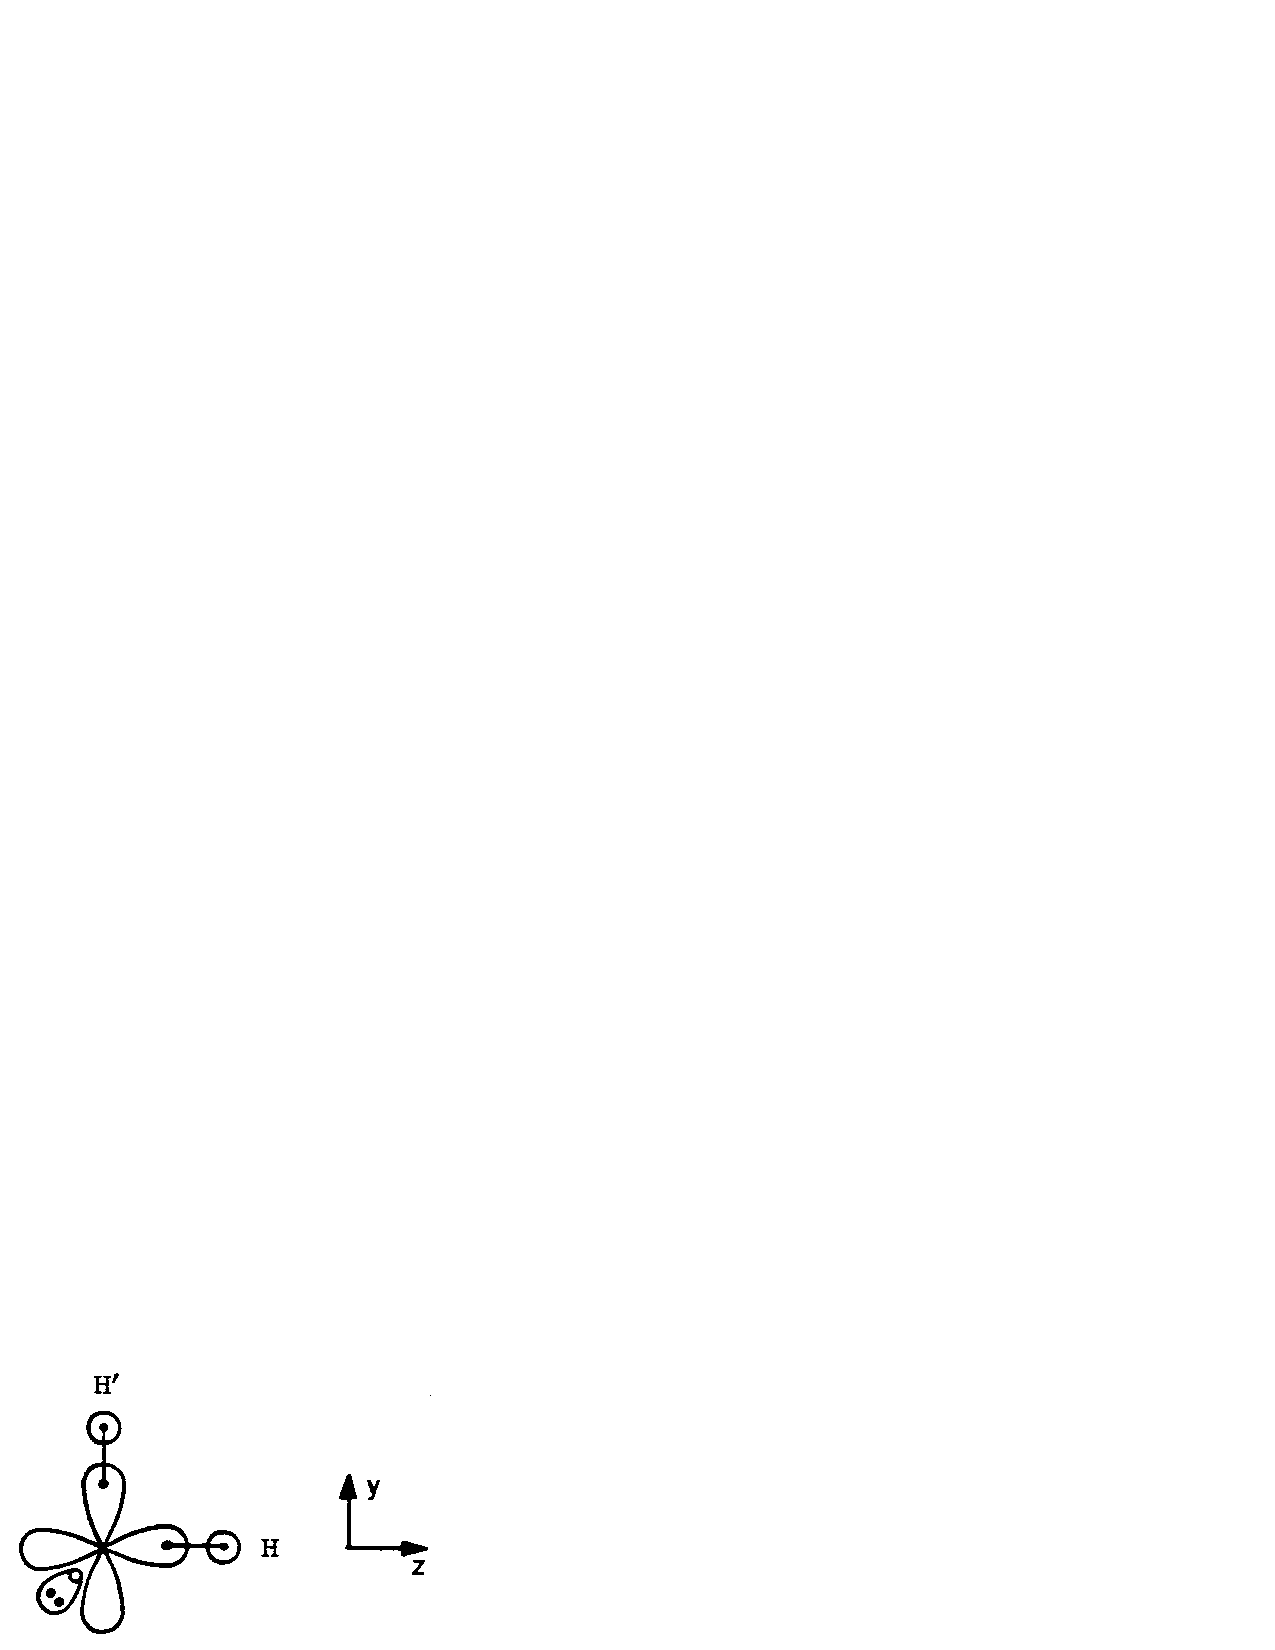
\includegraphics[scale=0.75]{fig6-03b}
\label{chap6-eqno12}
\end{equation}
which is symbolic for the wavefunction
\begin{equation}
{\cal A} \left[ \left( \phi_{\ell} \phi_{\bar{\ell}} +
\phi_{\bar{\ell}} \phi_{\ell} \right) \left( \phi_{p_z}
\phi_\mathrm{H} + \phi_\mathrm{H} \phi_{p_z} \right) \left( \phi_{p_y}
\phi_{\mathrm{H}^{\prime}} + \phi_{\mathrm{H}^{\prime}} \phi_{p_y}
\right) \alpha \beta \alpha \beta \alpha \beta \right] ,
\end{equation}
where
\begin{equation}
% missing doubly-occupied lobe orbital here, p 6.1-10
\end{equation}
represents the two overlapping lobe orbitals, one pointing above the
plane of the page and the other below.  Since the Si $p$ orbitals are
at 90$^{\circ}$ with respect to each other, one would expect the bond
angle of this state to be about 90$^{\circ}$.  Because of the Pauli
principle-induced pair-pair repulsions between the two SiH bonds, the
actual bond angle is slightly larger, 92.1.$^{9,10}$ Similarly, due to
the interaction between the lobe pair and the two SiH bond pairs, the
lobe orbitals will be in the plane bisecting the H-Si-H angle, and the
angle between the two lobes will be less than the 104$^{\circ}$ of
${^2\Pi}$ SiH, $104 = 360 - 2 \times 128^{\circ}$.  The actual optimum
angle is 90$^{\circ}$,$^{10}$ as indicated in (\ref{chap6-eqno12}).
The optimum orbitals are shown in Figure \ref{chap6-fig5}.
\begin{equation}
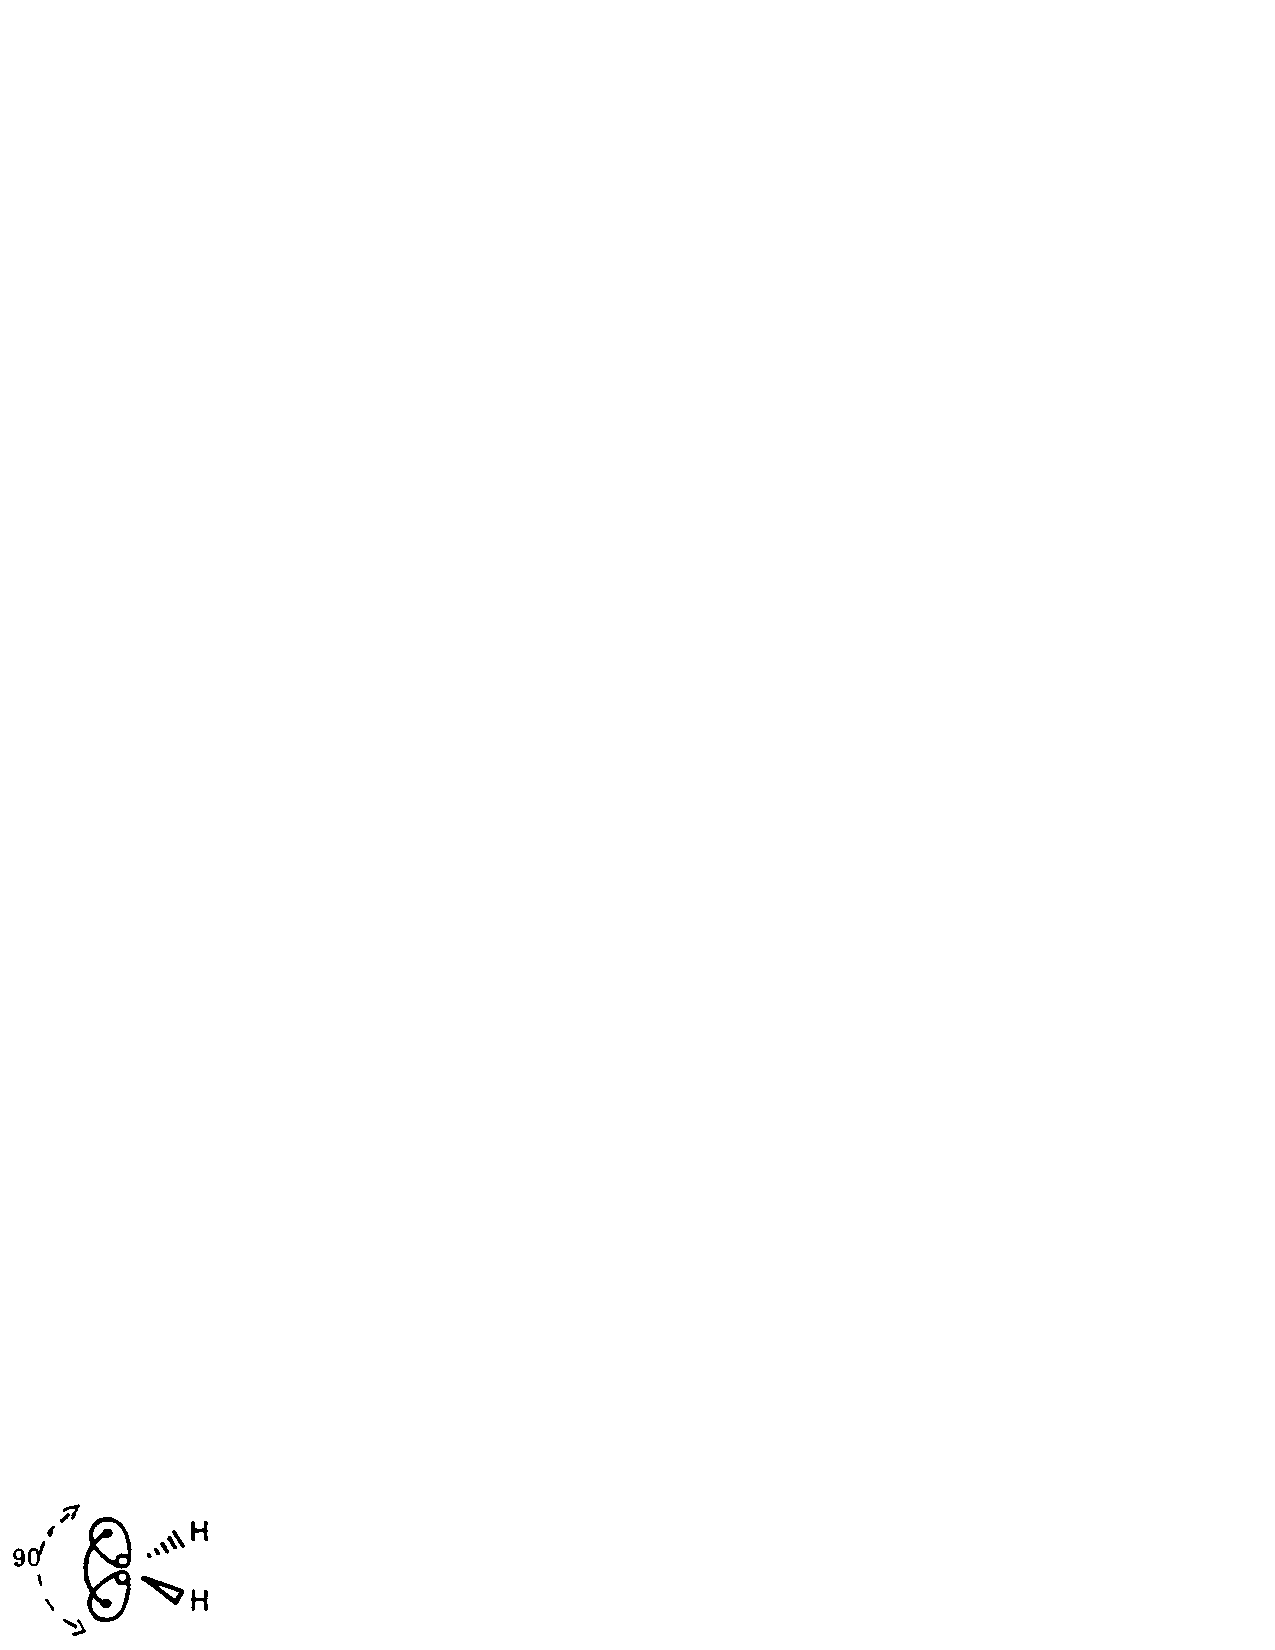
\includegraphics[scale=0.75]{fig6-03c}
\label{chap6-eqno12-a}
\end{equation}

Bonding the H to a lobe orbital of (\ref{chap6-eqno11}), leads to
\begin{equation}
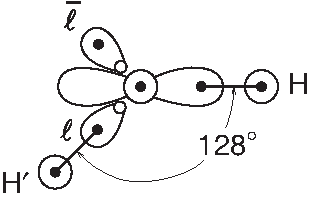
\includegraphics[scale=0.75]{fig6-03d}
\label{chap6-eqno13}
\end{equation}
In the optimum wavefunction, the orbitals comprising the two bond 
pairs will be equivalent, each having the character of roughly the 
average of a lobe bond and a $p$ bond, as depicted
\begin{equation}
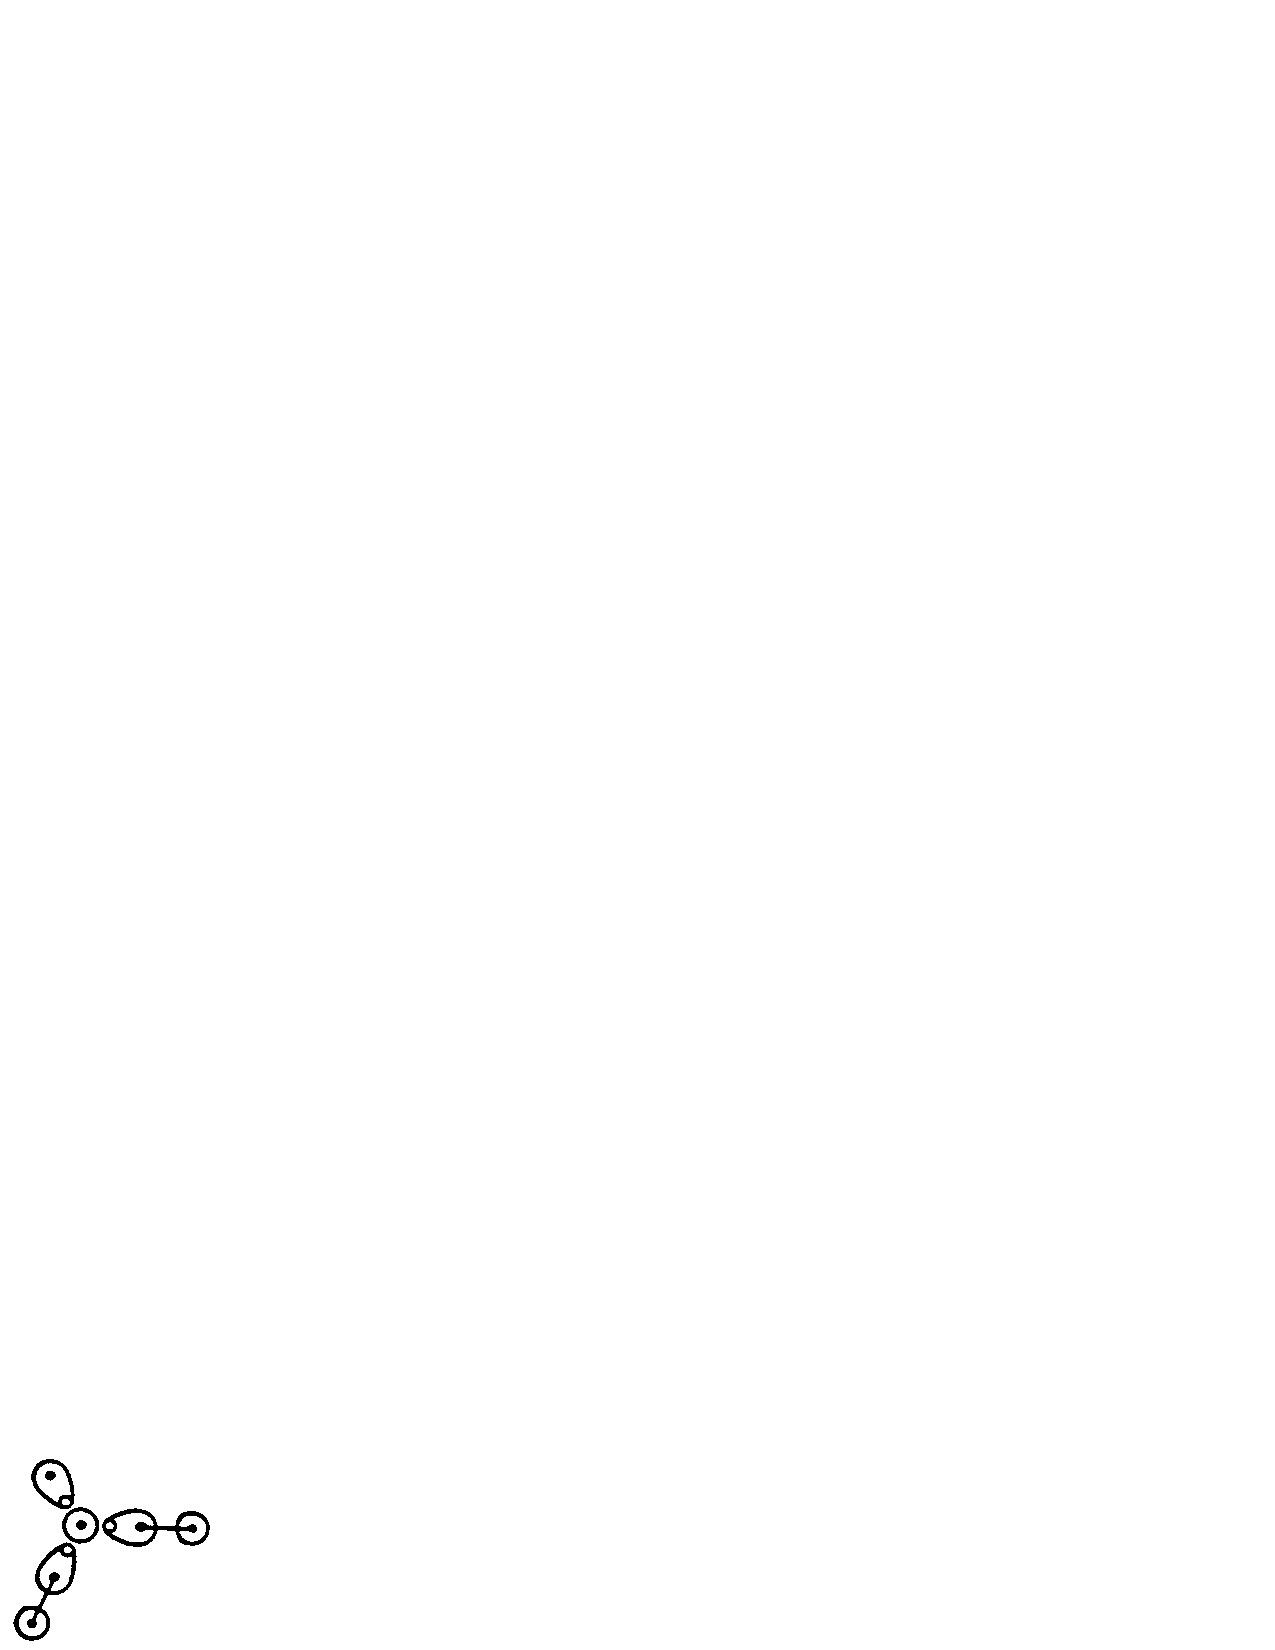
\includegraphics[scale=0.75]{fig6-04a}
\label{chap6-eqno14}
\end{equation}
From (\ref{chap6-eqno11}), the HSiH bond angle in (\ref{chap6-eqno13})
would be expected to be 128$^{\circ}$.  However, there are several
important interactions to be considered.  As the second H approaches
the lobe orbital $\ell$, the $\phi_\mathrm{H}$ orbital will overlap not only
$\ell$ but also $\bar{\ell}$, and the other SiH bond pair.  Because
the wavefunction must satisfy the Pauli principle, these overlaps give
rise to repulsive interactions.  Of the two, the H$-{\bar{\ell}}$
interaction will be more important, the $\bar{\ell}-\ell$ angles is
104$^{\circ}$, while $\ell$ is 120$^{\circ}$ from the first bond.
Thus, these repulsions will reduce the bond angle for the expected
128$^{\circ}$.  In fact, the actual bond angle is
117$^{\circ}$,$^{9,10}$ putting the lobe orbital $\bar{\ell}$ at
121-1/2$^{\circ}$ away from each bond.  The optimum orbitals are shown
in Figure \ref{chap6-fig5}.

\begin{figure}
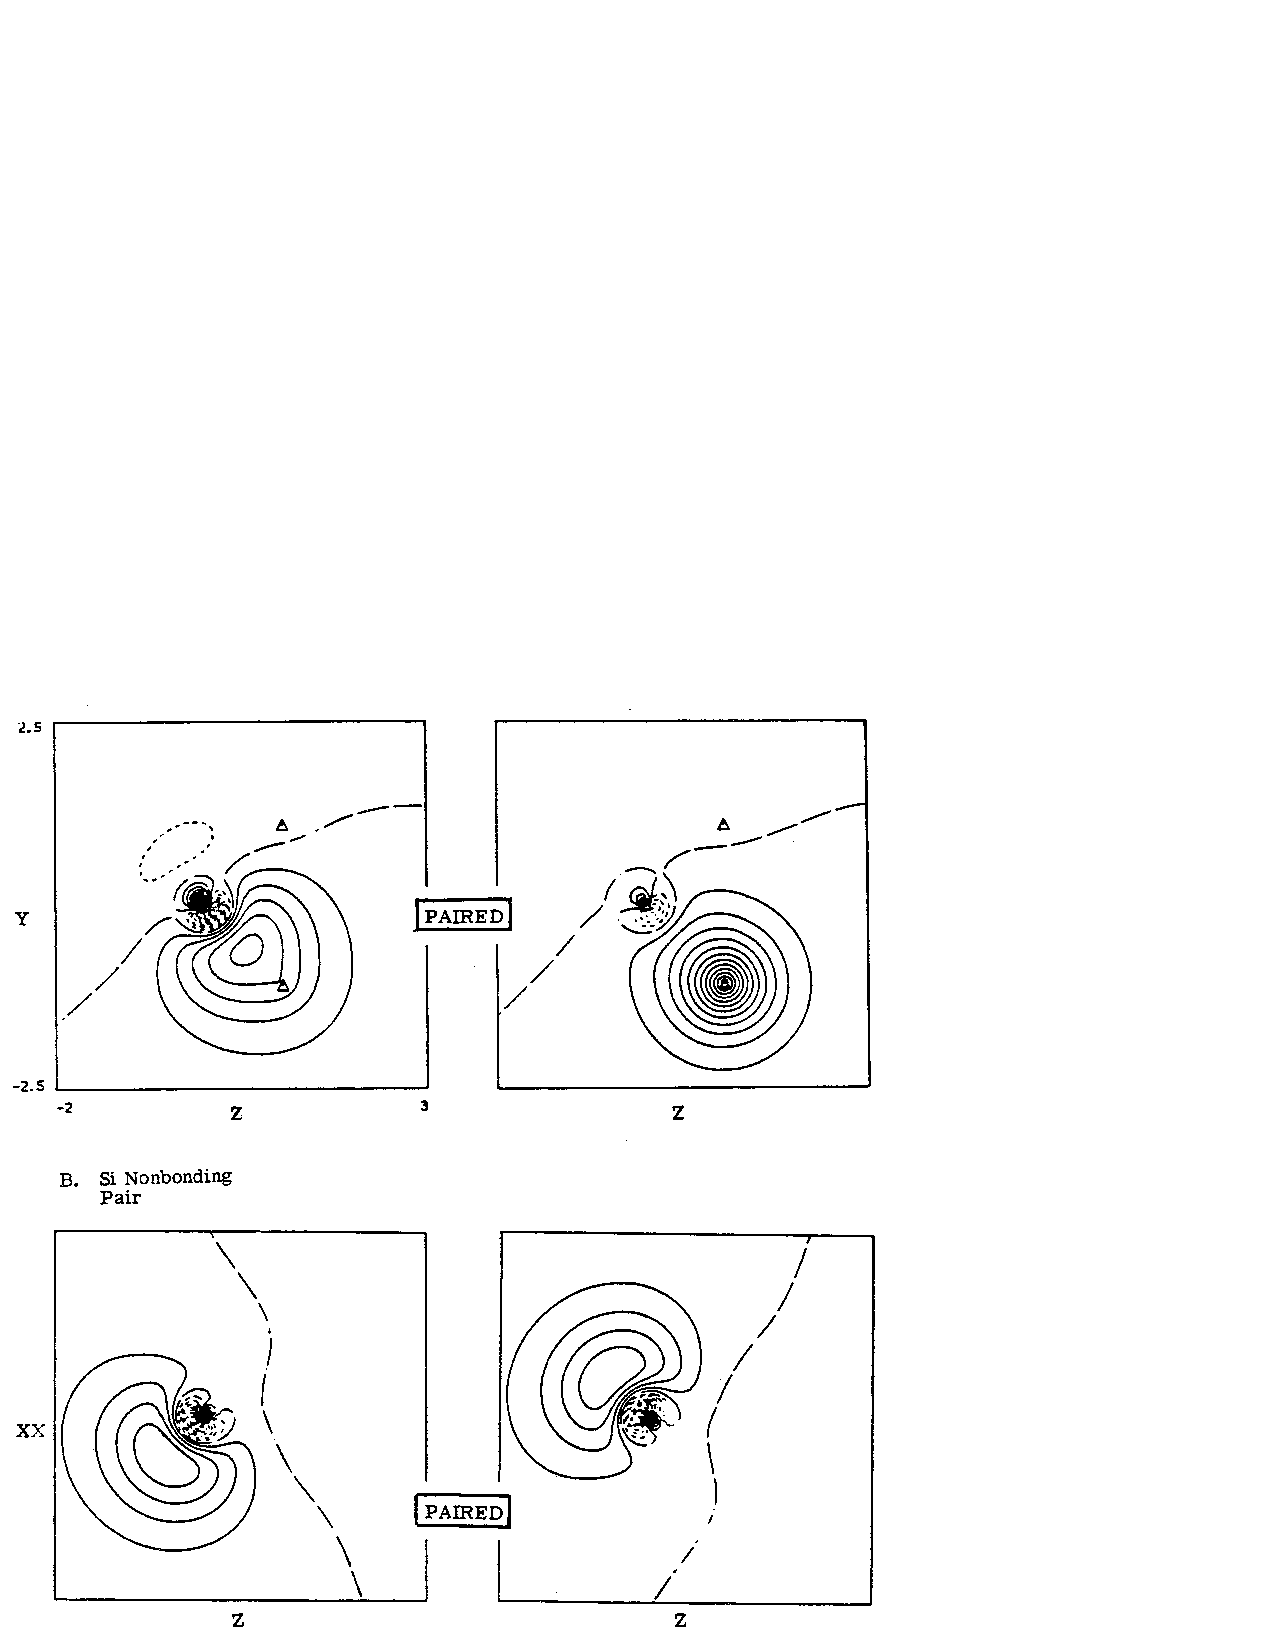
\includegraphics[scale=0.75]{fig6-04}
\caption{SiH bonding (top) and nonbonding (bottom) pairs.}
\label{chap6-fig4}
\end{figure}

\begin{figure}
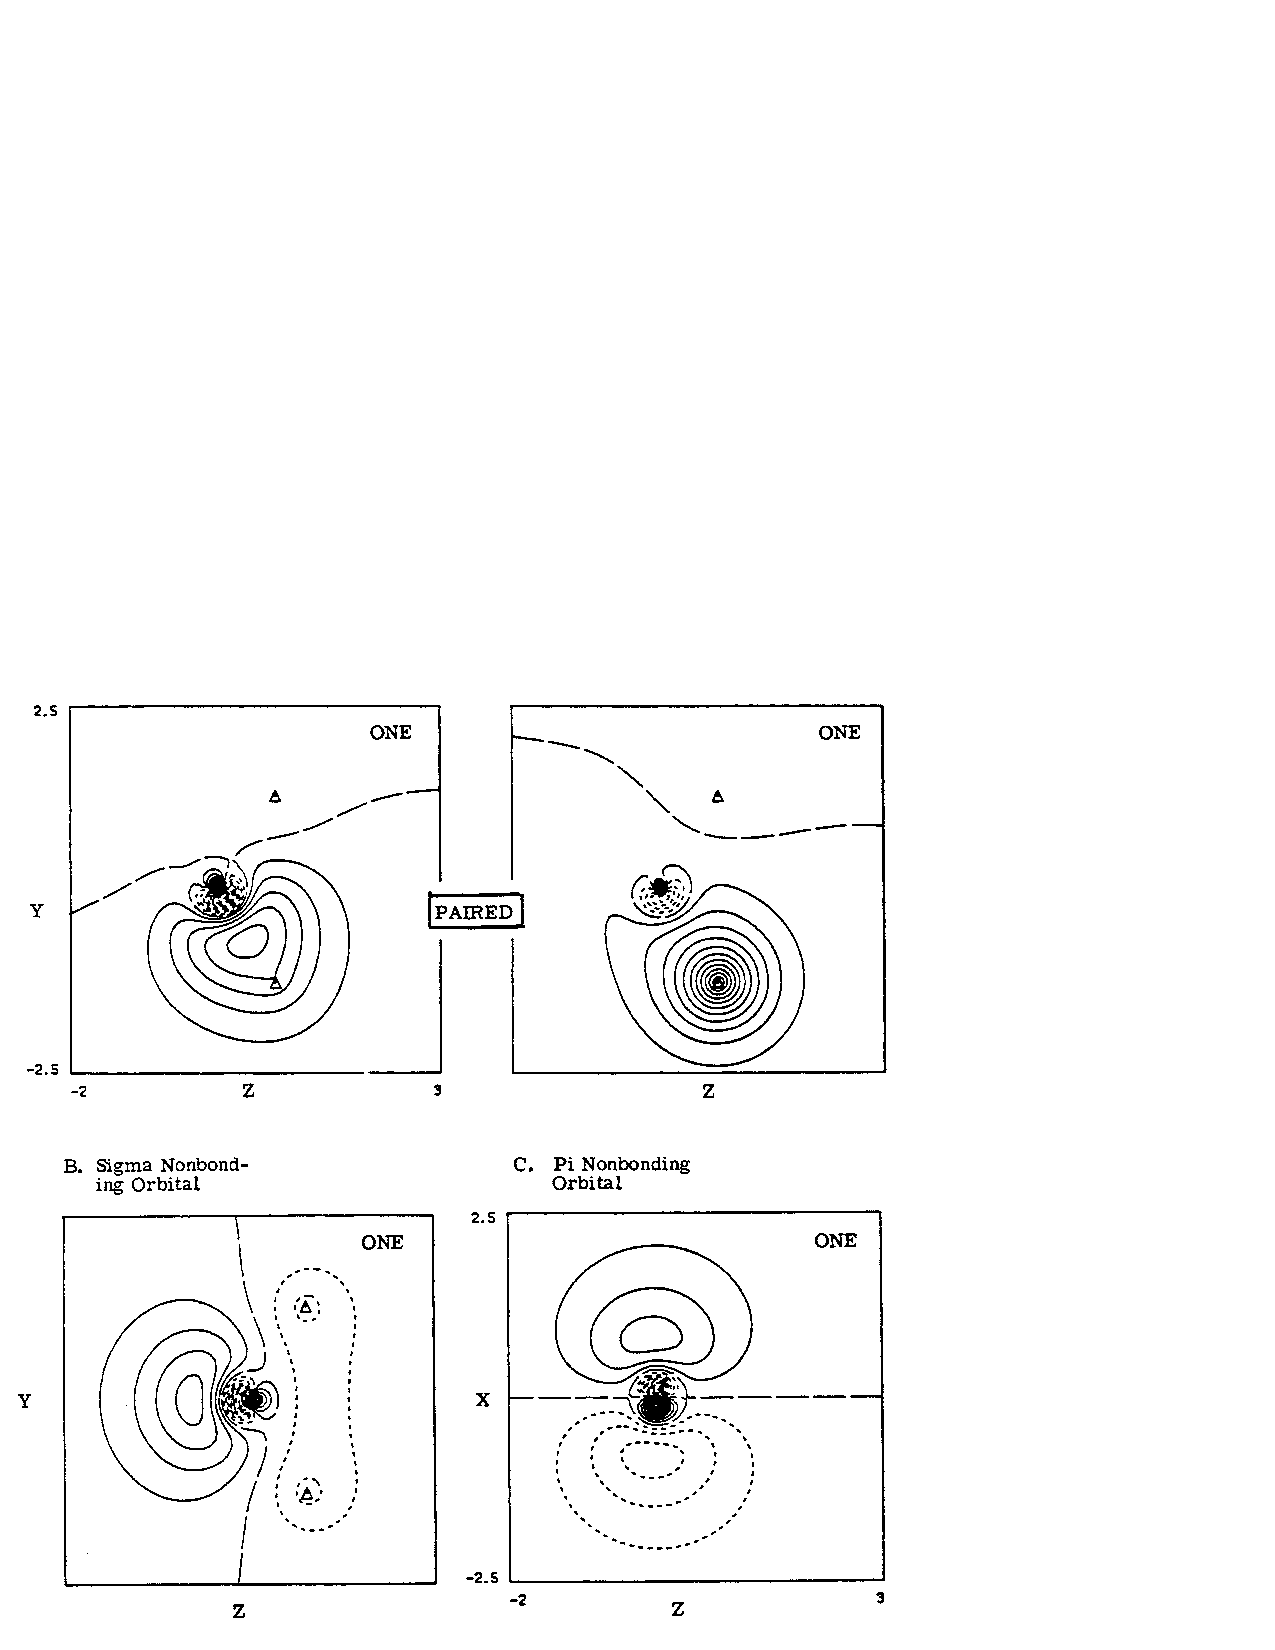
\includegraphics[scale=0.75]{fig6-05}
\caption{SiH$_2$ bonding (top) and nonbonding (bottom) pairs.}
\label{chap6-fig5}
\end{figure}

For SiH we found that bonding the hydrogen to a $p$ orbital of Si,
leads to a stronger bond than bonding to a lobe orbital, due to the
energy required to uncouple the atomic lobe pair.  Similarly, for
SiH$_2$, the strongest bond is obtained by bonding the H to the
unpaired $p$ orbital of SiH leading to the ${^1A}_1$ ground state for
SiH$_2$.  The ${^3B}_1$ state, (\ref{chap6-eqno14}), is 17.2 kcal
higher.$^{10}$

\subsection{Low-lying States of SiH$_3$ and SiH$_4$}

Starting with the ground state ${^1A}_1$ of SiH$_2$,
(\ref{chap6-eqno12}), we see that bonding a third H to SiH$_2$ should
lead to a pyramidal molecule as
\begin{equation}
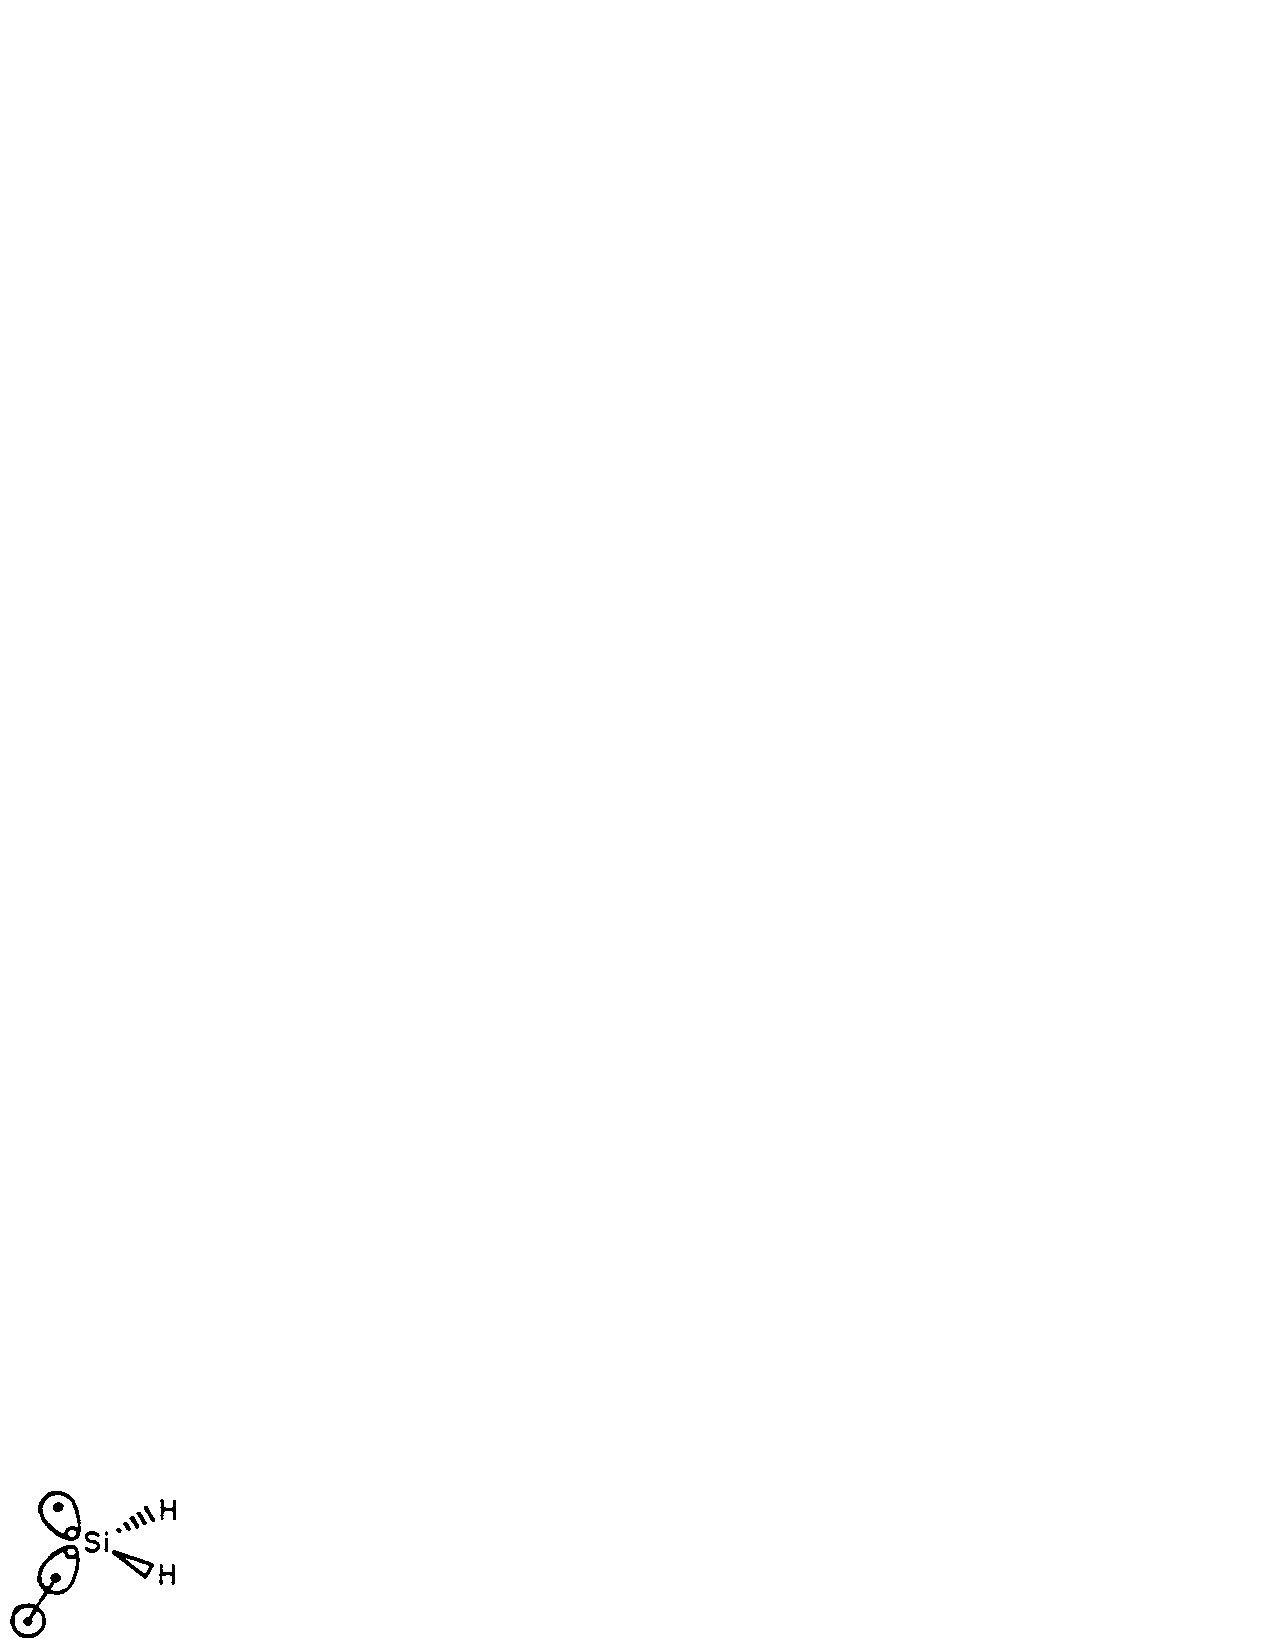
\includegraphics[scale=0.75]{fig6-04b}
\label{chap6-eqno15}
\end{equation}
Allowing all of the orbitals to readjust leads to three equivalent
bond pairs, each having the character expected for the average of two
$p$ bonds and one lobe bond. Averaging the bond angles ($92^\circ$, 
$119.4^\circ$, and $119.4^\circ$) leads to a predicted bond angle of 
$110.3^\circ$ for SiH$_3$. The actual bond angle in SiH$_3$ is
$110.6^\circ$.  The optimum orbitals are shown in Figure
\ref{chap6-fig5-2}. 

\begin{figure}
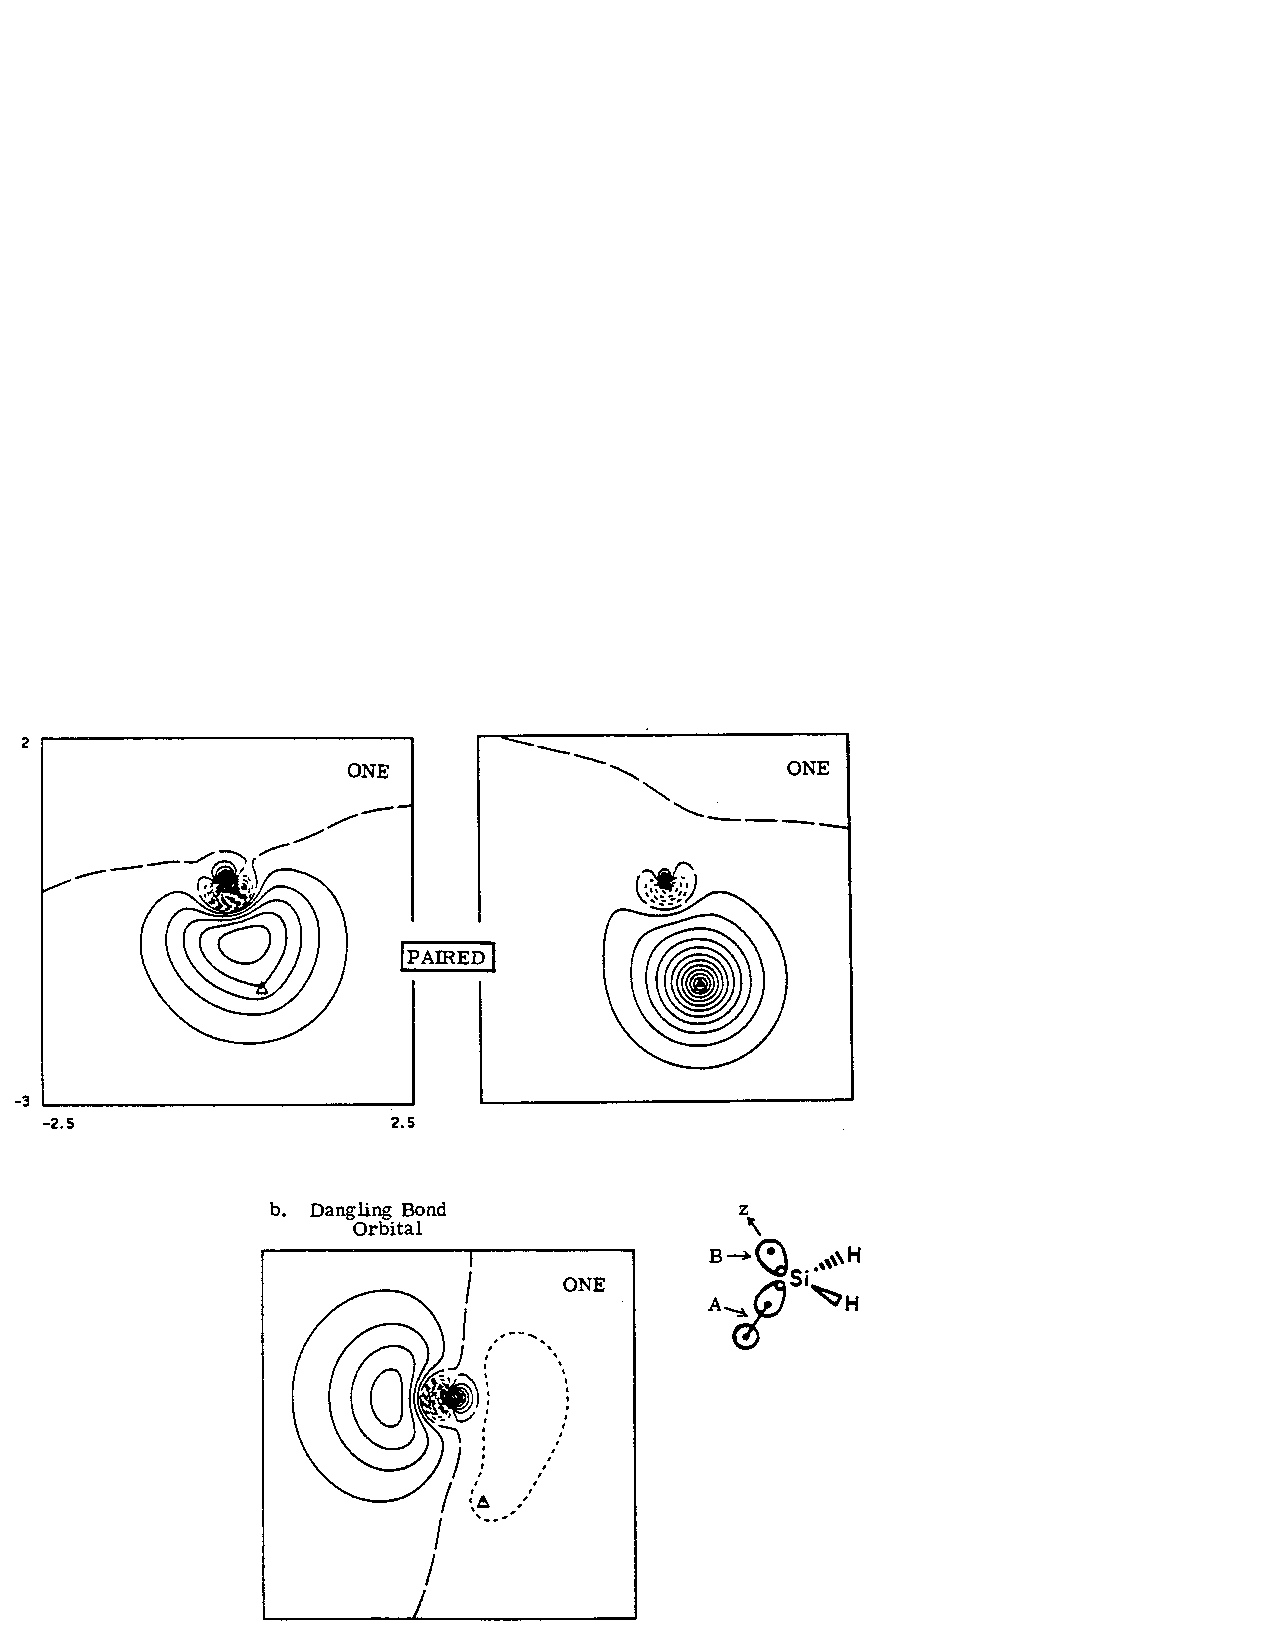
\includegraphics[scale=0.75]{fig6-06}
\caption{GVB orbitals for SiH$_3$}
\label{chap6-fig5-2}
\end{figure}

It is important to note that the ground states of SiH and SiH$_2$
resulted from bonding to $p$ orbitals and did not involve unpairing
the two lobe orbitals of Si. In order to bond an H to SiH$_2$,
however, it is necessary to unpair the lobe orbitals, and therefore we
expect the H$_2$Si-H bond energy to be significantly weaker than the
HSi-H energy.

Consider now how the character of the SiH$_3$ wavefunction changes as
the molecule is diestored to a planar geometry. The nonbonding lobe
orbital must remain orthogonal to the bond pairs and thus this orbital
becomes a $p\pi$ orbital at the planar geometry,
\begin{equation}
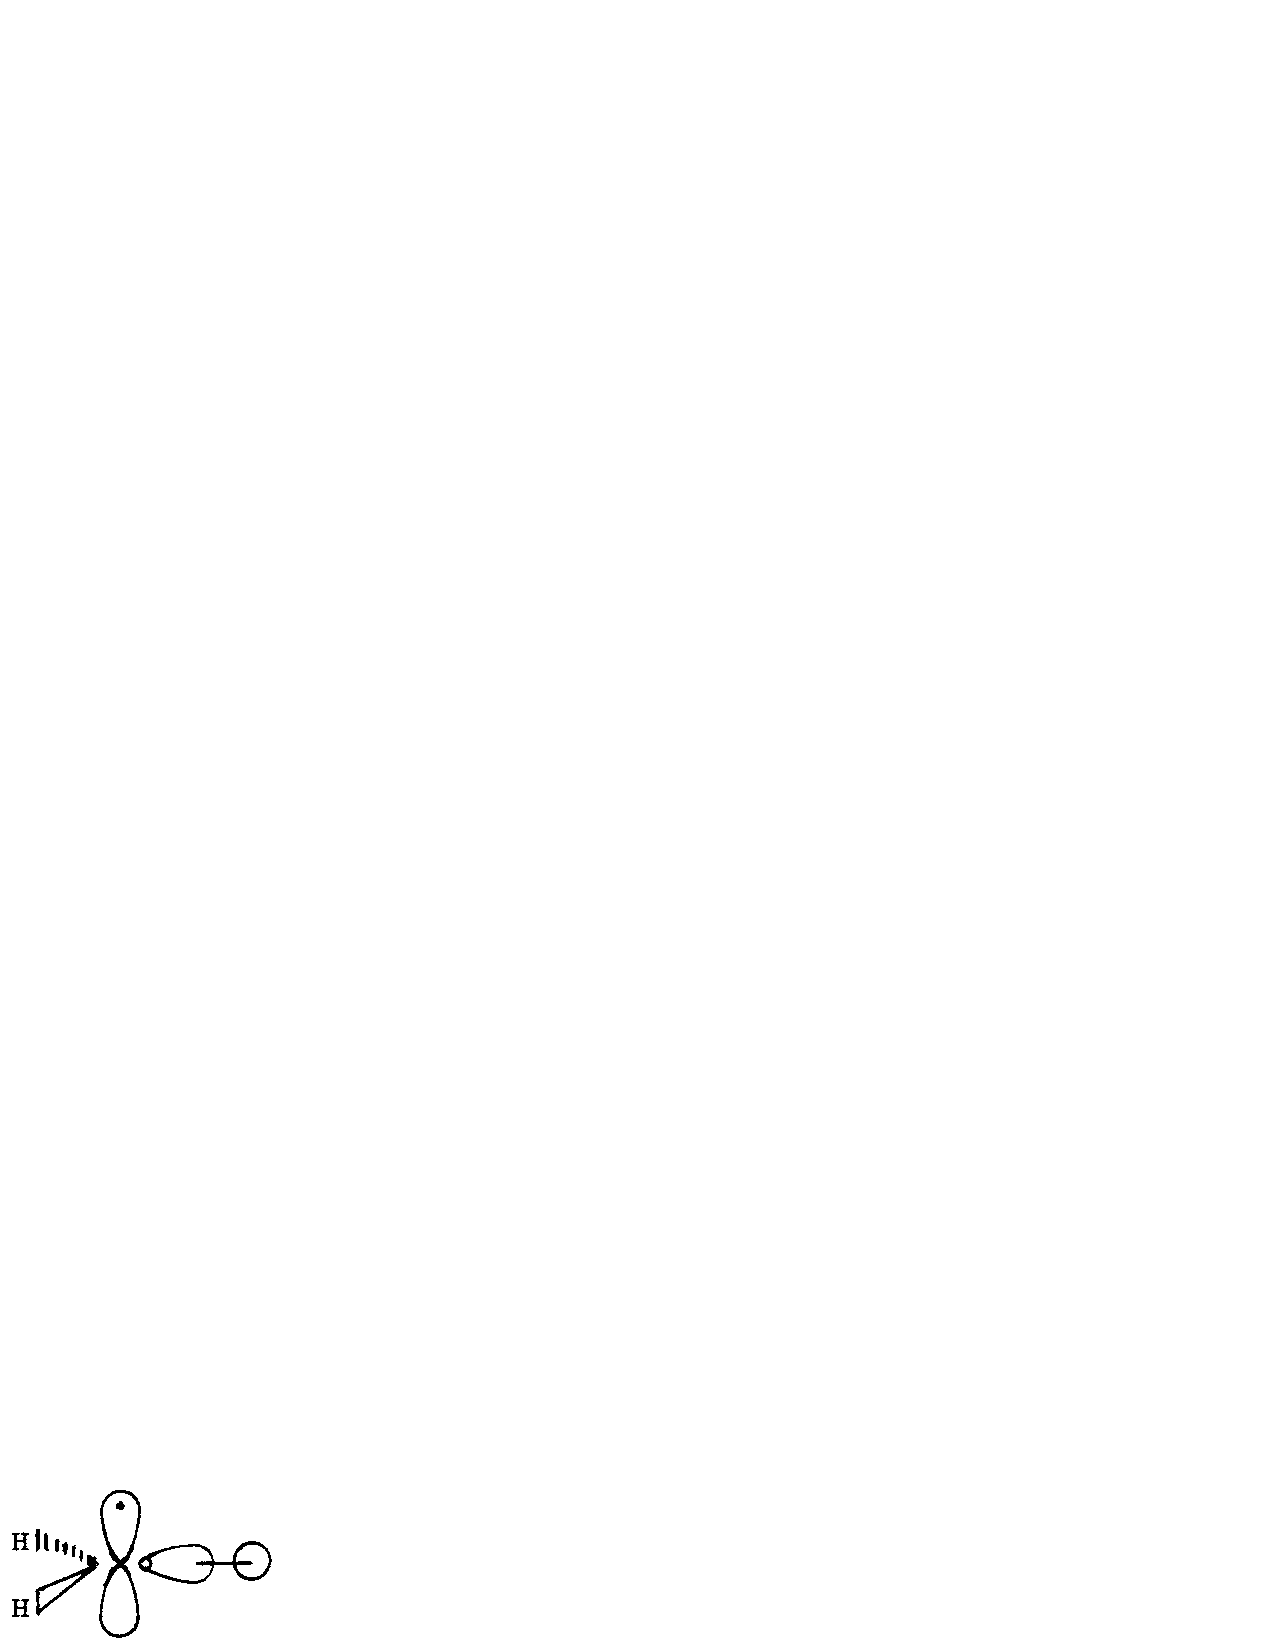
\includegraphics[scale=0.75]{fig6-05a}
\label{chap6-eqno15-2}
\end{equation}
Alternatively, the planar state can be considered to arise from
bonding two hydrogens to the lobe orbitals of the $^2\Pi$ state of
SiH, 
\begin{equation}
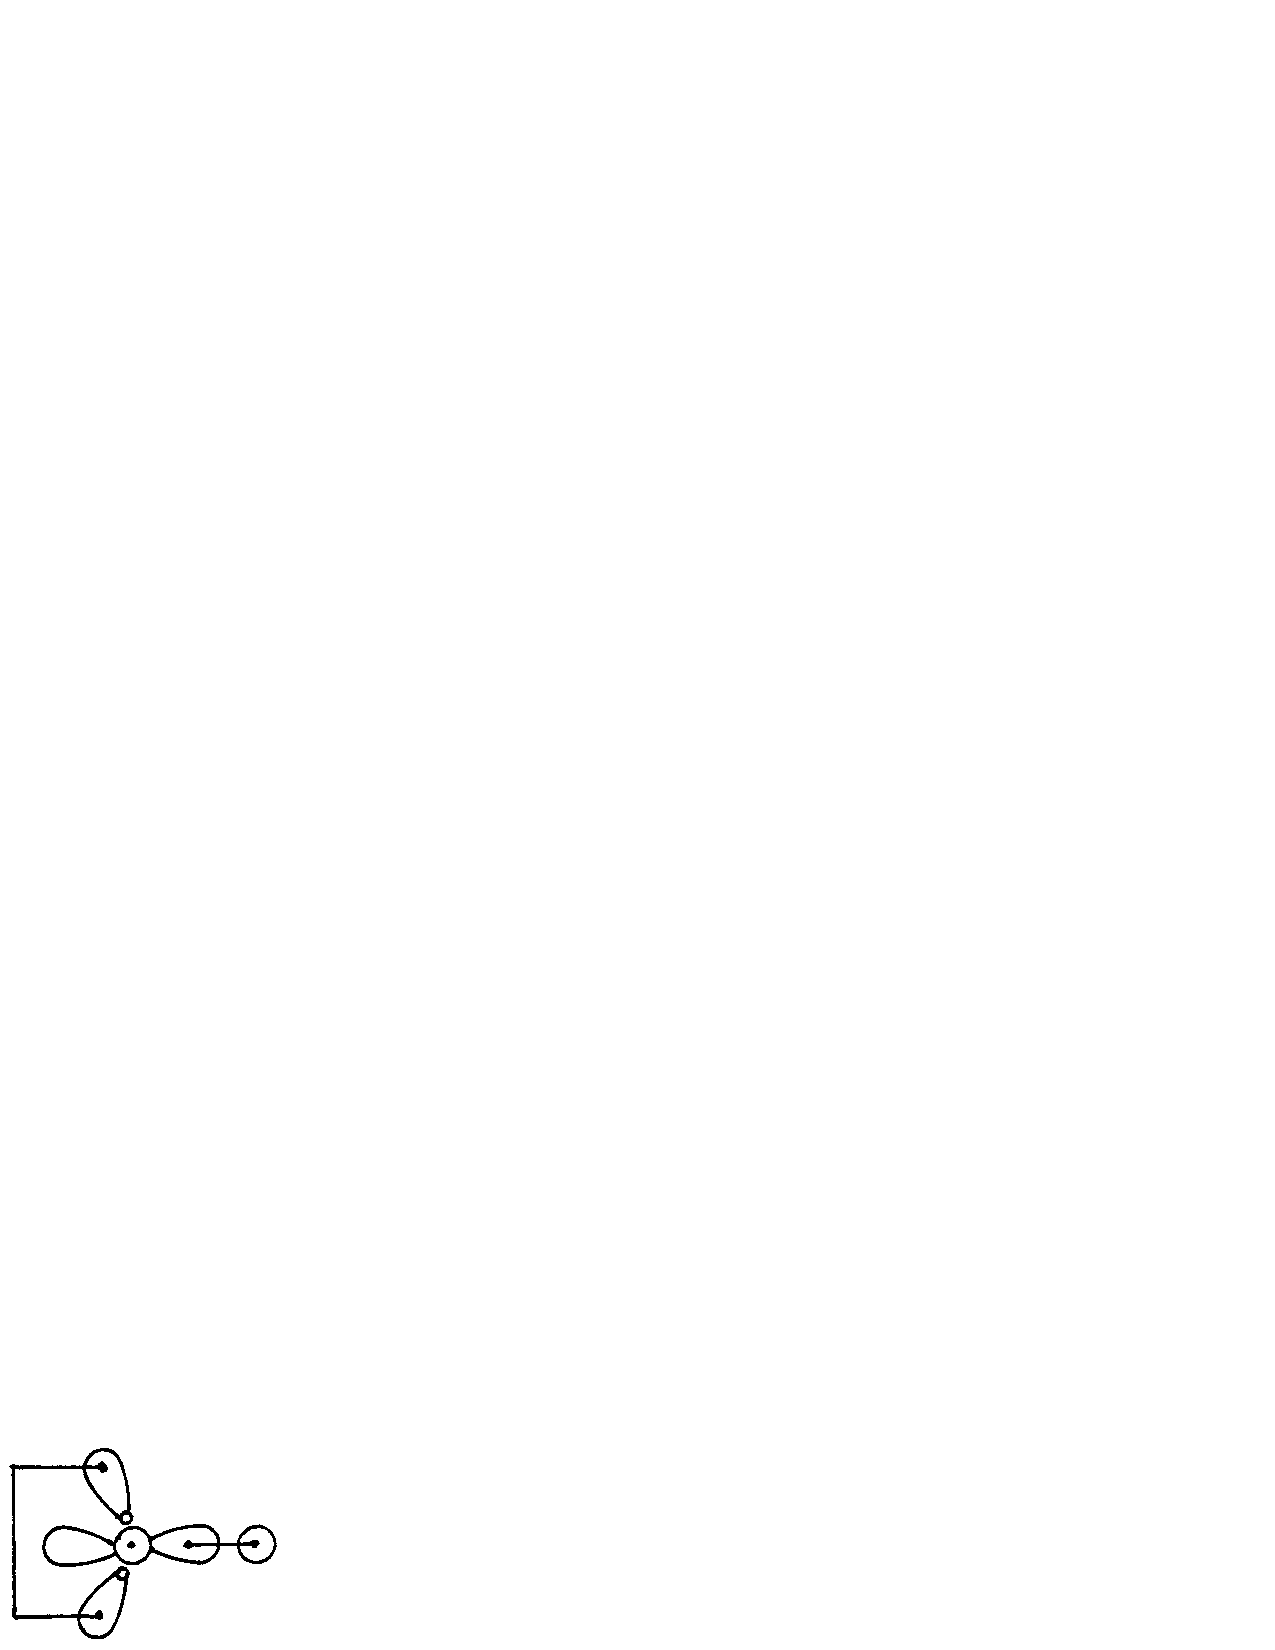
\includegraphics[scale=0.75]{fig6-05b}
\rightarrow
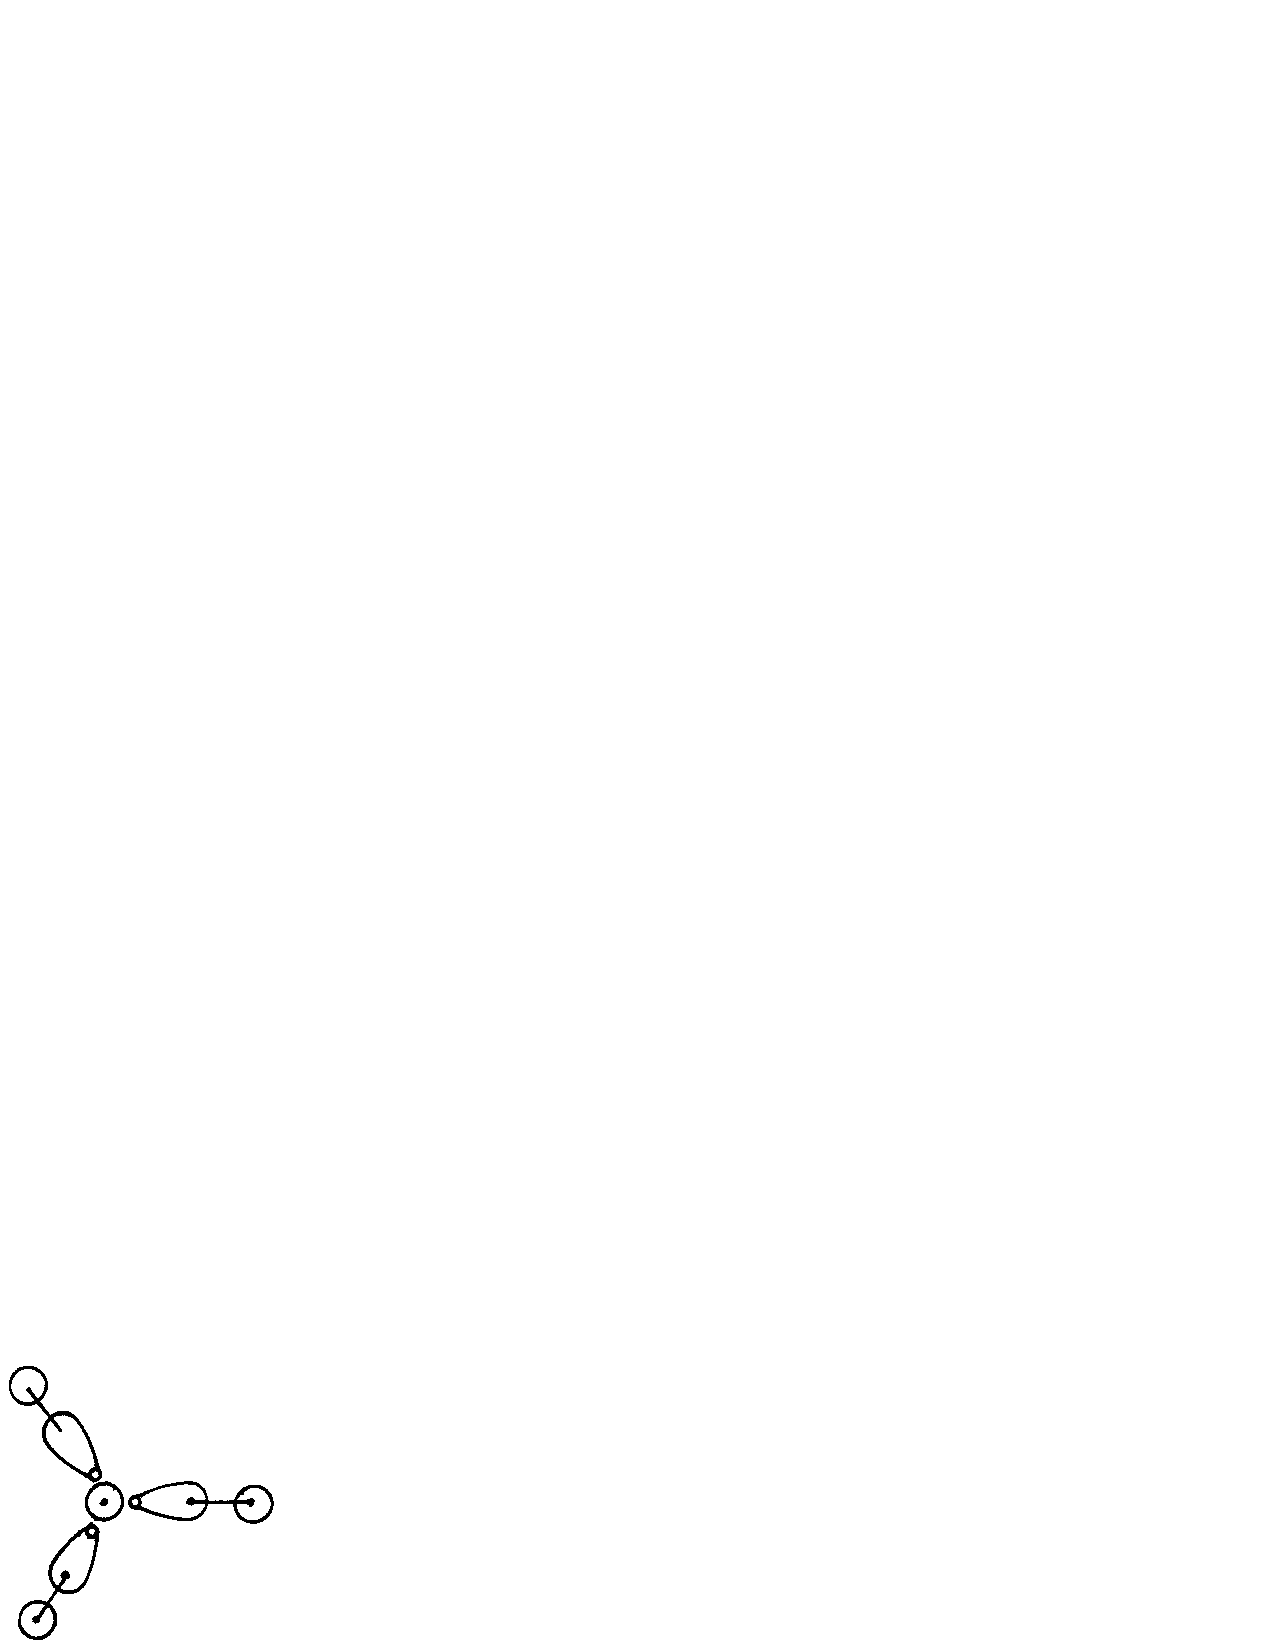
\includegraphics[scale=0.75]{fig6-05c}
\label{chap6-eqno15-3}
\end{equation}
The bond pairs, of course, readjust to become equivalent, and thus, 
each are roughly the average of two lobe bonds and one $p$ bond.  As 
discussed previously, the pyramidal molecule involves two $p$ bonds 
and one lobe bond.  Thus, the barrier to inversion, approximately 21 
kcal in SiH$_3$, is directly related to the difference between $p$ 
bonds and lobe bonds.

Starting with (\ref{chap6-eqno15}) and bonding an H to the unpaired
lobe orbital, leads to tetrahedral SiH$_4$.  Again, all the bond pairs
readjust to minimize bond-bond repulsions and to maximize bonding
interactions, resulting in four equivalent bond pairs.  The optimum
orbitals are shown in Figure \ref{chap6-fig6}.

\begin{figure}
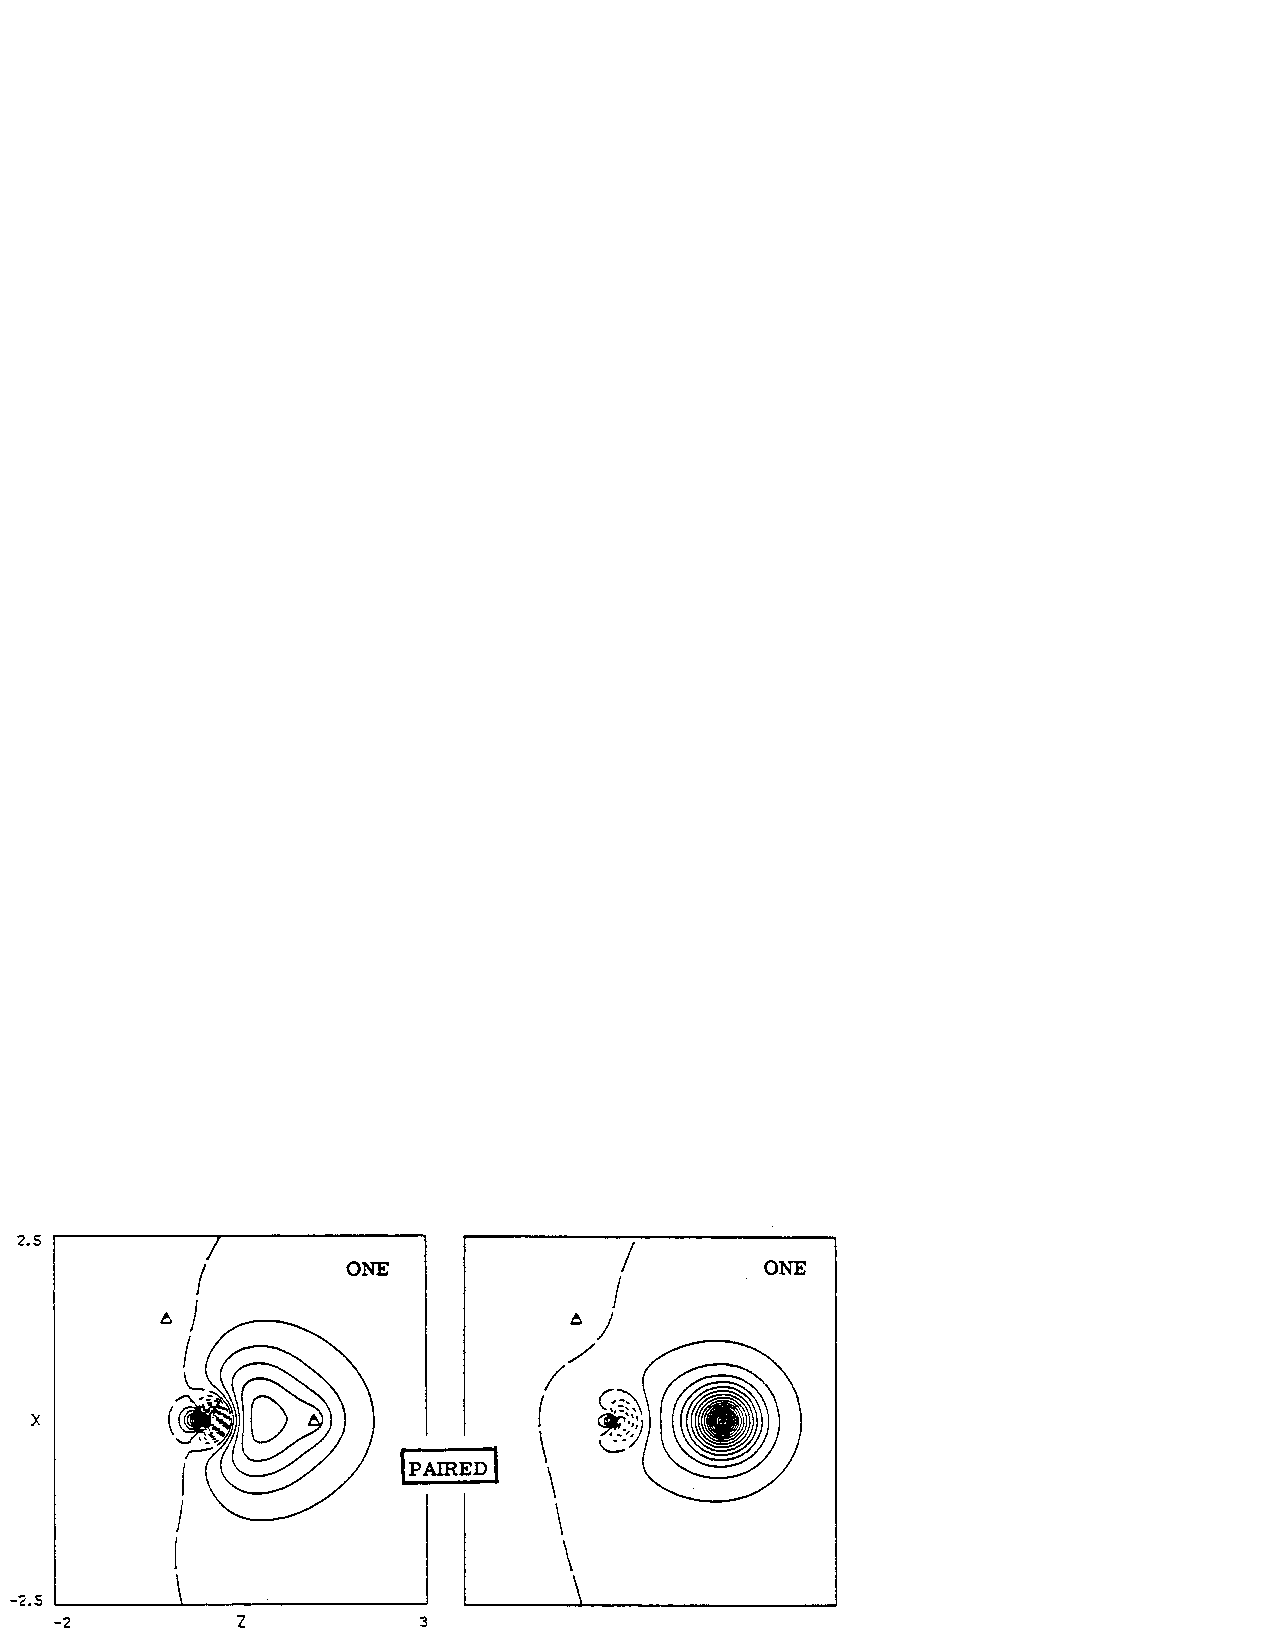
\includegraphics[scale=0.75]{fig6-06a}
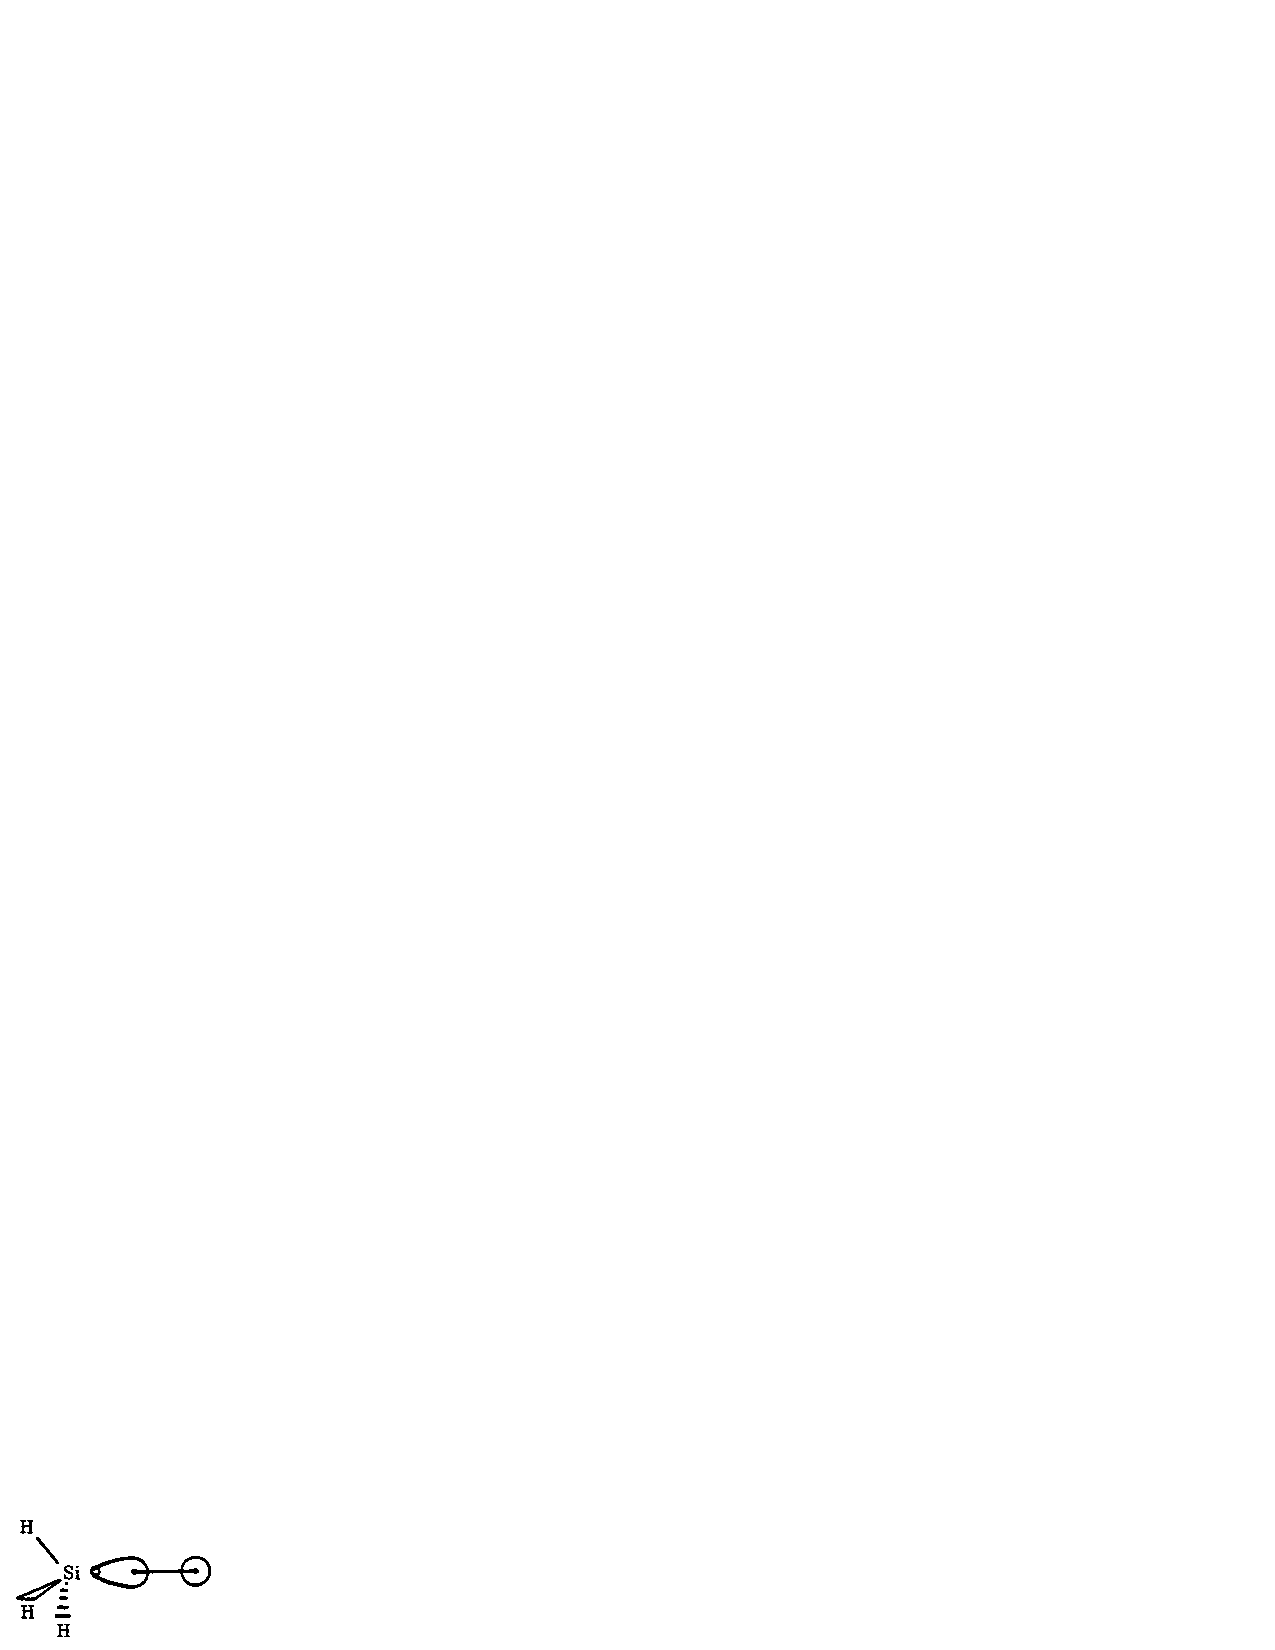
\includegraphics[scale=0.75]{fig6-06b}
\caption{GVB orbitals for SiH$_4$.}
\label{chap6-fig6}
\end{figure}

\subsection{Summary}

In the preceding discussion, we constructed the lowest states of 
SiH$_n$ by bonding a hydrogen atom to the ground state of 
SiH$_{n-1}$.  In this model we, first, assumed that the orbitals of 
SiH$_{n-1}$ remain unperturbed by the additional hydrogen.  Second, 
after deciding on the optimal orbital pairing and geometry, we allowed 
for slight readjustments of the various orbitals.

A key feature in this qualitative description of SiH$_n$, is the use of 
optimized GVB orbitals, allowing a consistent, 
progressive description of each state.  In the GVB 
description, the correlated orbitals are hydridized even in the atom, 
and these orbitals are found to change quite continuously, as a 
function of the number of bonds.  With this simple model, we were able 
to understand that:
\begin{enumerate}
\item the ground state of SiH should be a 
${^2\Pi}$ state and there should be a low-lying ${^4\Sigma}^-$ 
excited state,  
\item SiH$_2$ should also have two low-lying states, 
a ${^1A}_1$ ground state of bond angle of approximately 
117$^{\circ}$, 
\item SiH$_3$ should be pyramidal with a large 
barrier, 21 kcal, for inversion.
\item the smallest bond energy 
in the series $D_{H-SiH_{n-1}}$ should be $D_{H-SiH_2}$, since only in 
making this bond is it necessary to unpair the Si lobe orbitals.
\end{enumerate}

\section{Second-Row Atoms}

From the previous section, it is clear that the character of the 
atomic ground state wavefunctions, plays a dominant role in molecular 
bonding.  In this section, we will briefly discuss the ground states 
of the other second-row atoms, Na-Ar, as a prelude to a consideraton 
of the hydrides of these atoms.

Again, ignoring the core electrons, the ground state atoms have the 
following HF configurations.  
\begin{equation}
\begin{array}{lll}
\mathrm{Na} & (3s)^1 & 
{\cal A} \left[ \left( \phi_s \right) \alpha \right] = 
{\cal A} \left[ \phi_{3s} \alpha \right] \\
\mathrm{Mg} & (3s)^2 &
{\cal A} \left[ \left( \phi_s \right)^2 \alpha \beta 
\right] = {\cal A} \left[ \left( \phi_{3s} \alpha \right) 
\left( \phi_{3s} \beta \right) \right] \\
\mathrm{Al} & (3s)^2 (3p)^1 &
{\cal A} \left[ ( \phi_s )^2 \left( \phi_{p_z} 
\right) \alpha \beta \alpha \right] \\
\mathrm{Si} & (3s)^2 (3p)^2 &
{\cal A} \left[ \left( \phi_s \right)^2 \left( 
\phi_{p_z} \right) \left( \phi_{p_y} \right) \alpha \beta \alpha 
\alpha \right] \\
\mathrm{P} &(3s)^2 (3p)^3 &
{\cal A} \left[ \left( \phi_s \right)^2 \left( 
\phi_{p_z} \right) \left( \phi_{p_y} \right) \left( \phi_{p_x} 
\right) \alpha \beta \alpha \alpha \alpha \right]\\
\mathrm{S} & (3s)^2 (3p)^4 &
{\cal A} \left[ \left( \phi_s \right)^2 \left( 
\phi_{p_z} \right)^2 \left( \phi_{p_y} \right) \left( \phi_{p_x} 
\right) \alpha \beta \alpha \beta \alpha \alpha \right] \\
\mathrm{Cl} & (3s)^2 (3p)^5 &
 {\cal A} \left[ \left( \phi_s \right)^2 \left( 
\phi_{p_z} \right)^2 \left( \phi_{p_y} \right)^2 \left( \phi_{p_x} 
\right) \alpha \beta \alpha \beta \alpha \beta \alpha \right] \\
\mathrm{Ar} & (3s)^2 (3p)^6 &
 {\cal A} \left[ \left( \phi_s \right)^2 \left( 
\phi_{p_z} \right)^2 \left( \phi_{p_y} \right)^2 \left( \phi_{p_x} 
\right) \alpha \beta \alpha \beta \alpha \beta \alpha \beta \alpha
\right] \\
\end{array}
\end{equation}

Correlating the $3s$ pair of P, in the same way as for Si, (4), leads 
to the wavefunction
\begin{eqnarray}
{\cal A} \left[ \left( \phi_{\ell} \phi_{\bar{\ell}} + 
\phi_{\bar{\ell}} \phi_{\ell} \right) \phi_{p_z} \phi_{p_y} 
\phi_{p_x} \alpha \beta \alpha \alpha \alpha \right] &=& {\cal A}| 
\left[ \left( \phi^2_s - \lambda^2 \phi^2_{p_x} \right) \phi_{p_z} 
\phi_{p_y} \phi_{p_x} \alpha \beta \alpha \alpha \alpha \right]\cr
&=& {\cal A} \left[ \phi^2_s \phi_{p_z} 
\phi_{p_y} \phi_{p_x} \alpha \beta \alpha \alpha \alpha \right]\cr
&& - \lambda^2 {\cal A} \left[ \phi^2_{p_x} \phi_{p_z} 
\phi_{p_y} \phi_{p_x} \alpha \beta \alpha \alpha \alpha 
\right]
\label{chap6-eqno16}
\end{eqnarray}
However, a second term of
\begin{equation}
{\cal A} \left[ \phi^2_{p_x} \phi_{p_z} 
\phi_{p_y} \phi_{p_x} \alpha \beta \alpha \alpha \alpha \right] ,
\end{equation}
has three electrons in the $\phi_{p_x}$ orbitals, and hence, in order
to satisfy the Pauli principle, this term must be zero.  (The second
term of (\ref{chap6-eqno16}) will be exactly zero only if the
correlating $\phi_{p_x}$ is identical to the singly-occupied
$\phi_{p_x}$.  In fact, these two orbitals will not be exactly equal,
and hence, there will be a small correlation effect.)  This will not,
however, change the qualitative description of bonding discussed here.
That is, since all three $3p$ orbitals are singly-occupied, the
GVB correlation of the $3s$ pair is eliminated,
and the GVB wavefunction of ground state P is
identical to the HF wavefunction.  Similarly for S, Cl, and
Ar, the ground state GVB and HF
wavefunctions are identical.

It should be noted here that we are considering only the dominant 
angular correlation involving $3p$ orbitals.  There are other less 
important correlations of the $3s$ pair, for example, radical 
correlation.  However, in Si the angular correlation leads to two lobe 
orbitals on opposite sides of the atom, allowing effective bonding to 
an H.  For P, S, Cl, and Ar, the radial correlation effects lead to 
no such separation, and hence, these correlation effects do not modify 
the qualitative description of the bonding.

In both Mg and Al, the GVB wavefunction leads to 
lobe orbitals just as for Si.  In Mg, since none of the $3p$ orbitals 
are occupied, the lobe pair can point in the $x$, $y$, or $z$ 
directions, leading to a GVB wavefunction of the 
form
\begin{equation}
{\cal A} \left[ \left( \phi^2_s - \lambda^2 \phi^2_{p_x} - \lambda^2 
\phi^2_{p_y} - \lambda^2 \phi_{p_z} \right) \alpha \beta \right].
\label{chap6-eqno17}
\end{equation}
For Al, the $3p_z$  orbital is singly-occupied, and hence, the lobe 
orbitals can point in only the $x$ or $y$ directions.  The resulting 
GVB wavefunction for ground state Al is
\begin{equation}
{\cal A} \left[ \left( \phi^2_s - \lambda^2 \phi^2_{p_x} - \lambda^2 
\phi^2_{p_y} \right) \phi_{p_z} \alpha \beta \alpha \right] .
\label{chap6-eqno18}
\end{equation}
For Na, with only one valence electron, there are no corresponding 
correlation effects.

\begin{figure}
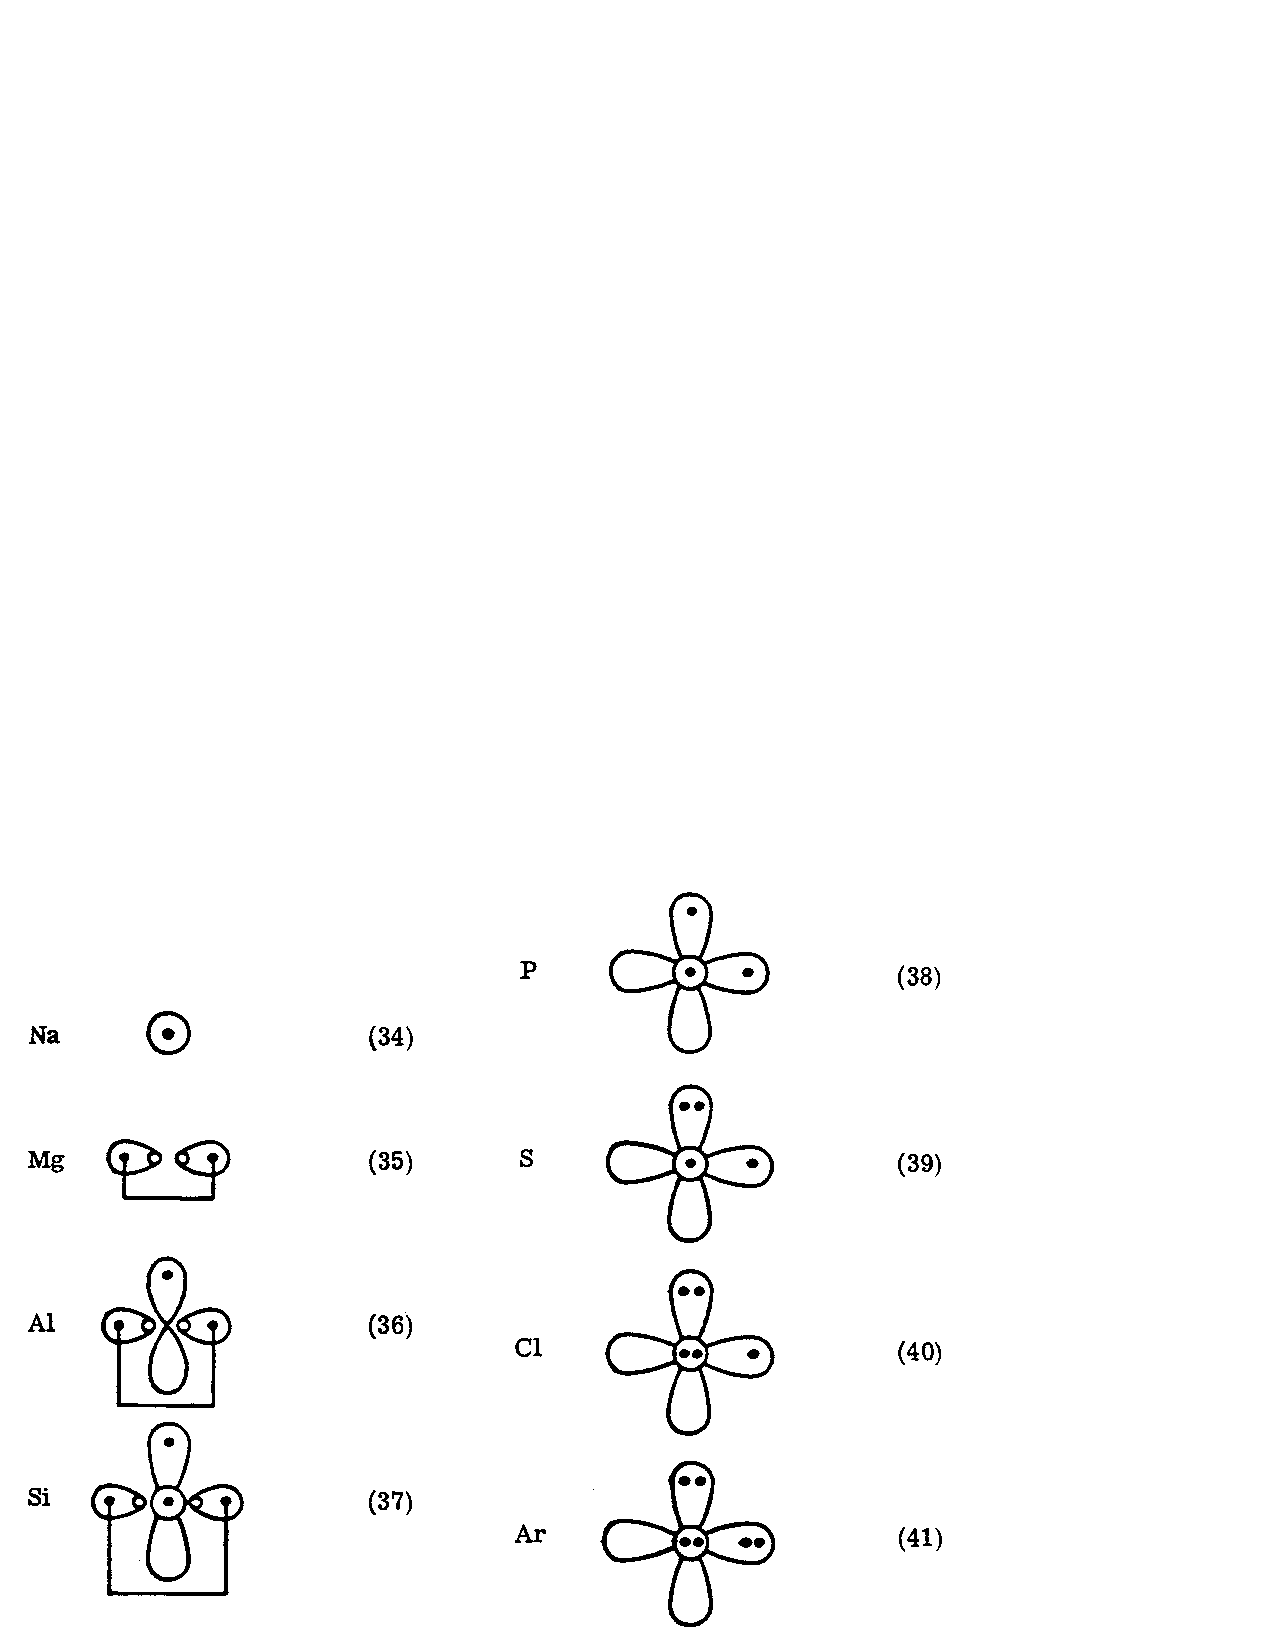
\includegraphics[scale=0.75]{fig6-06c}
\caption{}
\label{chap6-fig6-2}
\end{figure}

Schematically then, the simple GVB wavefunctions
of the second-row atoms are as shown in Figure \ref{chap6-fig6-2}.  As
before, a circle represents a $p$ orbital out of the plane for all
atoms except Na.  Note also that the $3s$ pair has been omitted for P,
S, Cl, and Ar.  For Mg and Al, the lobe pairs are actually correlated
in more than one direction, see (\ref{chap6-eqno17}) and
(\ref{chap6-eqno18}).  However, for simplicity in the diagrams, we
indicate only one of the possible correlations.  It is understood, in
these cases, that the actual GVB wavefunction is
a superposition of two or three such configurations incorporating $3s$
correlation into all unoccupied $p$ directions.

\section{Second-Row Hydrides}

\subsection{MgH$_n$}

Starting with the ground state of Mg and bonding an H to one of the
lobe orbitals, leads to the ground state $({^2\Sigma}^+)$ of MgH,
\begin{equation}
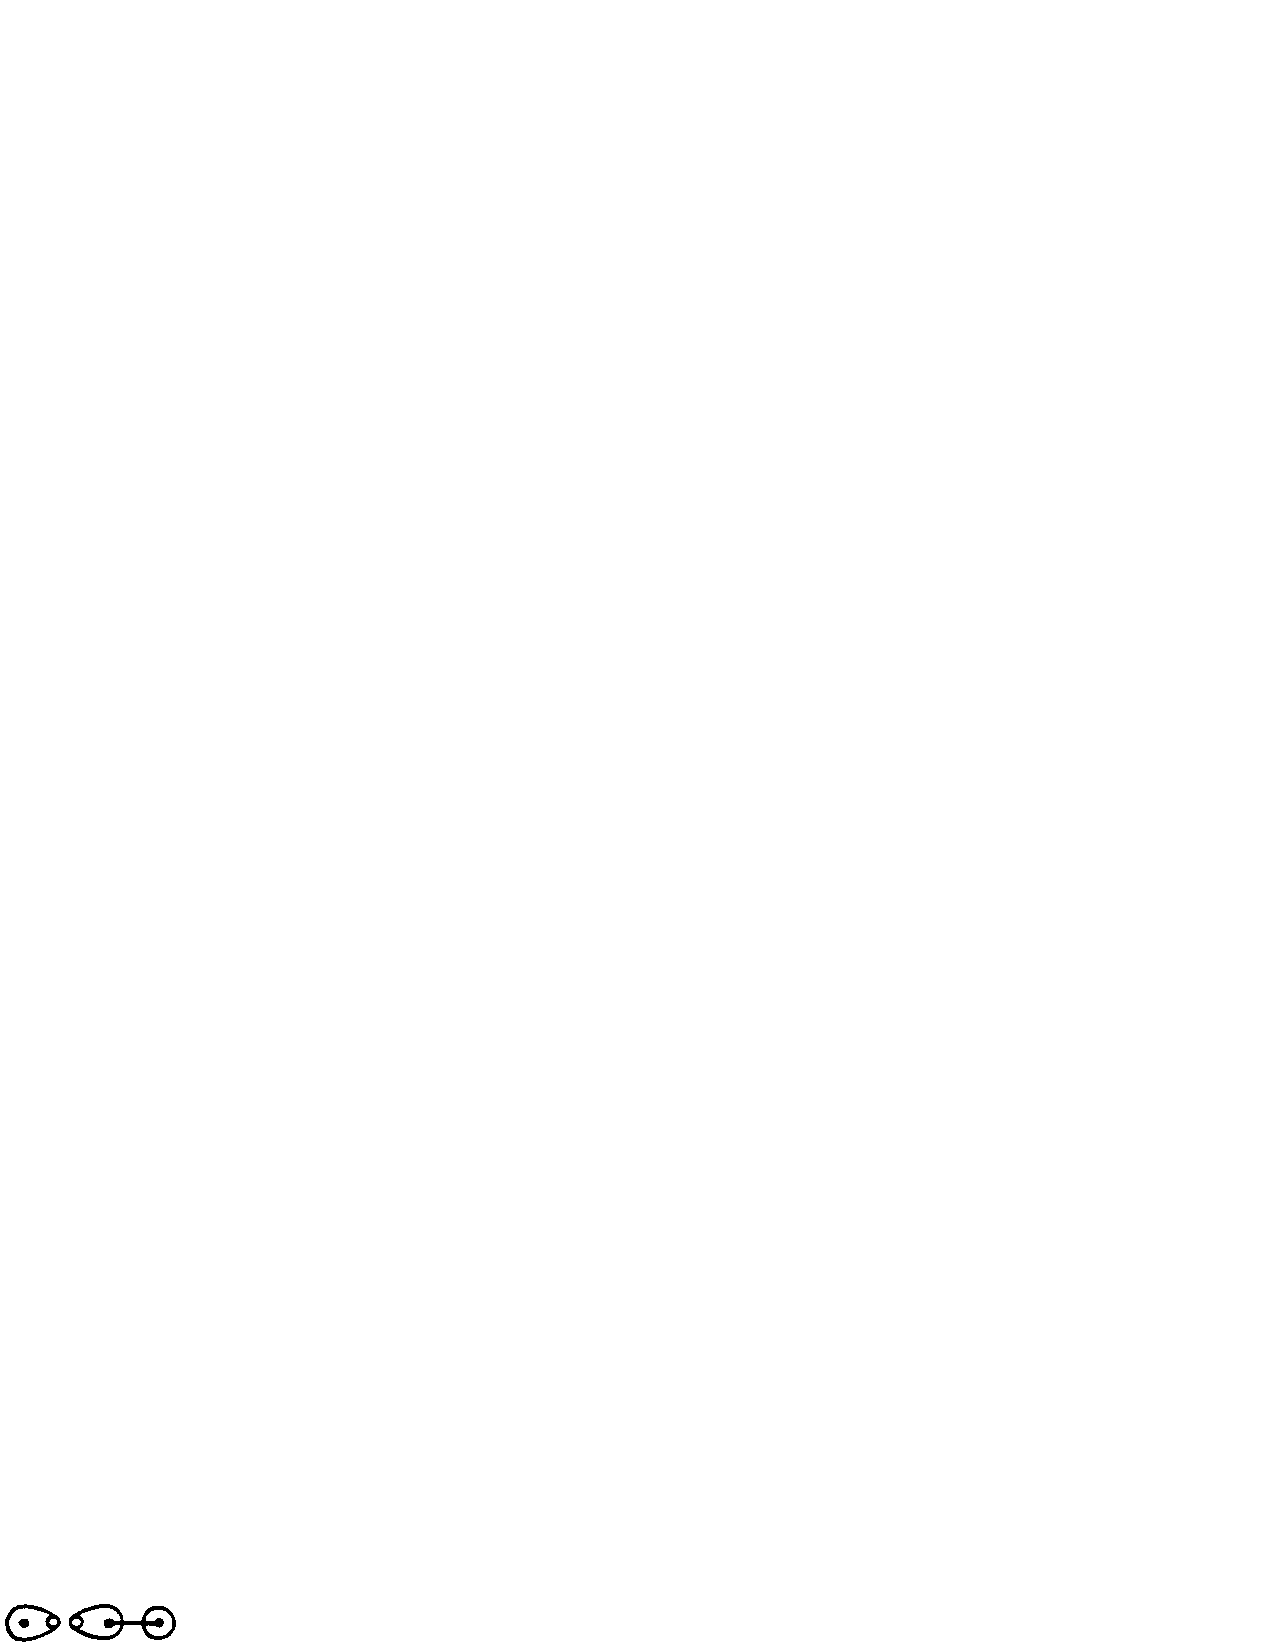
\includegraphics{fig6-06d}
\label{chap6-eqno20}
\end{equation}
Since this bonding scheme is the only one attainable with ground 
state Mg, there will be no other bound states of MgH dissociating to 
ground state atoms.

Similarly, the ground state of MgH$_2$ can be constructed by bonding 
an H to the unpaired lobe orbital of MgH.  The results is a linear
$({^1\Sigma}^+)$ ground states of
\begin{equation}
%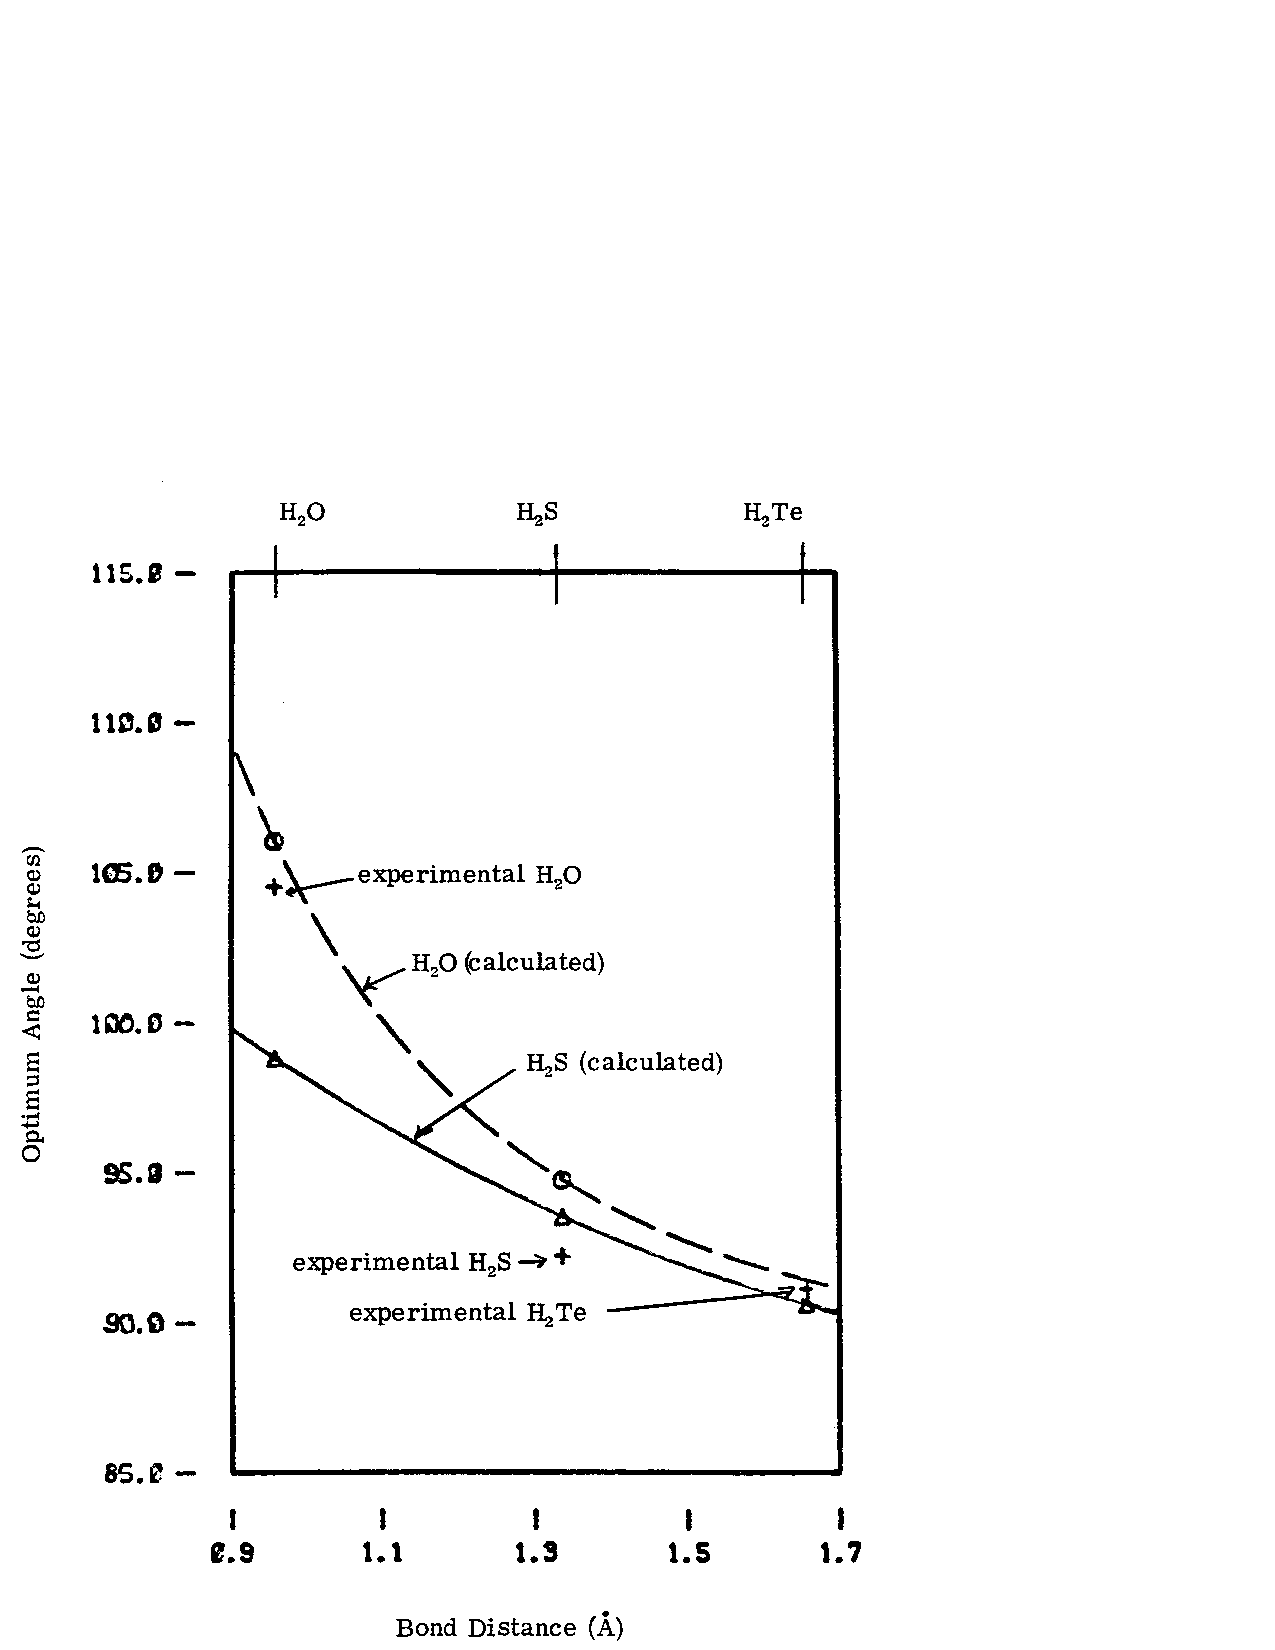
\includegraphics{fig6-06e}
\label{chap6-eqno21}
\end{equation}
Note that in making the first bond to Mg, it was necessary to unpair 
the Mg lobe orbitals.  Since the lobe orbitals overlap, unpairing them 
results in a significant increase in the total energy, 62 kcal, for 
the free atom.  The second MgH bond, however, is to an already 
unpaired lobe, and hence, the second bond should be much stronger 
than the first, i.e.
\begin{equation}
D_\mathrm{HMg-H} \ll D_\mathrm{Mg-H} .
\end{equation}
Consider MgH$_2$, (\ref{chap6-eqno21}), there are no more occupied
orbitals available for bonding, and therefore, MgH$_3$ will not be
bound.  van der Waals interactions can lead to a weak bond, $\leq$ 2
kcal, but we ignore such second-order effects here.

\subsection{Low-Lying States of AlH$_n$}

Starting with the ground state of Al, (\ref{chap6-eqno20}), an H can
bond either to the singly-occupied $p$ orbital, leading to the
$({^1\Sigma}^+)$ state
\begin{equation}
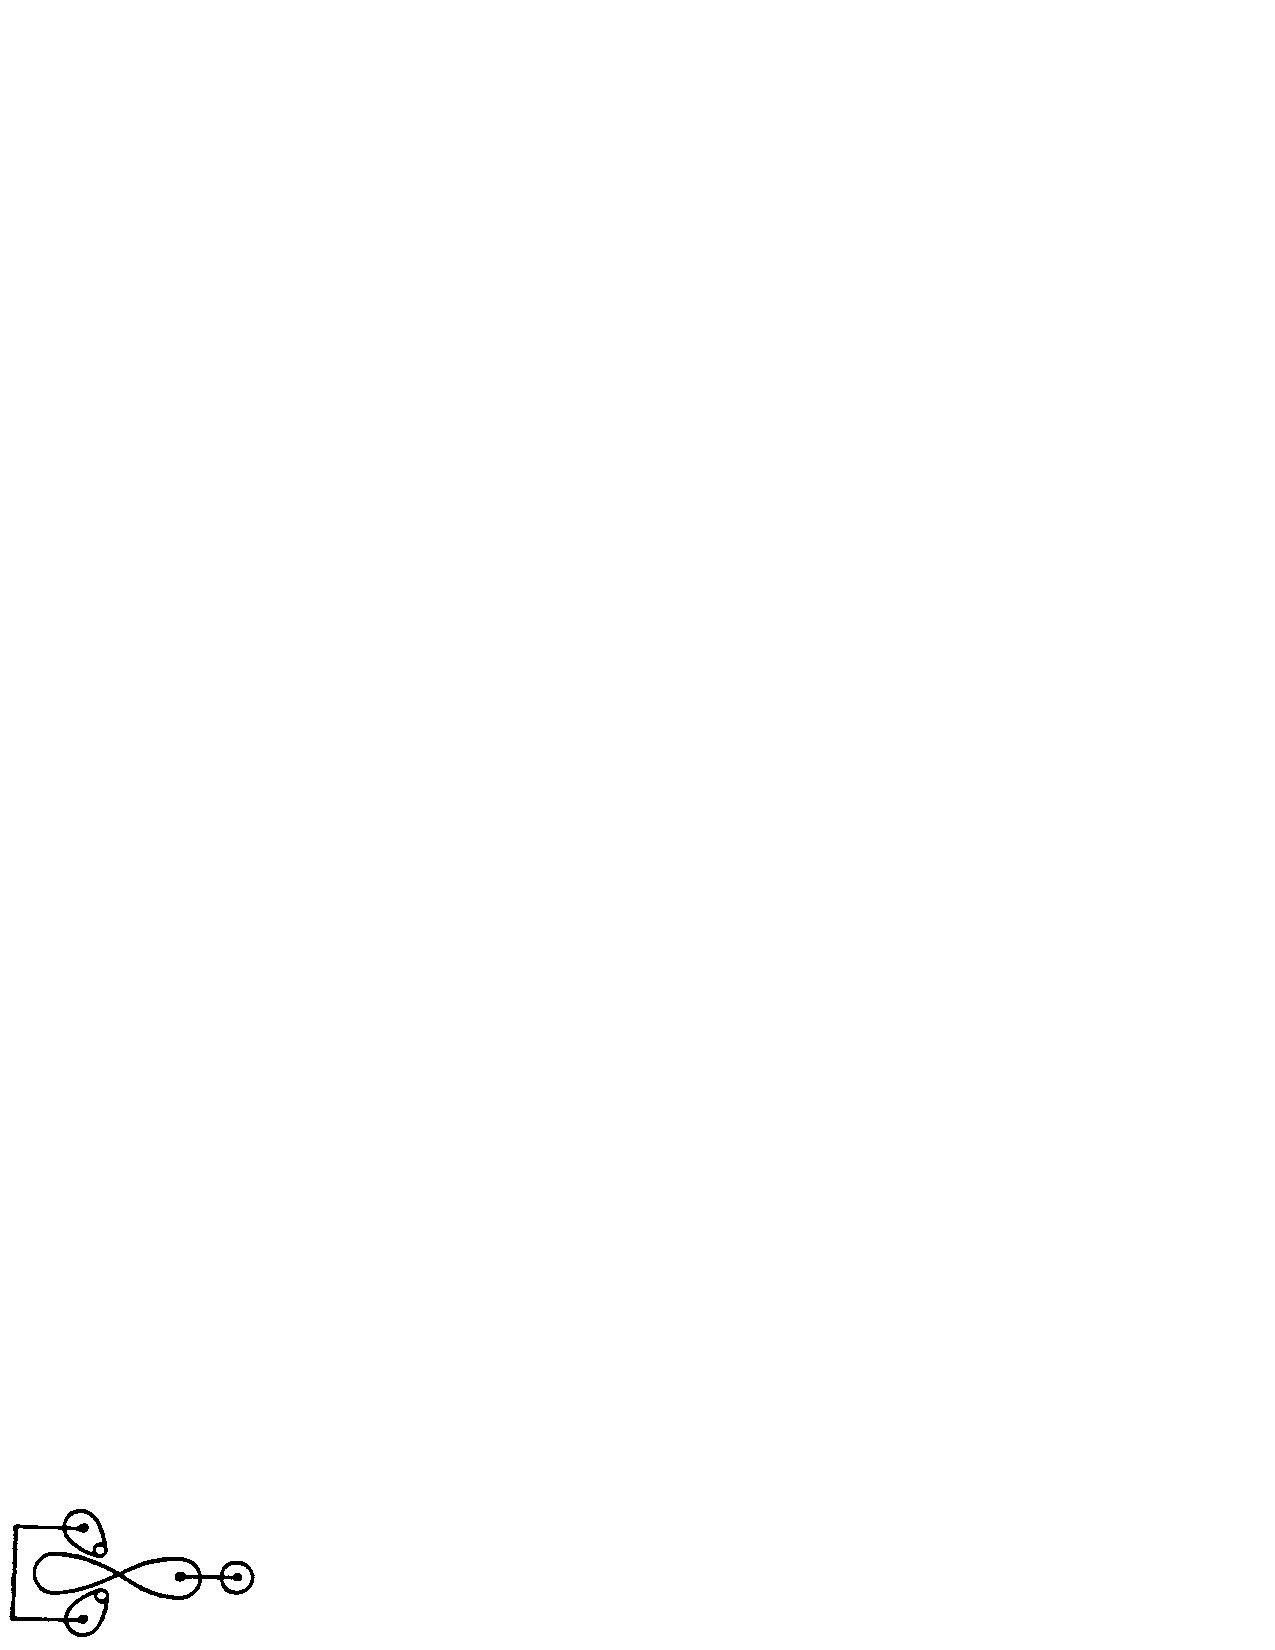
\includegraphics{fig6-06f}
\label{chap6-eqno22}
\end{equation}
or to one of the lobe orbitals, leading to the ${^3\Pi}$ state,
\begin{equation}
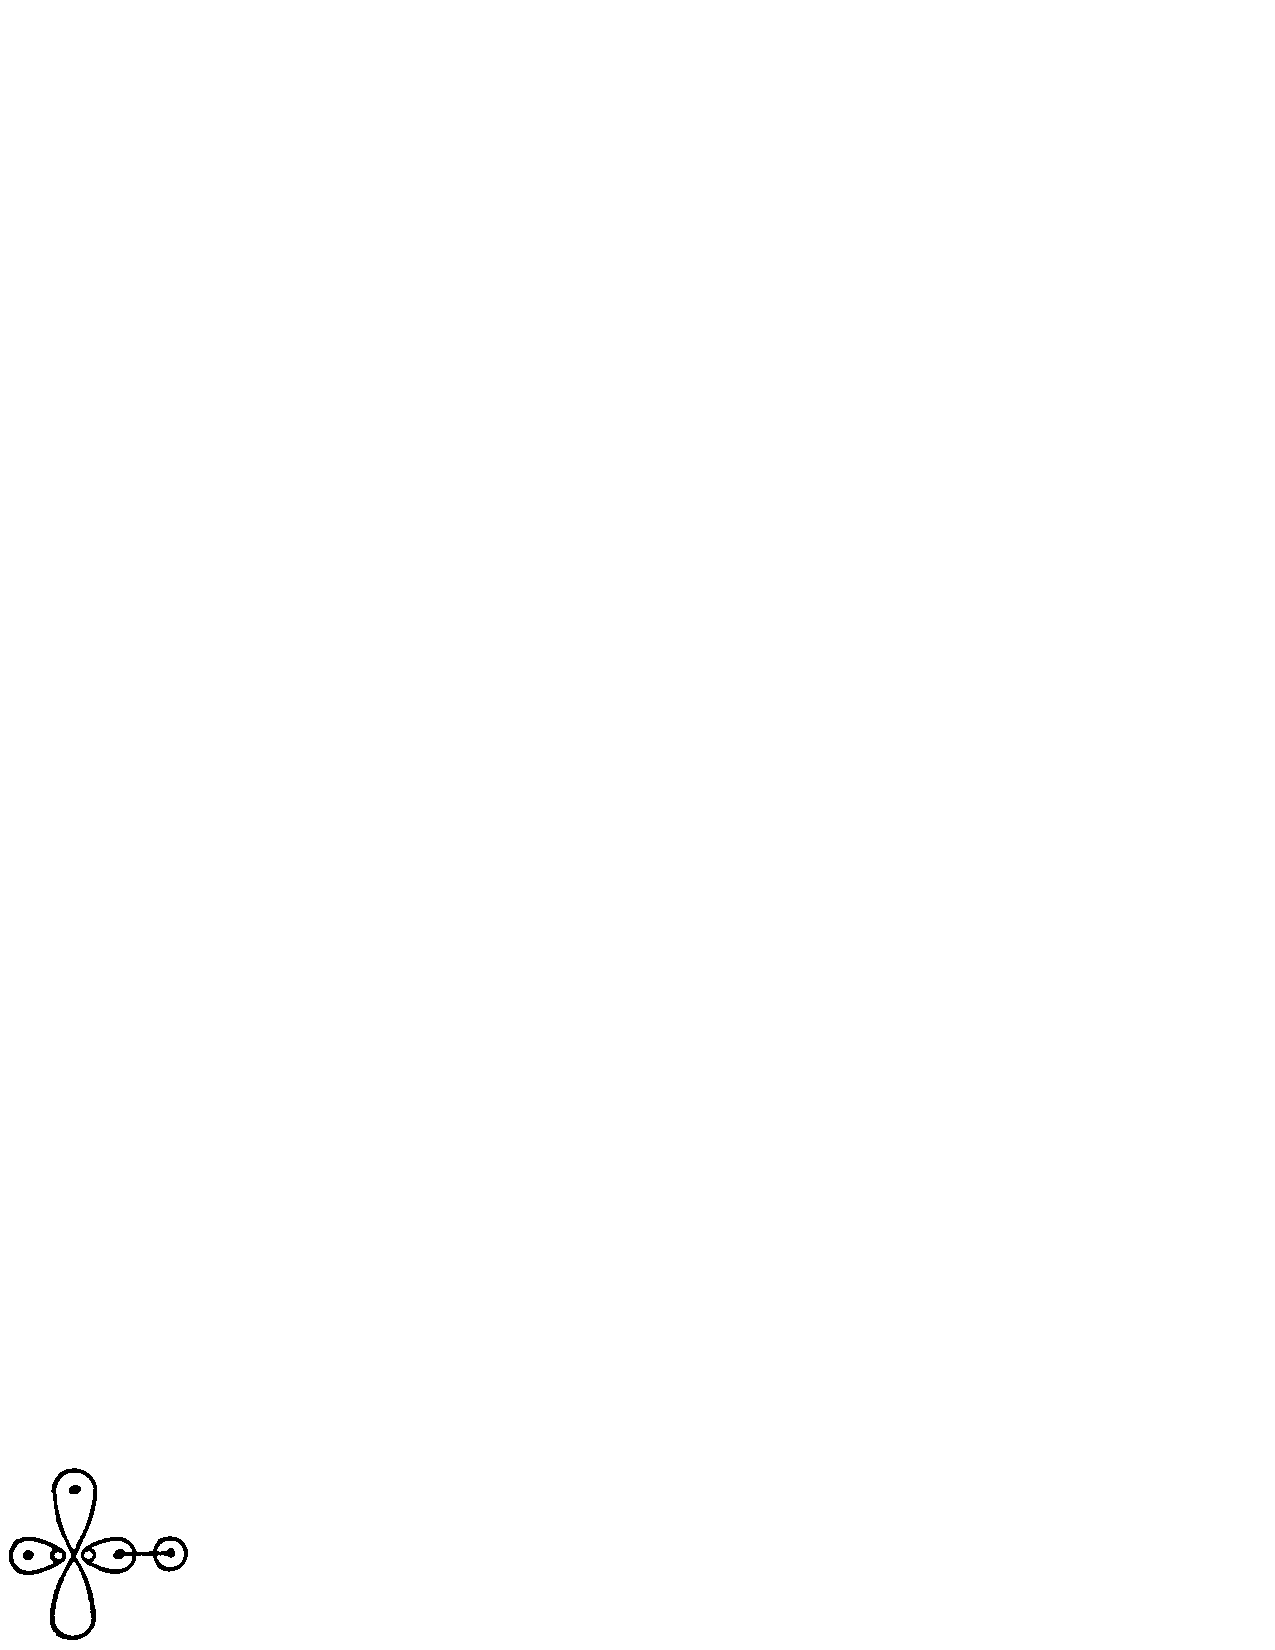
\includegraphics{fig6-06g}
\label{chap6-eqno22-2}
\end{equation}
As with Si, the bond to the unpaired $p$ orbital will be stronger than
the bond to a lobe orbital, and hence, the ground state of AlH is the
$({^1\Sigma}^+)$ state.  As with Si, interactions between the bond
pair and the lobe pair in (\ref{chap6-eqno22}) result in the lobe
orbitals bending back to an angle of approximately 128$^{\circ}$ with
respect to the bond axis.

Consider the ground state of AlH, the only orbitals available for
bonding are the lobes.  Bonding a hydrogen to one of the lobe orbitals
of (\ref{chap6-eqno22}), leads to
\begin{equation}
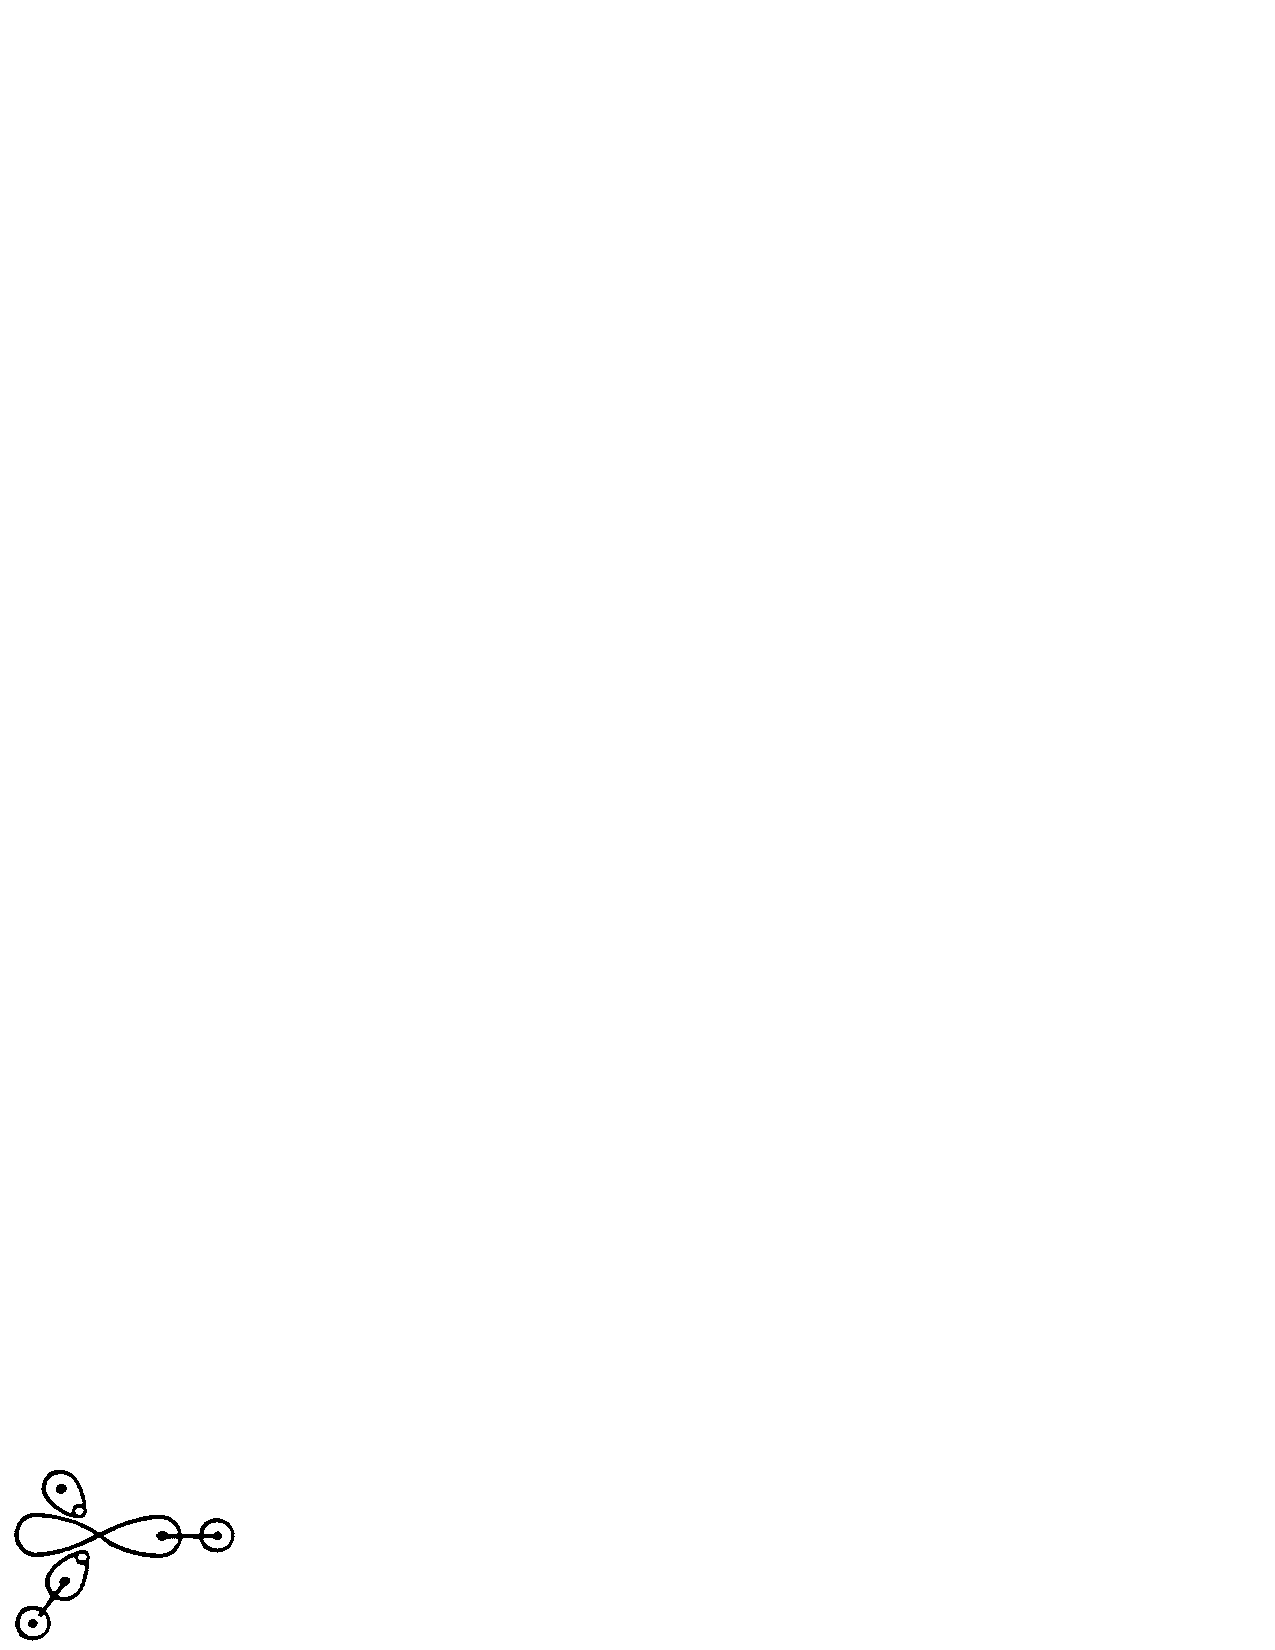
\includegraphics{fig6-06h}
\label{chap6-eqno23}
\end{equation}
and allowing the bond to readjust, see (\ref{chap6-eqno13}) and
(\ref{chap6-eqno14}) for SiH$_2$, leads to the ${^2A}_1$ state of
AlH$_2$,
\begin{equation}
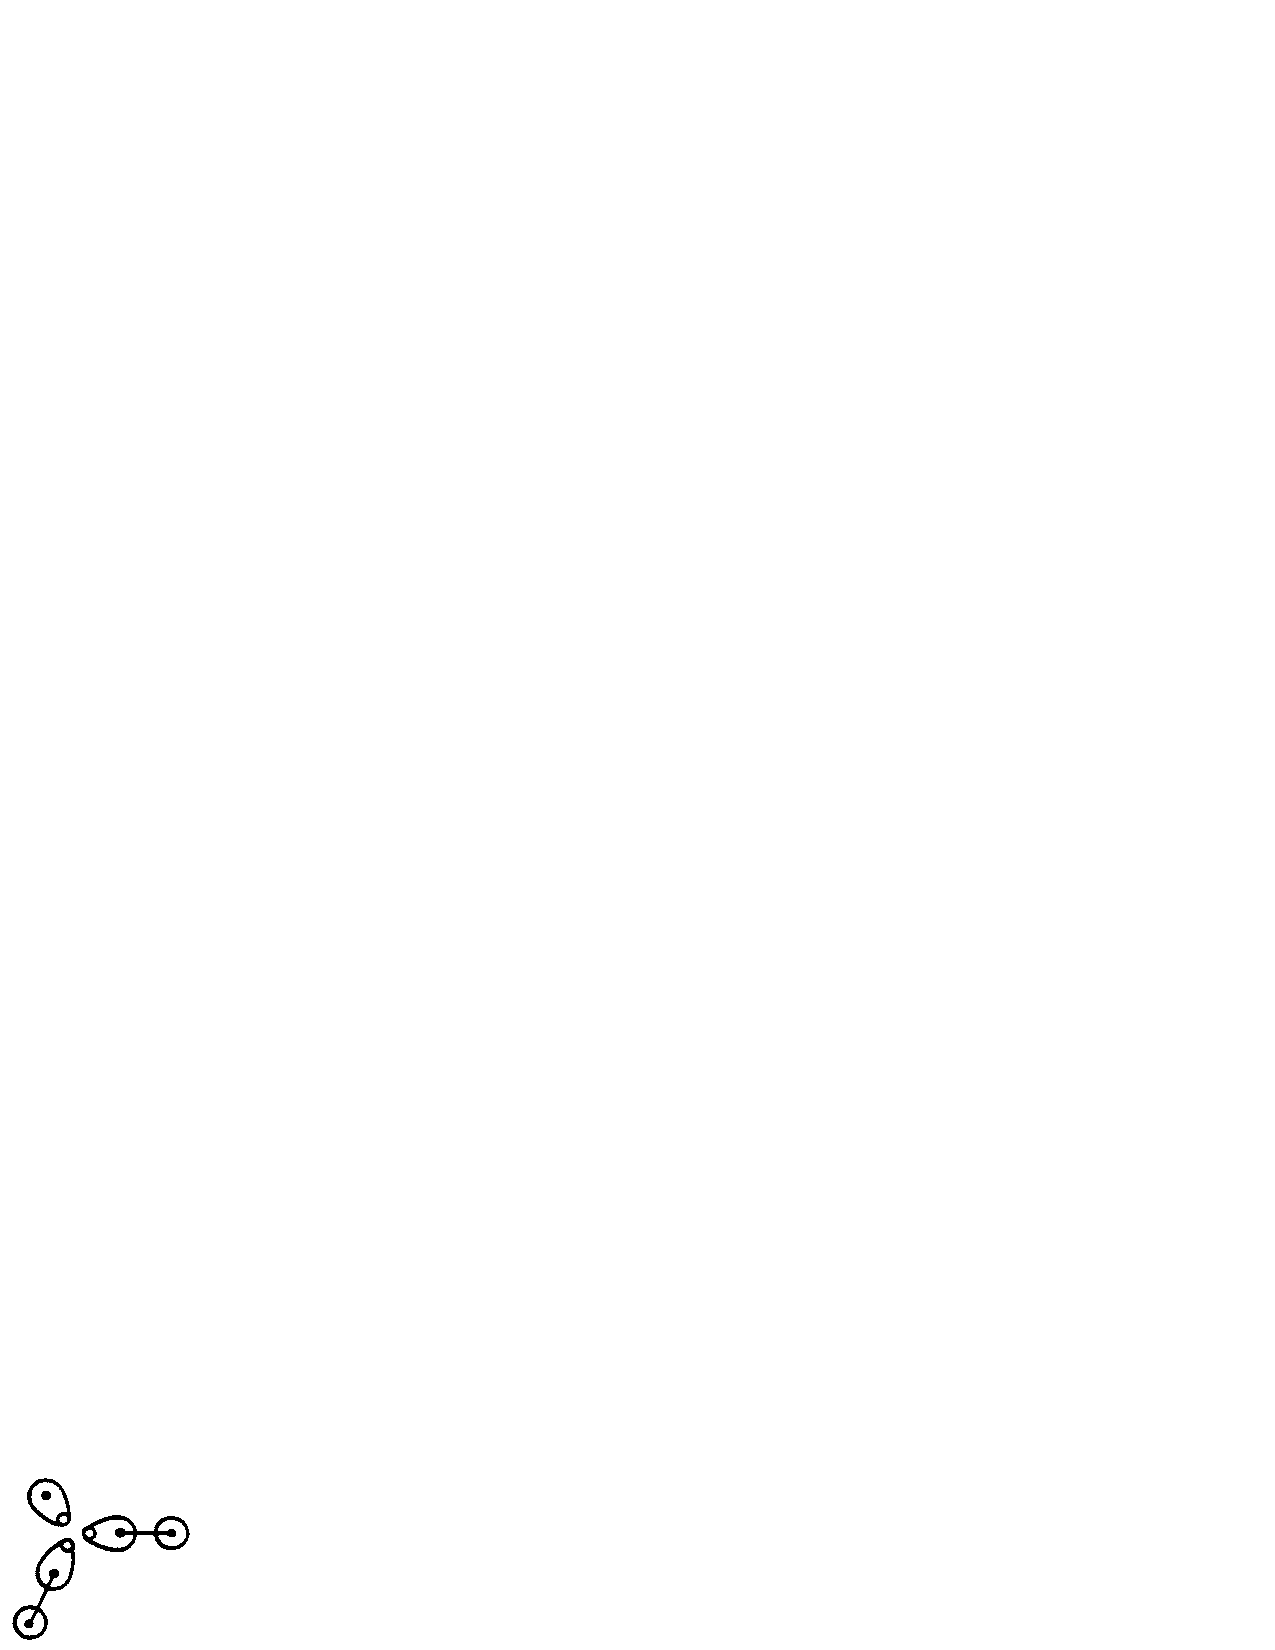
\includegraphics{fig6-06i}
\end{equation}
As in SiH$_2$, Pauli principle repulsions between the two bond pairs 
and the singly-occupied lobe orbital, will decrease the AlH$_2$ angle 
from 128$^{\circ}$, to approximatley 117$^{\circ}$, the lobe-bond 
angle of AlH, (\ref{chap6-eqno22}).

The ${^2A}_1$ state of AlH$_2$ has one singly-occupied, unpaired lobe 
orbital.  Bonding a third hydrogen to this orbital, leads to the 
planar ground state of AlH$_3$
\begin{equation}
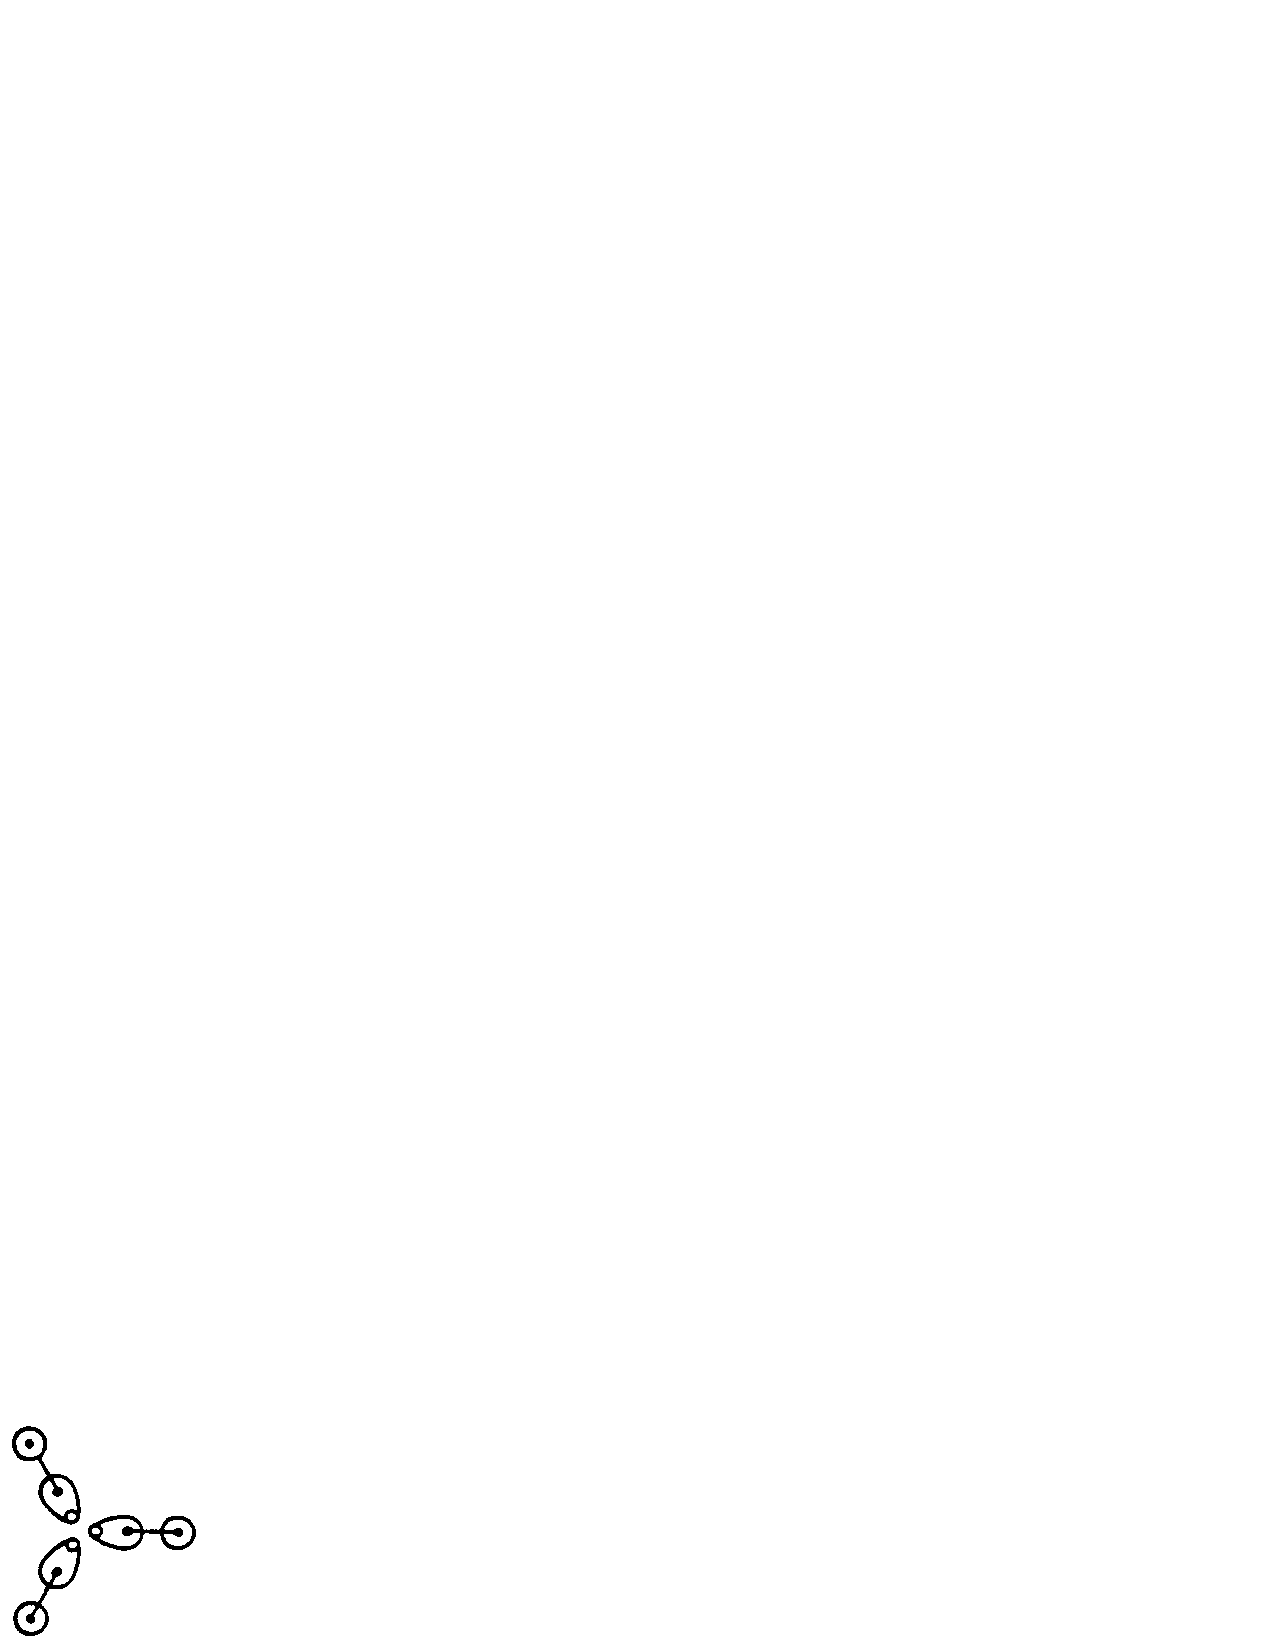
\includegraphics{fig6-06j}
\label{chap6-eqno24}
\end{equation}
As there are no additional valence orbitals available for bonding, a 
fourth H will not be bound to (\ref{chap6-eqno24}).  Again, van der Waals 
interactions can lead to a weak bond, $\leq$ 2 kcal, but we ignore 
such second-order effects here.

Considering, briefly, the relative bond energies of the series
$D_{Al-H}$, $D_{HAl-H}$, and $D_{H_2Al-H}$, the first and third bonds
involve unpaired Al orbitals, a $p$ orbital in the first and a lobe in
the third.  In order to make the second bond, however, it was
necessary to unpair the Al lobe orbitals, (\ref{chap6-eqno23}).  Thus,
the second bond energy will be at least 20 kcal smaller than either
the first or the third.

\subsection{Low-Lying States of PH$_n$}

Starting with the ground state of P, and bonding an H to any one of 
the three-singly-occupied $p$ orbitals, leads to the ${^3\Sigma}^-$ 
state of PH
\begin{equation}
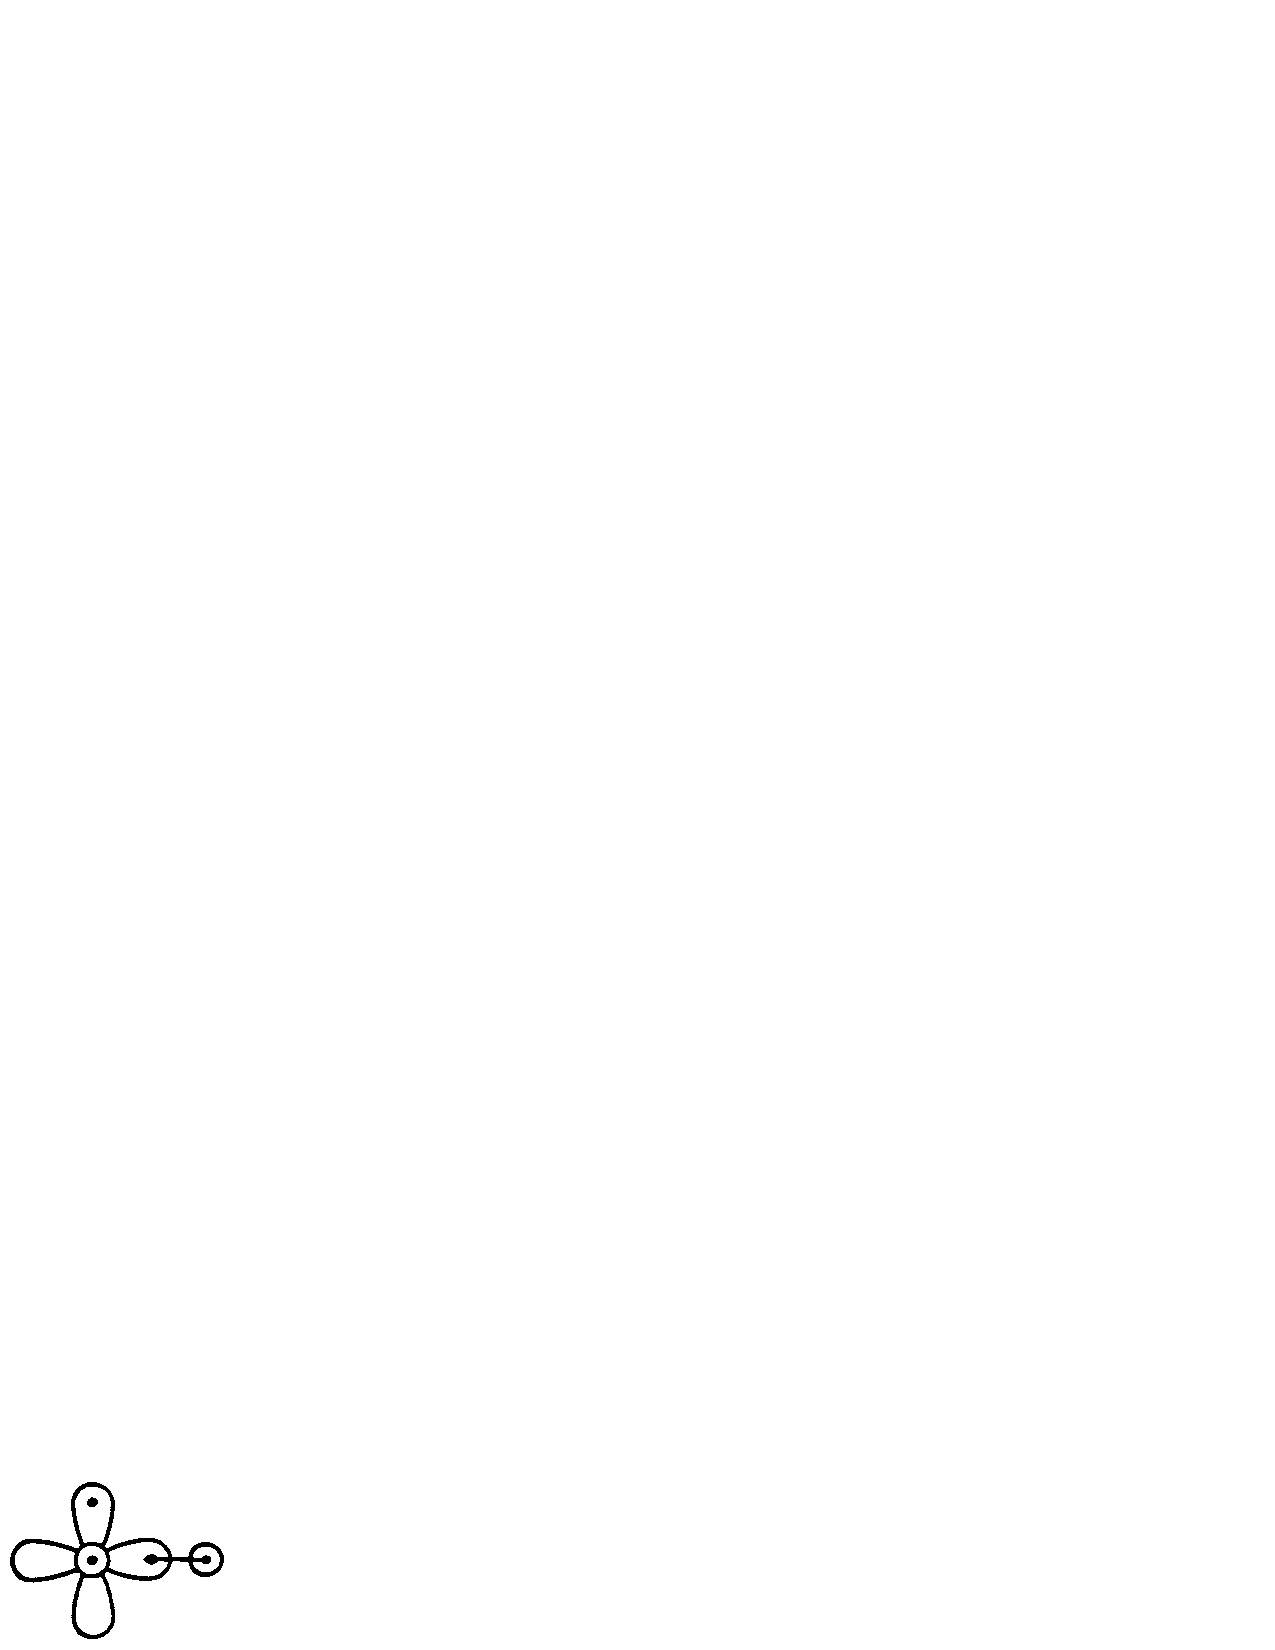
\includegraphics{fig6-06k}
\label{chap6-eqno25}
\end{equation}
Note that there is a doubly-occupied $3s$ pair, not shown in
(\ref{chap6-eqno25}).

Bonding an H to a second $p$ orbital, leads to the ${^2B}_1$ state of 
PH$_2$,
\begin{equation}
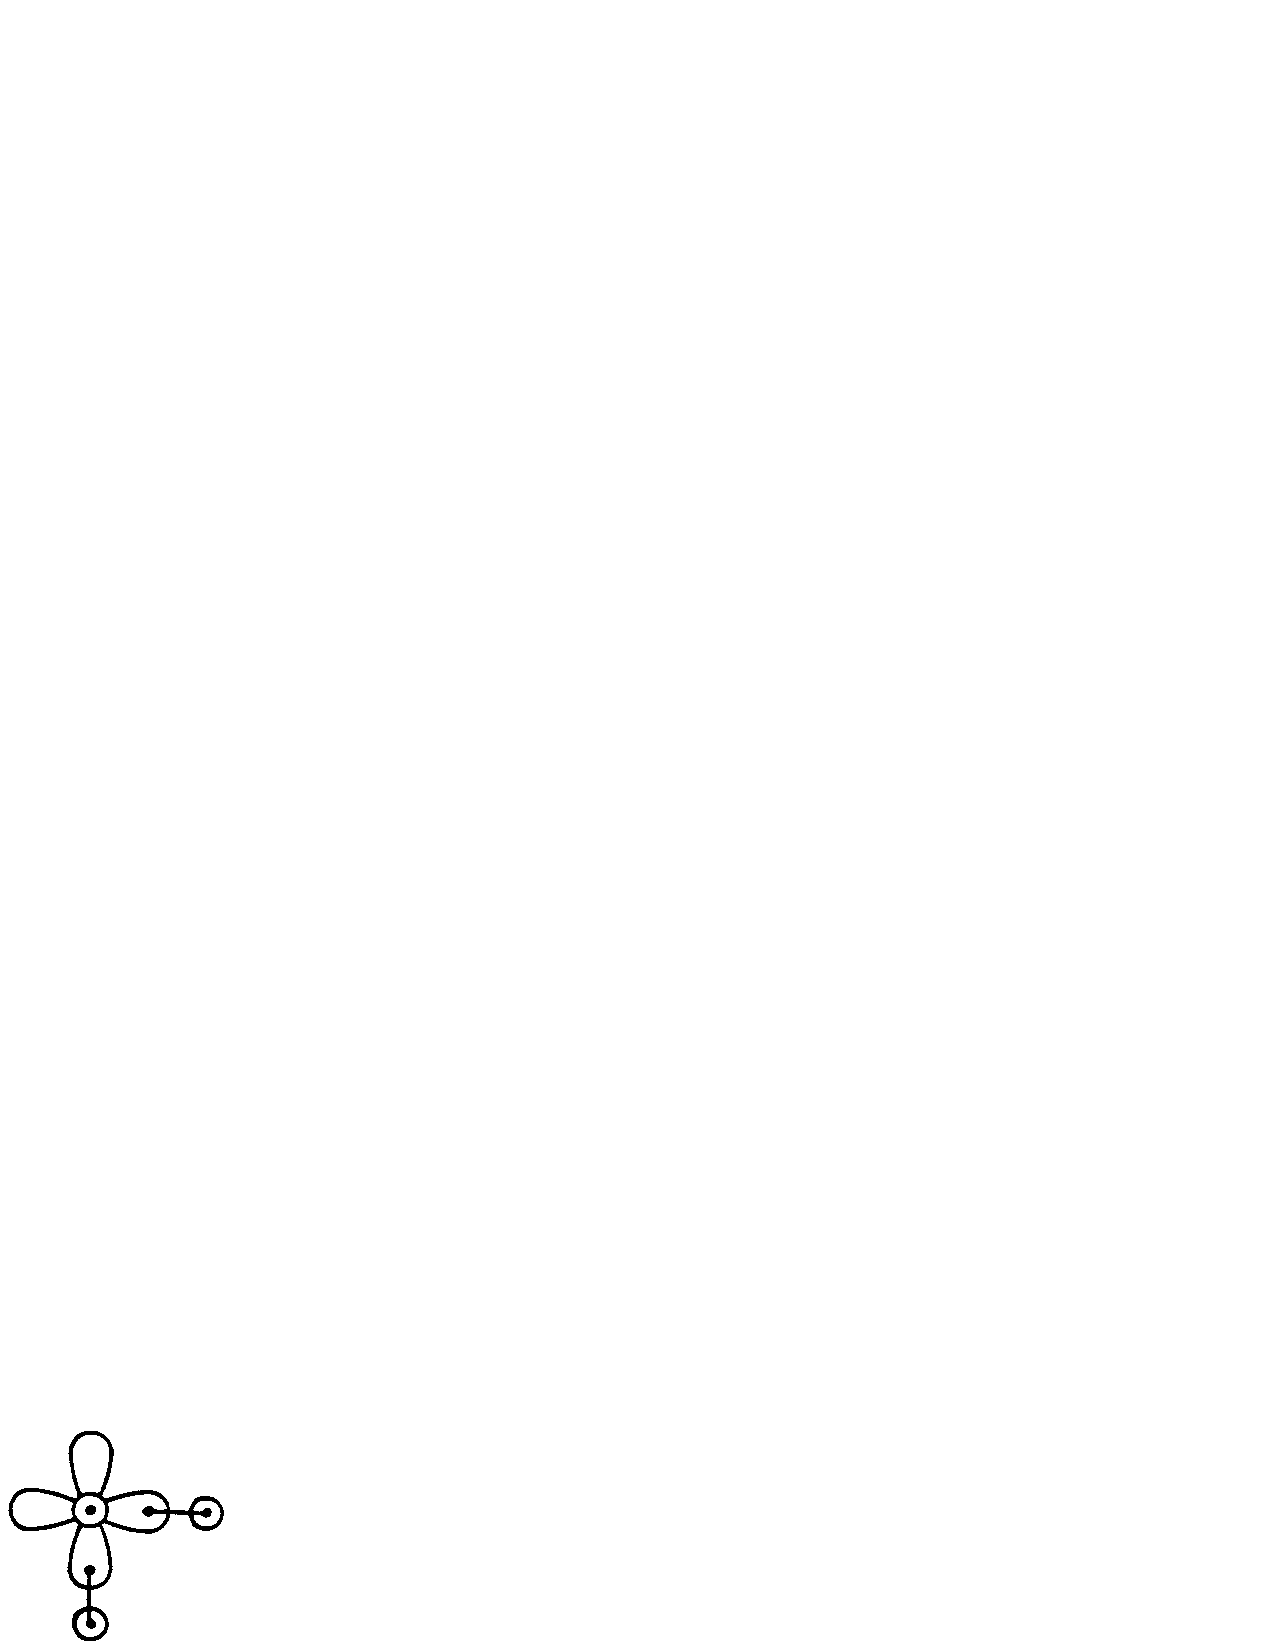
\includegraphics{fig6-06l}
\label{chap6-eqno26}
\end{equation}
Because the two bonds involve perpendicular $p$ orbitals, we would 
expect a bond angle of approximately 90$^{\circ}$.  In fact, the bond 
angle is slightly larger, 92$^{\circ}$, due to bond-bond repulsions, 
Pauli principle.  Bonding an H to the remaining singly-occupied $p$ 
orbital of PH$_2$, leads to the pyramidal ground state of PH$_3$.  
Again, the equilibrium bond angles are expected to be slightly larger 
than 90$^{\circ}$, the observed angles are 92.2$^{\circ}$.

All three bonds involve singly-occupied phosphorous $p$ orbitals, and 
hence, the three bond strengths should be comparable.  There will 
though, be a small, systematic change in the bond energies due to 
differences in the $p-p^{\prime}$ exchange interactions as discussed 
in a later section.  The result is that the bond strengths are in the 
order
\begin{equation}
D_\mathrm{P-H} < D_\mathrm{HP - H} < D_\mathrm{H_2P-H}.
\end{equation}

Bonding a fourth H to phosphorous requires the unpairing of the $3s$ 
pair.  The energy of this unpairing is larger than the bond energy, 
and hence, PH$_4$ should not be bound with respect to PH$_3$ plus H.

\subsection{Low-Lying States of SH$_n$}

Starting with the ground states of sulfur, and bonding an H to one of 
the two singly-occupied $p$ orbitals, leads to the ${^2\Pi}$ ground 
state of SH,
\begin{equation}
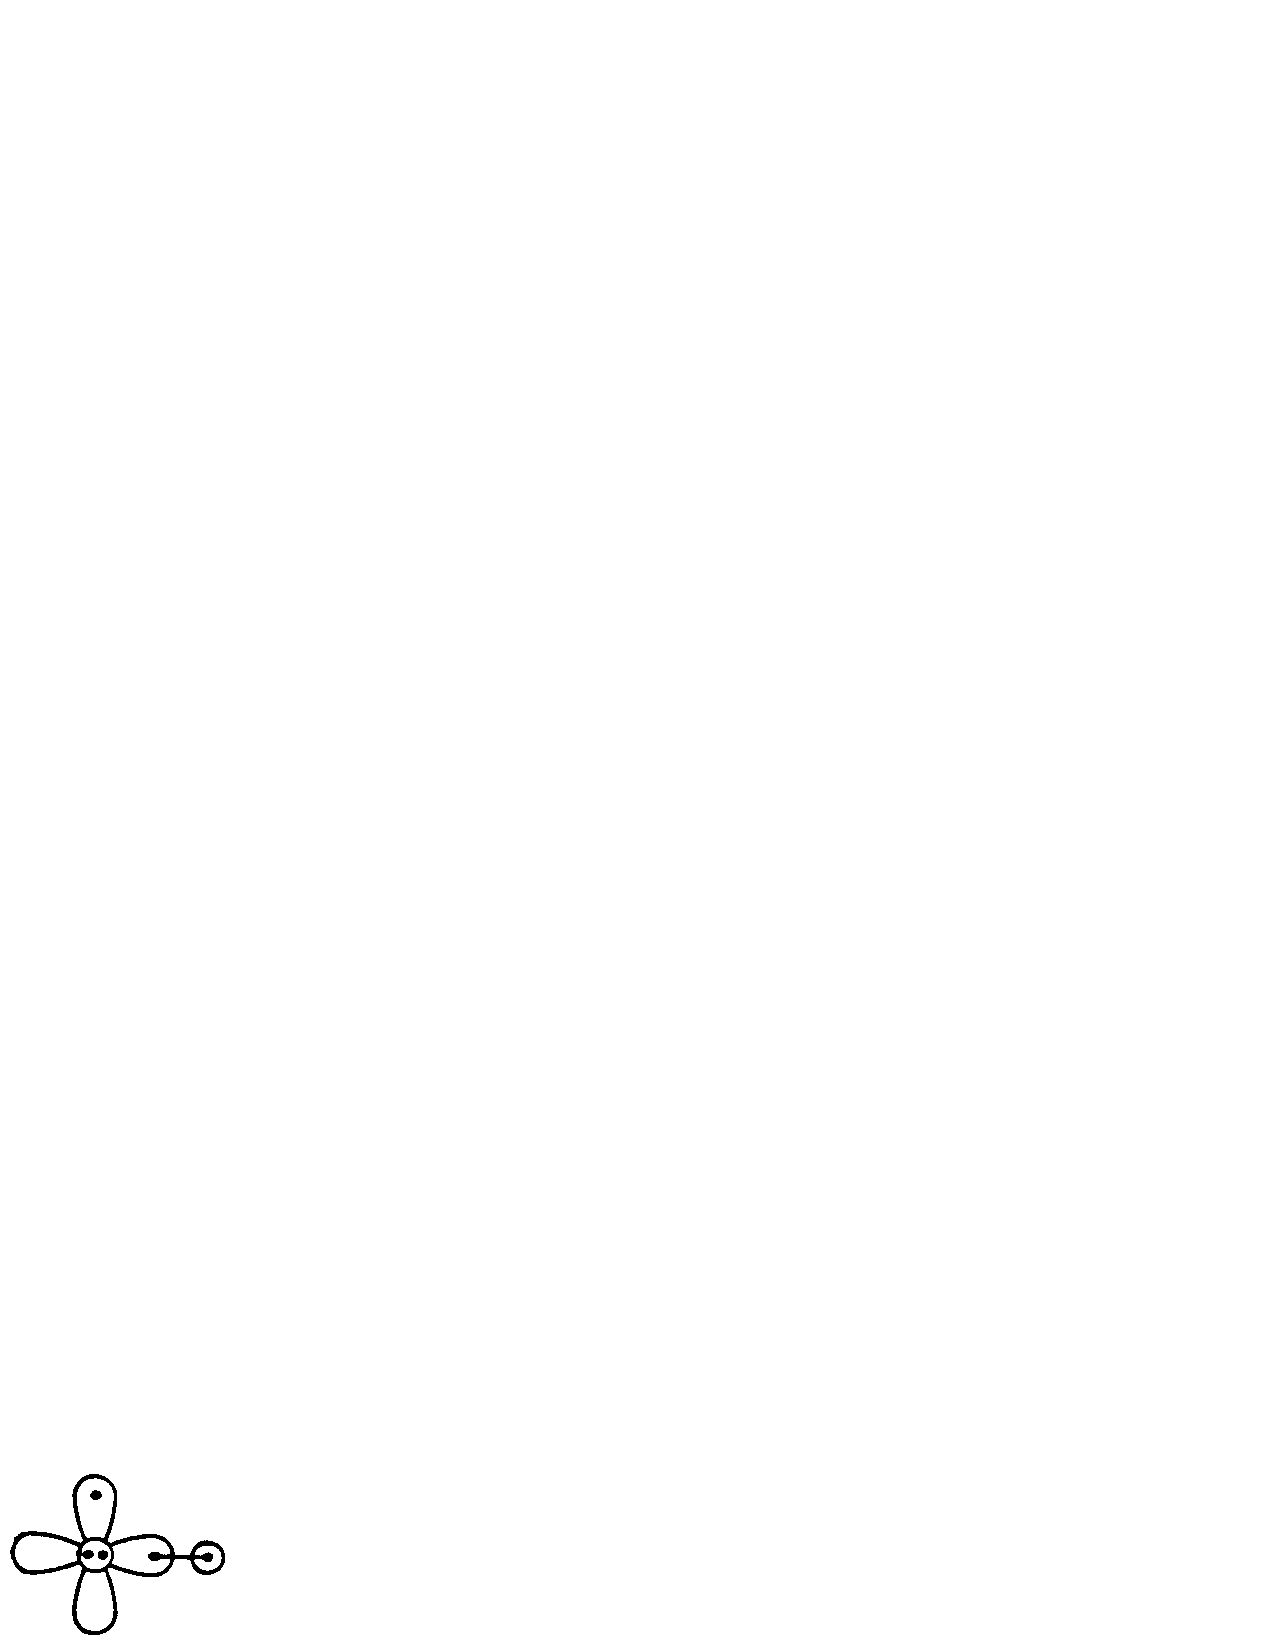
\includegraphics{fig6-06m}
\end{equation}
Bonding a second H, gives rise to the ${^1A}_1$ state of SH$_2$
\begin{equation}
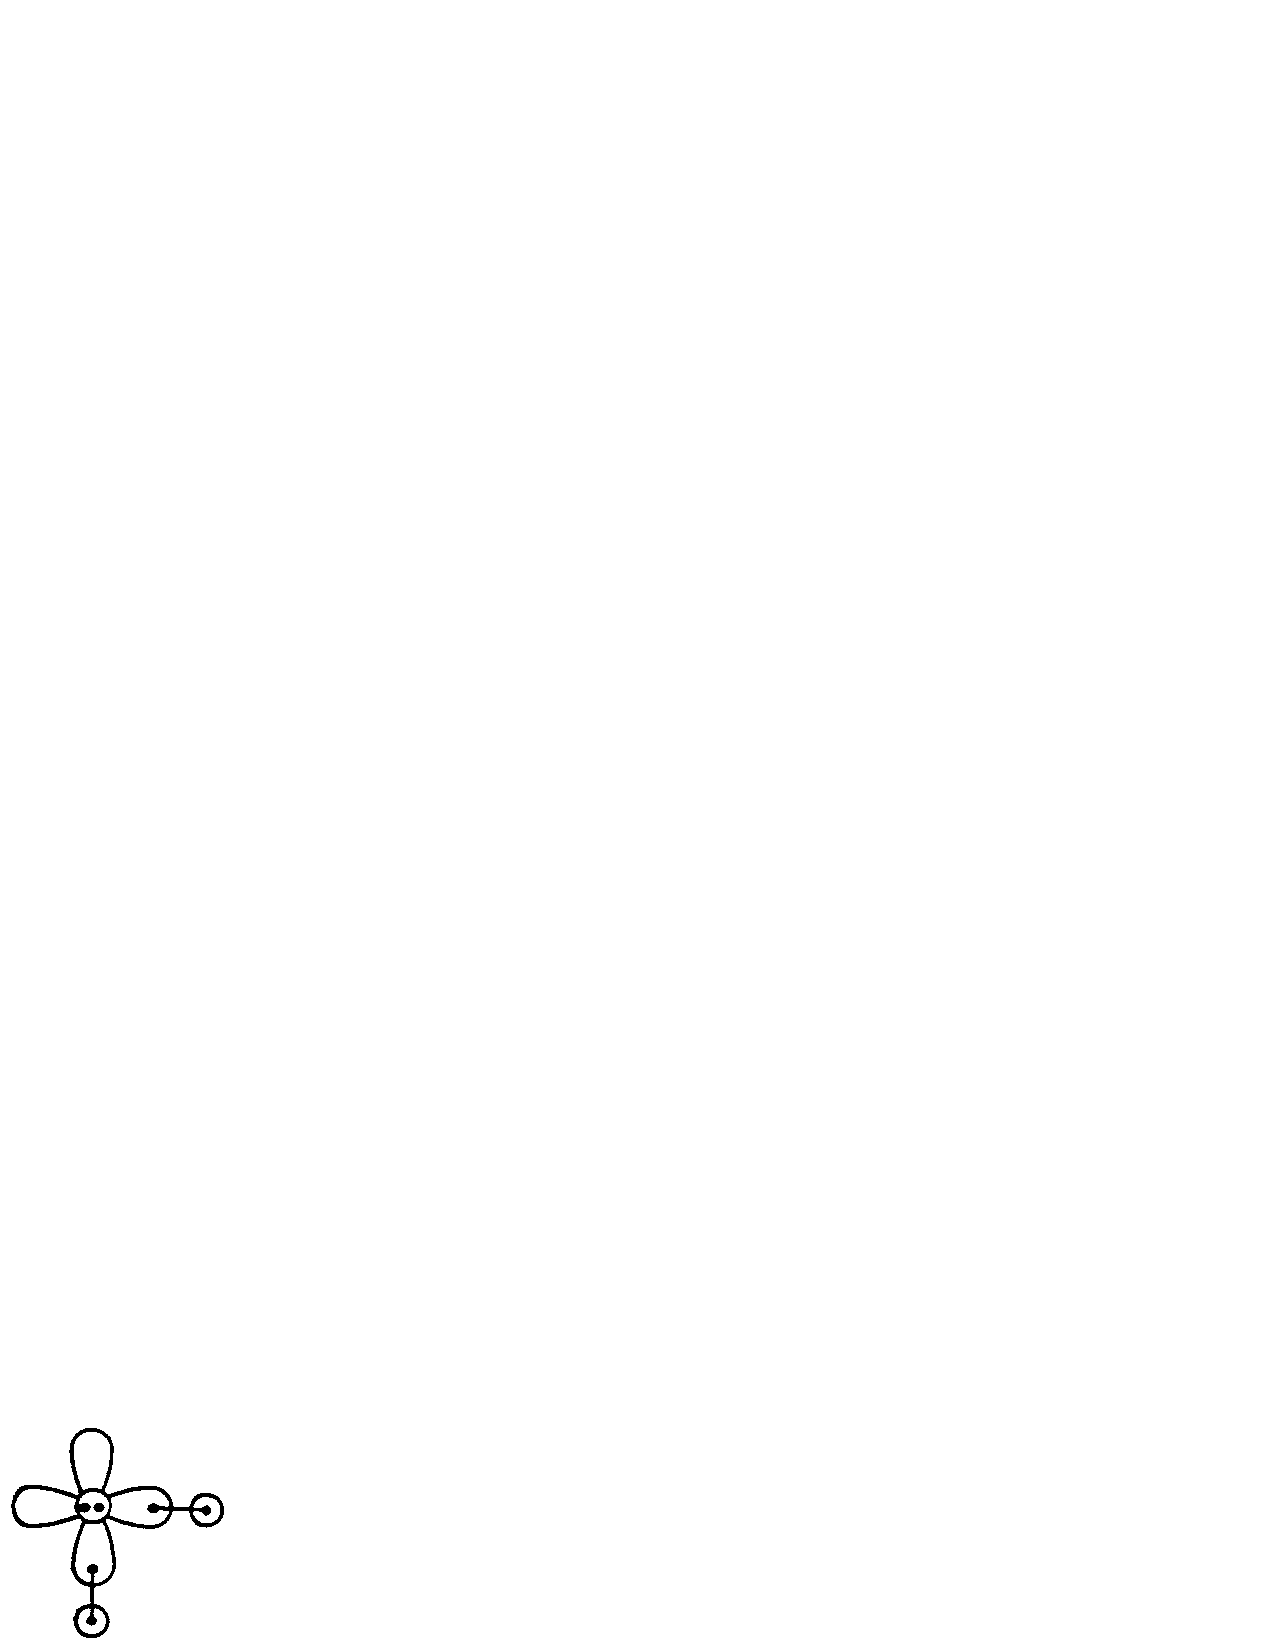
\includegraphics{fig6-06n}
\end{equation}
Because both bonds are two $p$ orbitals, the bond angle should be 
90$^{\circ}$.  However, bond-bond repulsions lead to the slightly 
larger angle of 92$^{\circ}$.

In order to bond a third H to sulfur, it is necessary to unpair the 
$3s$ electron pair.  Because the three $p$ orbitals of $s$ are 
occupied, the $3s$ pair of $s$ is not highly correlated, as it is in 
Mg, Al, and Si.  Thus, the energy required to uncouple the pair is 
larger than the resulting bond energy.  Hence, SH$_3$ should not be 
bound with respect to SH$_2$ plus H.

\subsection{The State of ClH$_n$ and ArH$_n$}

The ground state of Cl, includes one singly-occupied $p$ orbital.  
Bonding an H to this orbital, yields the ${^1\Sigma}^+$ ground state 
of HCl,
\begin{equation}
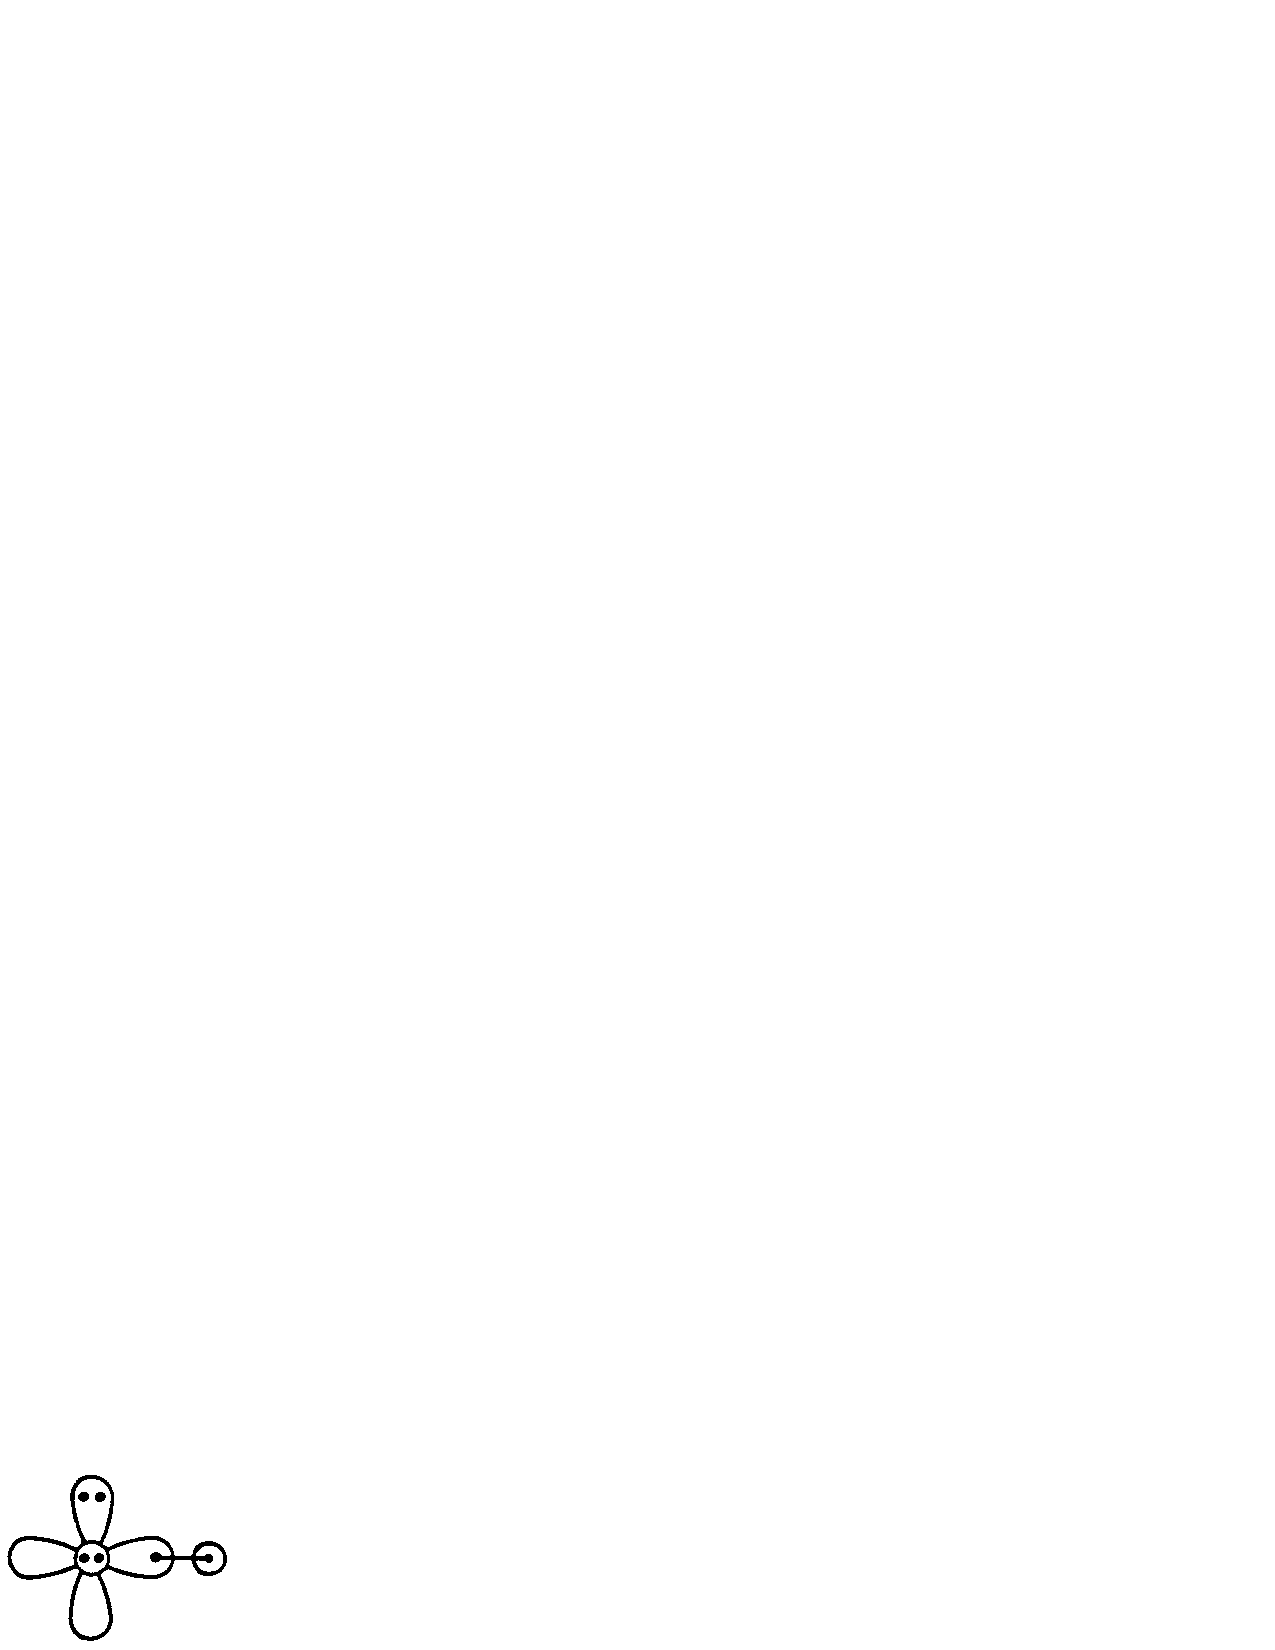
\includegraphics{fig6-06o}
\end{equation}
As there are no additional orbitals available for bonding, ClH$_2$ is 
not expected to be bound, nor are any low-lying bound excited states 
of ClH expected.  Starting with the configuraiton of Ar, we see that 
there is no favorable pairing with an H atom.

\section{First-Row Hydrides}

The principles of bonding, discussed in the previous sections, apply 
also to the hydrides of corresponding atoms of other rows of the 
periodic table.  For hydrides of non-transition metals atoms, below 
the second row, the qualitative description of bonding is identical to 
that of the second-row hydrides.  The presence of partially filled $d$ 
or $f$ shells can lead to more complicated effects.  For the first row 
hydrides, however, some of the qualitative aspects of bonding are 
different.  In this section, we will first discuss the origin of the 
differences, and then discuss the implications of these differences, 
taking the CH$_n$ and NH$_n$ series as examples.

\subsection{Bond-Bond Repulsions}

\begin{figure}
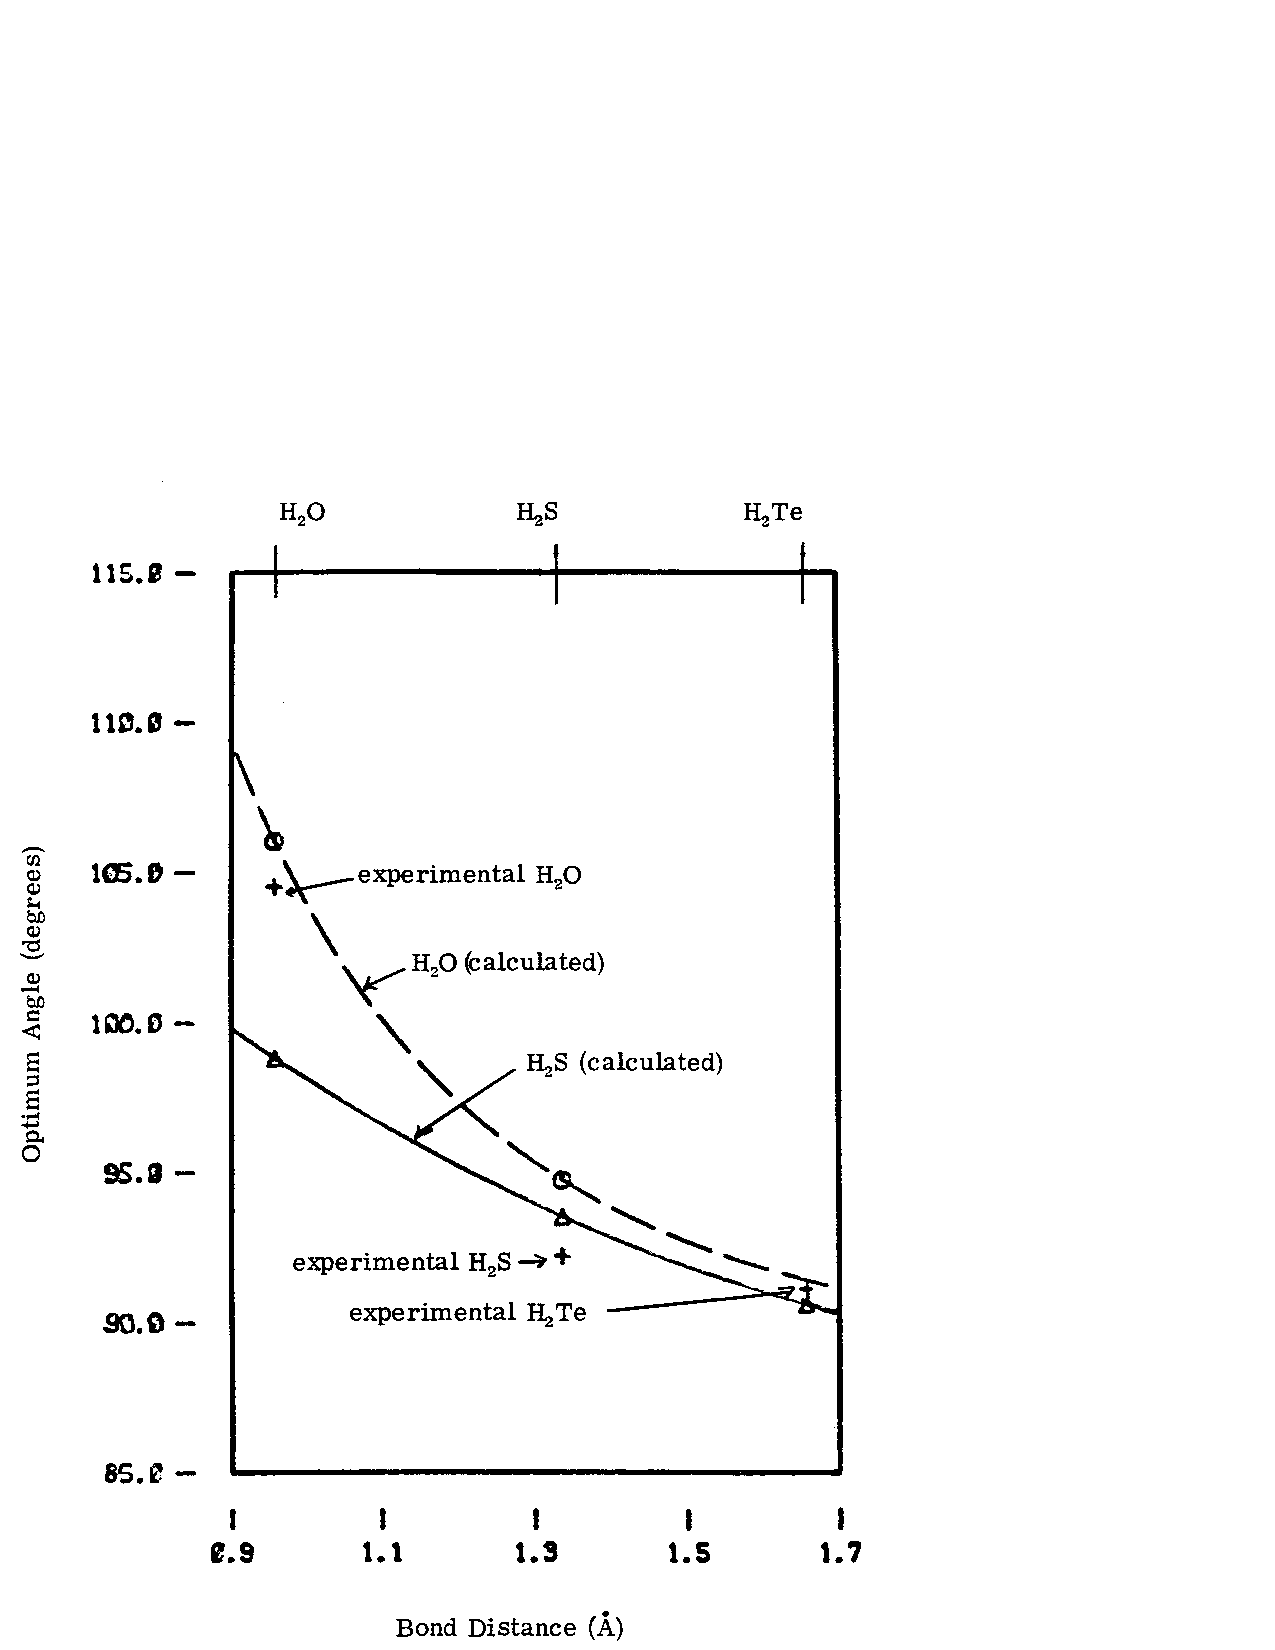
\includegraphics{fig6-06e}
\caption{Bond angles of H$_2$O and H$_2$S as a function 
of bond distance.  The calculation is valence bond zeta basis plus
diffuse functions plus optimized $d$ functions.$^{11}$ }
\label{chap6-fig7}
\end{figure}

In the simplest description, bonding two H atoms to two
singly-occupied $p$ orbitals would lead to a bond angle of
90$^{\circ}$.  For second-row atoms, Pauli principle repulsions
between the bond pairs increase these angles slightly to
91$^{\circ}$-93$^{\circ}$.  Assuming covalent bonds, this repulsive
interaction depends upon the overlap, squared, of the two H orbitals,
For SiH$_2$(${^1A}_1$), PH$_2$(${^2B}_1$), and SH$_2$(${^1A}_1$) the
H-H distances for two bonds at 90$^{\circ}$ are 2.148, 2.010, and
1.818 \AA.  However, for the corresponding first-row hydrides, CH$_2$,
NH$_2$, and OH$_2$, the bond lengths are approximately 30 percent
shorter, leading to H-H distances, for 90$^{\circ}$ bond angle, of
1.5712, 1.448, and 1.352 \AA.  This difference in H-H distances, leads
to an increase in the H-H overlap, for example, from 0.2532 for SH$_2$
to 0.445 for OH$_2$.  As a result, the optimum bond angles for the
first-row compounds are significantly larger, 102$^{\circ}$ for
CH$_2$(${^1A}_1$), NH$_+2$(${^2B}_1$), and 104$^{\circ}$ for
OH$_2$(${^1A}_1$), than those of their second-row counterparts.  Note
that for all three molecules, the simplest description of the bonding
involves two perpendicular $p$ orbitals, and hence, predicted bond
angles of 90$^{\circ}$, see Figure \ref{chap6-fig7}.

Recall for SiH(${^2\Pi}$), (\ref{chap6-eqno11}), the angle between the lobe orbitals 
and the bond is 128$^{\circ}$, corresponding to an angle between the 
two lobes of 104$^{\circ}$.  Thus, bonding an H to a lobe of 
SiH(${^2\Pi}$) and averaging the two bond pairs, would be expected to 
lead to an angle of 116$^{\circ}$ between the remaining lobe and each 
of the bonds.  In fact, the actual angle is somewhat larger, 
121$^{\circ}$, indicating that the dominant repulsive overlap is 
between the bond pairs and the lobe orbital, rather than between the 
two bond pairs.  Had the bond pair-bond pair repulsion been dominant, 
the readjustment would have been to increase the bond angle, thus 
decreasing the bond-lobe angles.

For CH(${^2\Pi}$), the bond-lobe angle is also 
128$^{\circ}$,$^{12,13}$ and thus, bonding an H to a lobe orbital of 
CH(${^2\Pi}$) would also be expected to lead to a bond-lobe angle 
of 116$^{\circ}$.  In this case, however, the actual angle is somewhat 
smaller, 113.5$^{\circ}$, indicating that for the frist-row compound 
the bond-bond repulsions are dominant.  Thus, the bond angle of 
CH$_2$(${^3B}_1$) is 113$^{\circ}$, 360-227, slightly larger than 
expected on the basis of the CH(${^2\Pi}$) bond-lobe angles.  
Similarly, the BH(${^1\Sigma}^+$), the bond-lobe angles are 
126$^{\circ}$,$^{14}$ while bonding a H to one of the lobes, leads to 
a bond angle of 131$^{\circ}$.  Thus, for CH$_2$ and BH$_2$, the bond 
angles are approximately 5$^{\circ}$ larger than the corresponding CH 
and BH bond-lobe angles.

In summary, for first-row hydrides, bond-bond repulsions lead to a 
12$^{\circ}$ to 15$^{\circ}$ increase in the bond angle between the 
$p$-like bonds, and to a 5$^{\circ}$ increase for the case involving 
one $p$-like and one lobe-like bond.  This effect is much larger for 
first row hydrides than for hydrides of any of the lower rows, simple 
because of the smaller bond lengths in the first-row hydrides.  A 
detailed comparison of bond lengths and bond angles, for first-row, 
second-row, and third-row hydrides is given in Table \ref{chap6-table1}.

\begin{table}
\caption{Summary of bond lengths and angles of the hydrides of the
first, second, and third rows of the periodic table.} 
\label{chap6-table1}

\begin{tabular}{cccccc}\\ \hline
GVB Diagram & State & Molecule &\multicolumn{2}{c} Bond Angle 
($\theta$) & Bond\cr
& & & Orbs. & Est. & Length (\AA)\cr

& ${^2\Sigma}^+$ & BeH & - & 180$^{\circ}$ & 1.343\cr
& & MgH & - & 180$^{\circ}$ & 1.730\cr

& ${^1\Sigma}^+$ & BeH$_2$ & - & 180$^{\circ}$\cr
& & MgH$_2$ & - & 180$^{\circ}$\cr
& & CaH$_2$ & - & 180$^{\circ}$\cr

& ${^1\Sigma}^+$ & BH & & 126$^{\circ}$ & 1.232\cr
& & AlH & & 128$^{\circ}$ & 1.648\cr
& & GaH & & (128$^{\circ}$) & 1.663\cr

& ${^2A}_1$ & BH$_2$ & 131$^{\circ}$ & 126$^{\circ}$ & 1.181\cr
& & AlH$_3$ & 119$^{\circ}$ & 128$^{\circ}$ & 1.59\cr
& & GaH$_2$ & & 128$^{\circ}$\cr

& ${^1A}^{\prime}$ & BH$_3$ & 120$^{\circ}$ &120$^{\circ}$\cr
& & AlH$_3$ & 120$^{\circ}$ &120$^{\circ}$\cr
& & GaH$_3$ & 120$^{\circ}$ &120$^{\circ}$\cr

& ${^2\Pi}$ & CH & - & 128$^{\circ}$  & 1.120\cr
& & SiH & - & 128$^{\circ}$ & 1.516\cr
& & GeH & - & (128$^{\circ}$) & 1.588\cr

& ${^1A}_1$ & CH$_2$ & 102.4 & 90$^{\circ}$ & 1.113\cr
& & SiH$_2$ & 92.1 &  90$^{\circ}$ & 1.516\cr
& & GeH$_2$ & (91$^{\circ}$) & 90$^{\circ}$\cr

& ${^3B}_1$ & CH$_2$ & 133.2$^{\circ}$ & 128$^{\circ}$ & 1.084\cr
& & SiH$_2$ & 117.8$^{\circ}$ & 128$^{\circ}$ & 1.485\cr
& & GeH$_2$ & & (128$^{\circ}$)\cr

& ${^2A}^{\prime}$ & CH$_3$ & 120$^{\circ}$ & 120$^{\circ}$\cr

& ${^2A}$ & ~~ GeH$_3$ ~~\cr
& & CH$_4$\cr
& & SiH$_4$ & & & 1.479\cr
& & GeH$_4$\cr

& ${^3\Sigma}^-$ & NH & - & & 1.035\cr
& & PH & - & & (1.433)\cr
& & AsH & - & & 1.534\cr

& ${^3B}_1$ & NH$_2$ & 103.3$^{\circ}$ & 90$^{\circ}$ & 1.024\cr
& & PH$_2$ & 91.7$^{\circ}$ & ~~ 90$^{\circ}$ ~~ & ~~ 1.418\cr
& & AsH$_2$ & 90.7$^{\circ}$ & & 1.518\cr

& ${^2A}_1$ & NH$_2$ & 143.3$^{\circ}$ & & 1.000\cr
& & PH$_2$ & 123.1$^{\circ}$ & & 1.403\cr
& & AsH$_2$\cr

& ${^1A}$ & NH$_3$ & 106.7$^{\circ}$ & 90$^{\circ}$ & 1.012\cr
& & PH$_3$ & 93.3$^{\circ}$ & 90$^{\circ}$ & 1.420\cr
& & AsH$_3$ & 92.1$^{\circ}$ & 90$^{\circ}$ & 1.511\cr

& ${^2\Pi}$ & OH & - & & 0.970\cr
& & SH & - & & 1.341\cr
& & SeH & - & & (1.475)\cr

& ${^1A}_1$ & OH$_2$ & 104.5$^{\circ}$ & 90$^{\circ}$ & 0.958\cr
& & SH$_2$ & 92.1$^{\circ}$ & 90$^{\circ}$ & 1.336\cr
& & SeH$_2$ & 90.6$^{\circ}$ & 90$^{\circ}$ & 1.460\cr
& & TeH$_2$ & 90.2$^{\circ}$ & & 1.658\cr

& ${^1\Sigma}^+_g$ & FH & - & - & 0.917\cr
& & ClH & - & - & 1.275\cr
& & BrH & - & - & 1.414\cr
& & IH & & & 1.609\cr 
\hline
\end{tabular}
\end{table}

\subsection{Relative Strengths of Bonds}

A second factor, distinguishing the first-row atoms from the others, 
is that the sizes of the $s$ and $p$ orbitals are comparable for the 
first row.  Whereas for lower rows, the $s$ orbitals are significantly 
smaller than the $p$ orbitals.  The comparison of sizes is shown in 
Chapter 5, where the valence $s$ and $p$ orbitals are compared for 
the first four fows of the periodic table.

The origin of this difference is, considering the first-row atoms, the 
valence $2s$ orbital penetrates the $1s$ core more effectively than 
does the $2p$ orbital.  Balancing this effect, however, is the 
constraint that the $2s$ orbital must remain orthogonal to the $1s$ 
orbital.  No such constraint exists for the $2p$ orbitals.  For atoms 
from the lower rows, the valence $s$ orbitals still penetrate the 
core more effectively than do the valence $p$ orbitals.  However, in 
these atoms, both the valence $s$ and the valence $p$ orbitals are 
subject to orthogonality constraints, involving core orbitals.  The 
result is, that for atoms of the second row, and below, the valence 
$s$ orbital is significantly more contracted than the valence $p$ 
orbitals.  Whereas for first-row atoms, the penetration and 
orthogonality effects nearly cancel.  Thus, there is a smaller 
difference between the valence $s$ and $p$ sizes of the first row 
than for any of the lower rows.  This similarity in size, of the first 
row $2s$ and $2p$ orbitals, leads to an increased importance of 
$2s-2p$ correlation, and thus, a decreased overlap between the low 
lobe orbitals.  For example, for Al, the overlap between the $\ell$ 
and ${\bar{\ell}}$ lobes is$^{15}$ 0.74.  Whereas, for B, this overlap 
is$^{14}$ 0.68.  Thus, for first row compounds, bonds to lobe orbitals 
are significantly more favorable, relative to $p$ bonds, than for 
other rows.

\subsection{Low-Lying States of CH$_n$}

The lowest states of CH arise from bonding an H to either a carbon 
$p$ orbital, forming the ${^2\Pi}$ ground state,
\begin{equation}
% missing figure (#55 in notes)
\end{equation}
or to a lobe orbital forming the ${^4\Sigma}^-$ state,
\begin{equation}
% missing figure (#56 in notes)
\end{equation}
The order of these states is identical to that found for SiH.  
However, the corresponding excitation energies differ considerably in 
magnitude.  For example, the lowest (${^4\Sigma}^-$) of the 
lobe-bonded states of CH lies$^{16}$ 17 kcal above the ground, 
$p$-bonded, state.  This is less than half the corresponding 
excitation energy of SiH, as expected from the above analysis.

Starting with the ${^2\Pi}$ state of CH, the lowest states of CH$_2$ 
are obtained by bonding an H, either to a $p$ orbital leading to the 
${^1A}_1$ state,
\begin{equation}
% missing figure (#57 in notes)
\end{equation}
or a lobe orbital (${^3B}_1$) state,
\begin{equation}
% missing figure (#58 in notes)
\label{chap6-eqno27}
\end{equation}
For SiH$_2$, the ground state (\ref{chap6-eqno15}) is ${^1A}_1$ with
the ${^3B}_1$ state (\ref{chap6-eqno14}) lying 18 kcal higher.
Comparing CH$_2$ with SiH$_2$, there are two important factors in
CH$_2$ favoring the ${^3B}_1$ state relative to the ${^1A}_1$.  First,
the bonds of the ${^1A}_1$ state involve perpendicular $p$ orbitals,
and hence, will favor small bond angles, approximately 90$^{\circ}$.
The bonds in the ${^3B}_1$ state, favor larger angles, approximately
128$^{\circ}$, {\it vide supra}. For first row compounds, the
importance of bond-bond repulsions, which are, of course largest at
small bond angles, leads to a significant increase in the energies of
states involving small bond angles, relative to those with larger
angles.  This effects increases the energy of the ${^1A}_1$ state
relative to the ${^3B}_1$ state.  The second factor, for first row
atoms lobe orbital, are more comparable, energetically, to $p$ orbital
bonds than for the Si row.  The ${^1A}_1$ state involves two bonds to
$p$ orbitals, while the ${^3B}_1$ state involves one $p$ bond and one
lobe bond.  Thus, this effect also lowers the energy of the ${^3B}_1$
state relative to the ${^1A}_1$ state for CH$_2$.

\begin{figure}
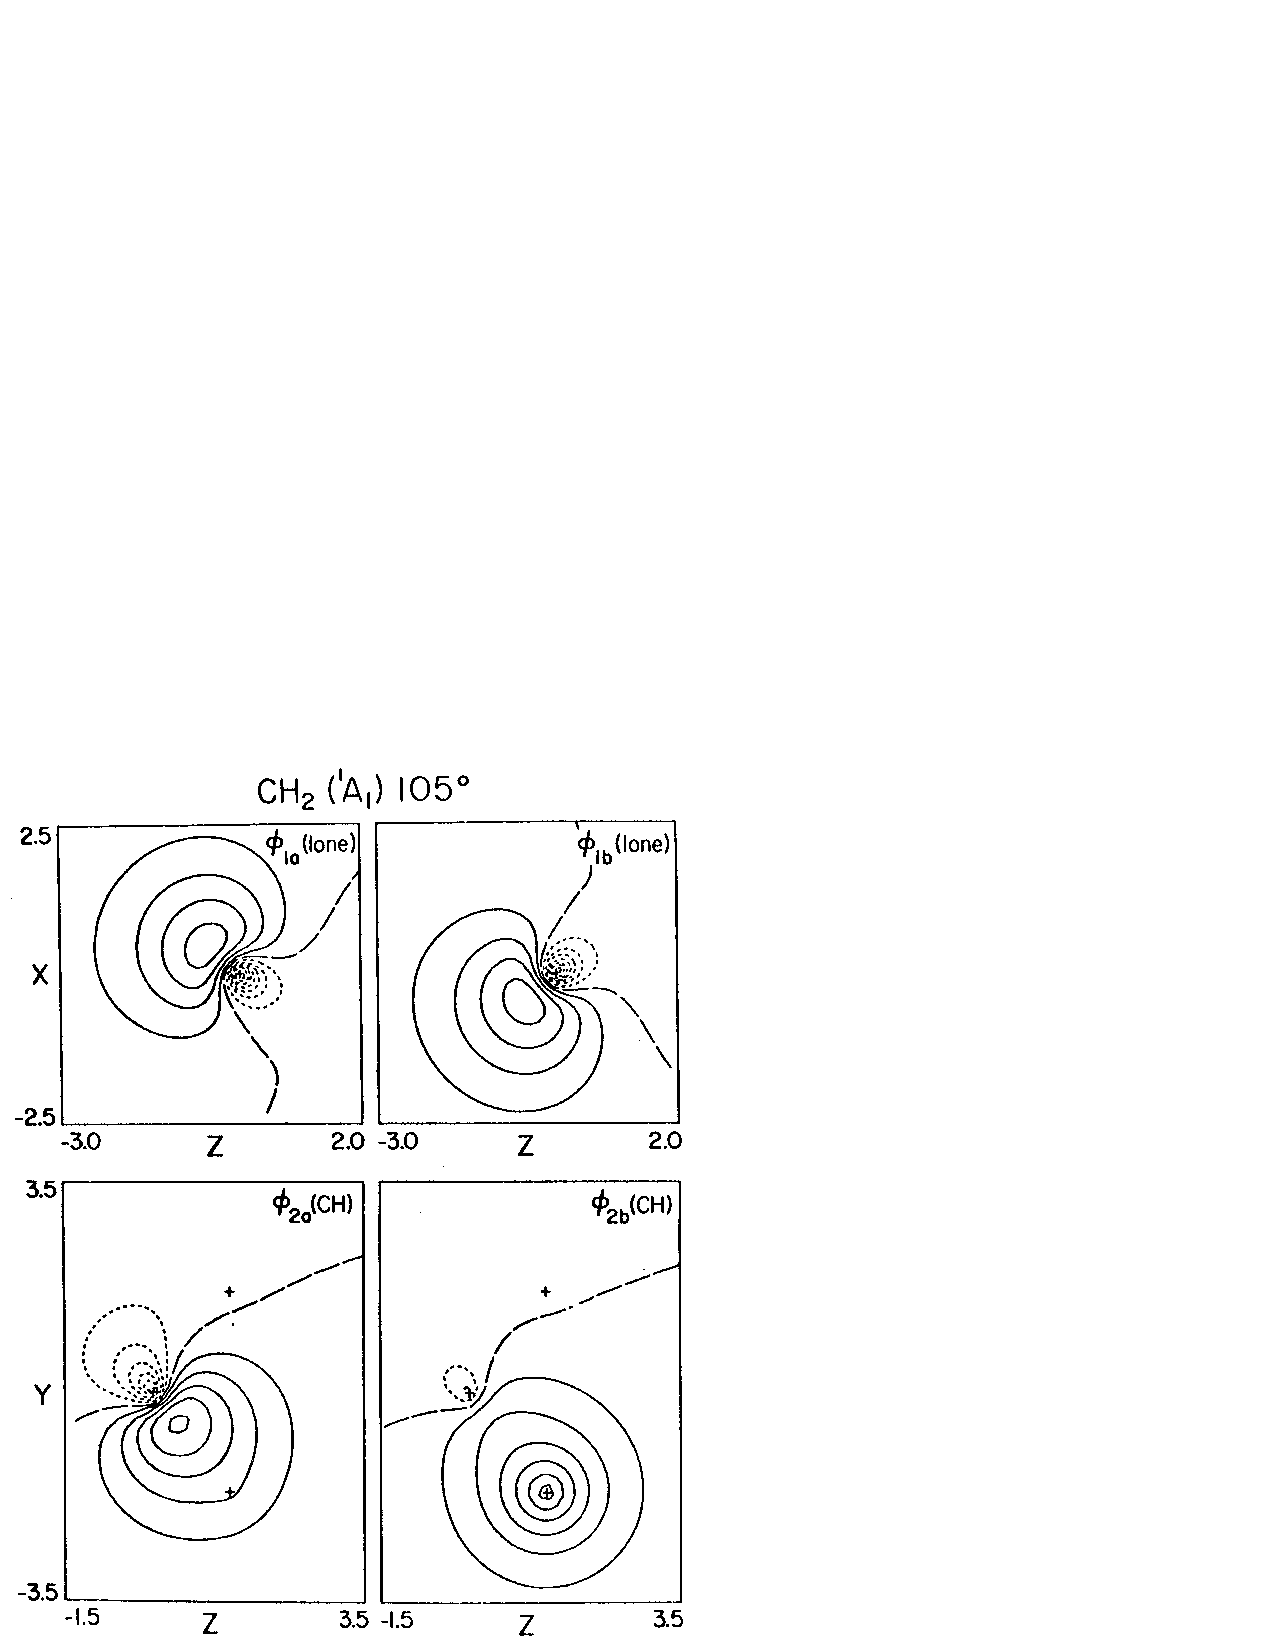
\includegraphics{fig6-07}
\caption{GVB orbitals of the ${^1A}_1$ state of CH$_2$, 
$\theta = 105^{\circ}$.$^{12}$ }
\label{chap6-fig8}
\end{figure}

\begin{figure}
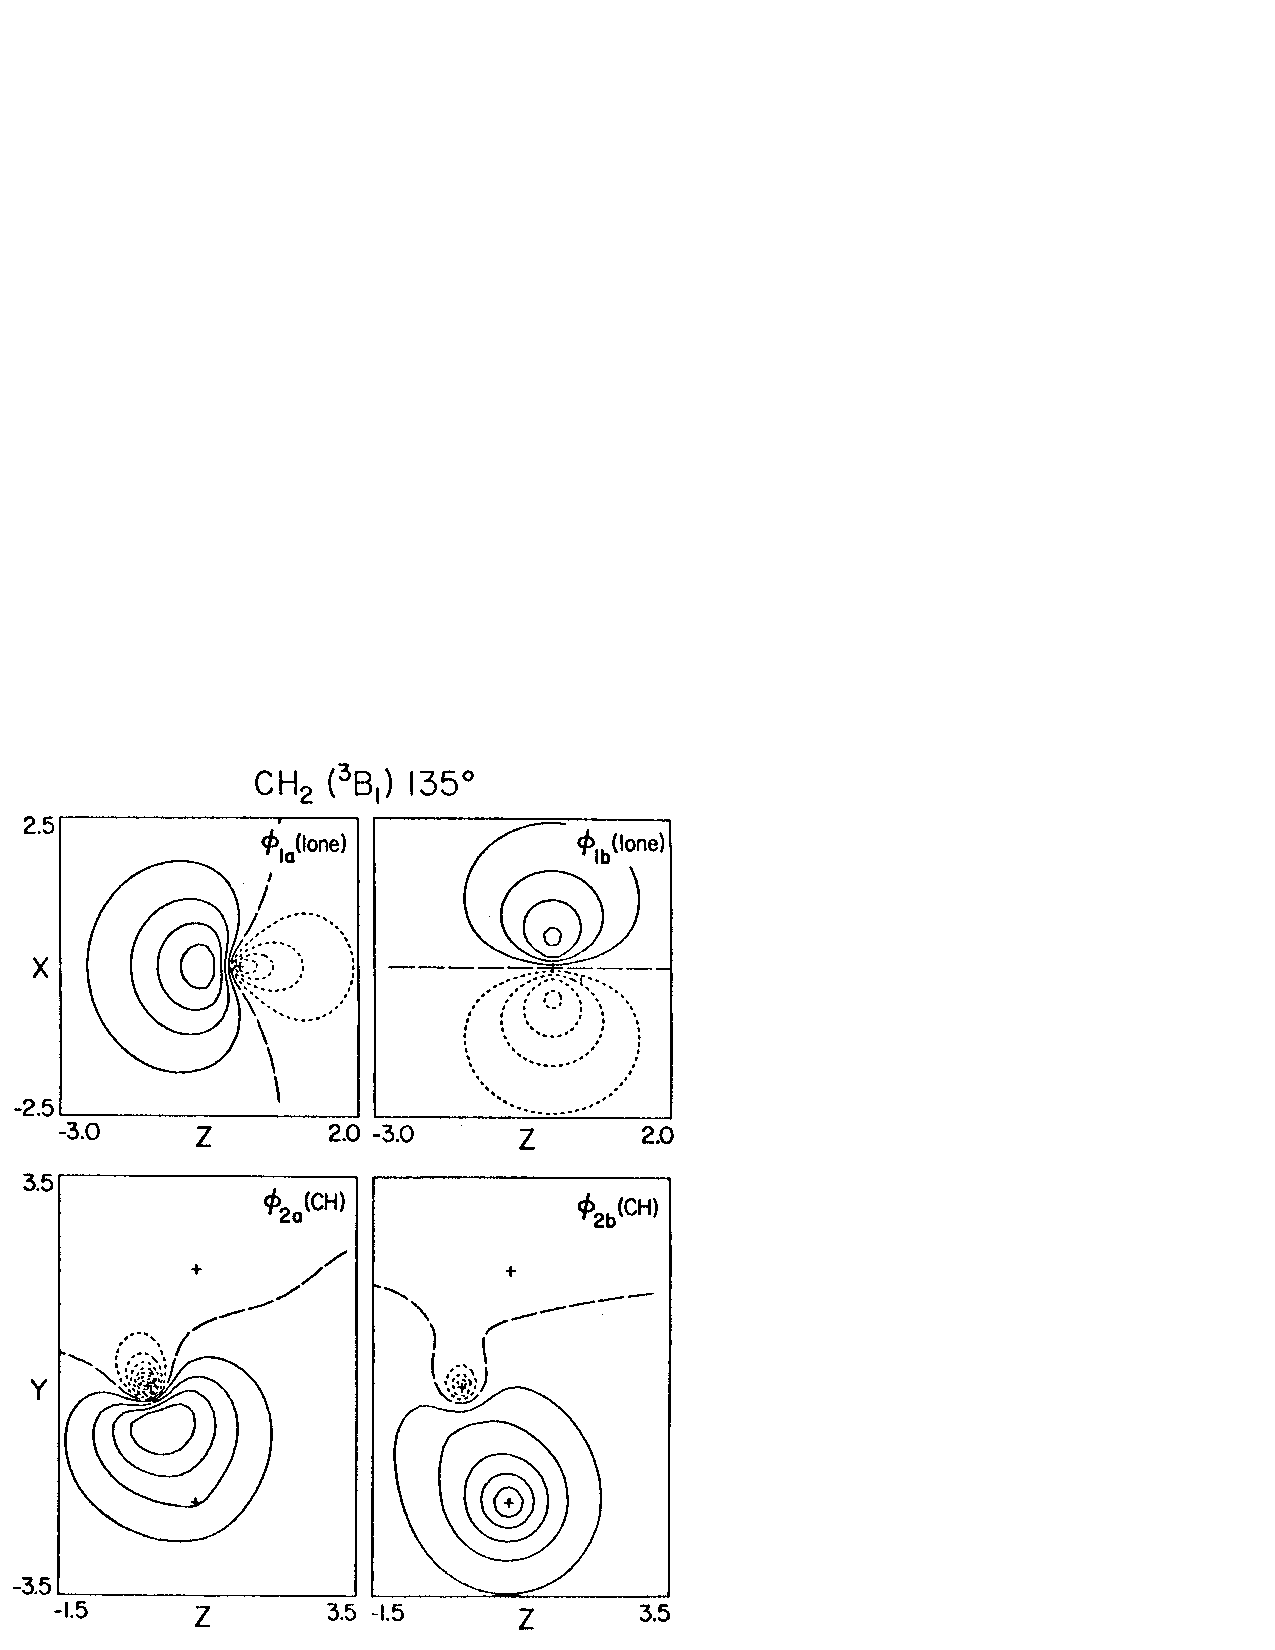
\includegraphics{fig6-08}
\caption{GVB orbitals of the ${^3B}_1$ state of CH$_2$,
$\theta = 135^{\circ}$.$^{12}$}
\label{chap6-fig9}
\end{figure}

The net result is that the ordering of the first two states of CH$_2$
is inverted with respect to SiH$_2$.  Thus, the ground state of CH$_2$
is the ${^3B}_1$ state which lies 9 kcal$^{16,17}$ below the ${^1A}_1$
state.  While for SiH$_2$, the ${^3B}_1$ state is 18 kcal above$^{11}$
${^1A}_1$.  The optimum orbitals for CH$_2$ are shown in Figures 
\ref{chap6-fig8} and \ref{chap6-fig9}, compare with Figures 
\ref{chap6-fig4} and \ref{chap6-fig5} for SiH$_2$.  

Starting with the ${^3B}_1$ ground state of CH$_2$,
(\ref{chap6-eqno26}), there are two possibilities for bonding a third
hydrogen, the unpaired lobe orbital (\ref{chap6-eqno28}, left), or the
$p \pi$ orbital (\ref{chap6-eqno28}, right),
\begin{equation}
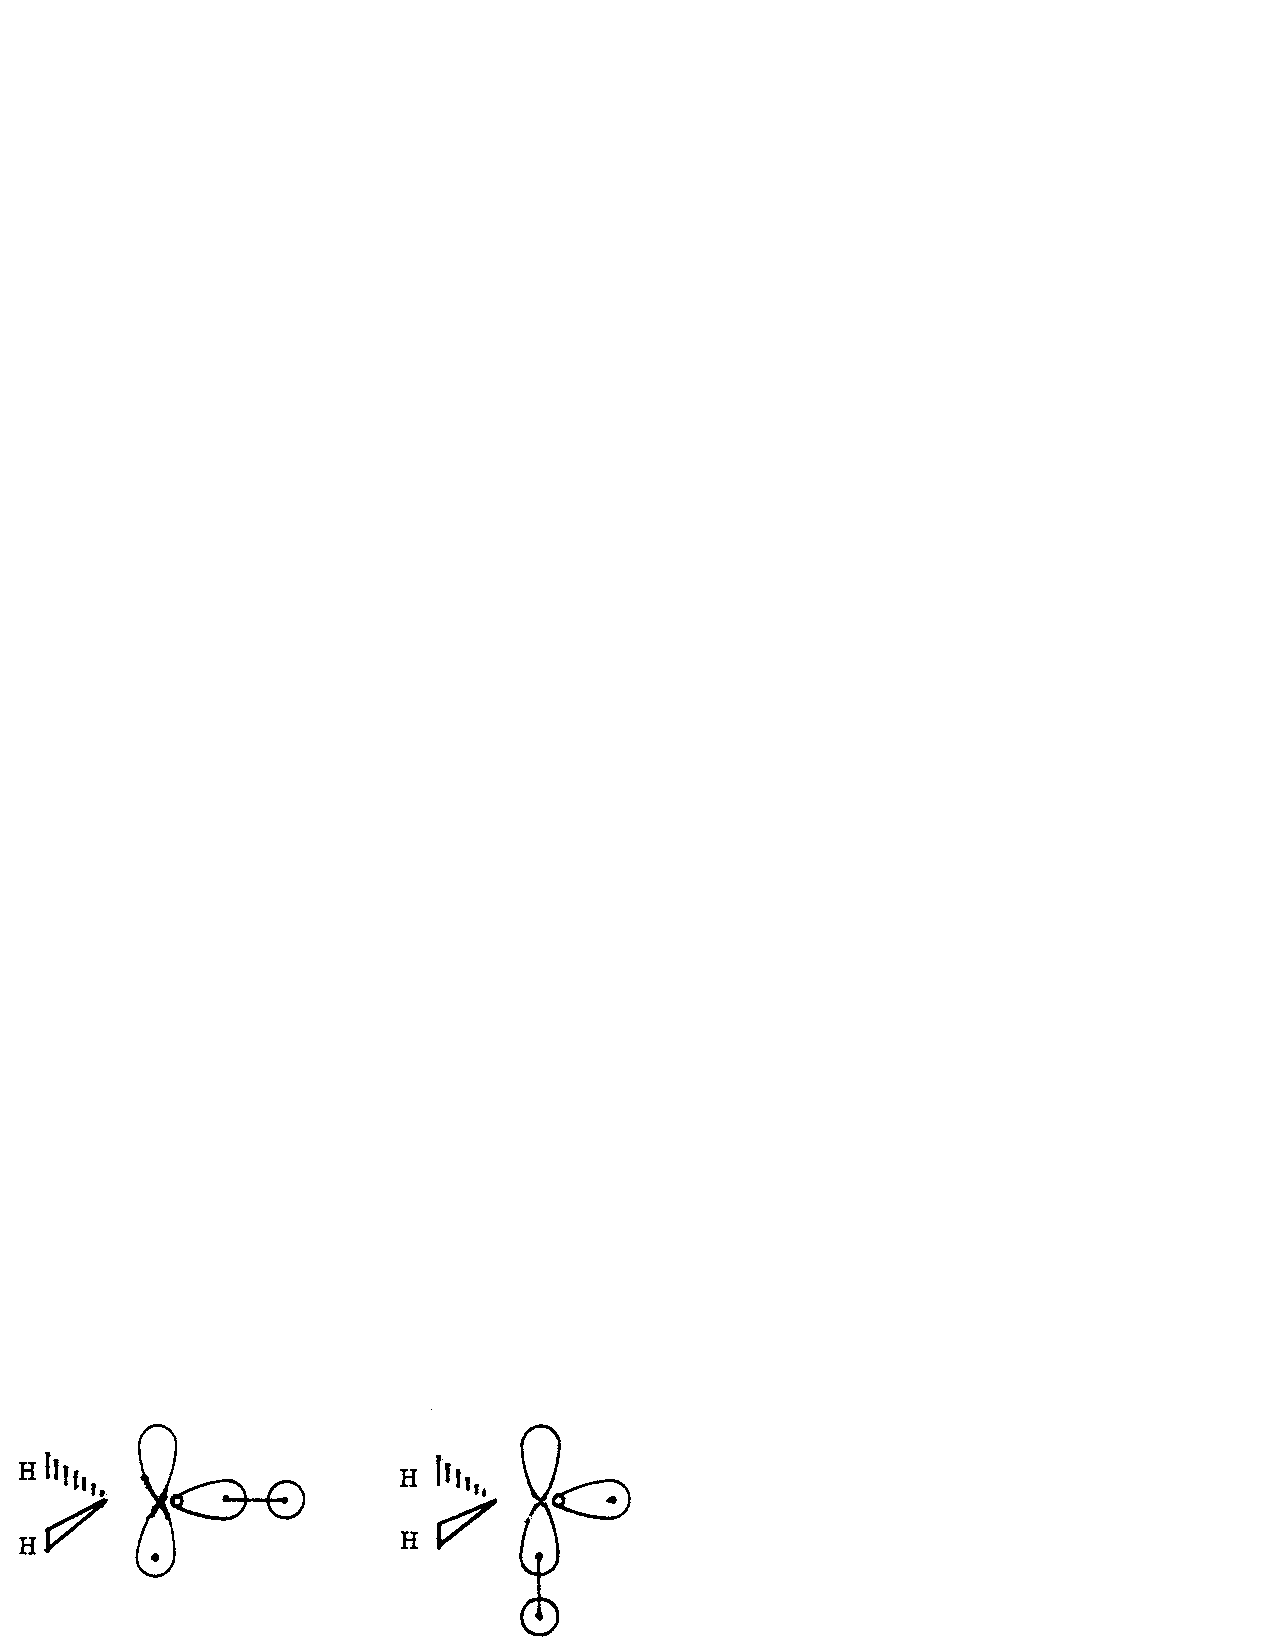
\includegraphics{fig6-08a}
\label{chap6-eqno28}
\end{equation}
Again, due to the importance of bond-bond interactions, the lower
configuration will be the one with the larger bond angles.  Bonding to
the lobe (\ref{chap6-eqno28}, left) leads to planar CH$_3$,
120$^{\circ}$ bond angles, while bonding to the $p \pi$ orbital
(\ref{chap6-eqno28}, right), leads to two 90$^{\circ}$ bond angles.
Thus, the lowest energy configuration of CH$_3$ is planar, whereas
SiH$_3$ was found to be pyramidal.  Because of the ability of
${^3B}_1$ CH$_2$ to bond an H to either the lobe or $p$ orbital, the
first constant for pyramidal distortion of CH$_3$ is quite
small.$^{18}$ The optimum orbitals for CH$_3$ and CH$_4$ are shown in
Figure \ref{chap6-fig10}.


\begin{figure}
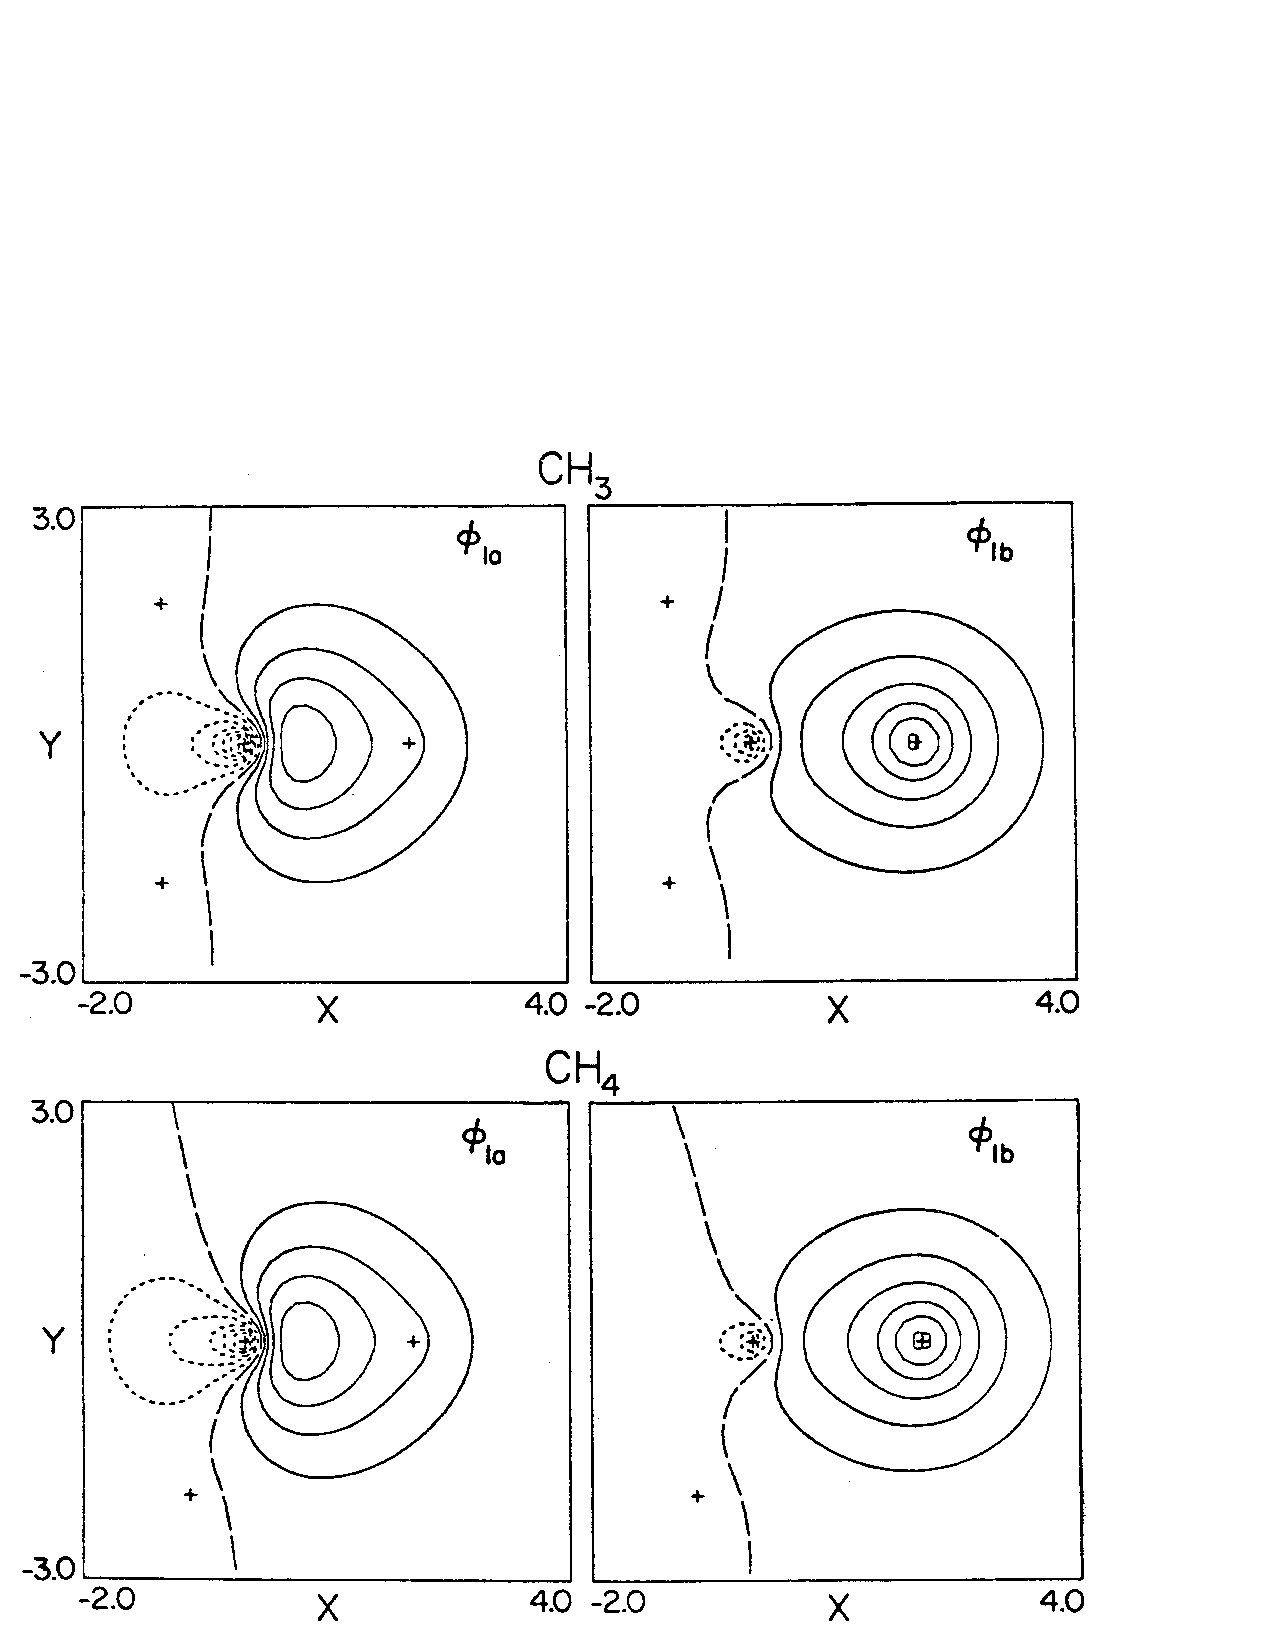
\includegraphics[scale=0.75]{fig6-09}
\caption{GVB orbitals for CH$_3$ and CH$_4$.}
\label{chap6-fig10}
\end{figure}

\subsection{Hybridization}

The tetravalency of C has long been known.  After quantum mechanics, 
and the Aufbau model of the atom, it was realized that C has a 
$(1s)^2(2s)^2(2p)^2$ configuration.  It was presumed that closed 
shells could not participate in bonding, and hence, this state of C 
would lead to divalency.  It was noticed, however, that the ${^5S}$ 
state, with configuration
\begin{equation}
(1s)^2(2s)^1(2p)^3
\label{chap6-eqno30}
\end{equation}
was only 3 eV above the ground state.  This state has four unpaired
orbitals, and hence, should be able to participate in four bonds,
tetravalency.  However, the four orbitals of (\ref{chap6-eqno30}) are
not equivalent.

Pauling suggested that the orbitals of (\ref{chap6-eqno30}) be
recombined, hybridized, so as to lead to four equivalent orbitals
pointing at the vertices of a tetrahedron centered at the C.  The
combinations of orbitals that do this are
\begin{eqnarray}
&{1 \over 2} \left( s + px + py + pz \right)& \cr
&{1 \over 2} \left( s - px - py + pz \right)& \cr
&{1 \over 2} \left( s - px + py - pz \right)& \cr
&{1 \over 2} \left( s + px - py - pz \right)& 
\end{eqnarray}
which are called $sp^3$ hybrides (75 \% $p$ character).

In some cases, trivalent bonding is observed.  In such cases, it was 
suggested that the appropriate hybrides are $sp^2$
\begin{eqnarray}
&{\sqrt{2} \over 3} \left[ {1 \over \sqrt{2}} s + pz \right]&\cr
&{\sqrt{2} \over 3} \left[ {1 \over \sqrt{2}} s - {1 \over 2} pz +  
{\sqrt{3} \over 2} py \right]&\cr
&{\sqrt{2} \over 3} \left[ {1 \over \sqrt{2}} s - {1 \over 2} pz - 
{\sqrt{3} \over 2} py \right]&
\end{eqnarray}
with the $p_x$ orbital left over.

In cases of divalent bonding, it was presumed that the appropriate 
hybrides are $sp$
\begin{eqnarray}
&{1 \over \sqrt{2}} \left( s + pz \right)& \cr
&{1 \over \sqrt{2}} \left( s - pz \right)& .
\end{eqnarray}
These ideas have proved very useful in systemizing ideas about bonding 
and structure.  However, they do not really tell us why one molecule 
uses one hybridization, while another molecule has different 
hybridization.  In addition, when considering unsaturated systems, 
such as CH and CH$_2$, these ideas on hybridization do not really 
allow us to make useful predictions.

On the other hand, the GVB orbitals of the 
ground state of C atom, already contain all the information for 
predicting the geometries and ordering of the various excited state 
of CH, CH$_2$, CH$_3$, and CH$_4$.  In this view, the tetravalent 
charactger of C is already inherent in the description of the ground 
state of C atom.

Similarly, the state wavefunctions of Be and B atoms, already imply
the divalent and trivalent character of these atoms.  The GVB
orbitals are the variationally optimum orbitals, and
hence, need not have the usual hybrid character, for example, $sp^2$
for CH$_3$ and $sp^3$ for CH$_4$.  In Table \ref{chap6-table2} we list
the hybridization, percent $p$ character, of the bonding orbitals of a
number of hydrocarbons.  Here, we see broad agreement in the trends
with the usual hybridizations.  In Figure \ref{chap6-fig11}, we
consider how the hybridization of the orbitals in CH$_2$ change with
geometry.

\begin{figure}
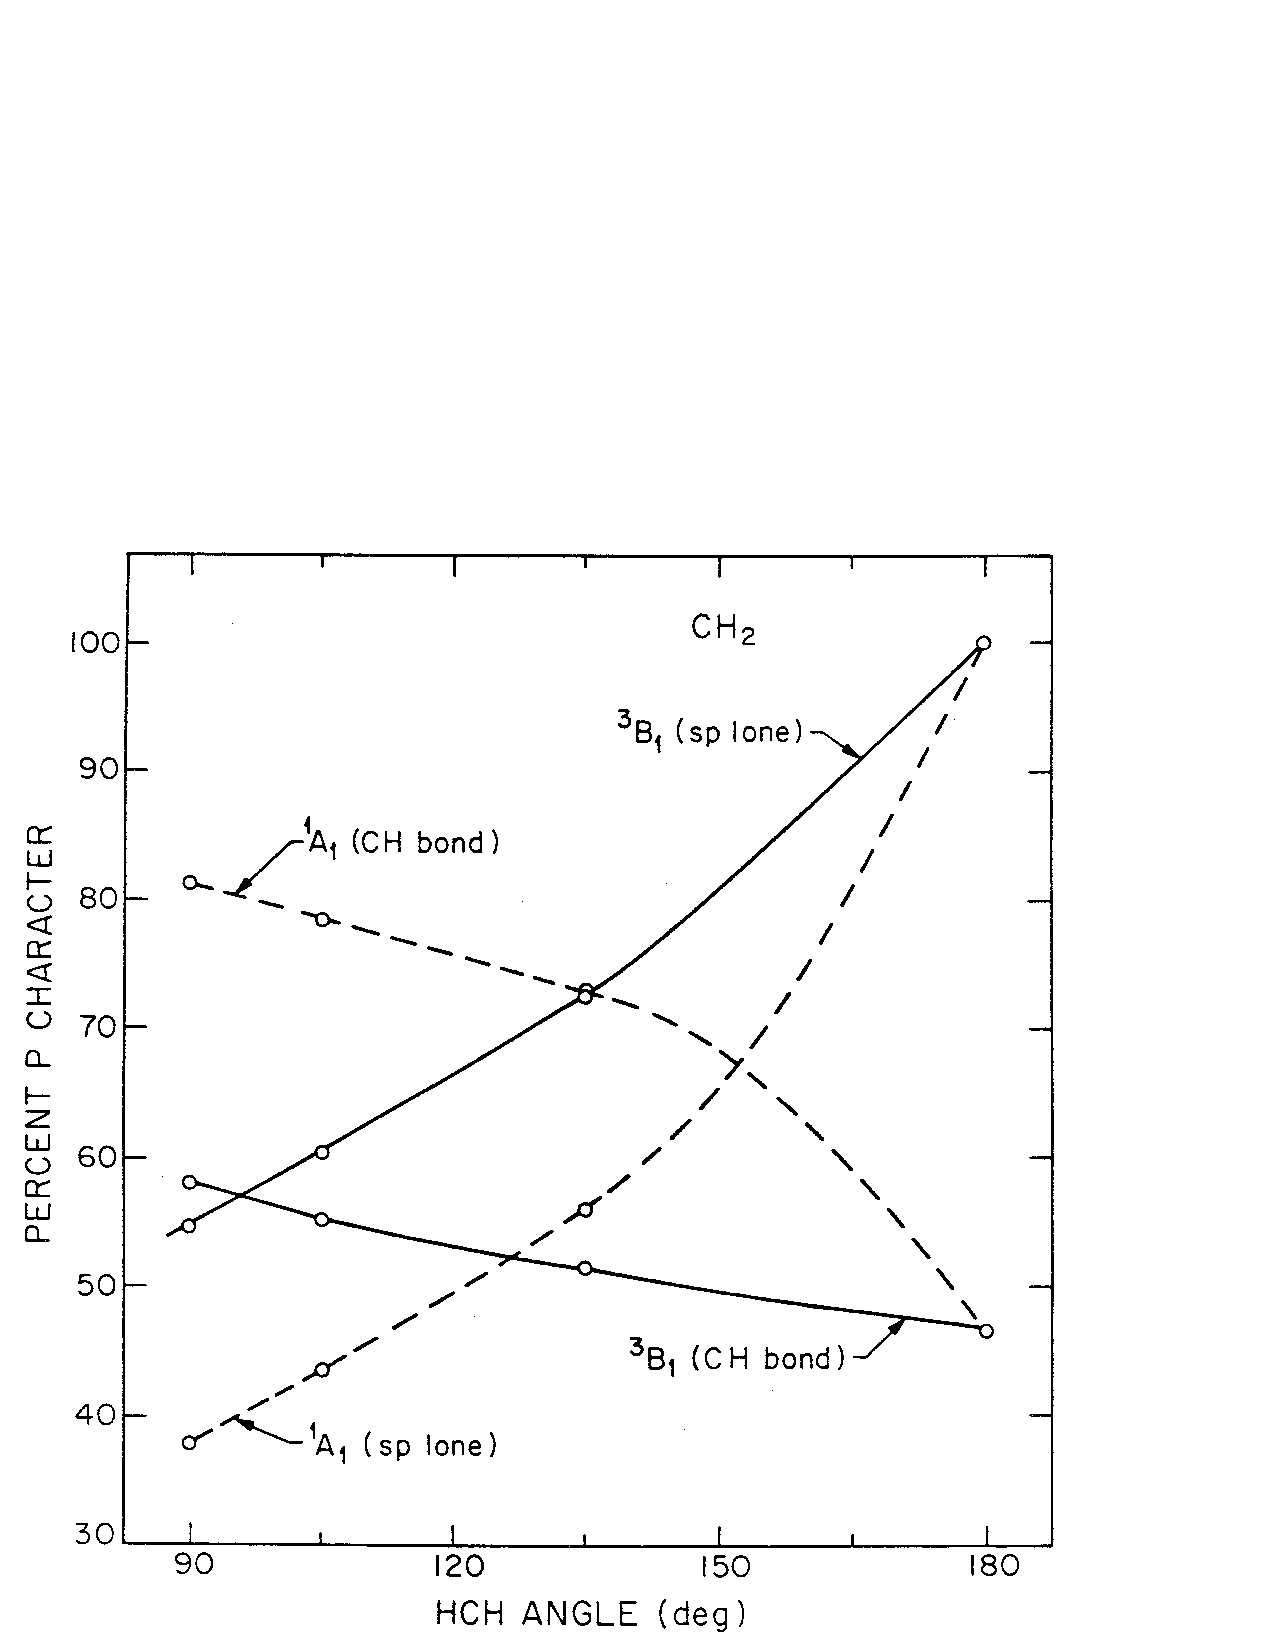
\includegraphics[scale=0.75]{fig6-10}
\caption{Hybridization of the GVB orbitals of CH$_2$.$^{12}$}
\label{chap6-fig11}
\end{figure}

\begin{table}
\caption{Hybridization of GVB orbitals.}
\label{chap6-table2}
\begin{center}
\begin{tabular}{ccccccc}\\ \hline

Molecule & Pair &\multispan2 \hfill Percent $p$ Character\hfill\cr
& & MBS$^a$ & DZ$^b$\cr

C(${^3P}$) & lone ($\sigma$) & 13.2 & 13.2\cr
CH(${^2\Pi}$) & bond & 92.8 & 81.5\cr
& lone ($\sigma$) &21.3 & 25.7\cr
CH(${^4\Sigma}^-$) & bond & 37.6 & 34.8\cr
& lone ($\sigma$) & 37.9 & 34.8\cr
CH$_2$(${^1A}_1$) & bond & 86.1 & 78.5\cr
& lone (sp) & 36.1 & 43.2\cr
CH$_2$(${3B}_1$) & bond & 51.9 & 51.5\cr
& lone (a$_1$) & 70.9 & 72.4\cr
CH$_2$(${^1B}_1$) & bond & 46.5 & 47.2\cr
& lone (a$_1$) & 82.8 & 83.8\cr
CH$_3$ & bond & 59.8 & 60.8\cr
CH$_4$ & CH bond & 53.2 & - \cr
& CH bond & 42.9 & 52.2\cr
C$_2$H$_4$ & CH bond & 74.4 & -\cr
& CC bond & 68.0 & -\cr
CH$_2$H$_6$ & CH bond & 68.5 & -\cr
& CC bond & 66.3 & 72.0\cr
CH$_3$H$_6$ & CC bond & 81.7 & -\cr
\hline
\end{tabular}
\end{center}
$^a$MBS = minimum basis set.

$^b$DZ = double zeta basis set.
\end{table}

\subsection{Low-Lying States of NH$_n$}

The ground state of N, consists of three singly-occupied $p$ 
orbtials.  Bonding an H to one of these, leads directly to the 
${^3\Sigma}^-$ state of NH,
\begin{equation}
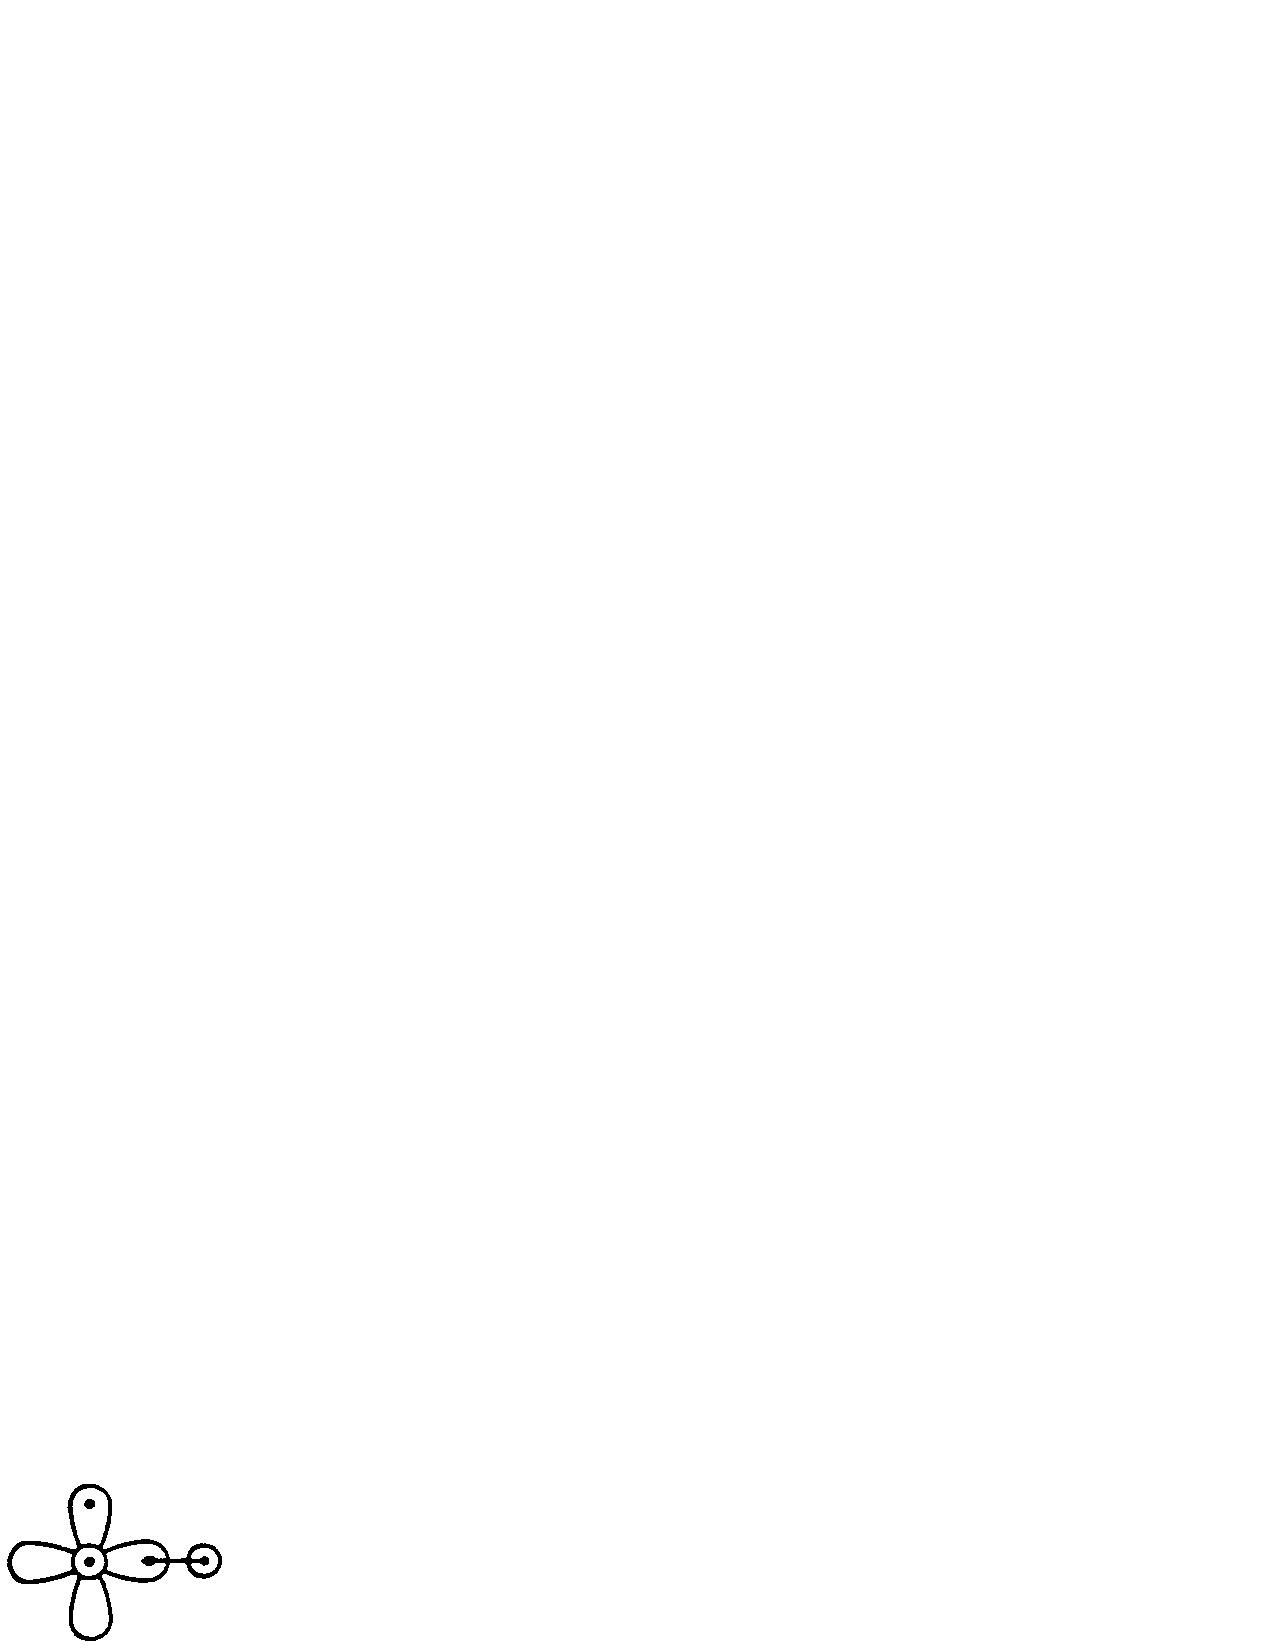
\includegraphics{fig6-10a}
\end{equation}
No other states, of NH, correlate with ground state atoms.

Starting with the ${^3\Sigma}^-$ state of NH, and bonding an H to one
of the two-singly-occupied $p \pi$ orbitals, leads to the ${^2B}_1$
state of NH$_2$
\begin{equation}
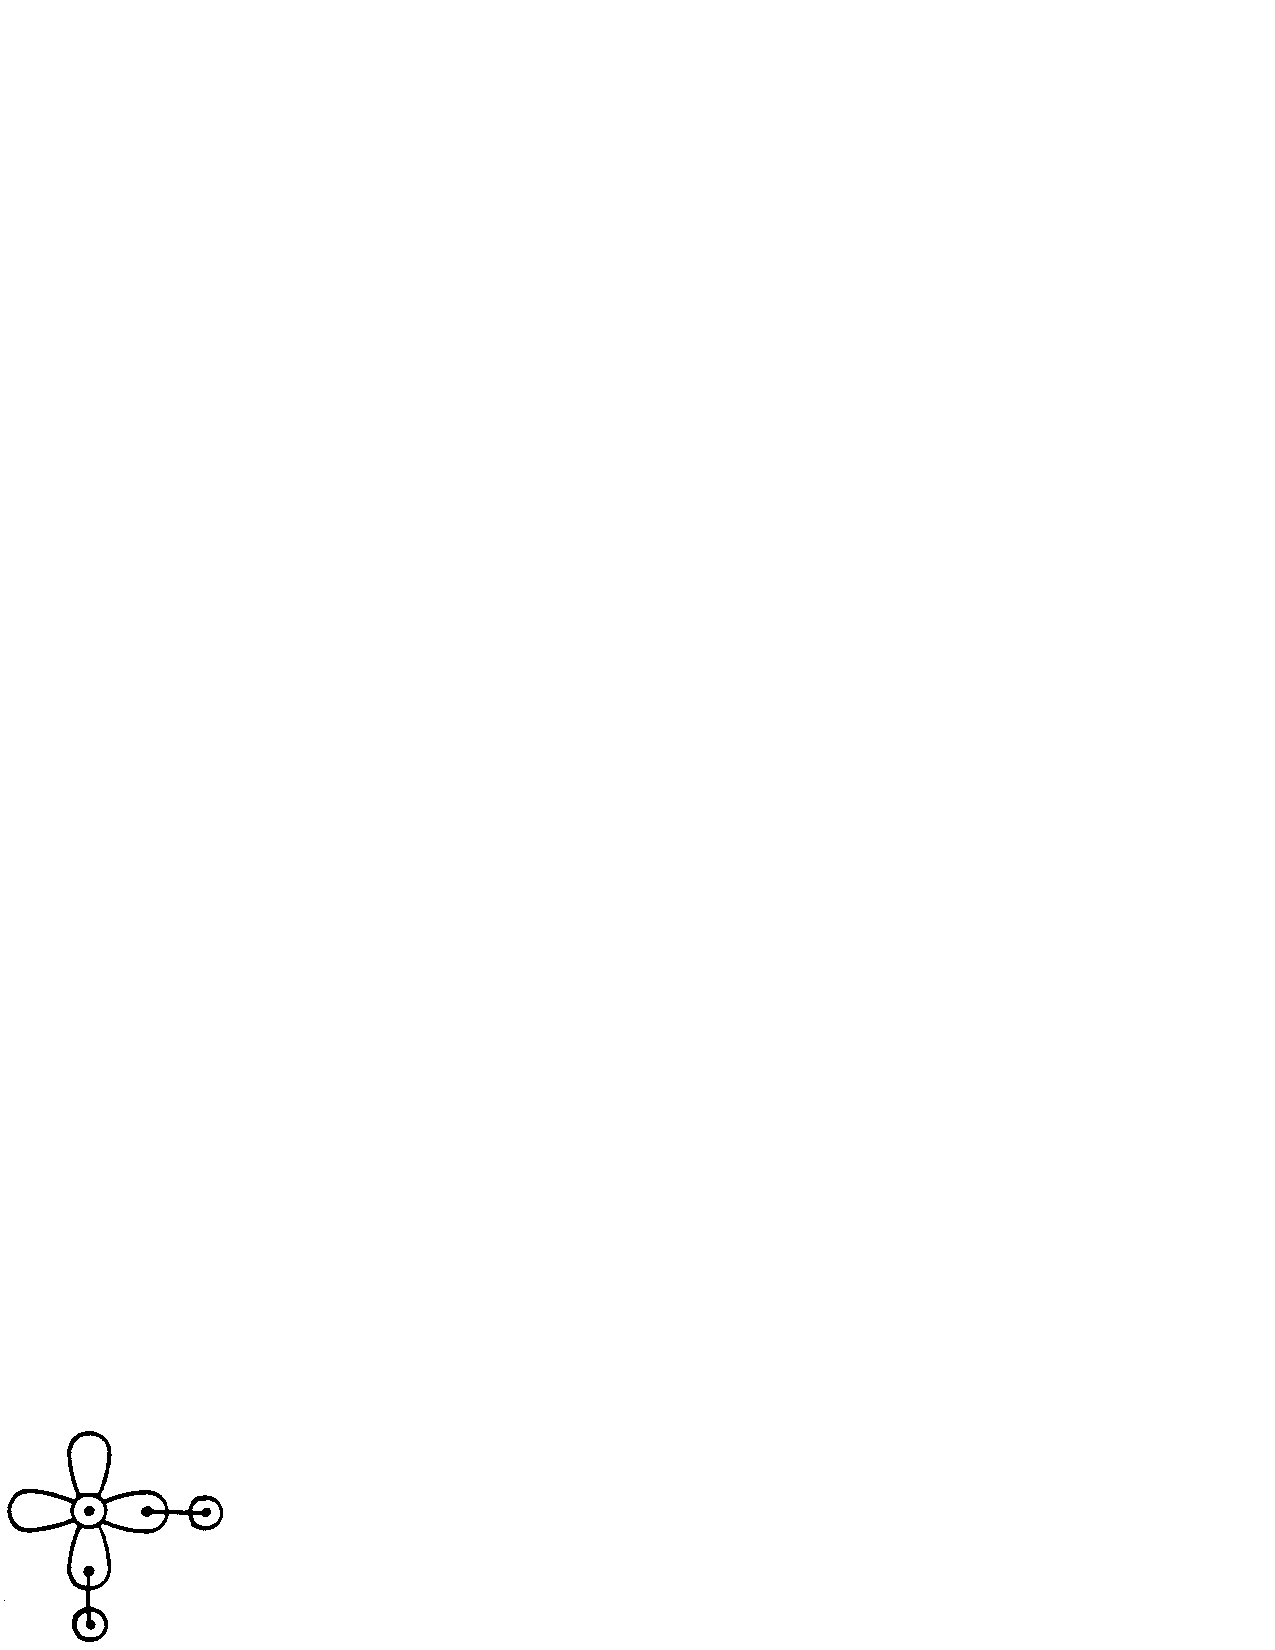
\includegraphics{fig6-10b}
\end{equation}
Bond-bond repulsions increase the bond angle to 103$^{\circ}$, to be 
compared with an optimum angle of 90$^{\circ}$ for PH$_2$.

Bonding the third H to (\ref{chap6-eqno30}), leads to pyramidal
NH$_3$, just as for PH$_3$.  However, the barrier to inversion in the
first-row compound, 6 kcal, is much smaller than that of the
second-row compound, approximately 37 kcal.  The reasons are that:
\begin{enumerate} 
\item The planar intermediate in the inversion
\begin{equation}
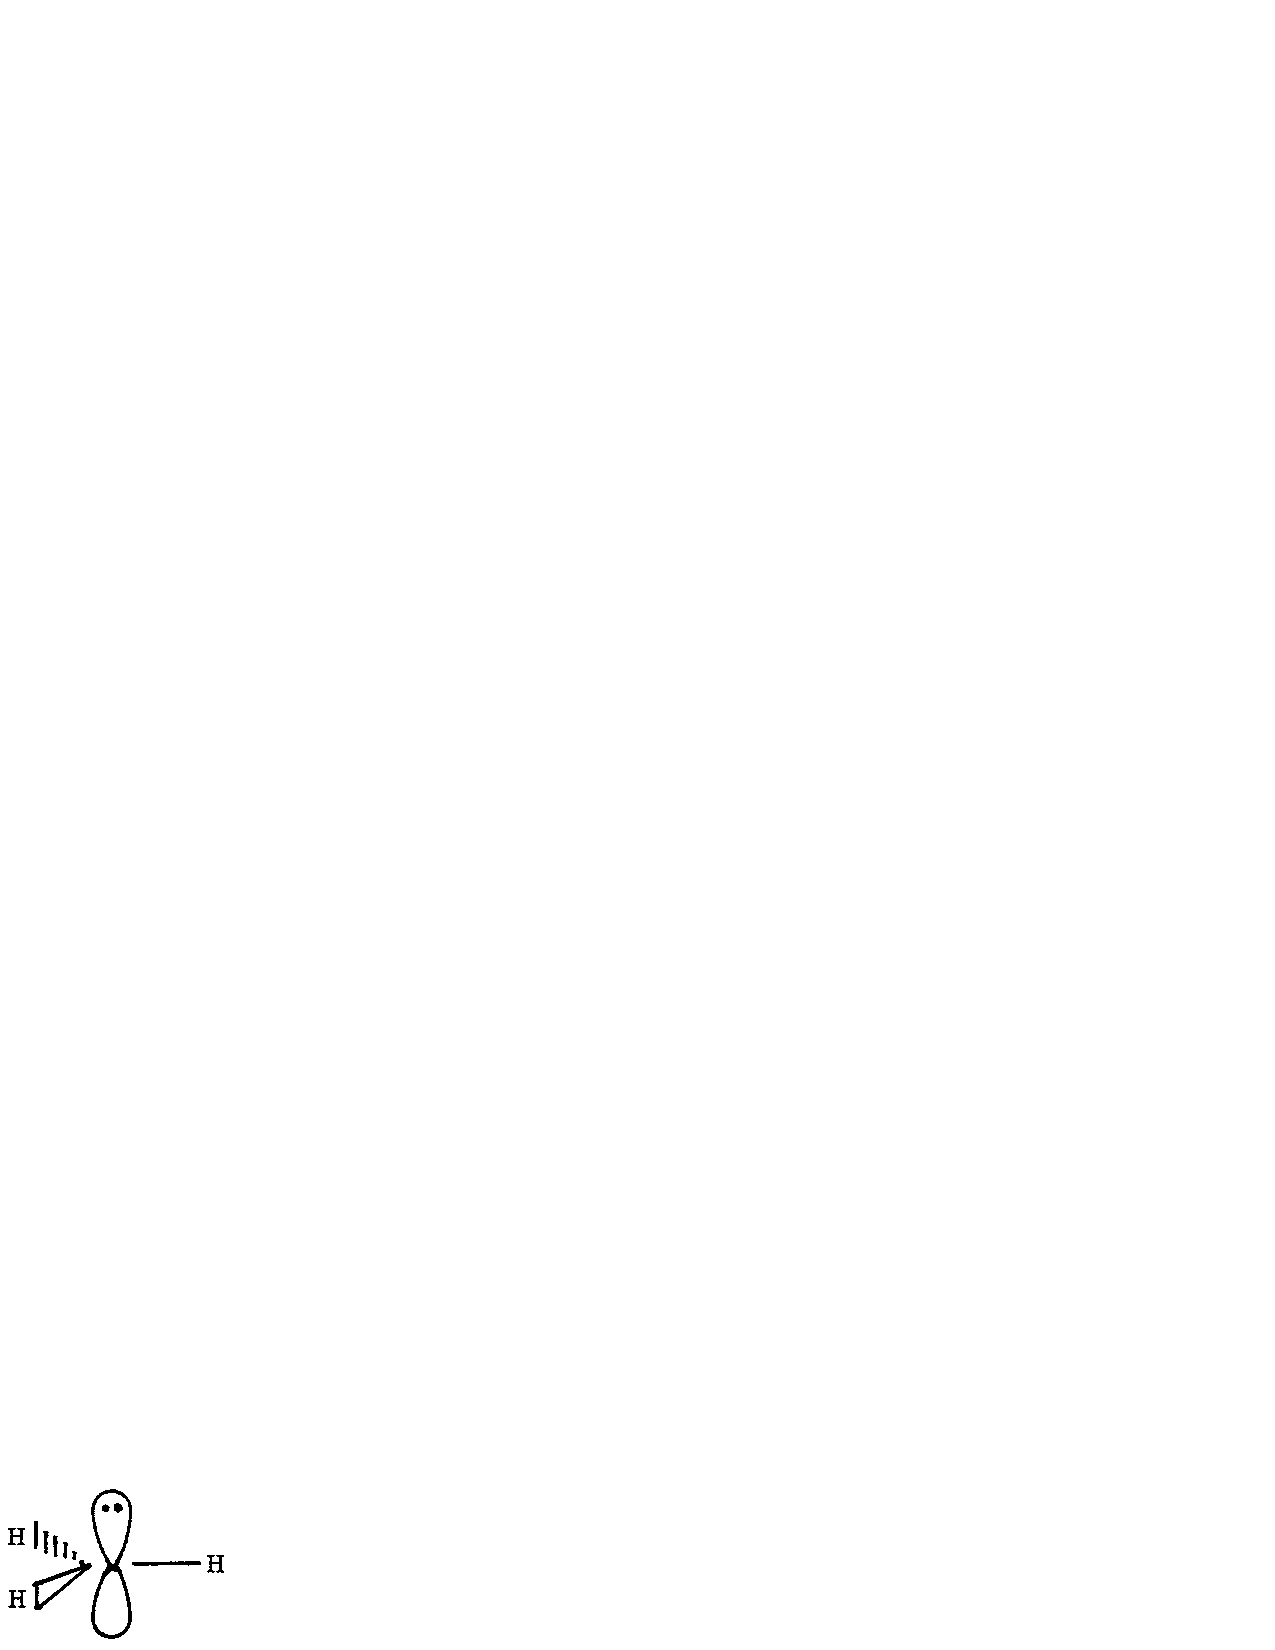
\includegraphics{fig6-10c}
\end{equation}
requires two lobe bonds plus a $p$ bond, as compared with three $p$ 
bonds for pyramidal.  For P, the lobe bond is much weaker than the $p$ 
bond, leading to a very large barrier, whereas in N these bonds are 
more comparable.  

\item Because of the greater bond-bond 
repulsion in NH$_3$, the ground state is distorted toward the planar 
intermediate, leading to a decreased barrier.
\end{enumerate}
\section{Halides}

Since the valence shell of fluorine and other halogens ($ns^2np^5$) 
contains only singly-occupied orbital, we expect the compounds AX$_n$ 
to be qualitatively similar to the corresponding AH$_n$ molecules.  
There are, however, two important differences to be considered.  
First, the large electronegativity of the halogens, and second, the 
interaction of the doubly-occupied valence orbitals of the halogen 
with adjacent centers.  In this section, we discuss briefly the 
implications of these effects on the electronic structure of simple 
halides, using the CX$_n$ series to illustrate the concepts.

Bonding the singly-occupied $2p$ orbital of an F, to a $p$ orbital of 
atomic C, leads directly to the ${^2\Pi}$ ground state of CF,
\begin{equation}
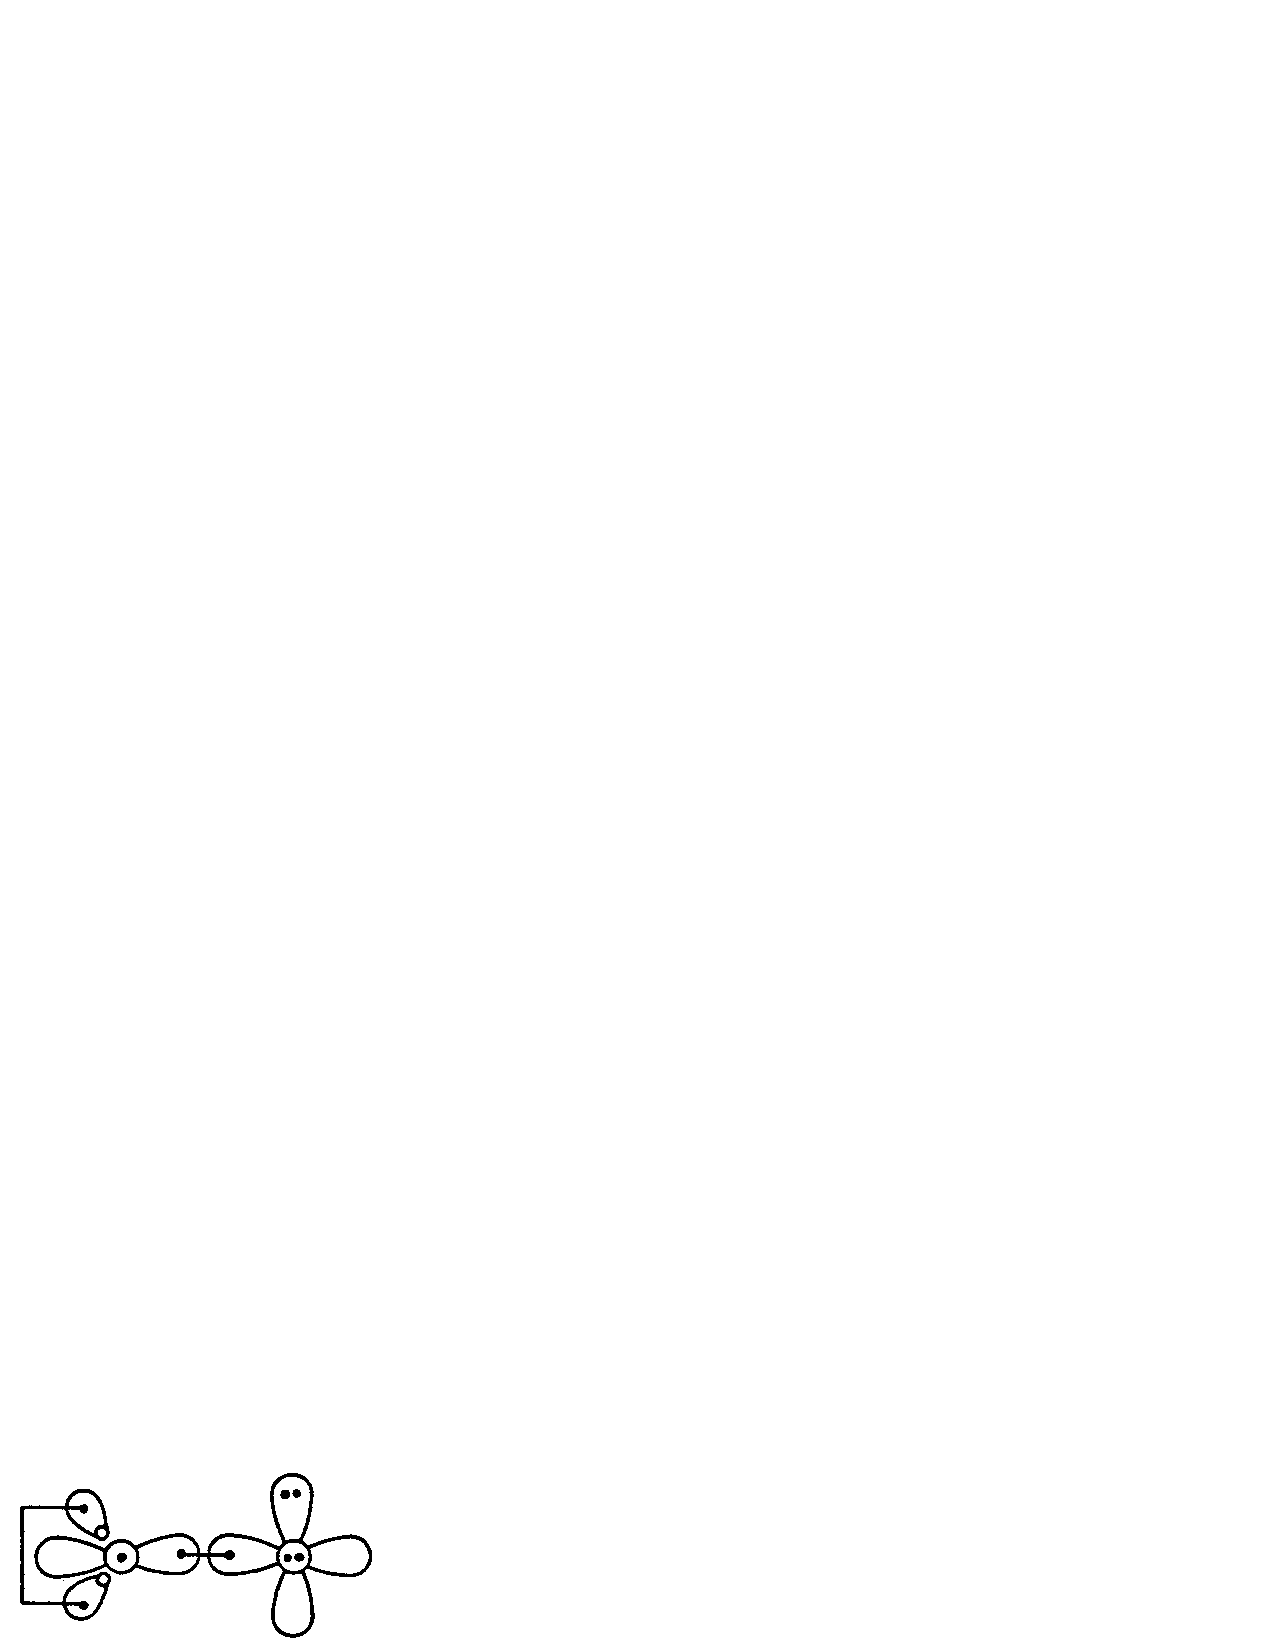
\includegraphics{fig6-10d}
\label{chap6-eqno32}
\end{equation}
Similarly, bonding to a lobe orbital of C leads to the ${^4\Sigma}^-$ 
state,
\begin{equation}
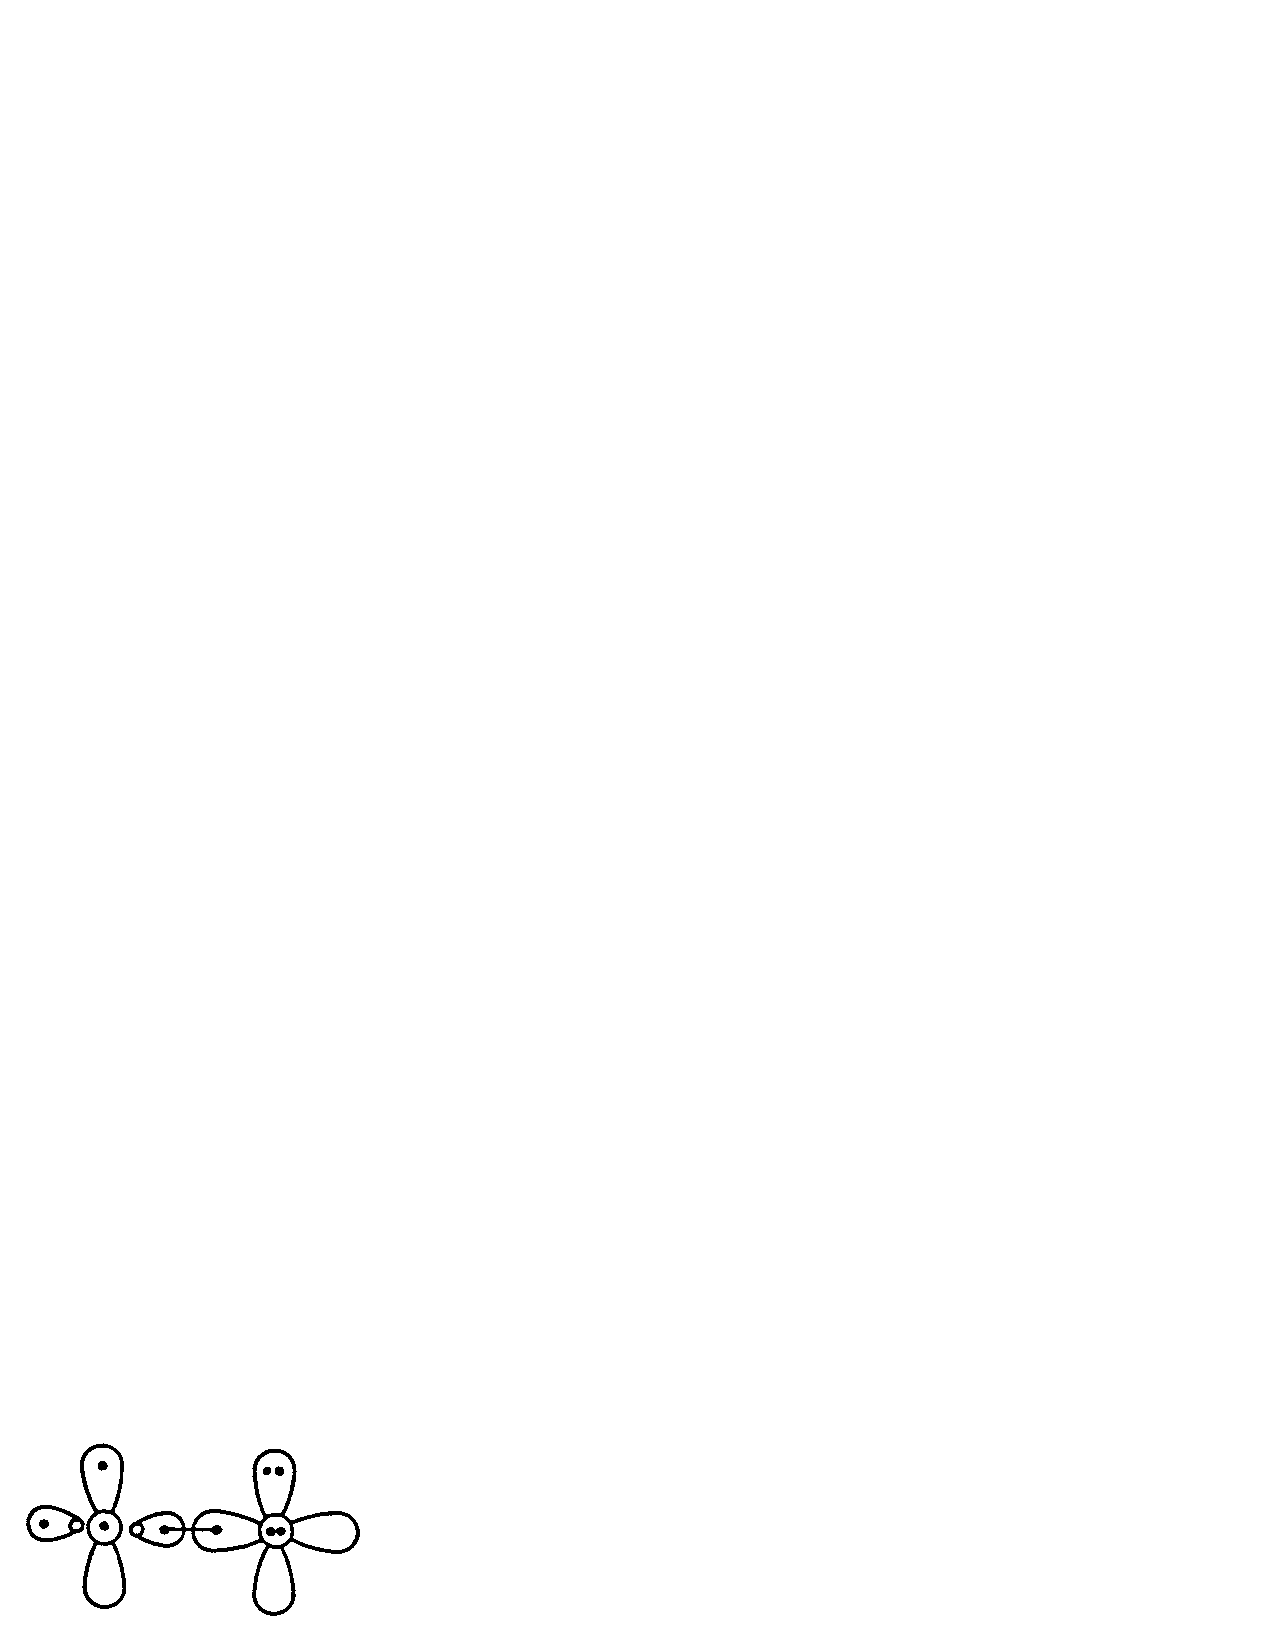
\includegraphics{fig6-10e}
\end{equation}
For CH, the bond energy of the ${^2\Pi}$ state is 80 kcal, while 
that of the ${^4\Sigma}^-$ state is only slightly less, 63 kcal, and 
hence, the CH($^{2\Pi} - {^4\Sigma}^-$) separation is 17 kcal.  
Consider now the effect of replacing the covalent bond of C-H with a 
highly ionic bond polarized away from the carbon.  In order to 
estimate the bond energy of C$^+$F$^-$, consider the cycle:
\begin{enumerate}
\item Start with C and F atoms separated by a distance $R$.  
\item Ionize C atom leading to C$^+$.  
\item Add this electron to F, leading to F$^-$.  
\item Consider the long-range $1/R$ attraction of these two 
changes.  
\end{enumerate}
The net energy charge is
\begin{equation}
\Delta E = \mathrm{IP(C)} - \mathrm{EA(F)} - {1 \over R},
\end{equation}
and hence, the bond energy is
\begin{equation}
D_\mathrm{ION} (C^+F^-) = \mathrm{EA(F)} - \mathrm{IP(C)} + {1 \over R}.
\label{chap6-eqno33}
\end{equation}
The $1/R$ is for atomic units.  If $R$ is in \AA\ and $D$ is in eV,
replace $1/R$ by $14.3998/R$, and if $D$ is in kcal, replace $1/R$ by
$332.059/R$.  The formula (\ref{chap6-eqno33}) is not correct when the
atoms are close enough for the orbitals to overlap; however, we will
use it anyway.  An important point here is that the $OP(C)$ depends on
the molecular state.  For example, in this idealized model, the
${^2\Pi}$ state of CF is described as
\begin{equation}
C^+ \left( 2s^2 2p^1 \right) F^- \left( 2s^2 ep^6 \right),
\end{equation}
while the ${^4\Sigma}^-$ state is of the form
\begin{equation}
C^+ \left( 2s^1 2p^2 \right) F^- \left( 2s^2 ep^6 \right).
\end{equation}
Thus, the appropriate ionization potentials, IP, are
\begin{equation}
\mathrm{IP}_{2p} (C) = 260 ~ {\rm kcal}
\end{equation}
for the ${^2\Pi}$ state, and
\begin{equation}
\mathrm{IP}_{2s} (C) = 383 ~ {\rm kcal}
\end{equation}
for the ${^4\Sigma}^-$ state.  Substitution into (33), using $R = 
1.27$ \AA, leads to the following bond energies,
\begin{equation}
D_\mathrm{ION} \left( {^2\Pi} \right) = 78 - 260 + 261 
= 79 ~ {\rm kcal},
\end{equation}
and
\begin{equation}
D_\mathrm{ION} \left( {^4\Sigma}^- \right) = 78 - 383 + 261 
= - 43 ~ {\rm kcal}.
\end{equation}
Thus, the ionic bond energy of the ${^2\Pi}$ state is comparable to 
the covalent bond energy of CH, 80 kcal, which is presumably close to 
the covalent bond energy in CF(${^2\Pi}$).  These two idealized 
structures, covalent and ionic, overlap considerably, and hence, the 
actual wavefunction of CF(${^2\Pi}$) will be a combination of the 
two, leading to a bond energy lower than either.  The actual bond 
energy of CF(${^2\Pi}$) is 127 kcal.

Consider now, the ${^4\Sigma}^-$ state, the estimated ionic bond 
energy is much less favorable, in fact, it is negative.  Therefore, 
we do not expect a significant contribution of the ionic structure in 
the optimum wavefunction.  In fact, the bond energy of 
CF(${^4\Sigma}^-$) is approximately 63 kcal,$^{19}$ quite close to 
that of the covalent molecule CH(${^4\Sigma}^-$), 63 kcal.

Consider now, bonding a second F to C, form CF$_2$.  Starting with the
${^2\Pi}$ state of CF, (\ref{chap6-eqno32}), there are again two
possibilities.
\begin{enumerate}
\item CF$_2$(${^1A}_1$), in which the second bond is 
to the unpaired $p$ orbital of CF,
\begin{equation}
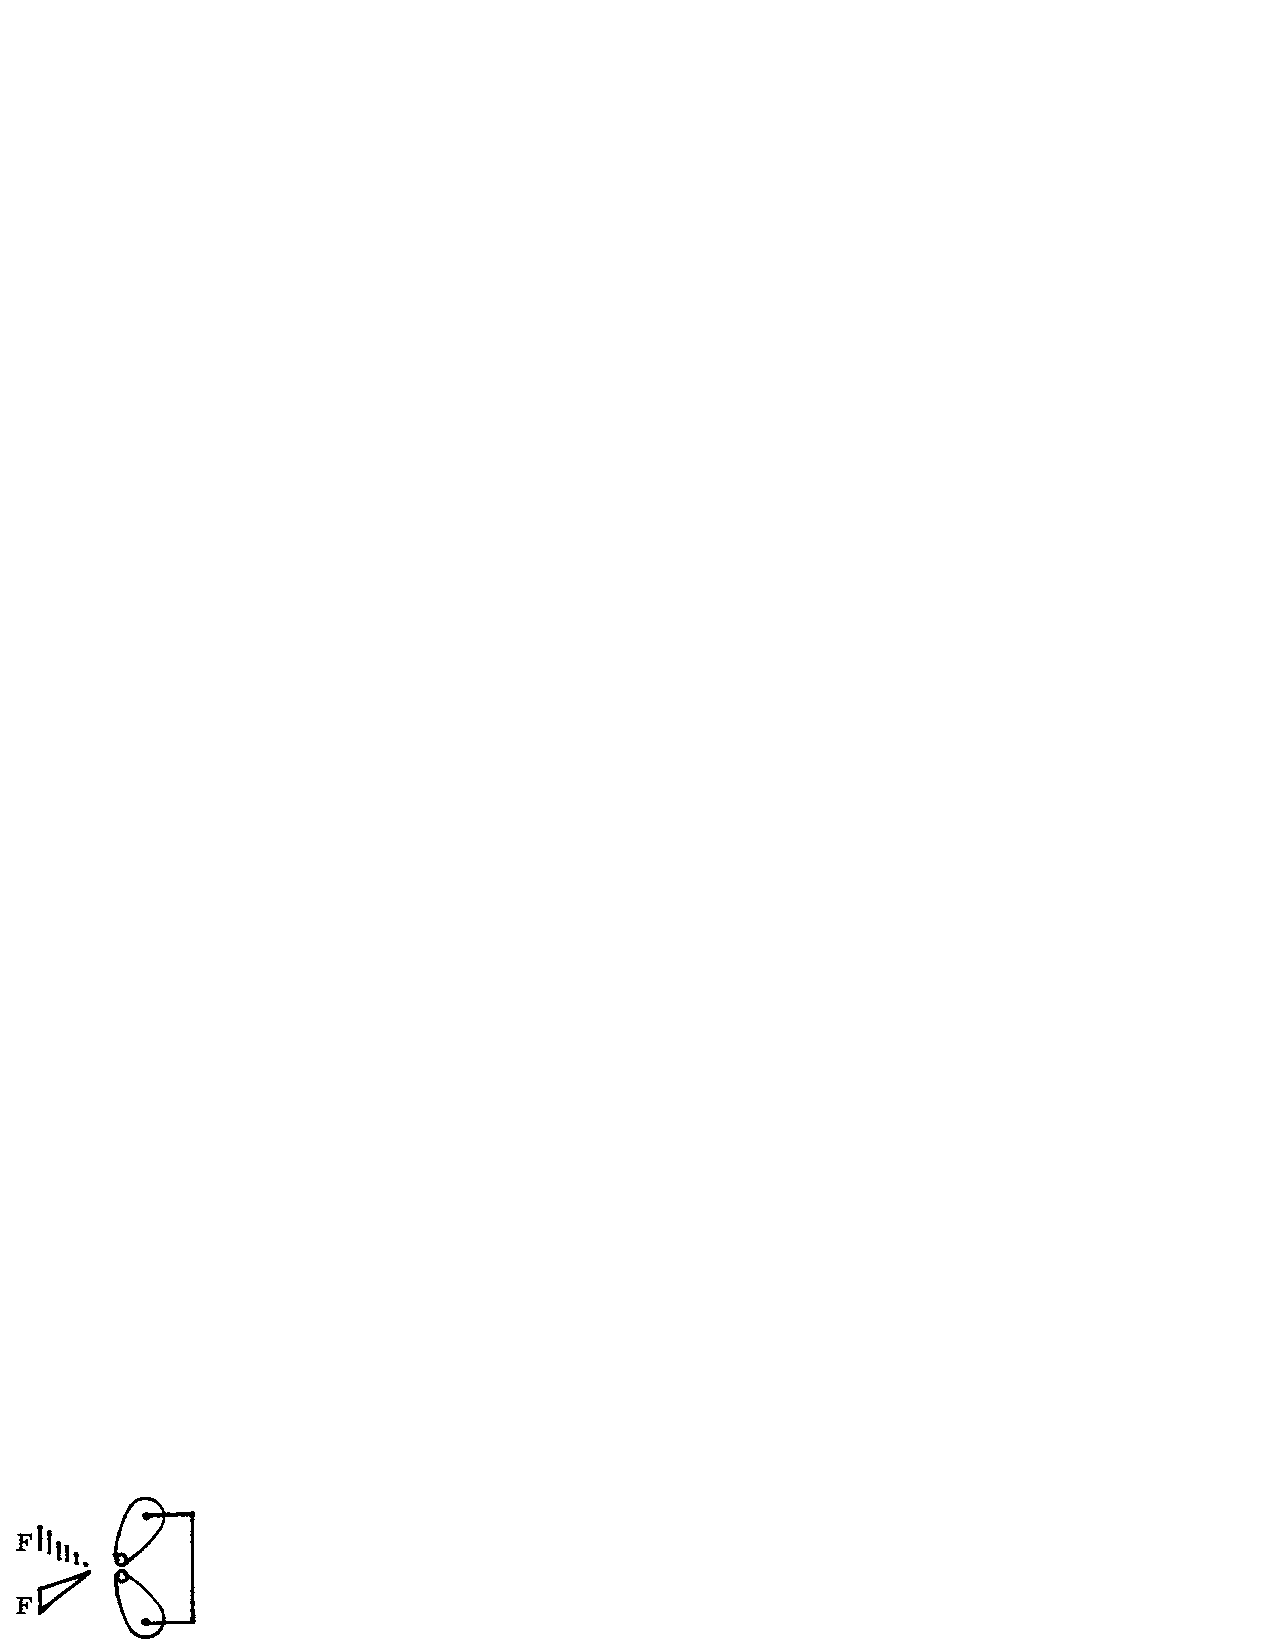
\includegraphics{fig6-10f}
\label{chap6-eqno34}
\end{equation}
\item CF$_2$(${^3B}_1$), in which the bond is to a lobe orbital,
\begin{equation}
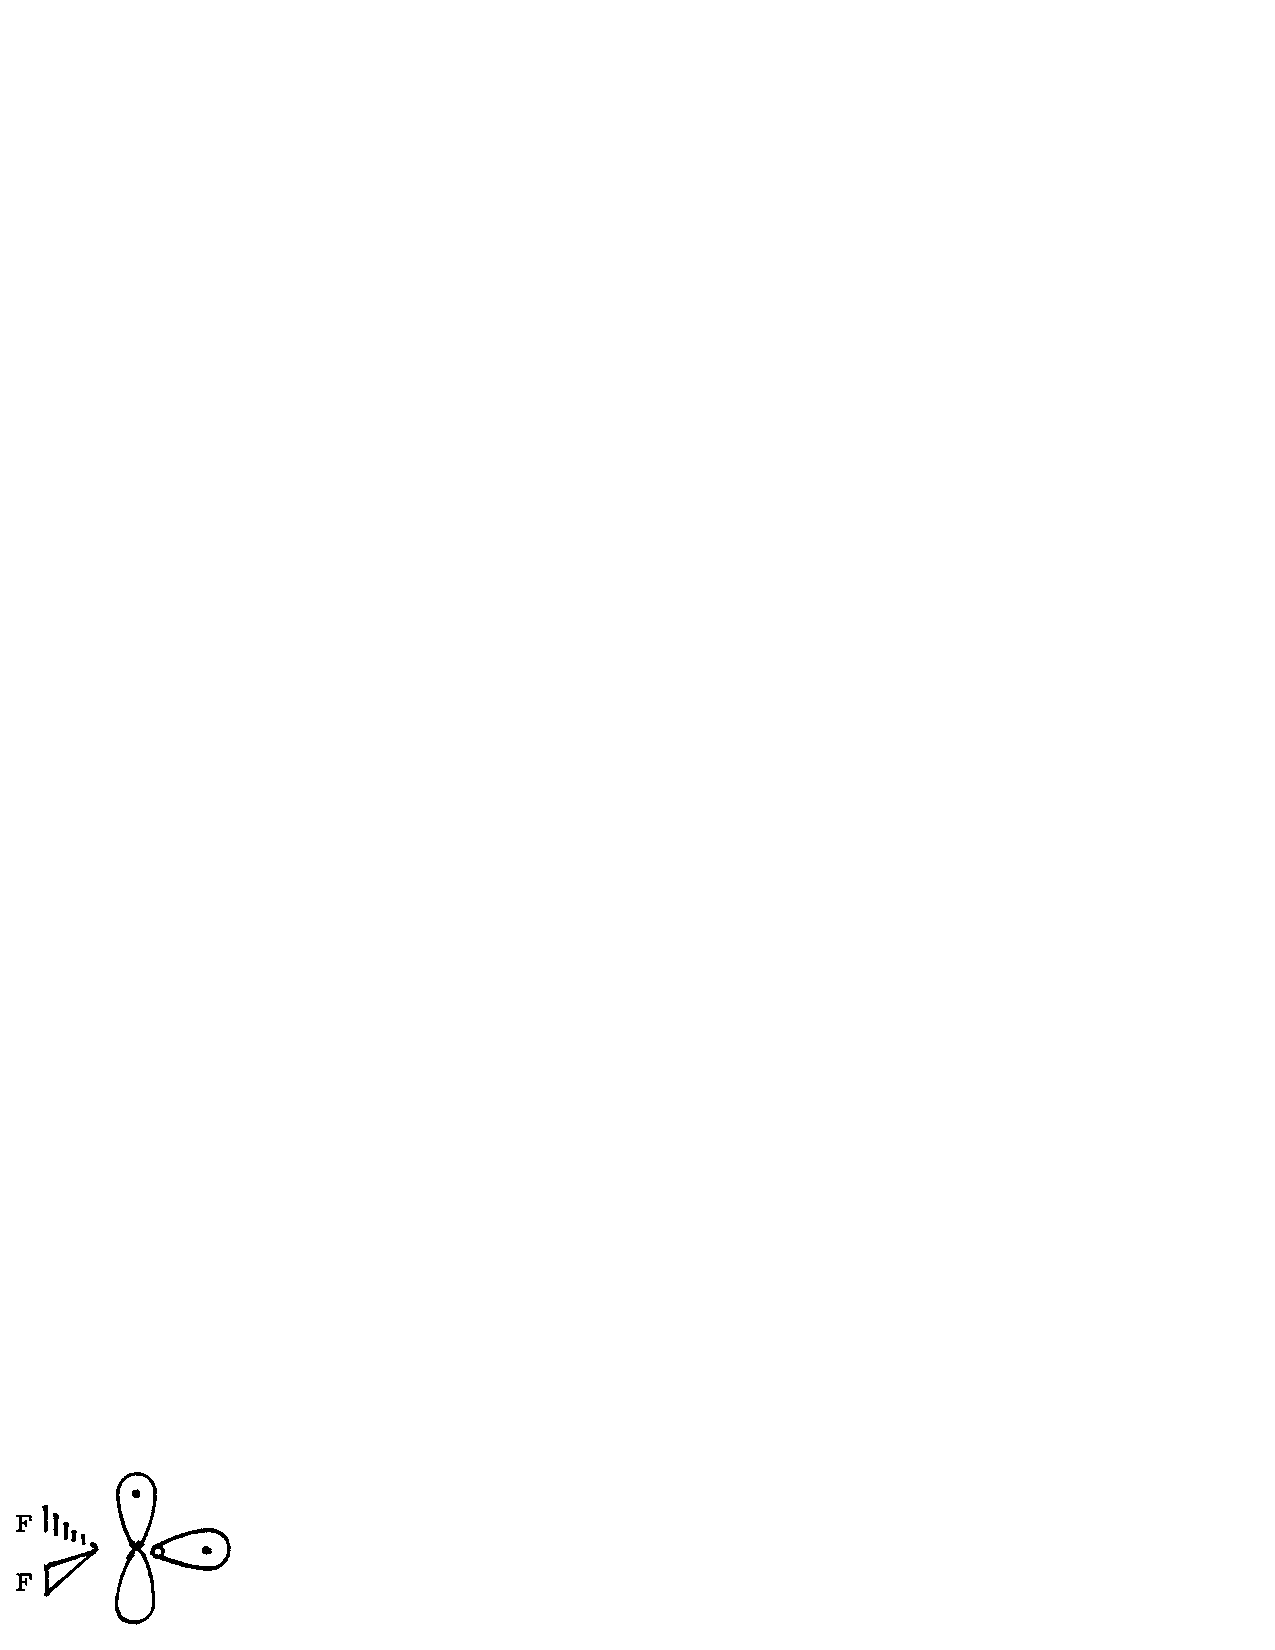
\includegraphics{fig6-10h}
\end{equation}
\end{enumerate}
For the hydride, these two state are of comparable energies, the 
${^3B}_1$ state is 9 kcal below the ${^1A}_1$.  For CF$_2$, the above 
arguments suggest that the second F will bond much more strongly to a 
$p$ orbital than a lobe as found for CF, and hence, that the ground 
state of CF$_2$ is the  ${^1A}_1$ state.  In fact, the ${^3B}_1$ state 
of CF$_2$ lies approximately 46 kcal above the ${^1A}_1$ state.$^{20}$

Starting with CF$_2$( ${^1A}_1$), (\ref{chap6-eqno34}), and bonding a
third F, there is only one choice, a bond to a lobe orbital of CF$_2$.
This third bond will then be
\begin{equation}
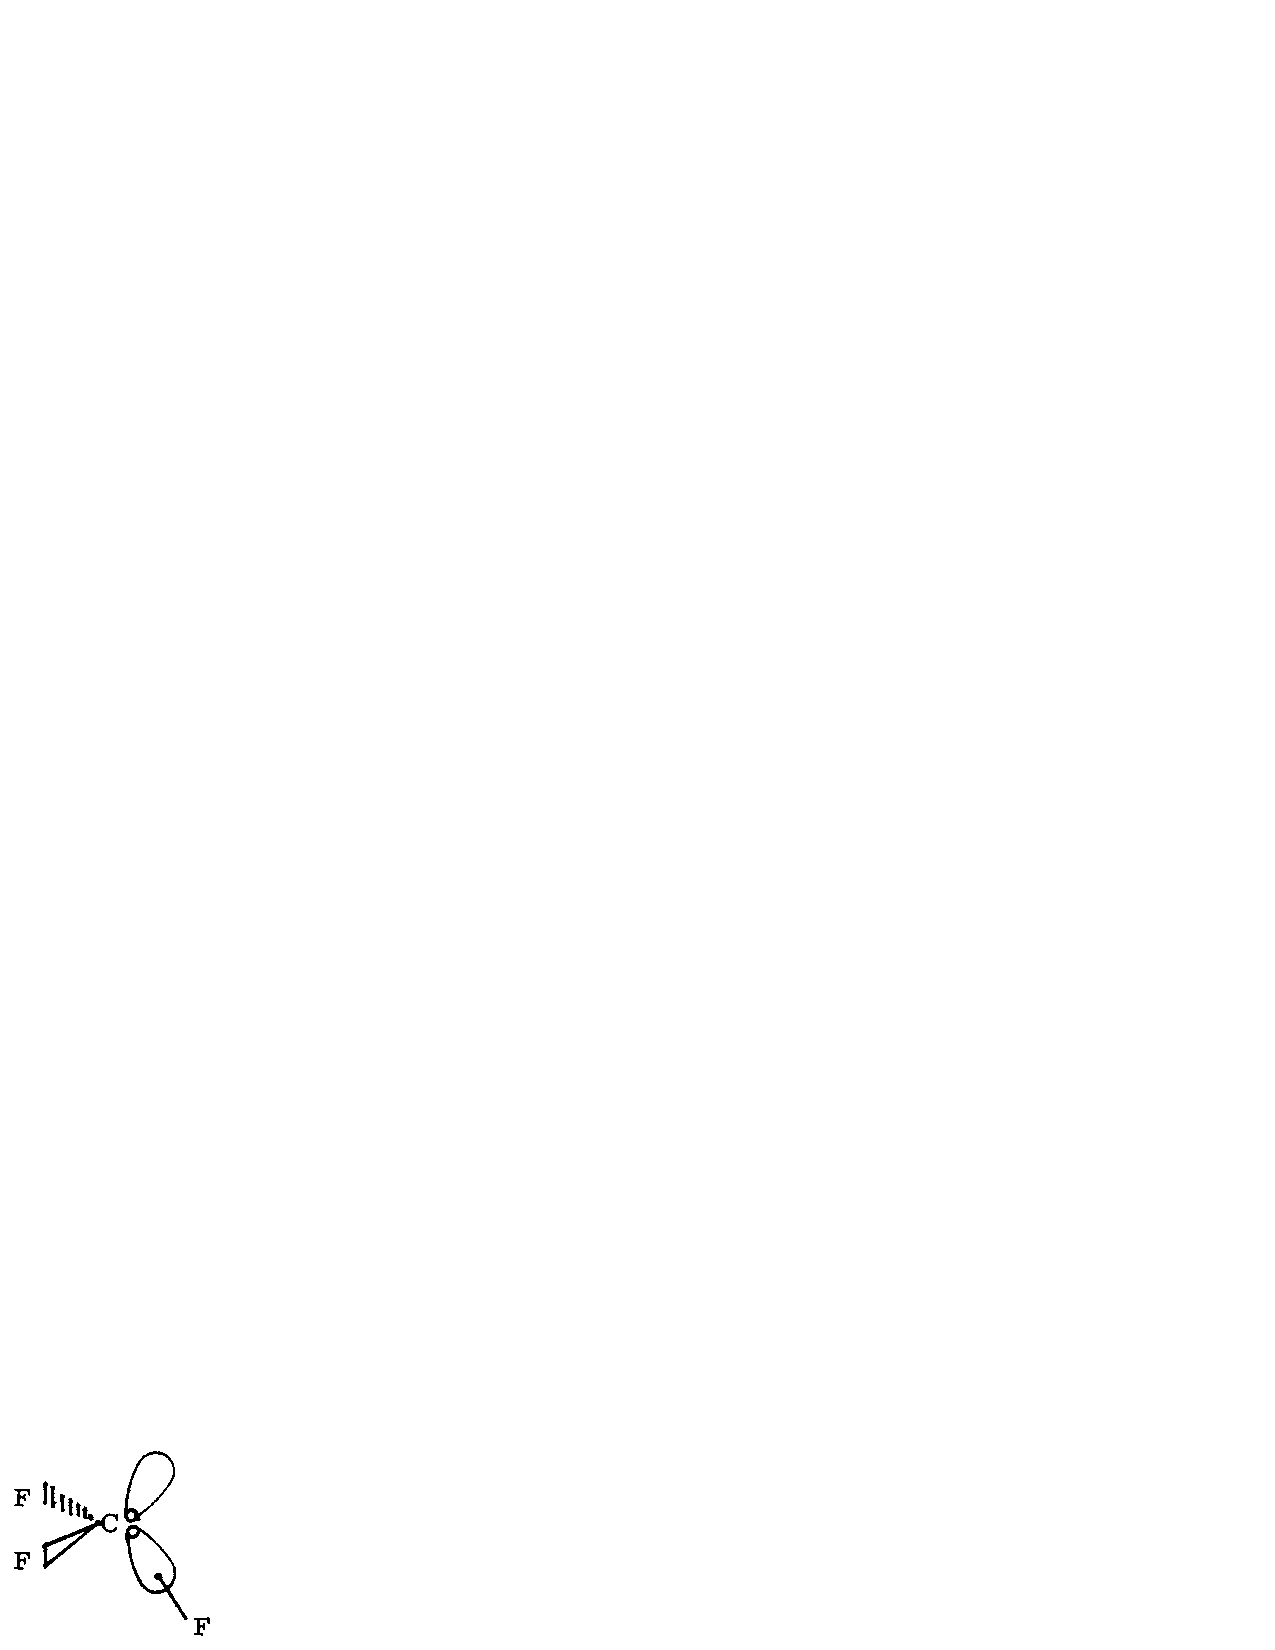
\includegraphics{fig6-10g}
\end{equation}
much weaker than either of the first two, since the lobe orbitals of 
CF$_2$ must be unpaired, and since the bond involves a lobe of C 
rather than a $p$ orbital, hence, ionic character will not be an 
important factor.  The result is pyramidal CF$_3$, thereby maximizing 
the carbon $p$ character in the bonds.  This is in contrast to CH$_3$ 
which, as discussed earlier, is planar.

In summary, the ionization potential of a valence $p$ orbital is 
always much smaller than that of a valence $s$ orbital.  Consequently, 
in considering the bonding between two atoms of very different 
electronegativities, such as C and F, bonds involving a $p$ orbital 
of the less electronegative atom will be much more stable than those 
involving lobe orbitals, due to the incorporation of ionic character in 
the $p$ orbital bond.  Thus, comparing the CH$_n$ molecules to CF$_n$ 
series, the large difference in electronegativities of H and F, lead 
to important differences in the electronic structure and geometries 
of these species.

Consider now, the remaining halogens, Cl, Br, I, and At.  An important
difference between F, and all the lower halogens, is that bond
distances become much longer as we move down the row of halogens.
Consequently, the $1/R$ term of (\ref{chap6-eqno33}) is not nearly as
favorable.  Thus, even for Cl, which has a higher electron effinity
than F, ionic bonding character will not be as important.  As a
result, for Cl, Br, I, and At, the relative bond strengths to $p$ and
lobe orbitals are more comparable.  In addition, the total bond
strength of the ${^2\Pi}$ state of CX, becomes much smaller, 128, 95,
67, and 50 kcal for CF, CC, CBr, and CI, respectively.  Similarly, the
${^2\Pi} - {^4\Sigma}^-$ separation should decrease along this series.

For CX$_2$, as the importance of ionic bonding decreases, the energy 
of the ${^1A}_1$ state will increase relative to the ${^3B}_1$ state.  
For example, the ${^1A}_1 - {^3B}_1$ separation of CCl$_2$ is only 13 
kcal, compared with a separation of 46 kcal for CF$_2$.$^{20}$  In 
fact, for CBr$_2$ or CI$_2$, the ${^3B}_1$ state may well be the 
ground state.  Replacing the electronegative halogen with an 
electropositive alkali, reverses these trends, favoring 
${^4\Sigma}^-$ CNa, and ${^3B}_1$ CNa$_2$.

Consider now, replacing the carbon in the CX$_n$ seires with one of
its lower row analogues, Si or Ge.  There are two important
differences to be considered.  First, the absolute ionization
potentials are much smaller.  For example, $IP_p = 260$, 188, and 182
kcal for C, Si, and Ge, respectively.  Second, the bond lengths
becomes larger, R$_e$(C-F) = 1.272, R$_e$(Si-F) = 1.601.  Taking
CF-SiF as a specific comparison, substitution into
(\ref{chap6-eqno33}) leads to an ionic bond strength for the ${^2\Pi}$
state of SiF of 97 kcal.  For comparison, the corresponding covalent
bond strength, SiH, is 71 kcal, and the observed bond strength of SiF
is 129 kcal.  Thus, we see that the large decrease in the atomic
ionization potentials of the lower rows of the periodic charge, leads
to an increased importance of ionic character in the halides of these
elements.  Thus, the bonding in second-row halides will be similar to
that discussed for the CX$_n$ series.

\section{Bond Energies}

In the preceding sections, we presented an orbital description of 
the electronic structure of simple hydrides and halides. In this 
section, we discuss the trends in bond energies that can be understood 
in these terms.

Consider the ground states of $P({^4S})$, $PH({^3\Sigma}^-)$, 
$PH_2({^2B}_1)$, and $PH_3 ({^1A})$.  Each bond, in this series, involves 
a singly-occupied $3p$ orbital of phosphorus. Thus, one might expect the three
bond energies to be comparable, possibly decreasing slightly due to
bond-bond repulsions. In fact,the trend should be in the opposite direction,
\begin{equation}
D(\mathrm{P-H}) < D(\mathrm{HP-H}) < D(\mathrm{H_2P-H}),
\end{equation}
with an increase of 5 kcal per H.  In order to understand this trend, 
we must consider the $p-p^{\prime}$ exchange
interactions in each of these molecules.

Assuming each bond pair to be purely covalent, the energies of these 
molecules have the form
\begin{eqnarray}
E [ \mathrm{P}({^4S}) ] &=& E_0 (\mathrm{P}) - K_{xy} - K_{xz} - K_{yz}\cr
E [ \mathrm{PH}({^3\Sigma}^- ) ] &=& E_0(\mathrm{PH}) - K_{xy} - {1
  \over 2} K_{xz} - {1  \over 2} K_{yz}\cr
E [ \mathrm{PH}_2 ( {^2B}_1 ) ] &=& E_0 ( \mathrm{PH}_2 ) - {1 \over
  1} K_{xy} - {1  \over 2} K_{xz} - {1 \over 2} K_{yz}\cr
E [ \mathrm{PH}_3 ( {^1A} ) ] &=& E_0 ( \mathrm{PH}_3 ) - {1 \over 2}
K_{xy} - {1 \over  2} K_{xz} - {1 \over 2} K_{yz},
\end{eqnarray}
where we have considered explicitly only the one center $p-p^{\prime}$ 
exchange integrals.   Assuming the exchange-less bond energies, 
$D_{PH}$ to be constant, neglecting bond-bond interactions, 
leads to the predicted bond energies,
\begin{eqnarray}
D ( \mathrm{H_2P-H}) &=& D_\mathrm{PH}\cr
D ( \mathrm{HP-H}) &=& D_\mathrm{PH} - {1 \over 2} K_{xy}\cr
D ( \mathrm{P-H}) &=& D_\mathrm{PH} - {1 \over 2} K_{xz} - {1 \over 2} K_{yz}.
\end{eqnarray}
Using the experimental atomization energy for the saturated AH$_3$
molecules and exchange integrals derived from atomic spectra leads to
the predicted bond energies of Table \ref{chap6-table3}.  In most
cases, the predicted energies are probably more accurate than the
current experimental data.

A similar analysis for the OH$_n$, SH$_n$, etc., series leads to
\begin{eqnarray}
D ( \mathrm{HA-H}) &=& D_\mathrm{AH}\cr
D ( \mathrm{A-H} ) &=& D_\mathrm{PH} - {1 \over 2} K_{xy}.
\end{eqnarray}
The numerical results are also given in Table \ref{chap6-table3}.
Again, all predictions are within experimental error limits except for
$D(O-H)$, which is 3 kcal high.

\begin{table}
\caption{Estimated bond energies and heats of formation, in kcal/mol,
of AH$_n$ species.} 
\label{chap6-table3}
\begin{tabular}{lcccccccc}\\ \hline
& N & P & As & Sb & O & S & Se & Te\cr

$\Delta 
H_{fo}(A)$&112.5$\pm$1&79.18$\pm$0.05&72.04&62.63&58.989$\pm$0.03
&66.14$\pm$0.5&54.11&47.0\cr
$\Delta 
H_{fo}(AH_m)$&-9.30$\pm$0.1&7.0$\pm$0.4&17.70&36.625&-57.103
&-4.18$\pm$0.15&8,05&24.8\cr
$K_{pp}$$^a$&18.32&10.84&10.29&8.88&22.57&12.93&12.34&12.0\cr
$D_{pH}$&101.39&81.11&74.89&64.74&115.32&90.03&77.75&69.7\cr
$D(A-H)$&83.07&70.27&64.60&55.86&104.04&83.56&71.58&59.7\cr
$D(H-AH)$&92.23&75.69&69.75&60.30&115.32&90.03&77.75&65.7\cr
$D(H-AH_2)$&101.39&81.11&74.89&64.74&-&-&-&-\cr
$\Delta 
H_{fo}$(AH)$^b$~Calc&81.06&60.54&59.07&58.40&6.58&34.21&34.17&38.9\cr
~~~~~~~~~~Exp$^a$&81.0$\pm$1.5&60.4$\pm$8.&-&-&9.35$\pm$0.04&34.4$\pm$4.&-&-\cr
$\Delta H_{fo}$(AH$_2$)~Calc&40.47&36.49&40.96&49.74\cr
~~~~~~~~~~Exp$^a$&40.8$\pm$3.&30.6$\pm$23.\cr
\end{tabular}
$^a$Based on lowest two LS states after averaging over J state.
\end{table}

The above analysis can be extended to include bonds to lobe orbitals, 
leading to relationships between excitation energies and inversion 
barriers of the various hydrides. This analysis, though, is beyond 
the scope of the present discussion.

In conclusion, the qualitative orbital view of molecules derived 
from {\it ab initio}, GVB, calculations of 
atoms, leads to simple concepts that can be used for semi-qualitative 
predictions of molecular geometries, bond energies, and order of 
electronic states.

\section{Potential Energy Curves and Higher Excited States}

In this section we will consider some additional excited states for
AH$_n$ systems and we will present selected potential curves for these systems.

\subsection{MgH$_n$}

So far, we have discussed only states of MgH and MgH$_4$, which dissociate
to ground state fragments. Considering, in more detail, the 
${^2\Sigma}^+$ state of MgH, we	note that one electron is not involved 
in the bond.  Therefore, exciting this electron into a higher lying orbital, 
will not disrupt the bond. The lowest unoccupied orbitals are the Mg 
$3p \pi$ orbitals, and
so the lowest bound excited state of MgH will be the ${^2\Pi}$ state,
\begin{equation}
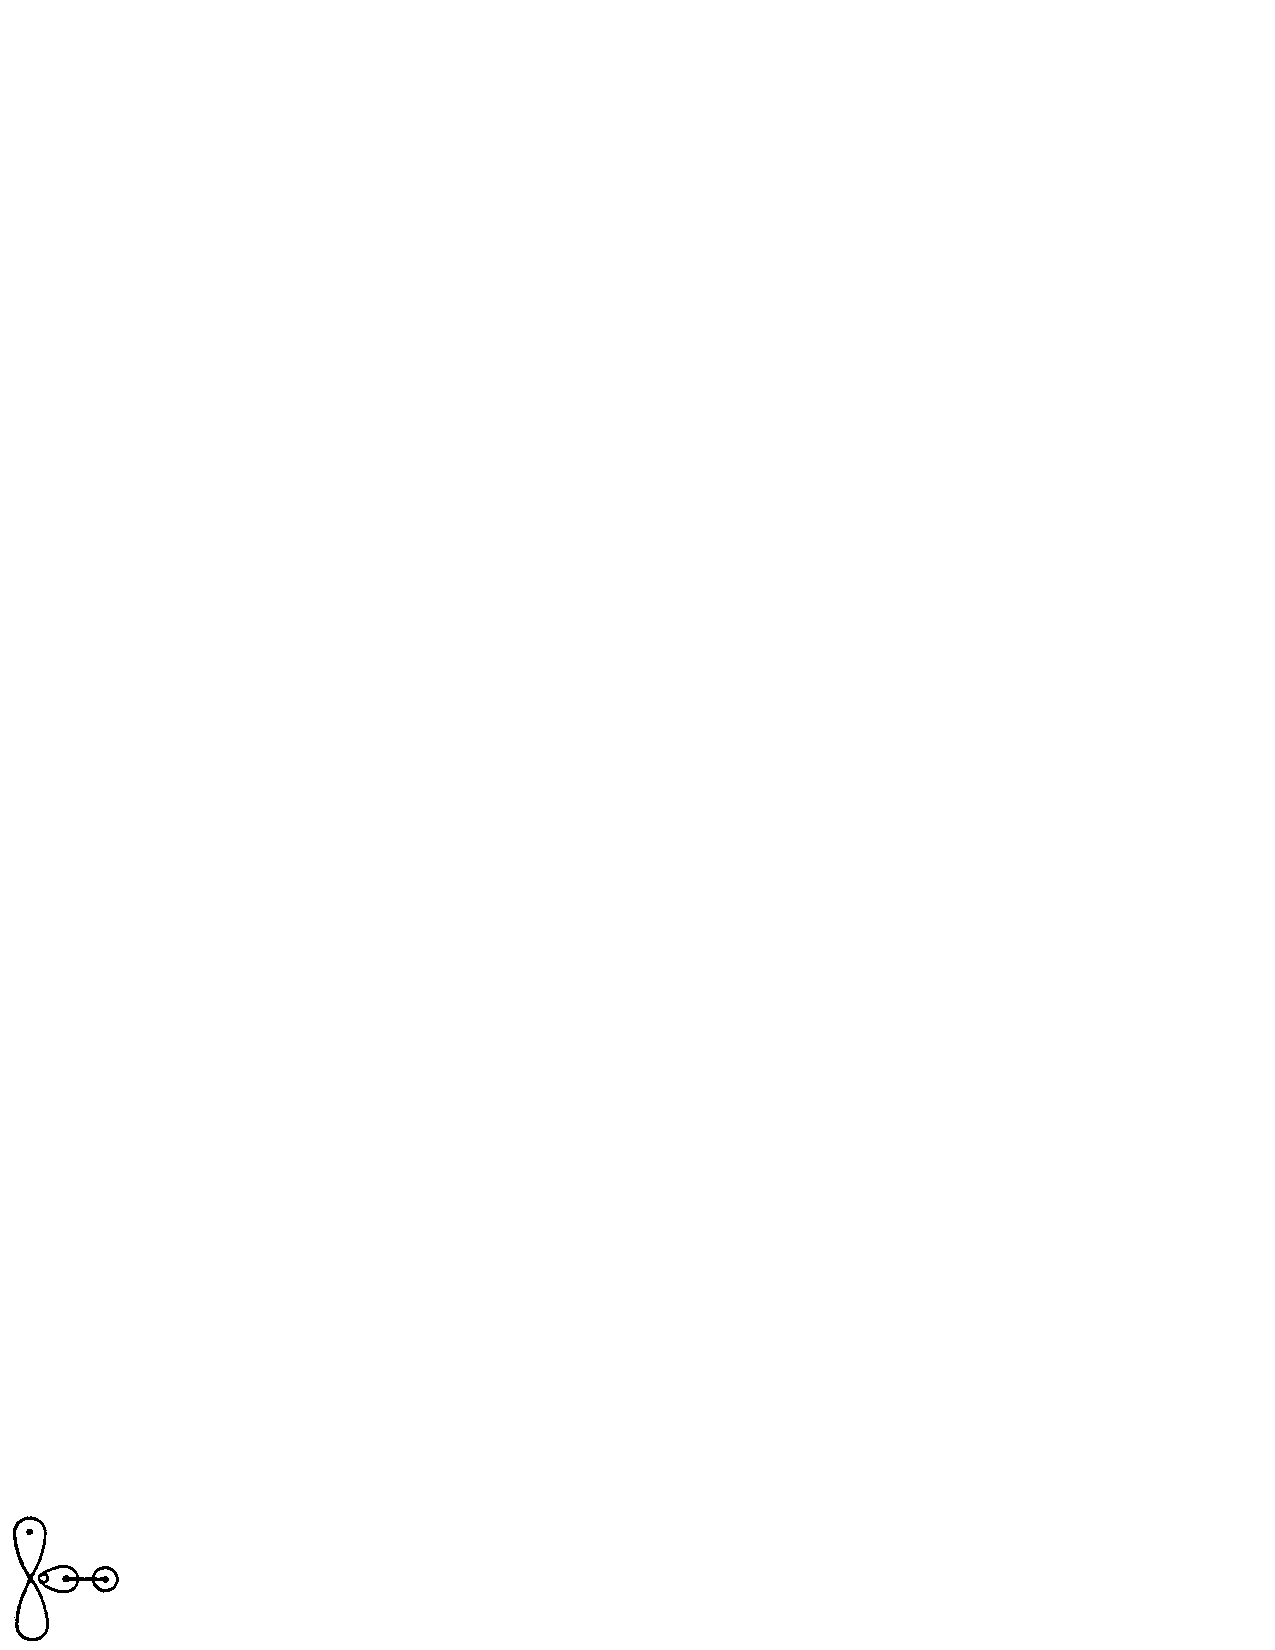
\includegraphics{fig6-10i}
\end{equation}
corresponding to exciting the nonbonding ${\bar{\ell}}$ orbital to a $3p$ 
orbital. This state dissociates to Mg(${^3P}$) rather than 
Mg$({^1S})$ and thus, the MgH ${^2\Sigma}^+
\rightarrow {^2\Pi}$ excitation energy, will be closely related to 
the atomic ${^1S} \rightarrow {^3P}$ excitation energy.  The potential 
curves for these states are shown schematically in Figure \ref{chap6-fig12}.

\begin{figure}
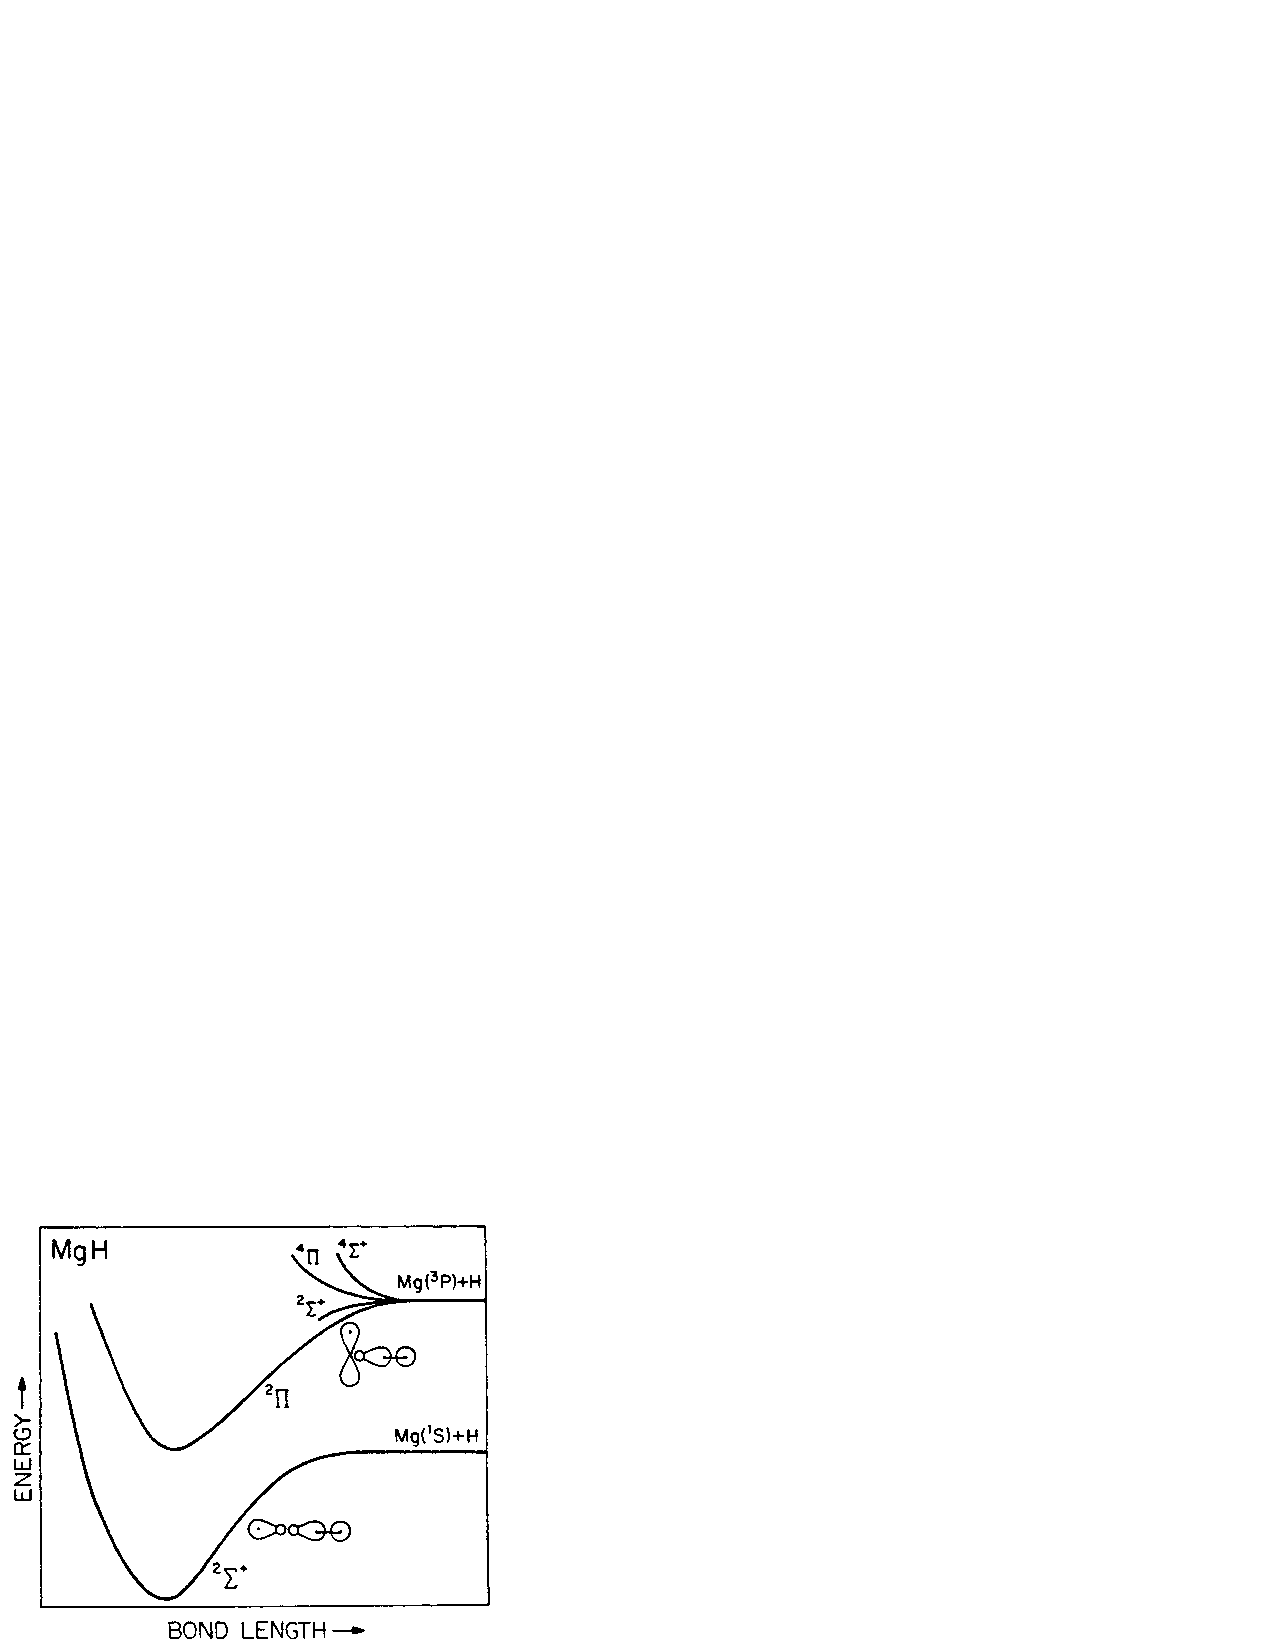
\includegraphics{fig6-11}
\caption{Schematic potential curves for MgH.}
\label{chap6-fig12}
\end{figure}

Exciting an orbital from the ground state of MgH$_2$,
(\ref{chap6-eqno21}) should lead to a state not bound, with respect to
H$ $+ MgH (${^2\Sigma}$).

\subsection{AlH$_n$}

In addition to the ${^1\Sigma}^+$ and ${^3\Pi}$ states of AlH,
(\ref{chap6-eqno45}) there are two other states dissociating to ground
state Al(${^2P}$). One is the ${^1\Pi}$ state, which has the orbital
occupation, shown earlier, but in which the two nonbonding orbitals,
${\bar{\ell}}$ and $\pi_x$ are singlet-paired.  The GVB
wavefunctions for the ${^3\Pi}$ state is
\begin{equation}
\psi ( {^3\Pi} ) = {\cal A} [ ( \phi_{\ell} \phi_\mathrm{H} + \phi_\mathrm{H} 
\phi_{\ell} ) ( \phi_{\bar{\ell}} \phi_{\pi_x} - \phi_{\pi_x} 
\phi_{\bar{\ell}} ) \alpha \beta \alpha \alpha ]
\end{equation}
and ${^1\Pi}$ state is
\begin{equation}
\psi ( {^1\Pi} ) = {\cal A} [ ( \phi_{\ell} \phi_\mathrm{H} + \phi_\mathrm{H} 
\phi_{\ell} ) ( \phi_{\bar{\ell}} \phi_{\pi_x} + \phi_{\pi_x} 
\phi_{\bar{\ell}} ) \alpha \beta \alpha \beta ]
\end{equation}
Using the same orbitals for these two states, this is, of course, an
approximation, leads to a ${^3\Pi} \rightarrow {^1\Pi}$ excitation
energy of $2K_{{\bar{\ell}},\pi_x}$ or about 40 kcal.  The second,
additional state, dissociating to Al(${^2P}$) is the ${^3\Sigma}^+$
state, which has the same orbital occupancy as the ${^1\Sigma}^+$
state, (\ref{chap6-eqno22}), but with the Al $p$ orbital triplet
coupled to the H orbital. The triplet coupling results in a repulsive
interaction and hence the ${^3\Sigma}^+$ state is not bound. The
potential curves for these four states of AlH, are shown in Figure
\ref{chap6-fig13}.

\begin{figure}
\includegraphics{fig6-12}
\caption{Schematic potential curves for AlH.}
\label{chap6-fig13}
\end{figure}

\begin{figure}
\includegraphics{fig6-13}
\caption{Schematic bending potential curves for AlH$_2$.}
\label{chap6-fig14}
\end{figure}

Consider next the ${^2{\cal A}}_1$  state of AH$_2$.  There is a low-lying,
unoccupied $p\pi$ orbital, perpendicular to the plane of the page.  
Thus, the
lowest excited state is expected to correspond to exciting the nonbonding
electron of the ${^2{\cal A}}_1$ state into the $p\pi$ orbital, as in
\begin{equation}
\includegraphics{fig6-13a}
\label{chap6-eqno35}
\end{equation}
Now consider how the orbitals of these two states, ${^2A}_1$ and 
${^2B}_1$, change as the bond angle is increased. The unpaired 
$\phi_{\bar{\ell}}$ orbital of the ${^2A}_1$ state, must remain 
orthogonal to the bond pairs, Pauli principle. Thus, as the bond angle is 
increased to 180$^{\circ}$, the $\phi_{\bar{\ell}}$ orbital deforms 
continuously into a $p$ orbital at 180$^{\circ}$,
\begin{equation}
\includegraphics{fig6-13b}
\label{chap6-eqno36}
\end{equation}
and the energy of the ${^2A}_1$ state increases as it is distorted 
to the linear geometry, since the optimum angle is 117$^{\circ}$.

As the ${^2B}_1$ state, (\ref{chap6-eqno35}), is distorted toward a
linear geometry, the nonbonding $p\pi$ orbital will not change
significantly, it is orthogonal to the bond pairs at all angles.
Thus, at a bond angle of 180$^{\circ}$ the ${^2B}_1$ state becomes
\begin{equation}
\includegraphics{fig6-13c}
\label{chap6-eqno37}
\end{equation}
with a $p\pi$ orbital out of the plane. For the ${^2B}_1$ state, since
both bonds are to lobe orbitals, the optimum geometry is the linear
one, (\ref{chap6-eqno37}), just as in MgH$_2$.  Thus, the energy of
the ${^2A}_1$ state increases as the molecule is made linear, while
the energy of the ${^2B}_1$ state decreases.

At the linear geometry, the two states (\ref{chap6-eqno36}) and
(\ref{chap6-eqno37}), are components for these two states as shown in
Figure \ref{chap6-fig14}.  Although AlH$_3$ has an empty $p\pi$
orbital, the excitation disrupts an A1H bond pair,
\begin{equation}
\includegraphics{fig6-13d}
\end{equation}
and, therefore will not be bound with respect to AlH$_2$ + H.

\subsection{SiH$_n$}

The lowest states of the SiH$_n$ molecules, were discussed
earlier.  Here we will discuss some of the important
higher lying excited states.

In addition to the ${^2\Pi}$ and ${^4\Sigma}^-$ states of SiH,
(\ref{chap6-eqno9} and (\ref{chap6-eqno10}), it is possible to
construct several doublet states using the orbitals of
(\ref{chap6-eqno10}). Ignoring the bond pairs, and taking the bond
axis to be $z$, these states have wavefunctions of the form
\begin{eqnarray}
{\rm SiH} ( {^4\Sigma}^- ) &:& {\cal A} \left[ \phi_{\bar{\ell}} 
\phi_{p_x} \phi_{p_y} \alpha \alpha \alpha \right]\cr
{\rm SiH} ( {^4\Delta}^- ) &:& {\cal A} \left[ \phi_{\bar{\ell}} 
\left( \phi_{p_x} \phi_{p_y} + \phi_{p_y} \phi_{p_x} \right) \alpha \alpha 
\beta \right]\cr
{\rm SiH} ( {^2\Delta}^+ ) &:& {\cal A} \left[ \phi_{\bar{\ell}} 
\left( \phi_{p_x} \phi_{p_x} - \phi_{p_y} \phi_{p_y} \right) \alpha \alpha 
\beta \right]\cr
{\rm SiH} ( {^2\Sigma}^+ ) &:& {\cal A} \left[ \phi_{\bar{\ell}} 
\left( \phi_{p_x} \phi_{p_x} + \phi_{p_y} \phi_{p_y} \right) \alpha \alpha 
\beta \right]\cr
{\rm SiH} ( {^2\Sigma}^+ ) &:& {\cal A} \left\{ \phi_{\bar{\ell}} 
\left( \phi_{p_x} \phi_{p_y} - \phi_{p_y} \phi_{p_x} \right) \left[ 
\beta \alpha \alpha - {1 \over 2} \alpha \left( \alpha \beta + \beta 
\alpha \right) \right] \right\}.
\end{eqnarray}
Note that the ${^4\Sigma}^-$, ${^2\Delta}^-$, and ${^2\Sigma}^-$ 
states, all have one electron in each of the
three nonbonding orbitals, and that these states differ only 
in the way the three orbitals are coupled.  There are three ways to 
couple the spins of three electrons,
one leads to a quartet, $S = 3/2$ state, while the other two lead to doublet,
$S = 1/2$ states.  Of the doublet states, one, the ${^2\Delta}^-$ state, 
has the two $p$
orbitals coupled into a singlet pair, low-spin.  While the other, 
$({^2\Sigma}^-)$ has
the two $p$ orbitals coupled into a triplet pair, high-spin. In both of the
doublet states, the ${\bar{\ell}}$ orbital is coupled to the $p_x - 
p_y$ pair to lead to an overall doublet state.

Although all five states involve similar orbitals, the two-electron
Coulomb and exchange terms differ. Since the three orbitals are
orthogonal, the state of highest multiplicity, ${^4\Sigma}^-$, is the
lowest in energy. The actual energy ordering of these states
is$^{10,21}$ ${^4\Sigma}^- < {^2\Delta} < {^2\Sigma}^- <
{^2\Sigma}^+$.  As the SiH molecule is dissociated, the ${^4\Sigma}^-$
and ${^2\Sigma}^-$ states, become components of Si(${^3P}$), while the
${^2 \Delta}$ and ${^2\Sigma}^+$ states, lead to Si(${^1D}$).  Thus, a
crossing of the ${^2 \Delta}$ and ${^2\Sigma}^-$ states, occurs at
some point along the potential curve.  One additional state,
dissociating to Si(${^3P}$) exists. This is the ${^4\Pi}$ state, which
has the same orbital occupation as the ${^2\Pi}$ state,
(\ref{chap6-eqno9}).  The difference being that the bond orbitals are
triplet-paired, leading to a repulsive potential curve. The potential
curves for the above states are shown schematically in Figure
\ref{chap6-fig15}.

\begin{figure}
\includegraphics{fig6-14}
\caption{Schematic potential curves for SiH.}
\label{chap6-fig15}
\end{figure}

\begin{figure}
\includegraphics{fig6-15}
\caption{Schematic bending potential curves for SiH$_2$.}
\label{chap6-fig16}
\end{figure}

Consider now the low-lying states of SiH$_2$. The first excited state
of SiH$_2$ is the ${^3B}_1$ state, (\ref{chap6-eqno14}).  This
configuration leads, however, to both a ${^3B}_1$ state and a
${^1B}_1$ state, depending upon whether the two nonbonding orbitals
are coupled high-spin or low-spin.  Using the same orbitals for both
states, the singlet-triplet separation is
\begin{equation}
\Delta E \left( {^1B}_1 \leftarrow {^3B}_1 \right) = 2 
K_{{\bar{\ell},p_x}}
\end{equation}
or about 30 kcal.$^{10,11}$  Solving self-consistently for the ${^3B}_1$ 
state, leads to a considerably larger
$K_{{\bar{\ell}},p_x}$, 28. 7 kcal, while solving for the ${^1B}_1$ 
state, leads to a smaller 
$K$, 13.2 kcal.  The value quoted here is for the average set of orbitals.

Increasing the bond angle of configuration (\ref{chap6-eqno14}) to
180$^{\circ}$ while keeping the ${\bar{\ell}}$ orbital orthogonal to
the bond pair (Pauli principle) leads to
\begin{equation}
\includegraphics{fig6-15a}
\end{equation}
Four states can be constructed, using the two $\pi$ orbitals of the 
above, ignoring the bond orbitals.
\begin{equation}
{\rm SiH}_2 \left( {^3\Sigma}^- \right) : {\cal A} \left[ \left( p_x 
p_y = p_y p_x \right) \alpha \alpha \right]
\label{chap6-eqno38}
\end{equation}
\begin{equation}
{\rm SiH}_2 \left( {^1\Delta}^- \right) : {\cal A} \left[ \left( p_x 
p_y + p_y p_x \right) \alpha \beta \right]
\label{chap6-eqno39}
\end{equation}
\begin{equation}
{\rm SiH}_2 \left( {^1\Delta}^+ \right) : {\cal A} \left[ \left( p_x 
p_x = p_y p_y \right) \alpha \beta \right]
\label{chap6-eqno40}
\end{equation}
\begin{equation}
{\rm SiH}_2 \left( {^1\Sigma}^+ \right) : {\cal A} \left[ \left( p_x 
p_x + p_y p_y \right) \alpha \beta \right]
\label{chap6-eqno41}
\end{equation}
Assuming the orbitals of all four states to be identical, and
equivalent, the one-electron part of the energy expression for states
(\ref{chap6-eqno38}) to (\ref{chap6-eqno41}) will be identical,
$2h_{pp}$.  The two-electron parts of the energy expressions, are
\begin{equation}
{^3\Sigma}^- : J_{xy} - K_{xy}
\label{chap6-eqno42}
\end{equation}
\begin{equation}
{^1\Delta}^- : J_{xy} + K_{yx}
\label{chap6-eqno43}
\end{equation}
\begin{equation}
{^1\Delta}^- : J_{xx} - K_{xy} = J_{xy} + K_{xy}
\label{chap6-eqno44}
\end{equation}
\begin{equation}
{^1\Sigma}^+ : J_{xx} + K_{xy} = J_{xy} + 3K_{xy}
\label{chap6-eqno45}
\end{equation}
where $J_{xx}$, $J_{xy}$, and $K_{xy}$ are the usual Coulomb and exchange 
integrals, and
we have made use of the equality of the${^1\Delta}^+$ and 
${^1\Delta}^-$  energies to rewrite the ${^1\Sigma}^+$ 
energy. Since $K_{xy} > 0$, the ${^3\Sigma}^-$ state is the ground 
state. As the bond
angle is increased from the equilibrium nonlinear geometries, to a linear
geometry, the three states discussed earlier correlate as
\begin{eqnarray}
&{^3B}_1 & \rightarrow {^3\Sigma}^-\cr
&{^1B}_1 & \rightarrow {^1\Delta}^-\cr
&{^1A}_1 & \rightarrow {^1\Delta}^+.
\label{chap6-eqno46}
\end{eqnarray}
The correspondence between the ${^1A}_1$ and ${^1\Delta}^+$ states,
(\ref{chap6-eqno46}), may not be clear.  Recall that the nonbonding
orbitals $\ell$ and ${\bar{\ell}}$ of the ${^1A}_1$ state,
(\ref{chap6-eqno12}), must remain orthogonal to the bond orbitals as
the bond angle is increased.  Consequently, at 180$^{\circ}$ these
orbitals are $p$ orbitals, bisecting the $x$ and $y$ axes, i.e., $\ell
\rightarrow p_x + p_y$, and ${\bar{\ell}} \rightarrow p_x - p_y$.
Therefore, the lone-pair part of the ${^1A}_1$ wavefunction becomes
\begin{equation}
\ell {\bar{\ell}} + {\bar{\ell}} \ell \rightarrow \left( p_x + p_y 
\right) \left( p_x - p_y \right) + \left( p_x - p_y \right) \left( 
p_x + p_y \right) = 2 \left( p_x p_x - p_y p_y \right),
\end{equation}
and, thus, the ${^1A}_1$ state correlates with the linear ${^1\Delta}^+$ state.

Consider now, the relative barriers to inversion of these states.
First, at their respective equilibrium, nonlinear geometries, the
${^1A}_1$ state is below the ${^3B}_1$, {\it vide supra}.  However,
from (\ref{chap6-eqno42}) to (\ref{chap6-eqno45}), the triplet is the
lowest state for the linear geometry.  Thus, the inversion barrier of
the ${^3B}_1$ state must be much lower than that of the ${^1A}_1$
state. Comparing, now, the ${^3B}_1$ and ${^1B}_1$ states, the only
difference in the energy expressions of these two states, is in the
sign of the exchange integral, $K_{{\bar{\ell}},p_x}$.  In fact,
assuming the orbitals of the two states to be identical, the ${^3B}_1
\rightarrow {^1B}_1$ excitation energy is just
$2K_{{\bar{\ell}},p_x}$.  At the linear geometry, this excitation
energy becomes $2K_{p_y,p_x}$.  Thus, since
\begin{equation}
K_{{\bar{\ell}},p_x} > K_{p_y,p_x},
\end{equation}
the linear energy separation is less than the nonlinear value.
Thus, the ${^1B}_1$ inversion barrier is slightly less than the 
${^3B}_1$. 	More qualitatively,
in making the ${^1A}_1$ state linear, two $p$ bonds must be converted 
to lobe bonds,
and hence, a large barrier is expected. For the ${^3B}_1$ and ${^1B}_1$
states, only one
$p$ bond must be converted to a lobe bond, and hence, a much smaller barrier
is expected.  The ${^1\Sigma}^+$, will have a linear equilibrium
geometry.  Qualitative potential curves for these four states are shown in
Figure \ref{chap6-fig16}.

\subsection{PH$_n$}

Before discussing the higher excited states of phosphorous hydrides,
we will first consider the low-lying excited states of atomic phosphorous 
having the same configuration, $(3s)^2 (3p)^3$, as the ground state. There 
are two such states, ${^2D}$ and ${^2P}$, consisting of a total of eight 
spatially distinct components.  Each of these component states 
involves either configurations such as shown earlier, with all three 
$p$ orbitals singly-occupied, or else the form
\begin{equation}
\includegraphics{fig6-15b}
\label{chap6-eqno47}
\end{equation}
in which one $p$ orbital is doubly-occupied, one is singly-occupied,
and one is unoccupied.  Since one of the $p$ orbitals of
(\ref{chap6-eqno47}) is empty, the GVB
description will involve a correlated $3s$ pair, as shown in
\begin{equation}
\includegraphics{fig6-15c}
\label{chap6-eqno48}
\end{equation}
This correlation is actually only important in the three components 
of the ${^2P}$ state, and does not play a role in the ${^2D}$ states.

Consider now the states of PH that can be constructed using the
orbitals of the ground state, (\ref{chap6-eqno25}).  Just as was found
with linear SiH$_2$, there are four such states, ${^3\Sigma}^-$,
${^1\Delta}^+$, ${^1\Delta}^-$, and ${^1\Sigma}^+$, with the
${^3\Sigma}^-$ state lowest, ground state, followed by the
${^1\Sigma}^+$ state.

The ${^1\Delta}^-$ state involves the same configuration as the
${^3\Sigma}^-$, (\ref{chap6-eqno25}).  However, the ${^1\Delta}^+$ and
${^1\Sigma}^+$ states are of the form
\begin{equation}
\includegraphics{fig6-15d}
\label{chap6-eqno49}
\end{equation}
Since there is an unoccupied $p$ orbital in both configurations, the 
GVB description leads to a correlated ($3s$) pair,
\begin{equation}
\includegraphics{fig6-15e}
\label{chap6-eqno50}
\end{equation}
This $3s$ correlation cancels in the ${^1\Delta}^+$ state, the minus
combination in (\ref{chap6-eqno49}).  Remember, the $3s$ pair is not
shown in (\ref{chap6-eqno49}) nor on the left side of
(\ref{chap6-eqno50}).  As found in the ${^2\Pi}$ state of SiH (Figure
\ref{chap6-fig2}) the lobe orbitals of (\ref{chap6-eqno50}) will be at
an angle of about 128$^{\circ}$ with respect to the bond.

Now consider bonding an H to an excited state of phosphorous,
(\ref{chap6-eqno48}).  Bonding to the singly-occupied $p$ orbital
leads to components of the ${^1\Sigma}^+$ and ${^1\Delta}^+$ states
discussed earlier.  Thus, upon dissociation, these states lead to
${^1D}$ phosphorous. Bonding to the lobe orbital of
(\ref{chap6-eqno48}) gives rise to the ${^3\Pi}$ and ${^1\Pi}$ states
of PH,
\begin{equation}
\includegraphics{fig6-15f}
\end{equation}
The lower of these two states, ${^3\Pi}$, is 84 kcal above the ground
state.  This large excitation energy results from two factors.  First,
the necessity of unpairing the lobe orbitals of (\ref{chap6-eqno48}),
and second, (\ref{chap6-eqno48}) itself corresponds to an excited
atomic state.  The potential curves for these states are shown in
Figure \ref{chap6-fig17}.

\begin{figure}
\begin{center}
\includegraphics{fig6-16}
\end{center}
\caption{Schematic potential curves for PH.}
\label{chap6-fig17}
\end{figure}

Bonding an H to a lobe orbital of (\ref{chap6-eqno50}) and allowing
for orbital readjustments, leads to the ${^2A}_1$ state of PH$_2$.
\begin{equation}
\includegraphics{fig6-17a}
\label{chap6-eqno51}
\end{equation}
As for SiH$_2$, the lobe-bond angle of PH is 128$^{\circ}$.  However,
repulsions between the incoming H orbital and the now unpaired lobe
orbital decrease the bond angle to about 118$^{\circ}$.  Increasing
the bond angle of (\ref{chap6-eqno51}) to 180$^{\circ}$ leads to one
component of the ${^2\Pi}$ state of linear PH$_2$,
\begin{equation}
\includegraphics{fig6-17b}
\end{equation}
The other component of the  ${^2\Pi}$ state,
\begin{equation}
\includegraphics{fig6-17c}
\end{equation}
correlates with the ${^2B}_1$ ground state,
(\ref{chap6-eqno26}). Recall that the $3s$ pair of
(\ref{chap6-eqno26}), not shown, must remain orthogonal to the bond
pairs as the bond angle is increased, and thus, correlates with a
$\pi$ pair of the linear molecule.  Schematic potential curves for
these two states are shown in Figure \ref{chap6-fig18}.

\begin{figure}
\includegraphics{fig6-17}
\begin{center}
\caption{Schematic bending potential curves for PH$_2$.}
\end{center}
\label{chap6-fig18}
\end{figure}

Starting with the ${^2A}_1$ state of PH$_2$, (\ref{chap6-eqno51}), and
bonding a third H, leads to the planar ${^1A}^{\prime}$ state of
PH$_3$,
\begin{equation}
\includegraphics{fig6-17d}
\end{equation}
The energy difference between this planar state and the pyramidal 
ground state of PH$_3$, is the barrier to inversion.  Recall that pyramidal
PH$_3$ involves three $p$ bonds to the ground state of phosphorous.  The 
planar state, however, involves one $p$ bond and two lobe bonds to an 
excited state of phosphorous.  Thus, the inversion barrier of PH$_3$ is 
expected to be much larger than that of SiH$_3$, where the barrier was 
just the difference between a lobe bond and a $p$ bond, approximately 21 
kcal. The actual barrier in PH$_3$ is approximately 37 kcal.$^{22}$

\subsection{SH$_n$}

Using the ground state configuration of atomic sulfur, $(3s)^2
(3p)^4$, we can construct two excited states, ${^1D}$ and ${^1S}$, in
addition to the ${^3}$P ground state. There are six spatially distinct
components of these states, three of the form shown earlier, and three
of the form
\begin{equation}
\includegraphics{fig6-17e}
\end{equation}
Since the above involves an unoccupied $p$ orbital, the GVB
description leads to a correlated ($3s$) pair,
\begin{equation}
\includegraphics{fig6-17f}
\label{chap6-eqno52}
\end{equation}
Bonding an H to one of the lobe orbitals of (\ref{chap6-eqno52}),
yields the ${^2\Sigma}^+$ state of SH,
\begin{equation}
\includegraphics{fig6-17g}
\label{chap6-eqno53}
\end{equation}
This state is very high-lying, approximately 84 kcal above the 
${^2\Pi}$, since it 
requires both an excited state of sulfur and the unpairing of the 
($3s$) lobe orbitals.  Schematic potential curves for these states are 
shown in Figure \ref{chap6-fig19}.

\begin{figure}
\includegraphics{fig6-18}
\caption{Schematic potential curves for SH.}
\label{chap6-fig19}
\end{figure}

Bonding an H to the unpaired lobe orbital of (\ref{chap6-eqno53}),
leads to the linear ${^1\Sigma}^+_g$ state of SH$_2$,
\begin{equation}
\includegraphics{fig6-18a}
\end{equation}
This configuration correlates with the ${^1A}_1$ ground state when the bond 
angle is decreased.  Thus, inversion of the ${^1A}_1$ state of SH$_2$ proceeds 
through a state in which both $p$ bonds of the ${^1A}_1$ state are replaced 
with lobe bonds, and in which an excited state of atomic sulfur is employed.


\section{Appendix}

In Chapter 2, we found that for a molecule with inversion symmetry, 
all eigenstates are either symmetric, $g$, or antisymmetric, $u$, 
under inversion, $i \psi_g = + \psi_g$ and $i \psi_u = - \psi_u$.  
Such symmetry information allows general considerations of the states 
of molecules, and often greatly simplifies the theoretical, or 
experimental, analysis of a 
system.  The most powerful theoems about symmetry are systematized 
under the title of group theory.  For most considerations, in 
chemistry and physics, the one aspect of group theory known as the 
theory of group representations, is most important.  For Chemistry 
120A, our only use of molecular symmetry will be in naming the 
symmetries.  Consequently, here we will summarize the names of the 
simple groups to be considered.  In Chemistry 120B, discussion of 
transition metal complexes will require more formal consideration of 
group theory.  The following pages are abstracted from a more complete 
discussion of group theory.

\subsection{Basis Concepts of Groups}

The symmetry group for a Hamiltonian ${\cal H}$ is the set of symmetry 
transformations ${\cal G}$, such that every element $R$ of ${\cal G}$ 
commutes with ${\cal H}$ in $R {\cal H} = {\cal H}R$.  Each such $R$, 
is referred to as a symmetry operation.

There are two types of symmetries which will be generally useful 
here.  First, permutation of the electrons or of equivalent nuclei, 
and second, spatial transformations, i.e., rotations, inversion, 
reflections, and translations, that result in merely permuting 
equivalent nuclei.  In order to be more precise about these 
symmetries, we must consider the specific forms of the wavefunctions 
and Hamiltonians to be solved.

\subsubsection{Electronic and Nuclear Wavefunctions}

The Hamiltonian for a molecule, has the form
\begin{equation}
{\cal H} = T^e + T^n + V^{en} + V^{ee} + V^{nn},
\label{chap6app-eqno1}
\end{equation}
where
\begin{eqnarray}
T^e &=& \sum^{Q}_{I=1} - {1 \over 2} \nabla^2_i\cr
T^n &=& \sum^{Q}_{I+1} - {1 \over 2M_I} \nabla^2_I\cr
V^{en} &=& \sum^{Q}_{I+1} \left( \sum^{N}_{i=1} - {Z_I \over r_{Ii}} 
\right)\cr
V^{ee} &=& \sum^{N}_{i>j=1} {1 \over r_{ij}}\cr
V^{nn} &=& \sum^{Q}_{I>J=1} {Z_IZ_J \over r_{IJ}}
\end{eqnarray}
and, $N$ and $Q$ are the number of electrons and nuclei, 
respectively.  The total wavefunction
\begin{equation}
\Psi \left( {\bf r}_1 \dots {\bf r}_N , {\bf R}_1 \dots {\bf R}_Q 
\right)
\end{equation}
is the eigenfunction of ${\cal H} \Psi = E \Psi$.

In the Born-Oppenheimer approximation, we take the total wavefunction 
to have the form
\begin{equation}
\Psi = \psi^{el} \Psi^{nuclear},
\end{equation}
where $\Psi^{nuclear}$ depends only on the $Q$ nuclear coordinates.  
The electronic wavefunctions,
\begin{equation}
\Psi^{el} \left( {\bf r}_1 , {\bf r}_2 , \dots , {\bf r}_N \right)
\end{equation}
are eigenstates of ${\cal H}^{el}$,
\begin{equation}
{\cal H}^{el} \Psi^{el} = E^{el} \Psi^{el},
\label{chap6app-eqno2}
\end{equation}
where
\begin{equation}
{\cal H}^{el} = T^e + V^{en} + V^{ee}
\end{equation}
is the electronic Hamiltonian, and where it is understood that in
(\ref{chap6app-eqno2}) the $Q$ nuclei are all fixed.  Thus,
$\Psi^{el}$ depends parametrically upon the $Q$ nuclear coordinates,
and $E^{el}$ is a function of these nuclear coordinates.  The
wavefunctions
\begin{equation}
\Psi^{nuclear} \left( {\bf R}_1 , {\bf R}_2 , \dots , {\bf R}_Q 
\right)
\end{equation}
are solutions of
\begin{equation}
{\cal H}^{nuclear} \Psi^{nuclear} = E \Psi^{nuclear}
\end{equation}
where
\begin{equation}
{\cal H}^{nuclear} = T^n + V^{nn} + E^{el}.
\end{equation}
In Chemistry 120, we will only be interested in the electronic 
wavefunctions of (\ref{chap6app-eqno2}).

\subsubsection{Types of Symemtries}

The terms $T^e$, $V^{en}$, and $V^{ee}$ of (\ref{chap6app-eqno1}) are
invariant under any of the $N!$ possible permutations, renumberings,
of the $N$ electrons.  Consequently, these $N!$ permutations of
electrons are contained in the symmetry groups of ${\cal H}^{el}$ and
of ${\cal H}$.

Similarly, ${\cal H}^{el}$ and ${\cal H}$ are invariant under any 
permutation of equivalent nuclei among each other.  Actually, ${\cal 
H}^{el}$ has a higher symmetry here, since it is invariant under any 
permutation of nuclei having the same charge, whereas with ${\cal H}$ 
the permutated nuclei must have the same charge and mass.

Both ${\cal H}$ and ${\cal H}^{el}$ are invariant under any spatial 
transformation that preserves the lengths of all inter-particle 
coordianes.  The general transformations satisfying this condition 
are, first, rotations about some axis, second, inversion through some 
point, third, reflection throug some plane, and fourth, translation 
along some axis, and the various combinations of the above 
operations.  Next, we develop some important concepts of symmetry 
groups.

\subsubsection{Basic Spatial Symmetry Operations}

Consider a square.  A counter clockwise rotaton of 90$^{\circ}$, which
will be denoted (for \emph{cyclisch}, German for cyclic) as $C_4$,
leaves the square in a configuration indistinguishable from the
original,

$C_4$

\noindent
and hence, we call $C_4$ a symmetry operation, of the square.  We 
number the corners of the square to keep track of what we are doing.  
If the numbers were actually printed on the square, there would be no 
symmetry.  Applying $C_4$ again

$C^2_4$

\noindent
gives an equivalent configuration and, hence, $C^2_4$ is also a 
symmery operation.  Continuing in this way, we find that $C^n_4 = C_4 
C_4 \dots C_4$, is a symmetry operation for any $n$.  Of course, 
$C^4_4$ corresponds to a rotation through 360$^{\circ}$, which is 
equivalent to no rotation whatsoever.  The operation of doing nothing, 
that is, the identity operation, is denoted by $e$ (for \emph{einheit}
meaning unity in German).  Thus, we have
\begin{equation}
C^4_4 = e
\end{equation}
and
\begin{equation}
C^{n-4}_4 = C^n_4 .
\end{equation}

There are other symmetry operations for a square, such as 
reflections, in a plane, denoted by $\sigma$ for spiegel in German, 
e.g.,

$\sigma$

\noindent
and inversion through a point, denoted by $i$, e.g.,

$i$

\noindent
In general, we will use the following notations for symmetry 
operations.  $C_n$ for counter-couckwise rotation of $(2\pi/n)$ 
radians about some axis of symmetry. $\sigma$ for reflection in some 
plane of symmetry.  $i$ for inversion through some point or center of 
symmetry.  $S_n$ for rotary reflection, notation $C_n$ followed by a 
reflection, $\sigma_h$, in a plane perpendicular to the rotation axis
\begin{equation}
S_n = \sigma_h C_n
\end{equation}
All of the above operations, are referred to as point operations such 
they leave invariant at least one point in space.  There are a number 
of other symmetry transformations involving translation of the system 
along some axis followed, perhaps, by one or more of the above point 
operations.  Although such symmetries are of particular importance in 
discussing solids, we will ignore them here.

\subsubsection{The Properties of a Group}

It is clear, given two symmetry operations, ${\hat{R}}_1$ and 
${\hat{R}}_2$ for some object, the product ${\hat{R}}_1 
{\hat{R}}_2$, denoting the application of the first ${\hat{R}}_2$ and 
then ${\hat{R}}_1$, is also a symmetry operation.  For example, 
rotating ethylene 180$^{\circ}$ about the CC axis, and then reflecting 
in the perpendicular plane bisecting the CC bond, also leaves the 
molecule invariant

\noindent
Consequently, the set of all symmetry operations for any object is 
closed under multiplication.  That is, letting ${\cal G}$ denote the 
set of all symmetry operations, if $R_1$ is a member of ${\cal G}$, 
denoted as $R_1 \epsilon {\cal G}$, and $R_2 \epsilon {\cal G}$, the 
$R_1R_2 \epsilon {\cal G}$ and $R_2R_1 \epsilon {\cal G}$.  
$R_1\epsilon {\cal G}$ is read as $R_1$ is an element of ${\cal G}$.

It is also clear that the multiplication is associative, i.e. for 
$R_1$, $R_2$, $R_3 \epsilon {\cal G}$, then
\begin{equation}
\left( R_1 R_2 \right) R_3 = R_1 \left( R_2 R_3 \right) .
\end{equation}
In our discussion, the $R_i$ are considered operations.  Thus, an 
equation such as above, is interpreted as saying the $(R_1R_2)R_3$ 
operating on an object, leads to a result equivalent to that obtained 
by $R_1(R_2R_3)$ operating on our object.

The identity operator, $e$, is always a member of ${\cal G}$.  Since 
$e$ does nothing, we see that $Re = eR = R$; that is, $e$ commutes 
with all elements of the group.

If $S$ and $R$ have the property that
$S R = e$, we refer to $S$ as the inverse of $R$, and denote it as
$S = R^{-1}$.  It is easy to see that if $R$ is a symmetry operation, 
then $R^{-1}$ is also a symmetry operation.  That is, $R \epsilon 
{\cal G}$ implies 
that there is also another element, $R^{-1} \epsilon {\cal G}$, such that
$R R^{-1} = R^{-1} R = e$.  
These properties of ${\cal G}$, the set of symmetry operations, 
correspond to the properties of a group, generally defined as follows.

\subsubsection{Definition of a Group}

The group, ${\cal G}$ is a set of elements $\{R_i\}$ with a specified 
law of multiplication, satisfying the following properties.  First,
There exists an element $e \epsilon {\cal G}$, called the identity such that
$eR =Re =R$ for all $R \epsilon {\cal G}$.  Second, 
for every element $R \epsilon {\cal G}$, there exists an element 
$R^{-1} \epsilon {\cal G}$, called the inverse of $R$, such that
$RR^{-1} = R^{-1} R = e$.  Third, the group is closed under 
multiplication, closure, i.e., 
if $R_1 \epsilon {\cal G}$ and $R_2 \epsilon {\cal G}$, then $R_1R_2 
\epsilon {\cal G}$.  Fourth, the group multiplication is associative,
$(R_1R_2)R_3 = R_1 (R_2R_3)$.  The number of elements, $g$, in the 
group, ${\cal G} = \{ e , R_2 , \dots , R_g \}$ is 
called the order of the group.

The above properties lead to severe restrictions upon the permitted 
multiplication laws, and indeed for groups of finite order there are 
only a finite number of possible groups.  Note, in particular, that the 
definition of a group does not impart to the $R_i$ any significance 
beyond the multiplication law.  Thus, the $R_i$ need not correspond to 
operations upon some sort of object.
	
Group theory is the study of the properties of groups. This theory
has led to a number of powerful theorems that allow classification of groups
into different types and provide an analysis of the forms for various types
of groups.  We will be interested only in groups whose elements lead to
transformations upon some set of objects. This simplifies the group theory.
In addition, we will be interested mainly in the
special part of group theory known as the theory of group representations.
A group can be of finite order, as in the case of a square, or of infinite
order, as in the case of a sphere. An example of an important infinite
group is the group of all rotations, about some point, in three dimensions,
denoted as SO(3).

Note that the law of multiplication need not be communicative, that is
$R_1 R_2 \not= R_2 R_1$ in general.  For example,

$C_4 \sigma$

$\sigma C_4$

\noindent
and, hence, $C_2 \sigma \not= \sigma C_4$.  If $R_1R_2 = R_2 R_1$, 
we say that $R_1$ and $R_2$ commute.  If all elements of a 
group commute with each other, the group is referred to as an Abelian group.

Given some set of elements
\begin{equation}
{\cal S} = \left\{ R_1 , R_2 , \dots , R_s \right\}
\end{equation}
and a law for multiplying them, we can form a group ${\cal G}$ by 
taking all possible products,
any number of terms, of the elements of	${\cal S}$, and 
collecting all the elements
so obtained into ${\cal G}$.  A set of elements	${\cal S}$, 
leading in this way to a group ${\cal G}$
are referred to as the generators of ${\cal G}$.  For example, starting
with of	${\cal S} = \{ C_4 \}$,	we obtain the group
\begin{equation}
{\cal G} = \left\{ e , C_4 , C^2_4 , C^3_4 \right\}.
\end{equation}
Similarly, starting with
\begin{equation}
{\cal S} = \left\{ C_2 , C_3 \right\}
\end{equation}
where
\begin{equation}
C^{-1}_3 = C_2 C_3 C_2 ,
\end{equation}
i. e., $C_2$ and $C_3$ are at right angles, leads to the group
\begin{equation}
{\cal G} = \left\{ e , C_3 , C^{-1}_3 , C_2 , C_2 C_3 , C_3 C_2 
\right\}.
\end{equation}

\subsubsection{Classes}

We will find it convenient to partition each group into, mutally
exclusive, sets of elements, called classes, such that two elements, 
$S$ and $T$, of a class are related to each other by$S = RTR^{-1}$,
where $R$ is the same element $R$ of the same group ${\cal G}$. 
Transformations of the same class are always of equivalent form, e.g., all are 
reflections or all are rotations through an angle of 120$^{\circ}$.

\subsection{Some Important Molecular Symmetry Groups}

\subsubsection{$C_{2v}$}

Consider an AH$_2$ molecule with equal bond lengths,

\noindent
The symmetry operators are
\begin{description}
\item[$e$] \emph{einheit} (unity)
$x \rightarrow x$, $y \rightarrow y$, and $z \rightarrow z$.  
\item[$C_{2z}$] a rotation of 180$^{\circ}$ about the $z$ axis, $z 
\rightarrow z$, $x \rightarrow -x$, and $y \rightarrow -y$. 
\item[$\sigma_{xz}$] a reflection through the $xz$ plane, $z \rightarrow 
z$, $x \rightarrow x$, and $y \rightarrow -y$.  
\item[$\sigma_{yz}$] 
a reflection through the molecular plane, $z \rightarrow z$, $x 
\rightarrow -x$ and $y \rightarrow y$.
\end{description}
The group $\{ e , C_{2z}, 
\sigma_{xz}, \sigma_{yz} \}$ is denoted {\bf C}$_{2z}$.  The basic 
symmetries, usually called \emph{irreducible representations}, are
\begin{center}
\begin{tabular}{c|cccc|l}\\
& $e$ & {\bf C}$_{2z}$ & $\sigma_{xz}$ & $\sigma^{\prime}_{yz}$ &\cr
\hline
$A_1 $ & 1 & 1 & 1 & 1 & $s , p_z, d_{z^2} , d_{x^2-y^2}$\cr
$A_2$ & 1 & 1 & $-1$ & $-1$ & $d_{xy}$\cr
$B_1$ & 1 & $-1$ & 1 & $-1$ & $p_x , d_{xz}$\cr
$B_2$ & 1 & $-1$ & $-1$ & 1 & $p_y , d_{yz}$\cr
\end{tabular}
\end{center}
where at the right, we show the symmetries for atomic orbitals, centered 
on $A$.  Such a table is usually called a character table.

Items to note here are, first, that $B_1$ and $A_2$ 
are antisymmetric with respect to reflection in the
molecular plane, often referred to as $\sigma$ states.  Second, $B_2$ 
and $A_2$ are antisymmetric with respect to the reflection in
interchanging the $H$'s, often referred to as $\pi$ states.

For planar molecules, it is customary to refer to orbitals that are
symmetric with regard to the molecular plane as $\sigma$ functions, and to refer
to orbitals that are antisymmetric, with regard to the molecular plane as
$\pi$ functions.  It should be noted that the $\sigma$ and $\pi$ 
so used, need not be related to the $\sigma$ and $\pi$ we use in 
discussing linear molecules. In the latter case, $\sigma$ and $\pi$ 
refer to rotation symmetry, whereas for the planar
molecule, $\sigma$ and $\pi$ refer to reflection symmetry.

For example, for a diatomic molecule oriented along the $z$ axis, we 
have equivalent $\pi_x$ and $\pi_y$ orbitals

\noindent
Classifying these states, with respect to the $C_{2v}$ group, leads to
$D_{\infty h} C_{2v}$, $\pi_y \rightarrow \sigma (B_2)$, and $\pi_x 
\rightarrow \pi (B_1)$.

For a many-electron wavefunction, we must consider the simultaneous 
transformation of all orbitals in order to determine the symmetry.  As 
an example, consider the ${^1A}_1$ wavefunction for SiH$_2$,

\begin{equation}
\Psi_1 = {\cal A} \left[ \Phi_{core} \left( pH = Hp \right) \alpha 
\beta \left( {\bar{p}} {\bar{H}} + {\bar{H}} {\bar{p}} \right) 
\alpha \beta \left( s x s {\bar{x}} + s {\bar{x}} sx \right) \alpha 
\beta \right] .
\end{equation}
Applying $C_{2z}$ leads to $p \leftrightarrow {\bar{p}}, H 
\leftrightarrow {\bar{H}}, sx \leftrightarrow s {\bar{x}}$, and, 
$\Phi_{core} \rightarrow \Phi_{core}$, and hence,
\begin{equation}
C_{2z} \Psi_1 = {\cal A} \left[ \Phi_{core} 
\underbrace{({\bar{p}}{\bar{H}}+{\bar{H}}{\bar{p}})\alpha \beta 
(pH+HP)\alpha \beta}_{(pH+Hp)\alpha 
\beta({\bar{p}}{\bar{H}}+{\bar{H}}{\bar{p}}+{\bar{H}}{\bar{p}})\alpha 
\beta} 
\underbrace{(s{\bar{x}}sx+sxs{\bar{x}})}_{(sxs{\bar{x}}+s{\bar{x}}sx)} 
\alpha \beta \right]
\end{equation}
but
\begin{equation}
\left( s {\bar{x}} sx + sxs{\bar{x}} \right) = \left( sxs{\bar{x}} + 
s {\bar{x}} sx\right)
\end{equation}
and
\begin{equation}
{\cal A} \left( {\bar{p}} {\bar{H}} + {\bar{H}} {\bar{p}} \right) 
\alpha \beta \left( pH + Hp \right) \alpha \beta = {\cal A} \left( 
pH + Hp \right) \alpha \beta \left( {\bar{p}} {\bar{H}} + {\bar{H}} 
{\bar{p}} \right) \alpha \beta
\end{equation}
interchanging two pairs of electrons.  Hence,
\begin{equation}
C_{2z} \Psi_1 = \Psi_1 .
\end{equation}
Similarly,
\begin{equation}
\sigma_{xz} \Psi_1 = \Psi_1
\end{equation}
and
\begin{equation}
\sigma_{yz} \Psi_1 - \Psi_1
\end{equation}
and, hence, $\Psi_1$ is ${^1A}_1$.

For the ${^3B}_1$ state of SiH$_2$

\noindent
the wavefunction is
\begin{equation}
\Psi_2 = {\cal A} \left[ \Phi_{core} ( pH + Hp ) \alpha \beta ( 
{\bar{p}} {\bar{H}} + {\bar{H}} {\bar{p}} ) \alpha \beta ( \sigma 
\pi - \pi \sigma ) \alpha \alpha \right] .
\end{equation}
Under the symmetry operations, the bond pairs behave as in the 
${^1A}_1$  
state, and the $\sigma$ orbital is unaffected by all operators, and
$C_{2z} \pi = - \pi$ thus, $C_{2z} \Psi_2 = - \Psi_2$; $\sigma_+{xz} 
\pi = \pi$ thus, $\sigma_{xz} \Psi_2 = \Psi_2$; and, $\sigma_{yz} 
\pi = - \pi$ thus, $\sigma_{yz} \Psi_2 = - \Psi_2$.  Thus, $\Psi_2$ 
is ${^3B}_1$.

\subsubsection{$C_v$}

Consider the nonplanar AH$_3$ molecule,
\begin{equation}
% need a picture of AH3 from p6-a-14
\end{equation}
where $z$ is the three-fold symmetry axis. The symmetry operations are
\begin{description}
\item[$e$] einheit or unity;
\item[$C_{3z}$]
a counter clockwise rotation of 120$^{\circ}$ about the $z$ axis,
\item[$C^{-1}_{3z}$] a clockwise rotation of 120$^{\circ}$ about the $z$ 
axis.  
\item[$\sigma_{xz}$] a reflection in the $xz$ plane,  
\item[$\sigma^{\prime}$] for 
a reflection in the plane containing the AH$_2$ axis and the $z$ 
axis.  
\item[$\sigma^{\prime \prime}$] for 
a reflection in the plane containing the AH$_3$ axis and the $z$ axis, 
\end{description}
and the group is denoted {\bf C}$_{3v}$.  The basic symmetries are
\begin{center}
\begin{tabular}{c|ccc|l}
& $e$ & $\{ C_3,C^{-1}_3\}$ & $\{ \sigma_{xz} , \sigma^{\prime} , 
\sigma^{\prime \prime}\}$\cr
\hline
$A_1$ & 1 & 1 & 1 & $s, p_z , d_{z^2}$\cr
$A_2$ & 1 & 1 & $-1$ &\cr
$E$ & 2 & $-1$ & 0 & $\{p_x,p_y\},\{d_{xy},d_{x^2-y^2}\},\{d_{xz}, 
d_{yz}\}$\cr
\end{tabular}
\end{center}

Here, $E$ contains two functions, $E_x$ and $E_y$, that are intermixed by the 
symmetry operations.  For example, consider $p_x$ and $p_y$ functions 
centered on $A$,
\begin{eqnarray}
C_3p_x &=& - {1 \over 2} p_x + {\sqrt{3} \over 2} p_y\cr
C_3 p_y &=& - {\sqrt{3} \over 2} p_x - {1 \over 2} p_y\cr 
\Rightarrow D(C_3) = {\pmatrix{-{1 \over 2} & - {\sqrt{3} \over 2}\cr
{\sqrt{3} \over 2} & - {1 \over 2}}}
\end{eqnarray}
\begin{eqnarray}
\sigma_{xz}p_x &=& p+x\cr
\sigma_{xz} p_y &=& -p_y\cr
\Rightarrow D \left( 
\sigma_{xz} \right) = {\pmatrix{1 & 0\cr 0 & -1}}
\end{eqnarray}
and
\begin{eqnarray}
\sigma^{\prime} p_x &=& - {1 \over 2} p_x - {\sqrt{3} \over 2} p_y\cr
\sigma^{\prime} p_y &=& - {\sqrt{3} \over 2} p_x + {1 \over 2} 
p_y\cr
\Rightarrow D \left( \sigma^{\prime} \right) = 
{\pmatrix{-{1 \over 2} & - {\sqrt{3} \over 2}\cr
-{\sqrt{3} \over 2} & {1 \over 2}\cr}}
\end{eqnarray}
This is calculated most easily, using the relation
\begin{equation}
\sigma^{\prime} = C_3 \sigma_{xz} C^{-01}_3
\end{equation}
and, hence
\begin{equation}
D(\sigma^{\prime} ) = D(C_3 )D(\sigma_{xz} ) D ( C^{-1}_3 ).
\end{equation}
In general, we write
\begin{equation}
R \phi_i = \sum_{j} \phi_j D_{ji} (R) ,
\end{equation}
and in the symmetry table, we list the trace, called the character, 
of the matrix $D(R)$. Note that similar operators have the same character.

\subsubsection{C$_{\infty v}$}

For a linear molecule, axis along $z$, the symmetry operators are
\begin{description}
\item[$e$] einheit.  
\item[$R_x(\alpha)$]
counter clockwise rotation by an angle $\alpha$ about the $z$ axis.  
\item[$\sigma_{xz}$] for reflection in the $xz$ plane.  
\item[$\sigma^{\prime} = 
R_z(\alpha)\sigma_{xz} R_z(-\alpha)$] for
reflection in a plane rotated by an angle $\alpha$ from the $xz$
plane, there are an infinite number of these,
\end{description}
and the group is 
denoted as {\bf C}$_{\infty v}$. 
The symmetry functions for {\bf 
C}$_{\infty v}$ are
\begin{description}
\item[$\Sigma^+$] unchanged by all operations  
\item[$\Sigma^-$] unchanged by all rotations, changes sign under all 
reflections,  
\item[$\Pi$] two functions, $\pi_x$ and $\pi_y$, that change like
$\cos \phi$ and $\sin \phi$ under the operations of {\bf C}$_{\infty 
v}$. $\phi$ is the angle about the $z$ axis with $\phi = 0$ lying in 
the $xz$ plane,  
\item[$\Delta$] two functions, $\Delta_{xy}$ and 
$\Delta_{x^2-y^2}$, that change like $\cos 2 \phi$ and $\sin 2 \phi$ 
under {\bf C}$_{\infty v}$,  
\item[$\Phi$] two functions that change like 
cos $3\phi$ and sin $3\phi$ under {\bf C}$_{\infty v}$,
\item[$\Gamma$] two functions that change like cos $4 \phi$ and sin $4
\phi$ under {\bf C}$_{\infty v}$
\end{description}
Lower case letters are used to denote one-electron orbitals 
having the above symmetries, e.g., $\sigma$ for $\Sigma^+$, $\pi$ 
for $\Pi$, $\delta$ for $\Delta$, $\phi$ for $\Phi$, $\gamma$ 
for $\Gamma$, etc.

The symmetry table is
\begin{center}
\begin{tabular}{c|ccc|l}
& $e$ & $R(\alpha)$ & $\{\sigma_{xz}\sigma^{\prime}\}$\cr
\hline
$\Sigma^+$ & 1 & 1 & 1 & $s , p_z , d_{z^2}$\cr
$\Sigma^-$ & 1 & 1 & $-1$\cr
$\Pi$ & 1 & 2 cos $\alpha$ & 0 & $\{p_x , p_y\},\{d_{xz} , d_{yz} 
\}$\cr
$\Delta$ & 1 & 2 cos 2$\alpha$ & 0 & $\{d_{xy},d_{x^2-y^2}\}$\cr
$\Phi$ & 2 & 2 cos 3$\alpha$ & 0\cr
$\Lambda$ & 2 & 2 cos 4$\alpha$ & 0\cr
\end{tabular}
\end{center}
